% Created 2022-09-30 ven 12:10
% Intended LaTeX compiler: pdflatex
\documentclass[10pt]{report}
\usepackage[utf8]{inputenc}
\usepackage[T1]{fontenc}
\usepackage{graphicx}
\usepackage{longtable}
\usepackage{wrapfig}
\usepackage{rotating}
\usepackage[normalem]{ulem}
\usepackage{amsmath}
\usepackage{amssymb}
\usepackage{capt-of}
\usepackage{hyperref}
\usepackage[a4paper, inner=4.1cm, outer=4.1cm, tmargin=2.7cm, bmargin=3.0cm]{geometry} % Sets margins and borders
\usepackage[document]{ragged2e}
\setlength{\parindent}{0cm}
\usepackage[T1]{fontenc}
\usepackage[utf8]{inputenc}
\usepackage{amsmath}
\usepackage{amssymb}
\usepackage{gensymb}
\usepackage{cancel}
\usepackage{mathtools}
\usepackage{mlmodern}
\usepackage{hyperref}
\usepackage{graphicx}
\usepackage{makecell}
\usepackage[all]{nowidow}
\usepackage{parskip}
\usepackage{setspace}
\setstretch{1.35}
\setcounter{MaxMatrixCols}{20}
\usepackage{fancyhdr}
\pagestyle{fancy}
\fancyhf{}
\fancyhead[LE,RO]{\leftmark}
\fancyfoot[LE,RO]{\thepage}
\renewcommand{\headrulewidth}{1pt}
\newtheorem{theorem}{Theorem}[theorem]
\author{Marco Sgobino}
\date{\today}
\title{Computer Vision Study Guide}
\hypersetup{
 pdfauthor={Marco Sgobino},
 pdftitle={Computer Vision Study Guide},
 pdfkeywords={},
 pdfsubject={},
 pdfcreator={Emacs 28.1 (Org mode 9.6)}, 
 pdflang={English}}
\begin{document}

\begin{titlepage}
\begin{center}
\Large
\textbf{UNIVERSITÀ DEGLI STUDI DI TRIESTE}
\par\noindent\rule{\textwidth}{1.8pt}
\vspace*{0.6cm}
\large

\emph{Marco Sgobino}

\large
\vspace*{0.6cm}
\Large Notes from the course of

\vspace*{0.6cm}
\Huge
\textsc{Computer Vision and Pattern Recognition}

\vspace*{.1cm}
\vspace*{2cm}
\begin{center}
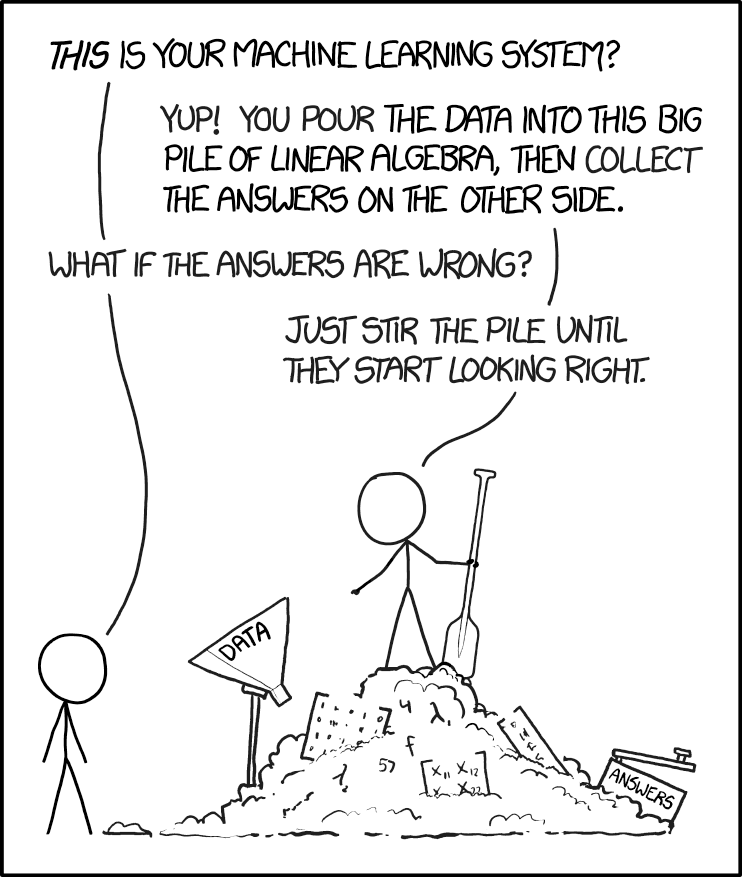
\includegraphics[width=.6\textwidth, keepaspectratio]{./pics/cv-titlepage.png}
\end{center}
\vfill
\par\noindent\rule{\textwidth}{1.8pt}
\vspace*{0.6cm}
\large
\emph{Academic Year 2021-2022}
\end{center}
\end{titlepage}
\tableofcontents


\part{Introduction}
\label{sec:org5a265cc}
\setstretch{1.25}
\setlength{\headsep}{30pt}
\setlength{\footskip}{40pt}
\setlength{\marginparsep}{20pt}
\setlength{\marginparwidth}{60pt}
\chapter{The Computer Vision}
\label{the-computer-vision}
\section{The definition of Computer Vision}
\label{the-definition-of-computer-vision}
What is \emph{Computer Vision}?

Computer Vision is the science of \textbf{getting the machines see}. Another
definition could be such that

\begin{quote}
\emph{Computer vision is concerned with the automatic extraction, analysis and understanding of useful information from a single image or a sequence of images. It involves the development of a theoretical and algorithmic basis to achieve automatic visual understanding.}
\end{quote}

Other definitions are the following ones,

\begin{itemize}
\item computing properties of the 3-D world from one or more digital images;
\item to make useful decisions about real physical objects and scenes based
on sensed images; the construction of explicit, meaningful description
of physical objects from images; extracting descriptions of the world
from pictures or sequences of pictures.
\end{itemize}

Computer vision is strictly related to various sciences, for instance,
\emph{optics}, \emph{machine learning}, \emph{neuroscience}, \emph{mathematics}, \emph{cognitive
sciences}, \emph{image processing} and \emph{computer science} in general.

Computers usually see through bidimensional images; all the necessary
three--dimensional information should be extracted directly from the
image. In particular, one is interested into:

\begin{itemize}
\item \emph{semantic information}, the ``what'';
\item \emph{three--dimensional metric information}, the ``where''.
\end{itemize}

By combining the previous two kind of informations, one is able to
deeply understand an image, its content, and ultimately its meaning. One
of the goals of computer vision is to bridge the gap between the pixel
representation of an image and its \emph{meaning}, so that a machine can
perform specific tasks.

Object in images are subjected to many kinds of variations:

\begin{itemize}
\item objects are subjected to different \textbf{illuminations}; they can be dark,
bright, over--exposed or under--exposed;
\item to different \textbf{occlusion}; they can be partially hidden, not having all
their shape exposed to the viewer;
\item to \textbf{deformation}; their shape can
be deformed for perspective reasons or because of their own movement;
\item they could blend with the \textbf{background}; object textures could be very
similar to those of the background, resulting in difficult detection;
\item there could be many instances, with different classes (\textbf{intraclass
variation}).
\end{itemize}

All these variations pose serious challenges to identifying what is
present in an image.

Regarding the ``where'', the problem of locating objects in
two--dimensional images is said to be \textbf{ill-posed} in contrast to
\textbf{well-posed} problems. An example of a well-posed problem is the forward
problem of building an image from three--dimensional information.

The ill-posed nature of the problem lies to resides in the fact that
many explanations exist for a single image.

\section{Classes of problems in CV}
\label{classes-of-problems-in-cv}
\begin{quote}
\emph{The first great revelation was that the problems are difficult. Of course, these days this fact is a com- monplace. But in the 1960s almost no one realized that machine vision was difficult. The field had to go through the same experience as the machine translation field did in its fiascoes of the 1950s before it was at least realized that here were some problems that had to be taken seriously.}
\end{quote}

Two classes of computer vision problem exist. The first class is the \textbf{recognition} class. Recognition task involves different tasks,

\begin{itemize}
\item \emph{object detection}, find all the regions in an image belonging to a certain object, or that are likely to belong to a certain object);
\item \emph{instance recognition}, determine an instance of an already known object, potentially being viewed from another point of view;
\item \emph{category--level recognition}, where object in images or complete images should be put in categories.
\end{itemize}

The second class of tasks is the \textbf{reconstruction}. Reconstruction tasks involve
building from scratch the three--dimensional structure of an object in a scene,
given a sufficient amount of images of the scene.

Another taxonomy for computer vision tasks is the following one,

\begin{itemize}
\item \textbf{reconstruction}: given two or more two--dimensional images of a scene, compute a three--dimensional model for the object and the scene;
\item \textbf{detection}: is there one or more instance of \(x\) in this image?
\item \textbf{localization}: where are the instances of \(x\)?
\item \textbf{segment}: where are the \emph{boundaries} of each instance located in the picture?
\item \textbf{tracking}: is the instance moving from one image to the next in the sequence of images?
\item \textbf{classification}, \textbf{recognition}: what is this object?
\end{itemize}


\section{Notable Milestones}
\label{notable-milestones}
Two notable milestones were the \emph{uncalibrated reconstruction} (Agarwal et
al., 2011) and the \emph{image categorization} (Krizhevsky et al., 2012).

The first milestone employed \(496\) processors, \(1984\) GB of total memory, \(62\)
terabytes of disk space, \(460000\) Flickr pictures of Rome, Venice and Dubrovnik,
and more than \(100\) hours of computation to produce a three--dimensional model
of some monuments. In particular, three crucial computer vision problems:
\emph{correspondance}, \emph{structure from motion} and \emph{multiview stereo}.

The second milestone was \textbf{AlexNet}, the first \emph{Convolutional Neural Network}
that was able to win the ImageNet challenge, by a large margin, bringing down
the state-of-the-art top-5 error rate from \(26.1\%\) to \(15.3\%\).
\part{Linear Algebra Review}
\label{sec:orgfa614e9}
\chapter{Matrices}
\label{sec:org3bd84aa}
\section{Matrix Operations}
\label{sec:orgb35702c}
\subsection{Matrix multiplication}
\label{sec:org28c926f}
\textbf{Matrix product} is an operation between \(A \in \mathbb{R}^{m \times n}\) and \(B \in \mathbb{R}^{n \times p}\) which results in a matrix \(C = AB \in \mathbb{R}^{m \times p}\) such that $$c_{ij} = \sum_{k=1}^n a_{ik}b_{kj}.$$ Matrix product is \emph{non\--commutative}, \emph{associative}, and \emph{distributive}. When \(AB = BA\) one can say that the two matrices \emph{commute}.
\subsection{Matrix product for submatrices}
\label{sec:org52027be}
\textbf{Matrix product} can be also expressed when both \(A\) and \(B\) are expressed by submatrices. In practice, this means that result will be expressed by submatrices as well, with each submatrix $$C_{ij} = \sum_{k=1}^n A_{ik}B_{kj}.$$ Columns of \(A\) and \(B\) must be partitioned consistently so that the rules of the general multiplication hold, and each submatrix product can be performed.
\subsection{Dot product}
\label{sec:orgc4fce8f}
\textbf{Dot product} or \textbf{inner product} between column vectors \(x\) and \(y\), both belonging to \(\mathbb{R}^n\), is a special case of the matrix product such that $$x^\top y = \sum_{i=1}^n x_i y_i \in \mathbb R.$$ The dot product is commutative, associative and distributive.

The inner product has a geometric meaning -- in fact, given two vectors \(x\) and \(y\) in a space, $$x \cdot y = x^\top y = y^\top x = ||x||||y||\cos\theta,$$ with \(\theta\) acute angle between the two vectors. Two vectors are said to be \textbf{orthogonal} if their inner product (dot product) is zero, $$x \cdot y = 0.$$
\subsection{Outer product}
\label{sec:org095464a}
\textbf{Outer product} between column vectors \(x\) and \(y\) belonging to \(\mathbb{R}^n\) produces a \(n\times n\) matrix as a result: $$x y^\top = \begin{bmatrix}x_1y_1 & x_1 y_2 & \cdots & x_1 y_n \\ x_2 y_1 & x_2 y_2 & \cdots & x_2 y_n \\ \vdots & \vdots & \vdots & \vdots \\ x_n y_1 & x_n y_2 & \cdots & x_n y_n\end{bmatrix} \in \mathbb{R}^{n \times n}.$$ One has \(xy^\top = yx^\top\).
\subsection{Product between a matrix and a vector}
\label{sec:org065cc2d}
The product between a matrix \(A\in \mathbb{R}^{m \times n}\) and a vector \(x \in \mathbb{R}^n\) can be either seen as a product between two matrices (one being the vector \(x\)), or in multiple ways. A first way is $$y = Ax = \begin{bmatrix}a_1^\top \\ a_2^\top \\ \vdots \\ a_n^\top\end{bmatrix}x = \begin{bmatrix}a_1^\top x \\ a_2^\top x \\ \vdots \\ a_n^\top x\end{bmatrix},$$ that is as if each entry (row) of the matrix was \(y_i = a_i^\top x \in \mathbb R\).

A second way is by writing \(A\) column\--wise, hence $$y = Ax = \begin{bmatrix} a_1 & a_2 & \cdots & a_n\end{bmatrix}\begin{bmatrix}x_1 \\ x_2 \\ \vdots \\ x_n\end{bmatrix} = \begin{bmatrix}a_1\end{bmatrix}x_1 + \begin{bmatrix}a_2\end{bmatrix}x_2 + \cdots + \begin{bmatrix}a_n\end{bmatrix}x_n,$$ a \emph{linear combination} of the columns of matrix \(A\), where the coefficients are the entries of vector \(x\). The sum will yield a column vector like in the previous case.

The third way is by writing \(A\) row\--wise, employing the outer product. Hence, $$y = x^\top A = \begin{bmatrix} x_1 & x_2 & \cdots & x_n\end{bmatrix}\begin{bmatrix}a_1^\top \\ a_2^\top \\ \vdots \\ a_n^\top\end{bmatrix} = x_1\begin{bmatrix}a_1^\top\end{bmatrix} + x_2\begin{bmatrix}a_2^\top\end{bmatrix} + \cdots + x_n\begin{bmatrix}a_n^\top\end{bmatrix}$$ which is quite the contrary as before.

The above methods can be also generalized for products between matrices -- in this case, \(x\) will be a matrix, and the result will not be a column vector, but a matrix whose entries are rows or columns of \(A\) and \(x\), depending on the method of choice. Basically, instead of having entries of \(x\), one has entire columns or rows, and should perform inner or outer products between rows\---columns and columns\---rows, respectively.
\subsection{Some special matrices}
\label{sec:org22817cc}
The \textbf{transpose} \(A^\top\) of \(A\) is such that \(\left(A^\top\right)_{ij} = A_{ji}\). Its properties are

$$(A^\top)^\top = A; \hspace*{1cm} (AB)^\top = B^\top A^\top; \hspace*{1cm} (A + B)^\top = A^\top + B^\top.$$

A square matrix \(A^{n \times n}\) is \textbf{symmetric} if $$A = A^\top,$$ whilst it is \textbf{skew\--symmetric} or \textbf{anti\--symmetric} if $$A = -A^\top.$$

Any square matrix \(A\) can be written as the sum of a symmetric and a skew\--symmetric matrix, that is $$A = \frac 1 2 (A + A^\top) + \frac 1 2 (A - A^\top).$$

The \textbf{inverse} matrix \(A^{-1}\) of square matrix \(A\) is defined as the matrix that, if exists, $$A^{-1}A = AA^{-1} = I_n.$$ It has the following properties,
$$(A^{-1})^{-1} = A \hspace*{0.5cm} (A^{-1})^\top = (A^\top)^{-1} \doteq A^{-\top} \hspace*{0.5cm} (AB)^{-1} = A^{-1}B^{-1}.$$ In that case, \(A\) is said to be \textbf{invertible} -- otherwise, it is said to be \textbf{singular}.
\section{Matrix properties}
\label{sec:orgafcd4bd}
\subsection{Trace}
\label{sec:org6f63679}
The \textbf{trace} of a square matrix is the sum of the elements of the diagonal $$\mbox{tr }A = \sum_{i=1}^n a_{ii}.$$ The following properties hold
$$\mbox{tr} A = \mbox{tr}A^\top \hspace*{0.5cm} \mbox{tr}(A + B) = \mbox{tr}A + \mbox{tr}B \hspace*{0.5cm} \mbox{tr}(\alpha A) = \alpha\mbox{tr}A, \forall \alpha \in \mathbb R \hspace*{0.5cm} \mbox{tr}(AB) = \mbox{tr}A\mbox{tr}B.$$
\subsection{Norm}
\label{sec:org7e9cc7e}
A \textbf{norm} is any function \(||\cdot||:\mathbb{R}^n \longrightarrow \mathbb{R}\) such that
\begin{enumerate}
\item \(||x|| > 0, \forall x\neq 0\) (positivity);
\item \(||ax|| = |a|||x||, \forall a \in \mathbb R\) (homogeneity);
\item \(||x + y|| \leq ||x|| + ||y||\) (triangle inequality);
\end{enumerate}

Some examples are the \emph{Euclidean norm} $$||x||_2 = \sqrt{\sum_{i=1}^n x^2_i},$$ the \(\mathcal {L}_1\) norm $$||x||_1 = \sum_{i=1}^n |x_i|$$ and the \(\mathcal{L}_\infty\) norm $$||x||_\infty = \max_{i}|x_i|.$$ The level surfaces of the previous norms are, respectively, spheres, diamonds and cubes. The generic \(\mathcal{L}_p\) norm for \(p\in \mathbb R, p \geq 1\) is defined as $$||x||_p = \left(\sum_{i=1}^n |x_i|^p\right)^{\frac 1 p}.$$

Any vector norm \emph{induces} a matrix norm. Given a norm, the corresponding \textbf{induced \(\mathcal{L}_p\) matrix norm} is defined as $$||A|| = \max_{||x||=1}||Ax||,$$ that is the maximum \emph{amplification} that a vector \(x\) can have when multiplied by matrix \(A\), given a norm \(\mathcal{L}_p\).

A special norm is the \textbf{Frobenius norm}. Frobenius norm is defined so that $$||A||_F = \sqrt{\sum_{i=1}^m\sum_{j=1}^n a_{ij}^2},$$ as if we were stacking all entries of a matrix and performing the Euclidean norm. Moreover, $$||A||_F = \sqrt{\mbox{tr}(A^\top A)}.$$
\subsection{Determinant}
\label{sec:org5fcd523}
The \textbf{determinant} \(\mbox{det}A\) or \(|A|\) of a square matrix \(A^{n \times n}\) is a quantity defined by recursion in the following ways,

$$\left\{\begin{array}{lll} \mbox{det}A & = & \sum_{j=1}^n a_{ij}(-1)^{i+j}\mbox{det}(A_{\cancel i,\cancel j}), \mbox{ with } i \mbox{ fixed } \\ \mbox{det}(a) & = & a;\end{array}\right.$$

or

$$\left\{\begin{array}{lll} \mbox{det}A & = & \sum_{i=1}^m a_{ij}(-1)^{i+j}\mbox{det}(A_{\cancel i,\cancel j}), \mbox{ with } j \mbox{ fixed } \\ \mbox{det}(a) & = & a;\end{array}\right.$$

and with result not depending on fixed indexes of choice. The determinant of a \(2\times 2\) matrix such as $$\left|\begin{bmatrix}a & b \\ c & d\end{bmatrix}\right| = ad - bc$$ has an absolute value which represents the \emph{area of the parallelogram} that is constructed by picking the rows of \(A\) as vectors, \(a, b\) and \(c, d\). Determinant enjoys the following properties,

$$\mbox{det}(AB) = \mbox{det}A\mbox{ det}B \hspace*{0.5cm} \mbox{det}(\alpha A) = \alpha^n\mbox{det}A, \alpha \in \mathbb R \hspace*{0.5cm} \mbox{det}(I) = 1 \hspace*{0.5cm} \mbox{det}(A^{-1}) = \frac {1}{\mbox{det}}(A).$$ Moreover, \(A\) is invertible if and only if \(\mbox{det}(A) \neq 0\), and its inverse can be written as $$A^{-1} = \frac{1}{\mbox{det}(A)}\mbox{adj}(A),$$ with \(\mbox{adj}(A) \in \mathbb{R}^{n \times n}\) denoting the \textbf{adjoint matrix} such that $$\mbox{adj}(A)_{ij} =(-1)^{i+j}\mbox{det}(A_{\cancel j,\cancel i}).$$
\subsection{Linear dependence}
\label{sec:orgb667612}
A set of vectors \(x_1, x_2, \dots, x_n\) is said to be \textbf{linearly independent} if $$\sum_{i=1}^m \alpha_i x_i = 0 \Longrightarrow \alpha_i = 0, \forall i.$$
\subsection{Normal vector}
\label{sec:orge2edfe5}
A vector \(x \in \mathbb{R}^n\) is \textbf{normalized} whether it is $$||x||_2 = 1.$$
\subsection{Orthogonal matrices}
\label{sec:org314d257}
A square matrix \(U \in \mathbb{R}^{n \times n}\) is \textbf{orthogonal} if all its columns are orthonormal to each other, that means that
\begin{enumerate}
\item they are \emph{normalized};
\item they are mutually orthogonal.
\end{enumerate}

It immediately follows that \(UU^\top = U^\top U = I_n\), thus \(U^{-1} = U^\top\) for any orthogonal matrix. Moreover, if \(U\) is orthogonal, operating a vector with it will not change its norm, $$||Ux||_2 = ||x||_2.$$
\subsection{Rank}
\label{sec:org2ba6f94}
The \textbf{column rank} of a matrix \(A \in \mathbb{R}^{m \times n}\) is the size of the largest subset of columns of  \(A\) that constitute a linearly independent set.

The \textbf{row rank} of a matrix \(A \in \mathbb{R}^{m \times n}\) is the size of the largest subset of rows of  \(A\) that constitute a linearly independent set.

The \textbf{rank} \(\mbox{rank}(A)\) of a matrix is the column or row rank, as they are equal for any \(A \in \mathbb{R}^{m \times n}\) matrix.

Rank for \(A,B \in \mathbb{R}^{m \times n}\) has the following properties:
\begin{itemize}
\item \(\mbox{rank}(A) \leq \min(m, n)\). If \(\mbox{rank}(A) = \min(m, n)\) the matrix is said to be \textbf{full\--rank}; more precisely, full\--row rank or full\--column rank depending on its shape;
\item \(\mbox{rank}(A) = \mbox{rank}(A^\top)\);
\item \(\mbox{rank}(AB) \leq \min{(\mbox{rank}(A),\mbox{rank}(B))}\);
\item \(\mbox{rank}(A + B) = \mbox{rank}(A) + \mbox{rank}(B)\);
\item if \(A\) is square and full\--rank, then \(\mbox{rank}(A) \neq 0\);
\item if \(B\) is invertible, \(\mbox{rank}(AB) = \mbox{rank}(BA) = \mbox{rank}(A)\).
\end{itemize}
\subsection{Span}
\label{sec:orge55524a}
The \textbf{span} of a set of vectors \(\{x_1, x_2, \dots, x_n\}\) is the set of all vectors that can be written as a linear combination of that set. Hence. $$\mbox{span}\{x_1, x_2, \dots, x_n\} = \left\{\nu : \nu = \sum_{i=1}^n \alpha_i x_i, \alpha\in \mathbb{R} \right\}.$$ In other words, it is the vector space \emph{generated} by the very same set of vectors.

The span of a set of vectors is the span of the largest subset of vectors which are \emph{independent}. Suppose a vector \(x_k\) of the set can be written as a linear combination of the others -- it is straightforward to prove that $$\mbox{span}(\{x_1, x_2, \dots, x_n\}) = \mbox{span}(\{x_1, x_2, \dots, x_n\} \textbackslash x_k).$$
\subsection{Subspace and basis}
\label{sec:org0440645}
A space \(\mathcal V\) is a \textbf{subspace} \(\mathcal V \subseteq \mathbb{R}^n\) of \(\mathbb{R}^n\) if it is closed with respect to the linear combinations $$u,v \in \mathcal V \Longrightarrow \alpha u + \beta v \in \mathcal V, \forall \alpha,\beta \in \mathbb{R}.$$

A set of vectors \(V = \{v_1, v_2, \dots, v_m\}\) is said to be a \textbf{basis} for \(\mathcal V\) if the latter is \emph{generated} by the set \(V\), $$\mathcal V = \mbox{span}\{v_1, v_2, \dots, v_m\}$$ and at the same time \(V\) is a \emph{linearly independent} set of vectors.

Given two basis \(V_1\) and \(V_2\) of a same \(\mathcal V\) having, respectively, a \(p\) and \(q\) number of elements, it can be proven that they possess the same number of elements, so \(p = q\).

The \textbf{dimension} \(\mbox{dim}\mathcal V\) of a subspace \(\mathcal V\) is the number of vector of any basis of \(\mathcal V\). The null subspace \(\mathcal V = \{0\}\) has dimension zero.
\subsection{Range and nullspace}
\label{sec:org5242fa1}
The \textbf{range} \(\mbox{im} A\) of a matrix \(A \in \mathbb{R}^{m \times n}\), also said \textbf{columnspace} or \textbf{image}, is the subspace of \(\mathbb{R}^m\) given by the span of the columns of \(A\), that is $$\mbox{im} A = \{v \in \mathbb{R}^m : v = Ax, x\in \mathbb{R}^n\}.$$ Its properties are $$\mbox{dim}(\mbox{im}A) = \mbox{rank}(A) \hspace*{1cm} \mbox{im}A = \mbox{im}(AA^\top).$$

The \textbf{rowspace} is, equivalently, the span of the rows, and is denoted by \(\mbox{im}(A^\top)\). Its dimension is equal to the rank, in fact it suffices to substitute to above formulas to prove it.

The \textbf{nullspace} or \textbf{kernel} of \(A\in\mathbb{R}^{m \times n}\) is the set of all vectors of \(\mathbb{R}^n\) that equals to \(0\) when multiplied by \(A\), $$\mbox{ker}(A) = \{x \in \mathbb{R}^n : Ax = 0\}.$$ The kernel \(\mbox{ker}(A)\) is a subspace as well, since \(Au = 0, Bv = 0 \Longrightarrow A(\alpha u + \beta v) = 0\)

\subsection{Rank\--nullity theorem, and orthogonal complements}
\label{sec:orgc96482f}
The \textbf{Rank\--nullity theorem} states that, for a matrix \(A\in\mathbb{R}^{m \times n}\) it is $$n = \underbrace{\mbox{dim}(\mbox{im}(A))}_{\mbox{\footnotesize rank}(A)} + \mbox{dim }{\mbox{ker}(A)}.$$

Another fundamental theorem is the following \textbf{Theorem of the orthogonal complements}: let \(A \in \mathbb{R}^{m \times n}\); then $$\left\{ w : w = u + v, u \in \mbox{im}(A^\top), v \in \mbox{ker }A \right\} = \mathbb{R}^n$$ and $$\mbox{im}(A^\top) \cap \mbox{ker }A = \{0\}.$$ The rowspace and the nullspace have \emph{trivial intersection} and together span the whole \(\mathbb{R}^n\) space. They are said to be \emph{orthogonal complements} \(\mbox{im}(A^\top) = \mbox{ker}(A)^\bot\).

\begin{center}
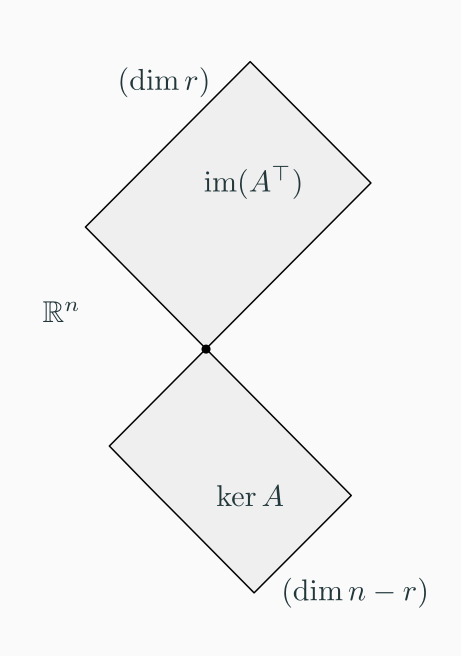
\includegraphics[scale=0.3]{./pics/alg/orthogonal-complements.jpg}
\end{center}

\subsection{QR decomposition theorem}
\label{sec:org2056a2a}
Every matrix \(A \in \mathbb{R}^{m \times n}\) with \emph{linearly independent columns} can be uniquely factorized as $$A = QR,$$ in which the columns of \(Q \in \mathbb{R}^{m \times n}\) are an orthonormal basis for \(\mbox{im }A\) and \(R\in\mathbb{R}^{n \times n}\) is an upper\--triangular matrix with positive entries on the diagonal.
\subsection{Eigenvalues and eigenvectors}
\label{sec:orga19cc1a}
Given a square matrix \(A\in\mathbb{R}^{n \times n}\), \(\lambda \in \mathbb{C}\) is an \textbf{eigenvalue} of \(A\) and \(\nu \in \mathbb{C}^n\) is the corresponding \textbf{eigenvector} if $$A\nu = \lambda\nu, \nu\neq 0,$$ with \((\nu, \lambda)\) \textbf{eigenpair}. Multiplying \(A\) by one of its eigenvectors \(\nu\) results in the very same vector \(\nu\), multiplied by the eigenvalue \(\lambda\). Rewriting the above equation as $$(\lambda I - A)\nu = 0$$ results in an equation whose non\--zero solutions exist if and only if the matrix \((\lambda I - A)\) is rank\--deficient (not a full\--rank matrix); that happens if and only if $$\mbox{det}(\lambda I - A) = 0,$$ that also means that the eigenvalues are the roots of the \(n\mbox{-th}\) degree \textbf{characteristic polynomial} $$p(\lambda) = \mbox{det}(\lambda I - A).$$ A \(n\) rows and columns matrix will possess \(n\) eigenvalues \(\lambda_1, \lambda_2, \dots, \lambda_n\).

If \(\lambda_k\) is an eigenvalue, the set of corresponding eigenvectors is the set of the non\--zero solutions of $$\mbox{det}(\lambda_k I - A)\nu = 0.$$ The union between such set and \(\{0\}\) is said to be \textbf{eigenspace}.

For any matrix \(A\in\mathbb{R}^{n\times n}\),
\begin{itemize}
\item \(\mbox{tr }A = \sum_{i=1}^n \lambda_i\);
\item \(\mbox{det }A = \prod_{i=1}^n \lambda_i\), a singular matrix has at least an eigenvalue which is equal to zero;
\item the rank of \(A\) is equal to the number of non\--zero eigenvalues of \(A\);
\item if \(A\) is not singular, then \((\nu, \lambda)\) is an eigenpair of \(A\), whilst \((\nu, \frac{1}{\lambda})\) is an eigenpair of \(A^{-1}\);
\item if \(A\) is triangular, its eigenvalues are the entries of the main diagonal;
\item if \(A\) is symmetric, its eigenvalues are real\--valued and its eigenvectors are orthogonal.
\end{itemize}
\subsection{Schur decomposition and diagonalization}
\label{sec:org7a7adfe}
Any matrix \(A\in\mathbb{R}^{n \times n}\) can be expressed as the \textbf{Schur decomposition} $$QUQ^*$$ where \(U\) is upper\--triangular, \(Q\) is an \emph{unitary matrix} (whose inverse is the conjugate transpose \(Q^*\)), and both are complex valued.

Any \emph{symmetric} matrix \(A\in\mathbb{R}^{n \times n}\) having eigenvalues \(\lambda_1,\dots,\lambda_n\) can be expressed as $$A = T\Lambda T^\top, $$ where \(\Lambda = \begin{bmatrix} \lambda_1 & 0 & \cdots & 0 \\ 0 & \lambda_2 & \cdots & 0 \\ 0 & 0 & \cdots & \lambda_n\end{bmatrix}\) and \(T\) is an orthogonal matrix. The columns \(t_i\) of \(T\) are the \emph{eigenvectors} associated to the eigenpair \((t_i, \lambda_i)\).
\section{Quadratic forms}
\label{sec:org39e31f8}
\subsection{Definition}
\label{sec:org2b1b92a}
Given \(A\in\mathbb{R}^{n\times n}\) and \(x\in\mathbb{R}^n\) the scalar value \(x^\top A x\) is called a \textbf{quadratic form} such that

$$x^\top A x = \sum_{i=1}^n x_i(Ax)_i = \sum_{i=1}^n x_i\left(\sum_{j=1}^n a_{ij}x_j\right)_i = \sum_{i=1}^n\sum_{j=1}^n a_{ij}x_i x_j.$$

It can be rewritten as \(x^\top A x = x^\top A^\top x\) for properties of transposition. By rearrangin first and last term, $$x^\top A x = x^\top \underbrace{\left( \frac A 2 + \frac{A^\top}{2} \right)}_{\footnotesize \mbox{symmetric part of } A}x,$$ therefore \emph{only the symmetric part contributes to the quadratic form}.
\subsection{Positive definite and semidefinite}
\label{sec:org4e1064b}
A \textbf{positive definite} matrix \(A\in\mathbb{R}^{n \times n}\) is a matrix denoted as \(A \succ 0\) such that $$x^\top A x > 0, \forall x\in\mathbb{R}^n, x \neq 0.$$

A \textbf{positive semidefinite} matrix \(A\in\mathbb{R}^{n \times n}\) is a matrix denoted as \(A \succeq 0\) such that $$x^\top A x \geq 0, \forall x\in\mathbb{R}^n.$$

A \textbf{negative definite} matrix \(A\in\mathbb{R}^{n \times n}\) is a matrix denoted as \(A \prec 0\) such that $$x^\top A x < 0, \forall x\in\mathbb{R}^n, x \neq 0.$$

A \textbf{negative semi semidefinite} matrix \(A\in\mathbb{R}^{n \times n}\) is a matrix denoted as \(A \preceq 0\) such that $$x^\top A x \leq 0, \forall x\in\mathbb{R}^n.$$

Since all eigenvalues of a symmetric matrix \(A\) are real, the following lemmas are useful.

\textbf{Lemma 1} A symmetric matrix \(A\) is positive (negative) definite if and only if all its eigenvalues \(\lambda_i\) are strictly positive (strictly negative), $$A \succ (\prec) 0 \Longrightarrow \lambda_i > (<) 0, i=1,\dots,n.$$

\textbf{Lemma 2} A symmetric matrix \(A\) is positive (negative) semidefinite if and only if all its eigenvalues \(\lambda_i\) are positive (negative), $$A \succeq (\preceq) 0 \Longrightarrow \lambda_i \geq (\leq) 0, i=1,\dots,n.$$

For any squared matrix \(A\), the matrices \((A^\top A)\) and \((AA^\top)\) are both positive semidefinite. For non symmetric matrices, the eigenvalue check should be carried out on their symmetric part.
\subsection{Gradient and Hessian matrix of a quadratic form}
\label{sec:orgeae4cfe}
For any symmetric \(A\in\mathbb{R}^{n\times n}\) matrix,
\begin{itemize}
\item the \textbf{gradient} of a quadratic form (as a column vector) is $$\nabla x^\top A x = 2Ax;$$
\item the \textbf{Hessian matrix} of a quadratic form is $$H(x^\top A x) = 2A.$$
\end{itemize}

\subsection{Cholesky theorem}
\label{sec:org770a271}
Any real symmetric and positive definite matrix \(A\) can be decomposed uniquely as the product of a lower triangular matrix having strictly positive eigenvalues and its transpose, that is $$A = LL^\top,$$ with \(L\) lower triangular having strictly positive eigenvalues (entries on the diagonal that are strictly positive).
\section{Principal Component Analysis}
\label{sec:org6d9d72c}
The \textbf{Principal Component Analysis} (\textbf{PCA}) is an important application of the Schur diagonalization. PCA has many different motivations and interpretations -- among which, one of the most common is \emph{to find the direction along with data varies the most}.

\begin{center}
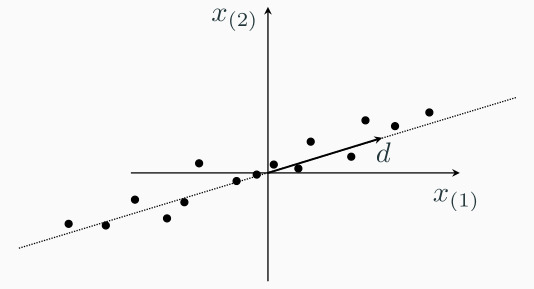
\includegraphics[scale=0.3]{./pics/alg/pca1.jpg}
\end{center}

Let \(n\) points \(x_1, \dots, x_n \in \mathbb{R}^m\) and suppose their mean is zero\footnote{Otherwise, one could subtract $\overline x$ from all vectors.}, $$\overline x \doteq \frac 1 n \sum_{i=1}^n x_i = 0.$$ The component of \(x_i\) along the direction \(d\in\mathbb{R}^m\) is given by the dot product \(d^\top x_i\); the \emph{amount of variation of the data set along direction \(d\)} is then the empirical variance of the components $$\frac 1 n \sum_{i=1}^n \left(d^\top x_i\right)^2.$$

To find the direction of maximal variance, one has to solve

$$\mbox{arg}\max_{||d||_2 = 1} \sum_{i=1}^n \left(d^\top x_i\right)^2 = \mbox{arg}\max_{||d||_2=1} \sum_{i=1}^n \left(d^\top x_i\right)\left(x_i^\top d\right),$$ where the division by \(n\) could be removed as the maximizer is the same.

Collecting all data in a single matrix \(X = \begin{bmatrix}x_1 & \cdots & x_n\end{bmatrix}\) one has that \(d^\top X =\begin{bmatrix}d^\top x_1 & \cdots & d^\top x_n\end{bmatrix}\) and \(X^\top d = \begin{bmatrix}x_1^\top d \\ \vdots \\ x_n^\top d\end{bmatrix},\) hence one can rewrite $$\mbox{arg}\max_{||d||_2=1} d^\top XX^\top d,$$ a more compact form.

The matrix \(XX^\top\) is called the \textbf{covariance matrix}, a symmetric and positive semidefinite matrix by construction. According to Schur diagonalization theorem it can be diagonalized as an orthogonal transform $$XX^\top = T\Lambda T^\top = T\begin{bmatrix} \lambda_1 & 0 & \cdots & 0 \\ 0 & \lambda_2 & \cdots & 0 \\ 0 & 0 & \cdots & \lambda_m\end{bmatrix}T^\top.$$ Each eigenvalue will have a lower value as we run through the diagonal, that is \(\lambda_1 \geq \lambda_2 \geq \dots \geq \lambda_m \geq 0\). The new objective function becomes $$d^\top T\Lambda T^\top d,$$ searching for the maximizing unit vector \(d\). By letting \(y = T^\top d\), and since \(T\) is orthogonal \(||y||_2 = 0 \iff ||d||_2=0\) the problem becomes $$\mbox{arg}\max_{||y||_2=0} y^\top \Lambda y.$$ Since the eigenvalues appear in decreasing order, the \emph{solution} of the above problem is $$y = \begin{bmatrix} 1 & 0 & \dots & 0 \end{bmatrix}^\top.$$ The maximizing \(d\) is, therefore, $$d = Ty = t_1,$$ which is the first column of \(t_1\), corresponding to the eigenvector associated with the \emph{largest eigenvalue} of the covariance matrix.

\begin{center}
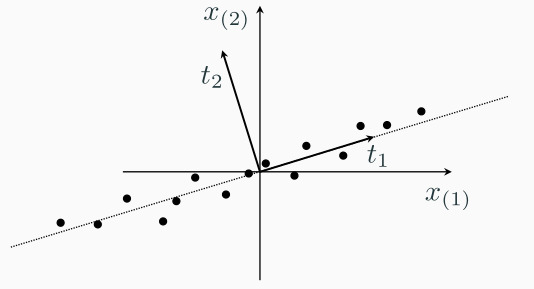
\includegraphics[scale=0.3]{./pics/alg/pca2.jpg}
\end{center}

From the above formulation, it is clear that also the subsequent \(t_2, t_3, \dots, t_m\) represent directions orthogonal to each other that show subsequently decreasing variance, as in Figure.

The PCA can be also used for \emph{dimensionality reduction}. In particular, by projecting the original data in the subspace spanned by the first \(k < m\) columns of \(T\), one can actually reduce the number of dimensions required to describe each example. In practice, this is done picking any original vector \(x \in \mathbb{R}^m\) and projecting it onto the subspace \(\mathcal T\) spanned by vectors \(\{t_1, t_2, \dots, t_m\}\) that were solutions of the previous eigenvalue problem, by means of the matrix \(D = \begin{bmatrix}t_1 & t_2& \cdots & t_m\end{bmatrix}\). The obtained vector \(\hat x \in \mathbb{R}^m\) is \[\hat x = DD^\top x.\] The crucial aspect is that the coordinates of \(\hat x\) with respect to the basis of \(\mathcal T\) (the set of \(t_i\)) are given by $$z = D^\top x,$$ and are called the \textbf{first \(\bf k\) principal components} of \(x\).

\begin{center}
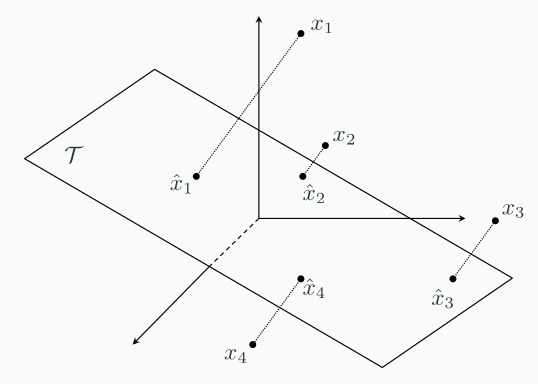
\includegraphics[scale=0.3]{./pics/alg/pca3.jpg}
\end{center}
\chapter{Solution to linear systems of equations}
\label{sec:org108c897}
\section{Exact solutions}
\label{sec:orgdaa8e2f}
\subsection{Homogeneous linear systems}
\label{sec:orga4ef366}
Let the following linear system of equations $$Ax = b$$ where \(A \in\mathbb{R}^{m\times n}\), \(x\in\mathbb{R}^n\) and \(b\in\mathbb{R}^m\). If \(b=0\) the system is said to be \emph{homoegeneous}, $$Ax=0.$$ From the definition of nullspace, the solution is then the \(\mbox{ker }A\). Two cases regarding the rank of the matrix are possible,
\begin{enumerate}
\item the \(\mbox{rank }A = n\), or \(A\) is a full\--column rank matrix. In this case, by the rank\--nullity theorem, \(\mbox{dim}(\mbox{ker }A) = 0\). It follows that \(\mbox{ker }A = \{0\}\) and the only solution is the trivial solution \(x = 0\);
\item the matrix \(A\) is not a full\--rank matrix, that is when \(\mbox{rank }A < n\). In that case, there exist infinite solutions, and the set of solutions is the subspace of \(\mathbb{R}^n\) of dimension $$\mbox{dim}(\mbox{ker }A) = n - \mbox{rank }A \geq 1.$$
\end{enumerate}
\subsection{Non\--homogeneous linear systems}
\label{sec:org2b5ded1}
If \(b \neq 0\), the system is said to be \emph{non\--homogeneous}.

\textbf{Theorem} Consider the system $$Ax = b$$ where \(A \in\mathbb{R}^{m\times n}\), \(x\in\mathbb{R}^n\) and \(b\in\mathbb{R}^m\); the system admits solution if and only if $$\mbox{rank }A = \mbox{rank }\left(\begin{bmatrix} A & b \end{bmatrix}\right).$$ If the system admits solution \(\overline x\), then $$ \overline{\mathcal{X}} = \{x:x = x_0 + \overline x \mbox{ where } x_0 \in \mbox{ker }A\}$$ is the entire space of the solutions.

The following observations are worth to be done,
\begin{itemize}
\item \(\mbox{rank }A = \mbox{rank }\left(\begin{bmatrix} A & b \end{bmatrix}\right)\) is equivalent to state that \(b \in \mbox{im }A\);
\item if \(\mbox{rank }A = n\) and the system admits a solution, then the solution is unique;
\item if \(A\) is a squared, full\--rank matrix the condition is certainly satisfied and there exists a unique solution, which can be found as \(x = A^{-1}b\);
\item the set of solutions is a \emph{linear variety}, as represented in Figure.
\end{itemize}

\begin{center}
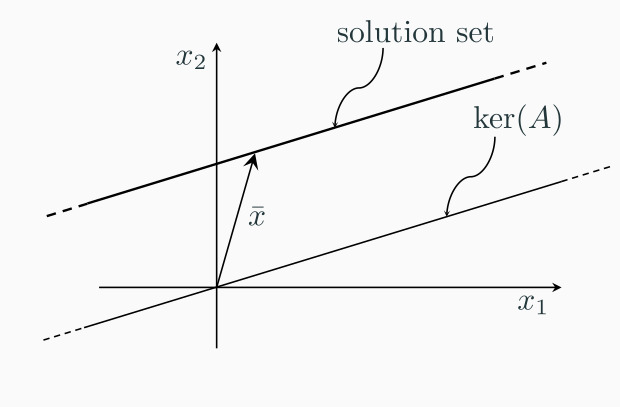
\includegraphics[scale=0.3]{./pics/alg/lssolker.jpg}
\end{center}

\vspace*{0.6cm}\hrule
\hrule
\hrule
\vspace*{0.4cm}


\textbf{Property} For any \(A \in \mathbb{R}^{m \times n}\) it is that $$\mbox{rank }A = \mbox{rank}(A^\top A) = \mbox{rank}(AA^\top).$$

\textbf{Proof} Let's prove the first equality. Let \(x \in \mbox{ker}(A^\top A)\); then \((A^\top A)=0\), and multiplying it by \(x^\top\) to the left one gets \(x^\top A^\top A x = 0\), which means that \(||Ax|| = 0\), hence \(x \in \mbox{ker }A\) belongs to the nullspace. This means that $$x \in \mbox{ker}(A^\top A) \Leftrightarrow x \in \mbox{ker }A,$$ as the other way around is obvious. The second equality follows as \(\mbox{rank }M = \mbox{rank }M^\top\).

\begin{flushright}
$\blacksquare$
\end{flushright}

\vspace*{0.6cm}\hrule
\hrule
\hrule
\vspace*{0.4cm}


In other words, \(A^\top A\) and \(A\) possess the same nullspace, and since they have the same number \(n\) of columns this also means that for the rank\--nullity theorem the dimension of their columnspace must be the same.

\section{Least\--squares approximate solution to overdetermined systems}
\label{sec:orgf26a67a}
In the attempt of fitting a model with real and noisy data, \textbf{overdetermination} of a system of equations is frequently encountered. Overdetermination is a condition in which the ``height'' of \(A\) and \(b\) is much greater than the height of \(x\) -- one will say that \(A\) is a \emph{tall} matrix. One wants to solve \(Ax = b\) with \(b \notin \mbox{im }A\); since the system does not admit a solution, the best idea is to get the \(x\) so that \(Ax\) is the \emph{closest possible} to \(b\). Measuring the distance with Euclidean norm one gets the problem $$\min_{x} ||Ax - b||^2_2.$$

In most frequent cases, \(A\) is a full\--rank matrix and the problem admits a single solution of the form

\[
\begin{array}{rcl} || Ax - b || ^2_2 & = & (Ax - b)^\top (Ax - b) = (x^\top A^\top - b^\top)(Ax - b) \\ & = & x^\top A^\top A x - 2 x^\top A^\top b + b^\top b;\end{array}\] by taking the gradient with respect to \(x\) and equating to zero to find the solution one gets \[2A^\top A x - 2A^\top b = 0, \mbox{ that is } A^\top A x = A^\top b.\] The matrix \(A^\top A \in \mathbb{R}^{n \times n}\) and its rank is \(n\) (full\--rank matrix). For these reasons \(A^\top A\) is invertible, and one can obtain the closest solution $$\hat x = (A^\top A)^{-1}A^\top b.$$

The geometric interpretation of the least\--squares solution, since \(A\hat x\) is, by definition, the point that is \emph{the closest} to \(b\) while still belonging to \(\mbox{im }A\). This means that \(||A\hat x||\) is the \emph{projection} of \(b\) onto \(\mbox{im }A\).

\begin{center}
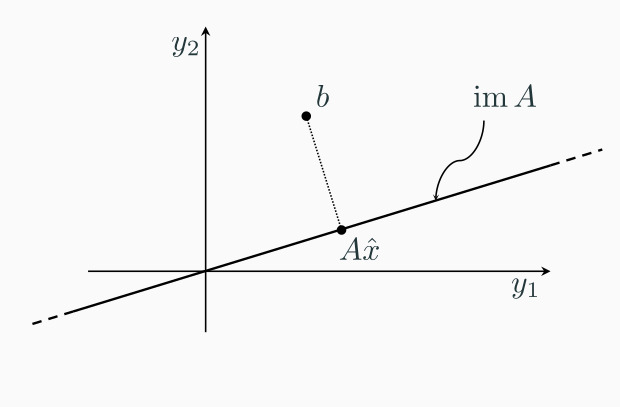
\includegraphics[scale=0.3]{./pics/alg/lsas.jpg}
\end{center}
\section{Minimum\--norm solution to underdetermined systems}
\label{sec:org4714c8f}
Differently from the previous case, \textbf{underdetermined} systems are all systems whose \(x\) is ``taller'' than \(A\) and \(b\), a case that happens when when there are more variables than independent equations. In this case, infinite solutions exists if \(\mbox{rank }A = m\) and \(m > n\). A possible workaround in this case is to find the \emph{minimum\--norm solution} by solving the problem $$\min||x||_2$$ subject to $$Ax = b.$$

The problem can be stated as $$\min x^\top x,$$ with the same constraints. By introducing the \emph{Lagrange multipliers} on \(\lambda \in \mathbb {R}^m\) one can get the problem \[\mathcal{L}(x, \lambda) = x^\top x + \lambda^\top (Ax - b).\] Since this is a problem with a Lagrangian multiplier, to solve it one should impose the \emph{stationary conditions} by computing the gradient for all variables and set the obtained quantities to \(0\),

\[\begin{array}{rcl}
\nabla_x \mathcal{L}(x, \lambda) & = & 2x + A^\top \lambda = 0\\
\nabla_\lambda \mathcal{L}(x, \lambda) & = & Ax - b = 0.
\end{array} \]

From the first, \(x = -A^\top \frac \lambda 2\), and from the second \(\lambda = -2(AA^\top)^{-1}b\), with \(AA^\top \in \mathbb{R}^{m \times m}\) certainly invertible as it is a full\--rank matrix whose rank is \(m\).

The minimum\--norm solution can be then found by substituting the second in the first, that is $$\hat x = A^\top(AA^\top)^{-1}b.$$

\begin{center}
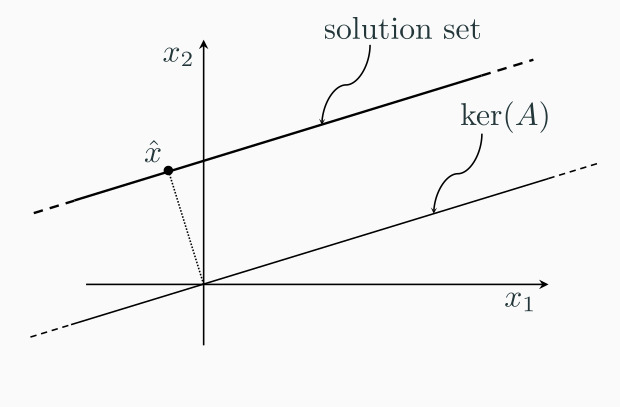
\includegraphics[scale=0.3]{./pics/alg/mns.jpg}
\end{center}

The minimum norm solution is \emph{orthogonal} to \(\mbox{ker }A\), as for any \(\kappa \in \mbox{ker }A\) one has both \(A\kappa = 0\) and \(\kappa^\top A^\top = 0\); thus,
$$\kappa^\top \hat x = \kappa^\top A^\top (AA^\top)^{-1}b = 0.$$

The geometric interpretation for the minimum norm solution is that \(\hat x\) is the \emph{projection} of the origin of \(\mathbb{R}^n\) onto the solution set of \(Ax - b =0\).
\chapter{Singular Value Decomposition}
\label{sec:org49d1cf1}
\section{Theorem of SVD}
\label{sec:org699ee5b}
Any matrix \(A \in \mathbb{R}^{m \times n}\) can be written with the \textbf{Singular Value Decomposition} as $$A = U\Sigma V^\top$$ where \(U \in \mathbb{R}^{m \times m}\) and \(V \in \mathbb{R}^{n \times n}\) are \emph{orthogonal} matrices and \(\Sigma \in \mathbb{R}^{m \times n}\) possesses the form
\[\Sigma = \begin{bmatrix}\Sigma_1 & 0 \\ 0 & 0\end{bmatrix},\] where
\[\Sigma_1 = \begin{bmatrix} \sigma_1 & 0 & \cdots & 0 \\ 0 & \sigma_2 & \cdots & 0 \\ \vdots & \vdots & \ddots & \vdots \\ 0 & \cdots & 0 & \sigma_p\end{bmatrix},\] and $$\sigma_1 \geq \sigma_2 \geq \dots \geq \sigma_p \geq 0, p \leq \min(m,n).$$

The \(\sigma_i\) are called \textbf{singular values} of \(A\), while the \(m\) columns \(u_i\) of \(U\) are called \textbf{left singular vectors} of \(A\), and the \(n\) columns \(v_i\) of \(V\) are said to be \textbf{right singular vectors} of \(A\). For any \(1 \leq i \leq p\) it holds that

$$Av_i = U\Sigma V^\top v_i = U\Sigma \begin{bmatrix}0 \\ \vdots \\ 1 \\ 0 \\ \vdots \\ 0\end{bmatrix} = U\begin{bmatrix}0 \\ \vdots \\ \sigma_i \\ 0 \\ \vdots \\ 0\end{bmatrix} = \sigma_i u_i,$$ and similarly $$A^\top u_i = \sigma_i v_i.$$ Rearranging these equations, $$(A^\top A)v_i = \sigma^2_i v_i, i = 1,\dots, p,$$ therefore \((v_i, \sigma^2_i)\) is an \emph{eigenpair} of \(A^\top A\); the same goes for $$(AA^\top )u_i = \sigma^2_i u_i, i = 1,\dots, p,$$ so \((u_i, \sigma^2_i)\) is \emph{eigenpair} of \(AA^\top\).

\textbf{Property} Let \(A \in \mathbb{R}^{m \times n}\). If \(n \geq m\), the singular values of \(A\) are the square roots of the eigenvalues of \(AA^\top\), else if \(m \geq n\) the singular values of \(A\) are the square roots of the eigenvalues of \(A^\top A\).

\vspace*{0.6cm}\hrule
\hrule
\hrule
\vspace*{0.4cm}


\textbf{Property} The rank of \(A\) equals to the number of non\--zero singular values of \(A\).

\textbf{Proof} Observe that, since \(U\) and \(V^\top\) are not singular and orthogonal, $$\mbox{rank }A = \mbox{rank }(U\Sigma V^\top)= \mbox{rank }\Sigma.$$
\begin{flushright}
$\blacksquare$
\end{flushright}

\vspace*{0.6cm}\hrule
\hrule
\hrule
\vspace*{0.4cm}

\section{Interpretation of SVD}
\label{sec:orga4a5673}
\subsection{SVD to provide bases for the image and the kernel of \(A\)}
\label{sec:orge07c853}
\textbf{Proposition} If \(A = U\Sigma V^\top\) (has a singular value decomposition) and \(\mbox{rank }A = r\), then
\begin{enumerate}
\item the first \(r\) columns of \(U\) are a basis for \(\mbox{im }A\);
\item the last \(n - r\) columns of \(V\) are a basis for \(\mbox{ker }A\).
\end{enumerate}

Moreover, the Frobenius norm and the Euclidean norm can be expressed in terms of singular values, so that

\[\begin{array}{lcl} ||A||^2_F & = &  \sigma^2_1 + \sigma^2_2 + \dots + \sigma^2_p \\ ||A||_2 & = & \sigma_1. \end{array}\]

\begin{center}
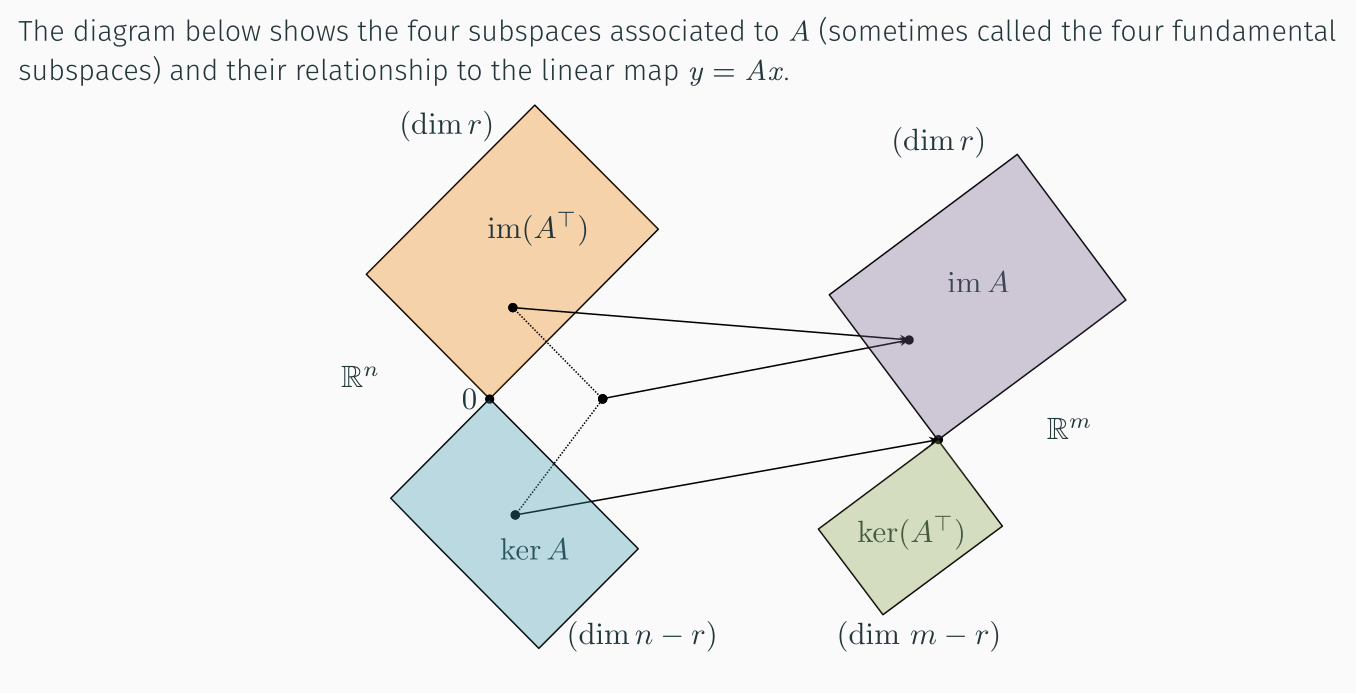
\includegraphics[width=.9\linewidth]{./pics/alg/fundamental-subspaces.jpg}
\end{center}
\begin{center}
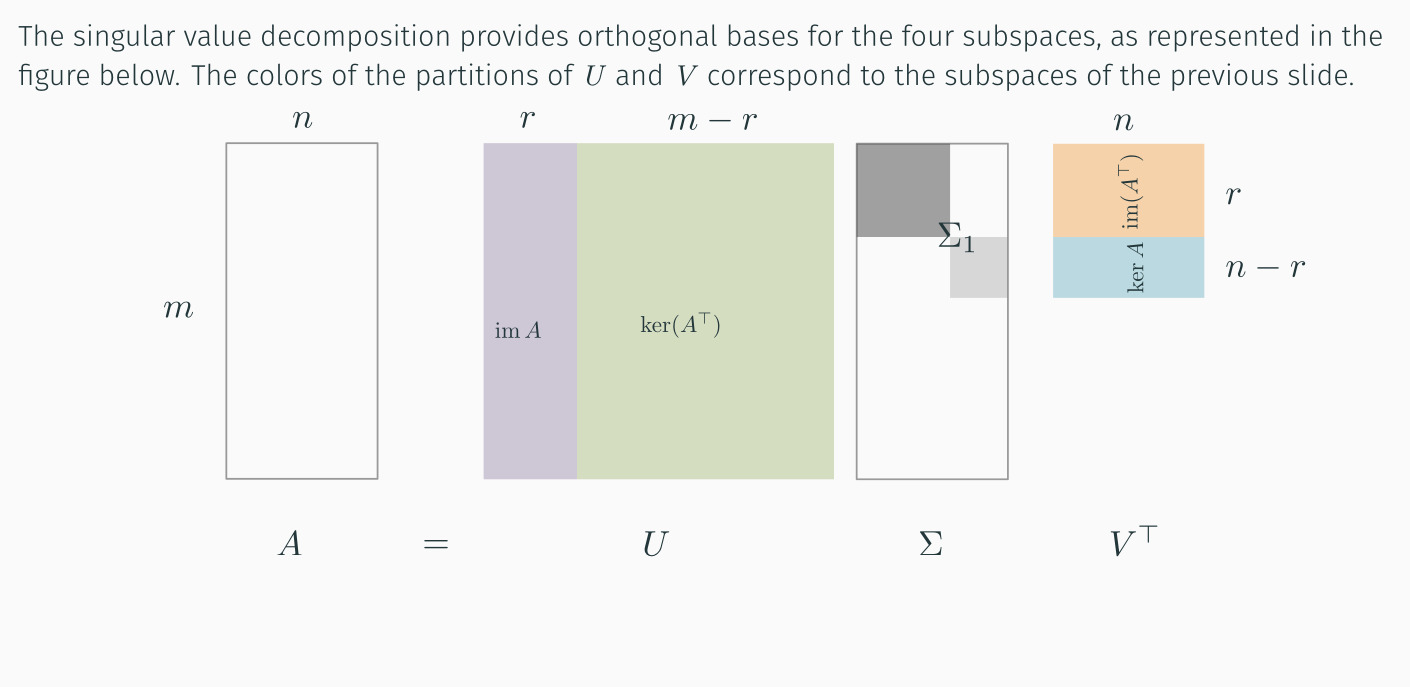
\includegraphics[width=.9\linewidth]{./pics/alg/fundamental-subspaces2.jpg}
\end{center}

\subsection{Geometrical meaning of SVD}
\label{sec:orgb17e21e}
Singular Value Decomposition admits a fundamental geometrical meaning. The singular values of \(A \in \mathbb{R}^{m \times n}\) represent the \emph{length of the semiaxes of the hyperellipse} in \(\mathbb{R}^m\) obtained by applying linear map \(A\) to the unit hypersphere in \(\mathbb{R}^n\), centered at the origin, as in Figure, where it is shown an example concerning \(\mathbb{R}^2\).

\begin{center}
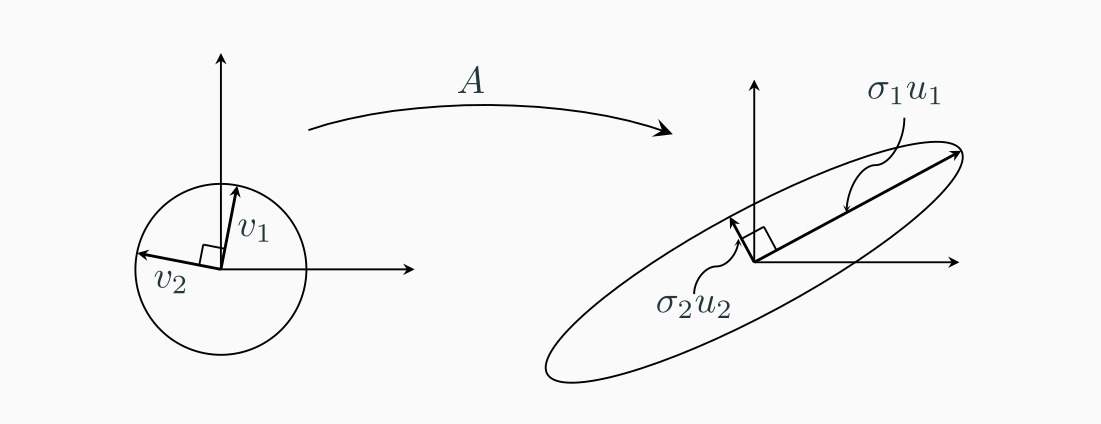
\includegraphics[width=.9\linewidth]{./pics/alg/svd-geom.jpg}
\end{center}

In fact,

\[\begin{array}{rcl} ||Av_1|| & = & ||\sigma_1 u_1|| = \sigma_1 ||u_1|| = \sigma_1\\ ||Av_2|| & = & ||\sigma_2 u_2|| = \sigma_2 ||u_2|| = \sigma_2\end{array}.\]
\subsection{Singular values against eigenvalues}
\label{sec:org7e52d54}

Singular values are different from eigenvalues, as they exist for \emph{any} matrix, while eigenvalues are only possessed by square matrices. Singular values are also \emph{always real} and \emph{always non\--negative}. For a square matrix \(A\), one can compute singular values from eigenvalues in the following way, $$\sigma_i = \sqrt{\lambda_i},$$ with the eigenvalues computed either from \(A^\top A\) or \(AA^\top\).
\section{Compact Singular Value Decomposition and dyadic expansion}
\label{sec:org6fabf77}
\subsection{Compact SVD and dyadic expansion}
\label{sec:org0256baa}
\textbf{Compact SVD} form can be achieved by the following way.

\textbf{Proposition} Let \(A \in \mathbb{R}^{m \times n}\) and \(\mbox{rank }A =r\). If \(A = U\Sigma V^\top\), it is $$A = U_r\Sigma_r V^\top_r,$$ where \(U_r = \begin{bmatrix}u_1 & \cdots  & u_r\end{bmatrix}\), \(V_r = \begin{bmatrix}v_1 & \cdots  & v_r\end{bmatrix}\), and \(\Sigma_r = \mbox{diag }\{\sigma_1, \sigma_2, \dots, \sigma_r\}.\) Moreover, \(A\) admits its \emph{dyadic expansion} such that $$A = \sum_{i=1}^r \sigma_i \underbrace{u_i v^\top_i}_{Z_i} = \sum_{i=1}^r \sigma_i Z_i,$$ with matrices \(Z_i \in \mathbb{R}^{m \times n}\), and \(\mbox{rank }Z_i = 1\).
\subsection{Two theorems for low rank approximation}
\label{sec:org4d92b96}
\textbf{Theorem} Let \(k < r = \mbox{rank }A\) and \(A_{(k)} = \sum_{i=1}^k \sigma_i u_i v^\top_i\). Then, $$\min_{\mbox{\footnotesize rank }B \leq k} ||A-B||_2 = ||A - A_{(k)}||_2 = \sigma_{k+1}.$$

\textbf{Theorem} Let \(k < r = \mbox{rank }A\) and \(A_{(k)} = \sum_{i=1}^k \sigma_i u_i v^\top_i\). Then, $$\min_{\mbox{\footnotesize rank }B \leq k} ||A-B||_F = ||A - A_{(k)}||_F = \sum_{i=k+1}^r \sigma_{i}.$$

Basically, \(A_{(k)}\) is the best approximation of low rank \(k \leq r\) of \(A\), with respect to both Euclidean and Frobenius norm. One can write $$A_{(k)} = U_k \Sigma_k V^\top_k,$$ where \(U_k = \begin{bmatrix}u_1 & \cdots  & u_k\end{bmatrix}\), \(V_k = \begin{bmatrix}v_1 & \cdots  & v_k\end{bmatrix}\), and \(\Sigma_k = \mbox{diag }\{\sigma_1, \sigma_2, \dots, \sigma_k\},\) with only \(k\) entries instead of \(r\). This means that we can use \(k\) singular values only instead of all \(r\) ones to approximate a matrix \(A\).
\section{Solution to problems}
\label{sec:org7283afe}
\subsection{Non\--trivial approximate solutions to linear, homogeneous systems}
\label{sec:org04db35e}
Let \(Ax = 0\) a linear homogeneous system of equations with \(A \in \mathbb{R}^{m \times n}\). The only case where \(A\) doesn't have a trivial \(x=0\) solution is when \(A\) is not full\--rank. Unfortunately, when dealing with noisy data, it almost always happens that \(A\) is a full\--rank matrix. In order to get a non\--trivial solution, the following problem can be solved $$\min_{||x||=1} ||Ax||^2,$$ that is the problem of minimization (closest to zero) of the norm of \(Ax\), provided \(x \neq \bf 0\). The choice of \(||x|| = 1\) is arbitrary, as we are only interested in the direction of \(x\).

\vspace*{0.6cm}\hrule
\hrule
\hrule
\vspace*{0.4cm}
\textbf{Theorem} Let \(A\in\mathbb{R}^{m \times n}\) and \(Ax = 0\) a linear, homogeneous system of equations. The solution of constrained minimization problem $$\min_{||x||=1} ||Ax||^2$$ is \(\hat x = v_n\), with \(v_n\) being the \(n\mbox{-th}\) column of \(V\), the right singular vector associated to the \emph{smallest} singular value.

\textbf{Proof} Recalling that \(U\) and \(V\) are orthogonal, it follows that
$$\begin{array}{rcl} \min_{||x||=1} ||Ax||^2 & = & \min_{||x||=1} ||U\Sigma V^\top x||^2  = \min_{||x||=1} ||\Sigma V^\top x||^2 = \min_{||y||=1}||\Sigma y||^2 \\ & = & \min_{||y||=1} \sum_{i}\sigma^2_i y_i.\end{array}$$

As the singular values appear in decreasing order, the solution is \(y = \begin{bmatrix}0 \\ 0 \\ \vdots \\ 1\end{bmatrix}\), therefore \(\hat x = v_n\).

\begin{flushright}
$\blacksquare$
\end{flushright}

\vspace*{0.6cm}\hrule
\hrule
\hrule
\vspace*{0.4cm}
\subsection{Orthogonal Procrustes problem}
\label{sec:org7a1a256}

The \textbf{Orthogonal Procrustes problem} amounts to finding the orthogonal transformation \(W\) that renders the transformed matrix \(WB\) as close as possible to \(A\) in Frobenius norm.

\textbf{Theorem (Orthogonal Procrustes problem)} Given \(A\) and \(B\) matrices, the solution to $$\min_{W^\top W=I} ||A - WB||^2_F$$ is \(W=VU^\top\), where \(BA^\top = U\Sigma V^\top\) is the singular value decomposition of \(BA^\top\).

A special case is when \(B = I\), with the goal of finding \(W\) closest to \(A\). Hence,
$$\min_{W^\top W=I} ||A - W||^2_F,$$ whose solution is \(W = VU^\top\) but with \(IA^\top = A^\top = U\Sigma V^\top\).
\subsection{PCA and SVD}
\label{sec:orgd342027}
Principal Component Analysis of a matrix \(X\) corresponds to the eigenvalue decomposition of the symmetric and positive semidefinite matrix \(XX^\top\), such that \(XX^\top = T\Lambda T^\top\). Considering now the SVD of \(X = U\Sigma V^\top\), one obtains

$$XX^\top = \left(U\Sigma V^\top\right)\left(U\Sigma V^\top\right)^\top = U\Sigma \underbrace{V^\top V}_{I} \Sigma^\top U^\top = U\Sigma^2 U^\top.$$ But, since \(\Sigma\) is diagonal, \(\Sigma^2\) is diagonal as well and it corresponds to an eigenvalue decomposition as in the original PCA computation and the columns \(u_i\) of \(U\) are indeed the eigenvectors of \(XX^\top\) associated with the eigenvalues \(\lambda_i =\sigma^2_i\). This basically means that \(U = T\) and \(\Lambda = \Sigma^2\). The Principal Component Analysis reduces to computing the Singular Value Decomposition for \(X\) \emph{without computing the matrix} \(XX^\top\), then performing the square of the singular values.

By denoting \(U_k\) the matrix containing the first \(k\) columns of \(U\), one can state that the vector containing the first \(k\) principal components of \(x\) is indeed \(U^\top_k x\).
\subsection{Dimensionality reduction with SVD}
\label{sec:orgc0bc744}
Suppose \(n\) points are given in \(\mathbb{R}^m\). One can build the matrix \(X\) as $$X = \begin{bmatrix}x_1 & x_2 & \cdots & x_n\end{bmatrix} \in \mathbb{R}^{m \times n}.$$ Let now \(D\) be an orthornormal basis for a subspace \(\mathcal D\) of \(\mathbb{R}^m\), $$D = \begin{bmatrix} d_1 & d_2 & \cdots & d_k\end{bmatrix},$$ with \(k < n\). The projection of \(x\) onto \(\mathcal D\) is $$\hat x = DD^\top x.$$

\begin{center}
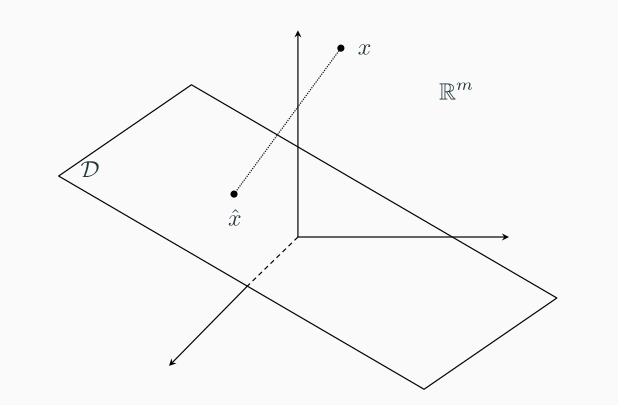
\includegraphics[scale=0.3]{./pics/alg/proj-d.jpg}
\end{center}

The dimensionality of the set of vectors can be reduced by encoding each \(x_i\) as a vector \(z_i \in \mathbb{R}^k\) of the components of \(\hat {x}_i\) along the basis given by the columns of \(D\), $$z_i = D^\top x_i.$$

Reconstruction of the vector can be performed by simply \(\hat {x}_i = Dz_i \in \mathbb{R}^m.\) For a given \(k < m\) \emph{target dimensionality} a reasonable criterion for the choice of \(D\) is the \emph{minimization of the sum of the squared reconstruction errors}, that is
$$D_{opt} = \mbox{arg} \min_{D^\top D = I} \sum_{i=1}^n ||x_i - \underbrace{DD^\top x_i}_{\hat x_i}||^2_2,$$ with the constraint that guarantees that all columns of \(D\) form a orthonormal basis.

Rewriting the same, but employing Frobenius norm, one can jot down the corresponding compact form
$$D_{opt} = \mbox{arg} \min_{D^\top D = I} \sum_{i=1}^n ||X - \underbrace{DD^\top X}_{\doteq \hat B}||^2_F.$$

As \(\mbox{rank }D = k\), one has that \(\mbox{rank }B \leq k\); for this reason, the problem expressed in Frobenius norm can be seen as a constrained, low\--rank approximation problem (the constraint is on \(B\), which must be of the form \(DD^\top X\) with \(D\) of orthogonal, unit norm, columns). Since we are in front of a low\--rank approximation problem, the solution of the \emph{unconstrained} problem is $$B = U_k\Sigma_k V^\top_k.$$

\vspace*{0.6cm}\hrule
\hrule
\hrule
\vspace*{0.4cm}
\textbf{Preposition} \(B = U_k\Sigma_k V^\top_k\) also satisfied the constrained problem, for \(B\) of the form \(DD^\top X\) with \(D\) having orthonormal columns, with \(D = U_k\).

\textbf{Proof} Let's decompose to the singular values \(X = U\Sigma V^\top\). Let's denote \(\bigstar\) any submatrix that doesn't affect the result in any way (as the term is multiplied by zero, thus canceled).

One then has

\[\begin{array}{rcl} U_k U^\top_k X & = & U_k U^\top_k U \Sigma V^\top \\ & = & U_k \begin{bmatrix}I_k & 0 \end{bmatrix}\begin{bmatrix}\Sigma_k & 0 \\ 0 & \bigstar \end{bmatrix}\begin{bmatrix}V^\top_k \\ \bigstar \end{bmatrix} \\ & = & U_k\begin{bmatrix}\Sigma_k & 0 \end{bmatrix}\begin{bmatrix}V^\top_k \\ \bigstar \end{bmatrix} \\ & = & U_k \Sigma_k V^\top_k. \end{array}\]

\begin{flushright}
$\blacksquare$
\end{flushright}

\vspace*{0.6cm}\hrule
\hrule
\hrule
\vspace*{0.4cm}
\chapter{Rigid Geometric Transforms}
\label{sec:orgbad3ad1}
\section{Reference systems}
\label{sec:org1cbb686}
\subsection{Cartesian reference system}
\label{sec:org5cbb158}
A \textbf{Cartesian reference system} for three\--dimensional space consists of a point called \emph{origin} and three mutually perpendicular oriented lines through the origin, called \emph{axes}. The order in which the axes are listed \((x, y, z)\) is fixed and is a part of the definition itself. Three planes exist -- the plane perpendicular to the first axis \(x\) is the \emph{first reference plane}. Positive directions of the axes are typically marked by specific points at distance \(1\) from the origin. These points are called the \emph{unit points}. A Cartesian reference system is said to be \emph{right\--handed} if the smallest rotation that brings the first unit point to the second unit point is counterclockwise, as viewed from the third unit point. It is \emph{left\--handed} if otherwise. The vectors \(e_x\), \(e_y\) and \(e_z\) specify the unit points and lie on the axes, respectively, \(x\), \(y\) and \(z\).
\subsection{Cartesian coordinates}
\label{sec:orgf15f9f7}
\textbf{Cartesian coordinates} are the \emph{signed distances} of the point from the first, second and third reference plane. The sign of the \(i\mbox{-th}\) coordinate is positive whether it belongs to the the half\--space delimited by the \(i\mbox{-th}\) reference plane containing the \(i\mbox{-th}\) point.

It follows that
\begin{itemize}
\item coordinates of the origin are vector \(t = \begin{bmatrix} 0 & 0 & 0 \end{bmatrix}^\top\);
\item coordinates of the unit points are \(e_x = \begin{bmatrix} 1 \\ 0 \\ 0\end{bmatrix}\), \(e_y = \begin{bmatrix} 0 \\ 1 \\ 0\end{bmatrix}\) and \(e_z = \begin{bmatrix} 0 \\ 0 \\ 1\end{bmatrix}\);
\item the vector \(p = \begin{bmatrix}x \\ y \\ z\end{bmatrix}\), coordinates of a generic point \(P\) in space, can be written as $$p = xe_x + ye_y + ze_z;$$
\item applying Pytagorean theorem, the distance from the origin \(O\) is $$d(O, P) = \sqrt{x^2 + y^2 + z^2} = ||p||_2.$$
\end{itemize}
\subsection{Orthogonal projection}
\label{sec:orge3f5834}
Given two vectors \(a\) and \(b\), the \textbf{orthogonal projection} of \(a\) onto \(b\) is the vector \(p \in \mbox{span }\{b\}\) that is \emph{the closest to} \(a\):

$$p = \mbox{arg}\min_{p\in\mbox{\footnotesize span}\{b\}} ||p - a||.$$ In Figure,

\begin{center}
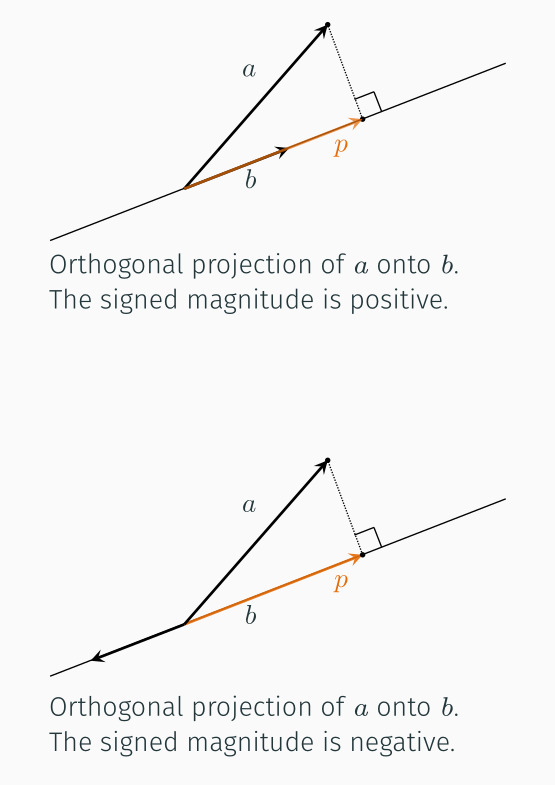
\includegraphics[scale=0.3]{./pics/alg/orth-proj.jpg}
\end{center}

Projection \(p\) can also be obtained via a suitable \emph{projection matrix} \(P_b\), that is $$p = P_b a,$$ where \(P_b\) is the following square symmetric matrix having rank \(1\) $$P_b = \frac{bb^\top}{b^\top b} = \frac{bb^\top}{||b||^2}.$$

Orthogonal projection has its own sign. The \emph{signed magnitude} of the orthogonal projection is $$\tilde p = \frac{b^\top a}{||b||} =||p||\mbox{sign}(b^\top a).$$

\textbf{Property} The coordinates of a point in space are the signed magnitudes of the orthogonal projections of the vector of coordinates of the point onto the three unit vectors that define the coordinate axes.
\subsection{Multiple reference systems}
\label{sec:org6f4e962}
\textbf{Multiple reference systems} can be introduced. To avoid confusion, notation will be clarified now:
\begin{itemize}
\item reference systems are identified as natural numbers -- to each of them, a natural number label will be assigned;
\item the reference system whose number is \(0\) is said to be the \textbf{world reference frame};
\item a left superscript will be used to denote the reference system a vector belongs to;
\item left superscript of zero might be omitted for brevity;
\item the origin will be denoted as \({}^{i}t_i\) for all \(i\);
\item unit vectors for \(q\mbox{-th}\) reference system will be denoted as \({}^qi_q\), \({}^qj_q\) and \({}^qk_q\), and for each \(q\mbox{-th}\) reference system, $$\begin{bmatrix} {}^qi_q & {}^qj_q & {}^qk_q \end{bmatrix} = \begin{bmatrix} i_0 & j_0 & k_0 \end{bmatrix} = \begin{bmatrix} 1 & 0 & 0 \\ 0 & 1 & 0 \\ 0 & 0 & 1 \end{bmatrix} = I.$$
\end{itemize}
\section{Rotations}
\label{sec:org2e9601f}

\subsection{Definition}
\label{sec:org0ad8ebe}

A \textbf{rotation} is a transformation between two Cartesian reference systems \(S_0\) and \(S_1\) of equal origin \(t_0 = t_1 = \begin{bmatrix}0 \\ 0 \\ 0 \end{bmatrix}\) and handedness.

\begin{center}
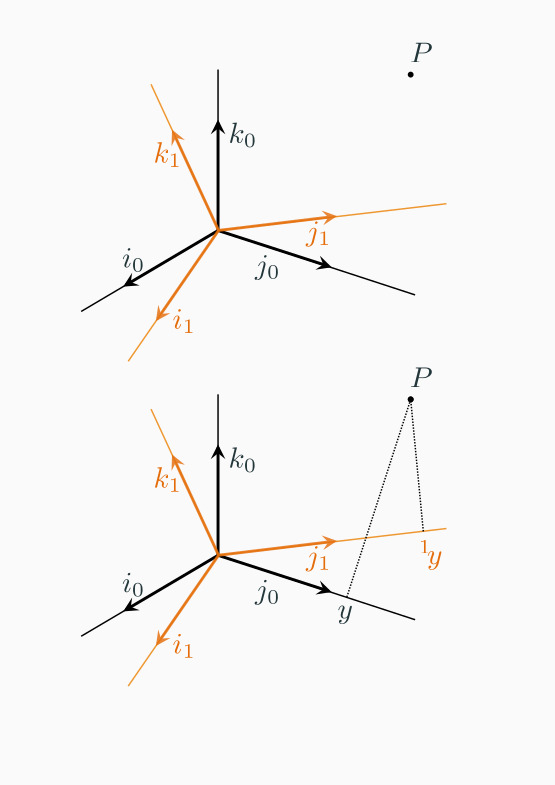
\includegraphics[scale=0.3]{./pics/alg/rotation.jpg}
\end{center}

One has that a point \(P\) can be expressed as \[p = \begin{bmatrix} x \\ y \\ z\end{bmatrix} = xi_0 + yj_0 + zk_0;\] in \(S_1\) the very same triplet is \[p = {}^1 xi_1 + {}^1 yj_1 + {}^1 zk_1,\] with \({}^1x\), \({}^1y\) and \({}^1z\) the orthogonal projections of \(p\) onto \(i_1\), \(j_1\) and \(k_1\) respectively. That is $${}^1x = i^\top_1 p, \hspace{1cm}{}^1y = j^\top_1 p, \hspace{1cm}{}^1z = k^\top_1 p.$$ If one defines \({}^1 p = \begin{bmatrix} {}^1 x & {}^1 y & {}^1 z\end{bmatrix}^\top\), he can reach a compact form \({}^1 p = R_1 p\), where $$R_1 = {}^0R_1 = \begin{bmatrix}i^\top_1 \\ j^\top_1 \\ k^\top_1\end{bmatrix},$$ with \({}^0R_1\) being a \(3 \times 3\) \textbf{rotation matrix}.

In general, given any two Cartesian reference systems \(S_a\) and \(S_b\) sharing the same origin, any point $${}^bp = {}^aR_b {}^a p, \mbox{ where } {}^aR_b = \begin{bmatrix} {}^a i^\top_b &  {}^a j^\top_b &  {}^a k^\top_b \end{bmatrix}.$$ Vector \({}^b p\) expressed in corodinates of system \(S_b\) can be obtained by left\--multiplying by \({}^aR_b\) the vector \({}^a p\) expressed in coordinates of system \(S_a\). Finally, the rows of \({}^a R_b\) are the coordinates of unit points of \(S_b\) expressed in the reference \(S_a\), so that the transformations occurs.

If a rotation is obtained by rotating \(S_0\) about its third axis \(z\), one can express \[{}^0 R_1(\theta) = \begin{bmatrix} \cos \theta & \sin \theta & 0 \\ -\sin \theta & \cos\theta & 0 \\ 0 & 0 & 1\end{bmatrix},\] with the third row being different, so that the third coordinate \(z\) remains unchanged.
\subsection{Inverse rotation}
\label{sec:org670ffc4}

As the rotation is a reversible transformation, it means that its inverse must exist. Indeed, its inverse is such that $${}^a p = {}^b R_a {}^b p.$$ By applying previous transformation on this equation, one gets

$${}^a p = {}^b R_a ({}^a R_b {}^a p) =\underbrace{{}^b R_a {}^a R_b}_{I} {}^a p.$$

\textbf{Theorem} The inverse of a rotation matrix \(R\) is its transpose \(R^{-1} = R^\top\), hence $$R^\top R = RR^\top = I.$$

For this reason, \(R\) is an \emph{orthogonal} matrix (its columns are mutually orthogonal and unitary, as well as its rows). Orthogonal matrices can have determinant either equal to \(1\) or equal to \(-1\). An orthogonal matrix \emph{is not} a rotation matrix if its determinant is equal to \(-1\), as it would correspond to an \emph{inversion} -- also called \emph{mirror flip} -- of the axes. Basically, it would correspond to a rotation \emph{plus} an inversion of the third axis.

\textbf{Lemma} A matrix \(R\) is a rotation matrix if and only if \(R^\top R= RR^\top = I\) and \(\mbox{det }R = 1\).

Hence, being orthogonal is not a sufficient condition for being a rotation matrix, as the determinant of a rotation matrix should be equal to \(1\). Figure shows a transformation performed with an orthogonal matrix whose determinant is equal to \(-1\),

\begin{center}
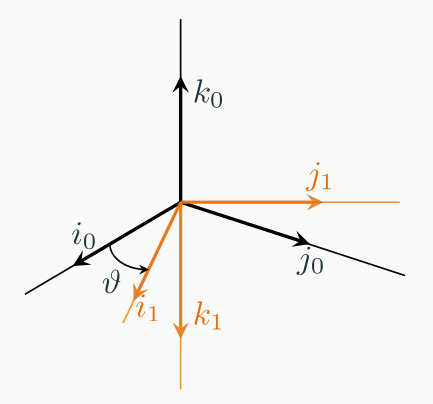
\includegraphics[scale=0.3]{./pics/alg/neg-rot.jpg}
\end{center}
\clearpage
\section{Coordinate transformations}
\label{sec:org03af325}
\subsection{Translation and rotation}
\label{sec:org3500019}
Given \(S_0\) world reference frame, a new reference frame \(S_1\) can differ from \(S_0\) by a translation of the origin from \(t_0\) to \(t_1\) and a rotation of the axes from \(i_0, j_0, k_0\) to \(i_1, j_1, k_1\). A point \(P\) whose coordinates \(p = \begin{bmatrix}x \\ y \\ z\end{bmatrix}\) will end up having coordinates \({}^1 p = \begin{bmatrix}{}^1 x \\ {}^1 y \\ {}^1 z\end{bmatrix}\) on the reference system \(S_1\).

Let's divide the entire transformation into two distinct transformations:
\begin{enumerate}
\item the first involves the origin of \(S_0\) to be translated from \(t_0\) to \(t_1\) by performing a \emph{translation}. The new coordinates for the point are \(p - t_1\);
\item the second involves a rotation of the axis so that they are properly rotated. The rotation is described by the rotation matrix \(R_1\).
\end{enumerate}

\begin{center}
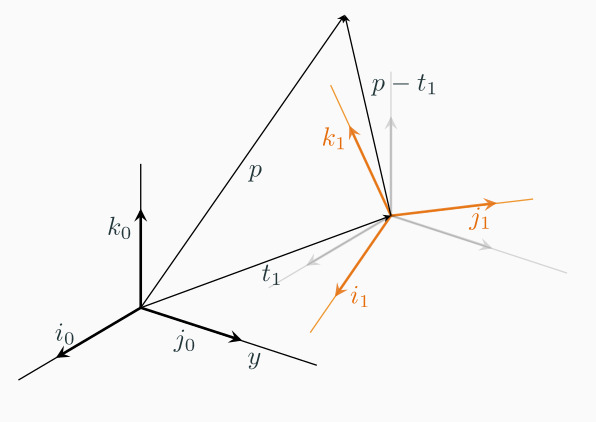
\includegraphics[scale=0.3]{./pics/alg/rot-transl.jpg}
\end{center}

The coordinates in \(S_1\) are thus expressed as $${}^1 p = R_1(p - t_1).$$ Indeed, solving for \(p\) yields the inverse transformation $$p = R^\top_1 {}^1 p + t_1,$$ corresponding to a rotation of \(R^\top_1\), followed by a translation of the quantity \(-t_1\). It can be rewritten as $$p = R^\top_1 ({}^1 p - (-R_1 t_1)),$$ and by comparing the previous ones it follows that $${}^1 R_0 = {}^0 R^\top_1, \hspace*{1cm} \mbox{and} \hspace*{1cm} {}^1 t_0 = -{}^0 R_1 {}^0 t_1.$$

More generally, if \({}^b p = {}^aR_b({}^a p - {}^at_b)\), it follows that

$${}^a p =  {}^bR_a ({}^b p - {}^b t_a),$$ where
$${}^b R_a = {}^a R^\top_b, \hspace*{1cm} \mbox{and} \hspace*{1cm} {}^b t_a = -{}^a R_b {}^a t_b.$$

\subsection{Homogeneous transformations}
\label{sec:org84e2e34}
Consider \({}^b p = {}^aR_b({}^a p - {}^at_b)\). A compact representation of the coordinate transform can be obtained by rearranging terms in such way,

\[\begin{array}{rcl} {}^b p = {}^a R_b ({}^a p - {}^a t_b) & = & {}^a R_b {}^a p - {}^a R_b {}^a t_b \\ & = & \begin{bmatrix} \underbrace{{}^a R_b}_{3 \times 3} & \underbrace{-{}^a R_b{}^a t_b}_{3 \times 1}\end{bmatrix}\begin{bmatrix}{}^a p \\ 1\end{bmatrix}. \end{array}\]

One can interpret this result as first \emph{rotating} and then \emph{translating} -- with the translated vector expressed with respect to the intermediate, rotated reference system. Indeed,

\[\begin{bmatrix}{}^b p \\ 1\end{bmatrix} = \begin{bmatrix} {}^a R_b & - {}^a R_b {}^a t_b \\ 0^\top & 1 \end{bmatrix}\begin{bmatrix} {}^a p \\ 1\end{bmatrix}.\]

Homogeneous transformations make use of the so\--called \textbf{homogeneous representation} of a generic vector \(p\), as the vector \(\tilde p\) obtained by adding a foruth unit component such that $$p = \begin{bmatrix} p \\ 1\end{bmatrix}.$$ In terms of homogeneous representation, the previous overall transformation becomes

\[{}^b \tilde p  = \begin{bmatrix} {}^a R_b & - {}^a R_b {}^a t_b \\ 0^\top & 1 \end{bmatrix}{}^a \tilde p = {}^a A_b {}^a \tilde p.\]

The rigid transformation can be expressed as a multiplication by a suitable \emph{homogeneous transformation} \({}^a A_b\) which is determined by \({}^a R_b\) and \({}^a t_b\). In general, homogeneous transformations are not orthogonal, hence \(A^{-1} \neq A^\top\).


\part{Image Formation}
\label{sec:org59dcdb2}
\chapter{Image Formation}
\label{sec:org8f36eb0}
\section{The pinhole camera model}
\label{sec:org08df902}
At the very basis of image formation understanding there's the \textbf{camera
obscura} (dark room) principle.

\begin{quote}
\emph{\textbf{Camera obscura} is a darkened room with a small hole or lens at one side through which an image is projected onto a wall or table opposite the hole.}
\end{quote}

\begin{center}
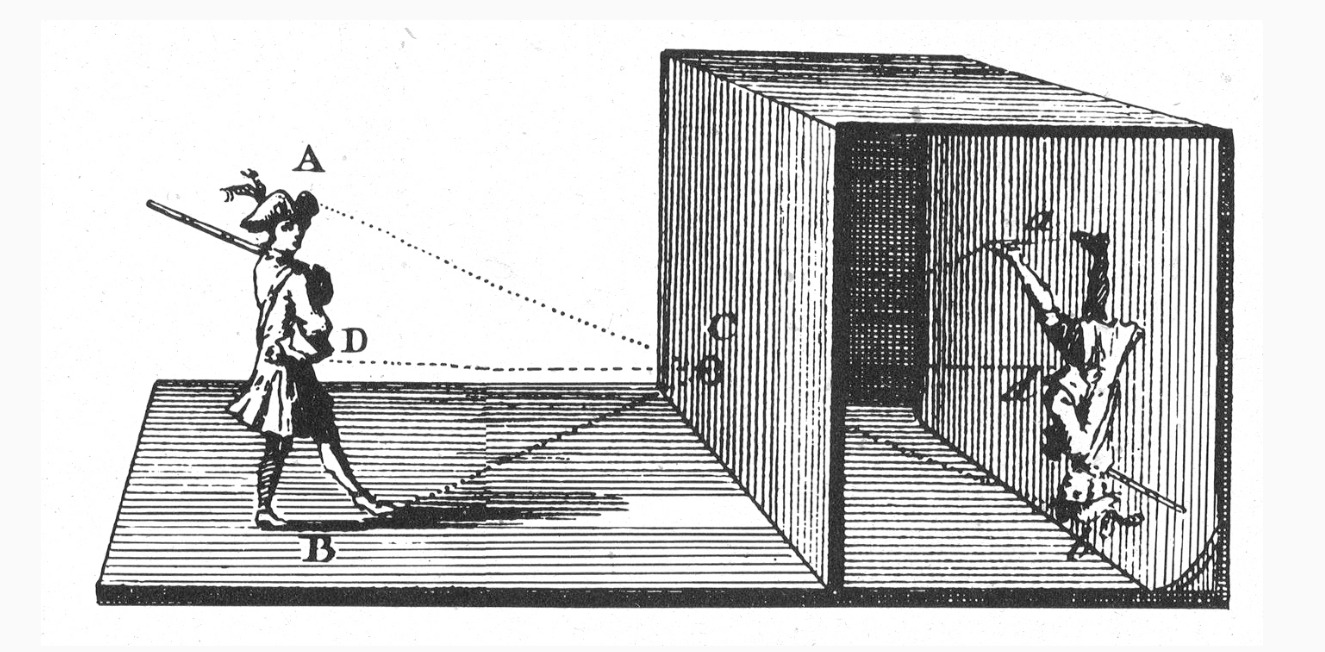
\includegraphics[width=.9\linewidth]{./pics/visio/camera-obscura.jpg}
\end{center}

In such mechanism, only some selected ray lights are allowed inside the
dark room - light rays reach the end of the room and form a \emph{reverted
image} in the wall.

The camera obscura principle was first depcited by \emph{Leonardo da Vinci}
(1452-1519), and after developed by \emph{Johann Zahn} (1641-1707) to build
the first portable camera. Subsequent development led to took the first
photo by \emph{Joseph Nicépore Niépce} in 1826.

Camera obscura can be further summarized in the \emph{pinhole camera} model.

Basically, we need it because it's the only way we have to effectively
collect raylights from a figure, projecting them to a plane that can
capture them.

\subsection{Geometrical description of the pinhole model}
\label{geometrical-description-of-the-pinhole-model}
Pinhole camera principles are the following:

\begin{itemize}
\item put a film in front of a scene;
\item rays departing from the same point of the scene reach the film in
\end{itemize}
different places; conversely, rays departing from different points of
the scene, reach the film in the same place; ideally, a single light
ray from the scene should reach the image plane in a given point; put
in between a barrier with a hole - \textbf{the pinhole}:

\begin{center}
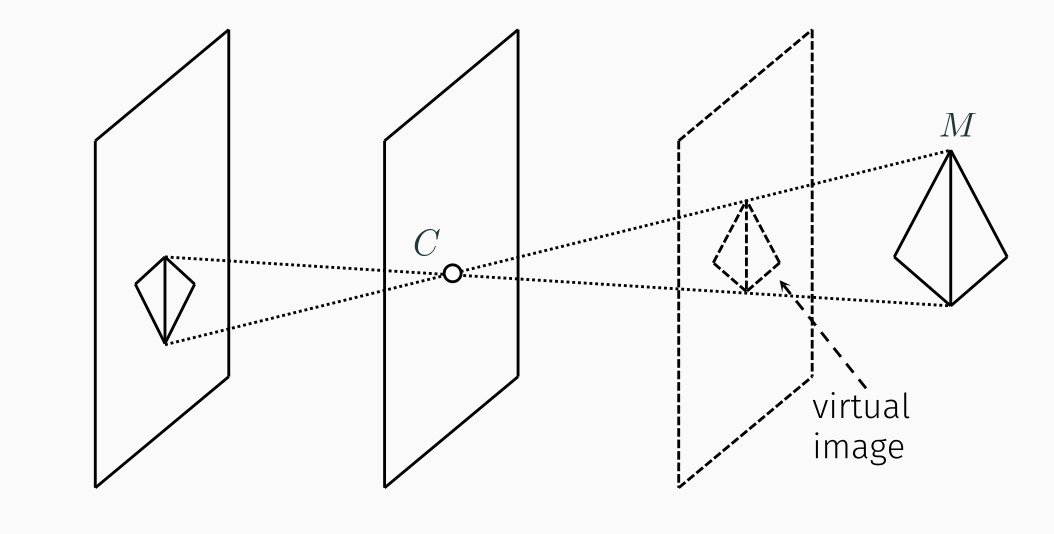
\includegraphics[width=.9\linewidth]{./pics/visio/pinhole1.jpg}
\end{center}

\begin{itemize}
\item The image is then reversed upside-down and left-right
\item A virtual image is formed in front of the camera.
\end{itemize}

\begin{center}
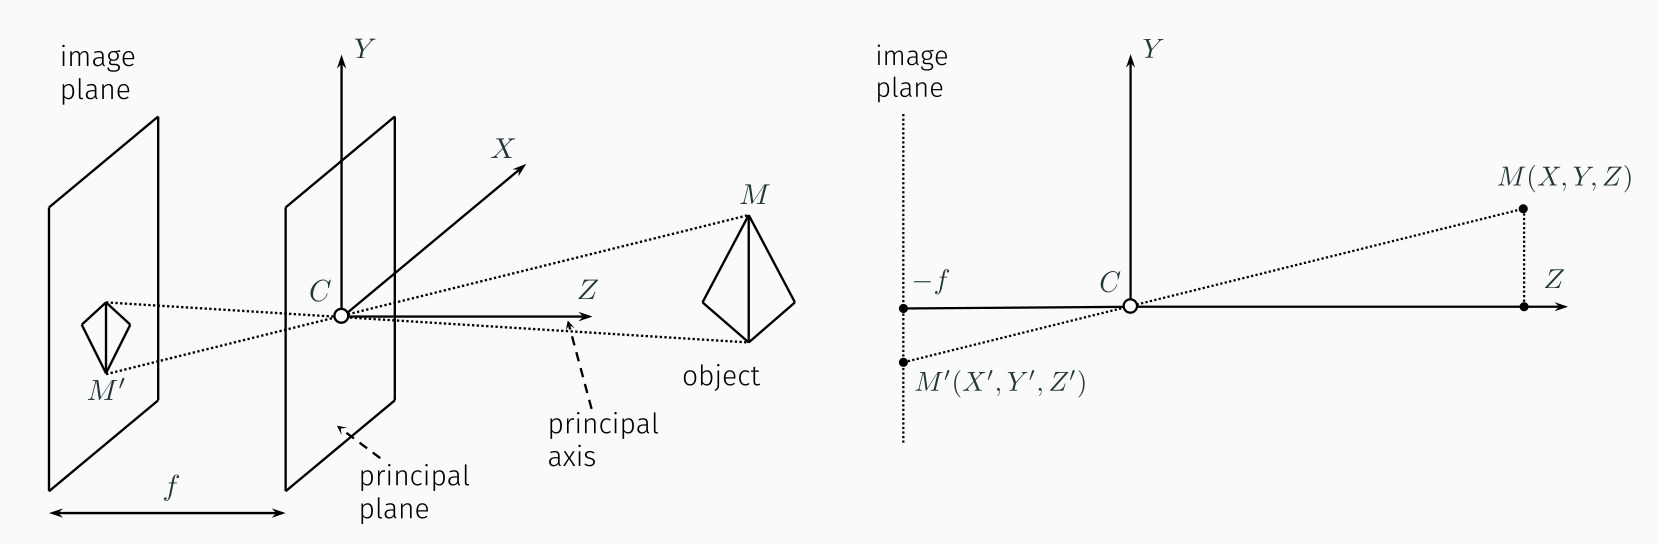
\includegraphics[width=.9\linewidth]{./pics/visio/pinhole2.jpg}
\end{center}

Design of pinhole camera is better described in the Figure, where we
have an object \(M\) at a distance \(Z\) from the pinhole, and the plane
where the pinhole lives is called \emph{principal plane}, from which it is
defined an orthogonal \emph{principal axis} starting from the pinhole spatial
location. Pinhole \(C\) is called \emph{optical center}; it allows some rays
from the object to trepass the principal plane and to reach the \emph{image
plane}, in which we will put a sensor element. Both image and principal
planes are perpendicular together. Distance between such planes is
called \emph{focal length} \(f\).

Following the camera obscura principle, point \(M(X,Y,Z)\) is mapped
into \(M'(X',Y',Z')\) in the image plane. The object appears to be
\emph{reversed}.

\subsection{Perspective}
\label{perspective}
At right, we have a perspective projection of the same scheme. By
similarity of triangles construction, we will have that

\[ [X', Y', Z']^T =  [-\frac{f}{Z}X, -\frac{f}{Z}Y, -f]^T,\]

because of the similarity relationship of \[\frac{M'}{f} = \frac{M}{Z}\]
hence the ratio \[\frac{M'}{M} = \frac{f}{Z} \equiv \varrho.\] The latter is
called \emph{perspective scale factor}, and it describes the effect for which
farther away objects appear smaller. The far the object moves, the
smaller the shrinking due to perspective scale factor is.

Hence,

$$ \begin{bmatrix}X' \\ Y' \\ Z'\end{bmatrix} = \begin{bmatrix} -\varrho X \\ -\varrho Y \\ -\varrho Z\end{bmatrix}$$ and one soon obtains the previous relationship.

In particular, for objects very far from the camera - so that they're
thin (with maximum length \(\Delta Z\)) with respect to their distance
\(Z_0\) from the camera - perspective scale factor \(\varrho\) is roughly constant.
Namely,

\[ \varrho = \frac{f}{Z_0 + \Delta Z} \approx \frac{f}{Z_0} \] due to the
fact that \(Z_0 >> \Delta Z\).

Hence, we can approximate perspective projection such as

\[ X' = -\frac{f}{Z_0}X;\] \[ Y' = -\frac{f}{Z_0}Y.\]

Leonardo da Vinci developed a rule of thumb to understand when the
previous condition holds - that is when \[\frac{\Delta Z}{Z_0} < 0.10,\] or $$Z_0 > 10\Delta z.$$
This rule helps us determine when perspective becomes \emph{weak perspective}
in the sense that it doesn't count much anymore.

\subsection{Aperture and blur}
\label{aperture-and-blur}
Pinhole cameras are - by definition - constructed with \emph{very} small
holes. But, when we leave the mathematics realm and become aware of the
real-world problems, we find out that the pinhole cannot be smaller than
a certain radius.

In particular, too small holes will not allow much light inside, and
thus dark rooms will unsurprisingly be - very dark. What if we increase
pinhole size?

The trouble here is that we are letting more rays inside our dark room -
in particular, \emph{rays from different directions of the same point in the
object will enter the dark room}. Result will be a \textbf{blurred} image,
caused by directions averaging. Instead, if we reduce the pinhole size
too much we will obtain a similar results: when the pinhole size is
comparable to wavelength, diffraction phenomena will start to blur the
image, again.

\begin{center}
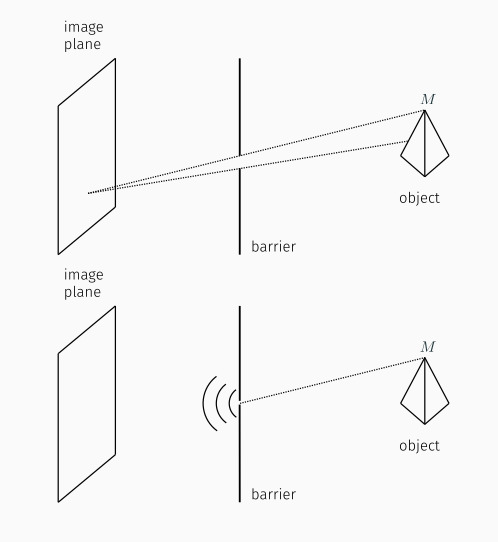
\includegraphics[width=.9\linewidth]{./pics/visio/pinhole3.jpg}
\end{center}

So, a too small pinhole won't allow much light in it (also there will be
some diffraction blurring effects) and a too big pinhole will inevitably
blur the image due to ray directions averaging. Apparently, there's no
solution without pinhole. Many example pictures of both blurring and
diffraction can be found online.

\section{Lenses}
\label{lenses}
Lenses are the solution to the brightness problem. Lenses allow
collection of a larger portion of the ray light, directing it inside the
pinhole. Therefore, a larger amount of light will be let in the dark
room. In particular, we will use the \emph{thin lenses} model, for which
perspective projection criteria still hold true.

A thin lens is composed by a piece of glass (very thin) which has some
particular properties:

\begin{enumerate}
\item rays reaching the centre of the lens will be left untouched;
\item rays coming horizontally will be all directed towards a single point
\end{enumerate}
\(F\), called \emph{focal point};
\begin{enumerate}
\item rays departing from the same point will follow other directions, but
\end{enumerate}
always reach the point \(M^\prime\). That's how more light can actually be collected, as many rays will be collected by the lens and will hit the same point on the image plane.

With these properties we can build our pinhole system with a thin lens.

\subsection{The geometry of a lens system}
\label{the-geometry-of-a-lens-system}
\begin{center}
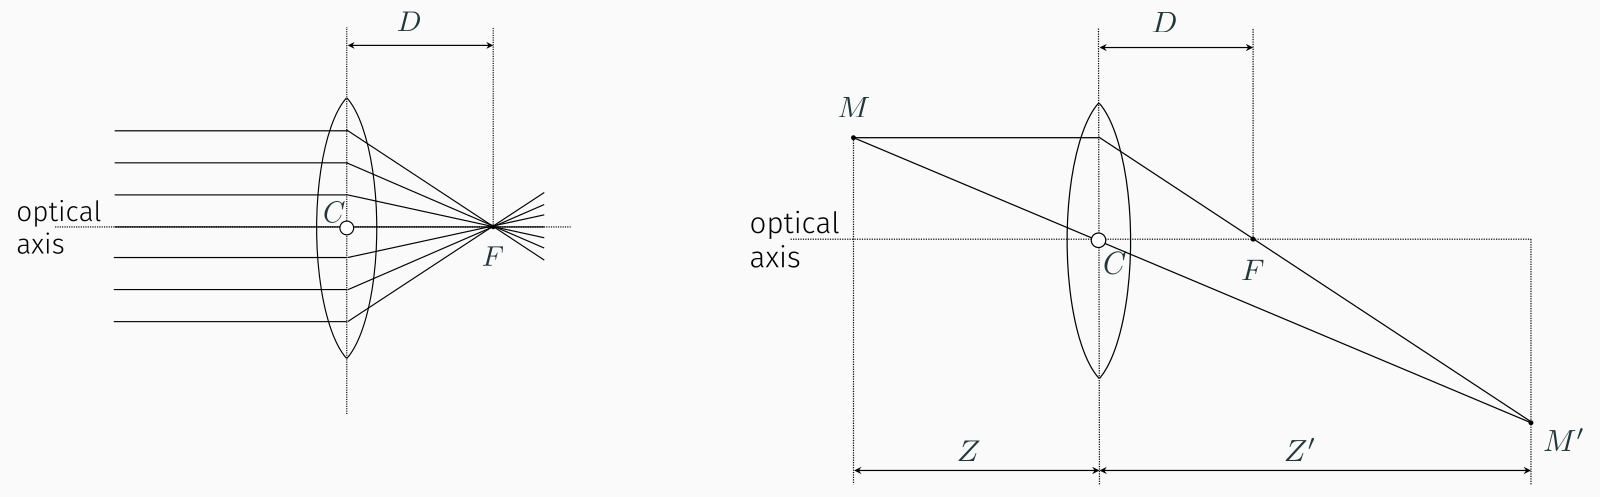
\includegraphics[width=.9\linewidth]{./pics/visio/thin-lens.jpg}
\end{center}

Image above describes the thin lens in detail. Aside from the previously
described focal point \(F\), we define \(D\) \emph{focal length} the distance
between the center \(C\) of the lens and the focal point \(F\), and
\(Z\), \(Z'\) that are, respectively, distances between the lens and the
real object and between the lens and the image plane. An axis orthogonal
to the lens departs from \(C\) - the \emph{optical axis}.

The point \(M'\) on the image plane is reached by two, distinct, rays;
the first one being the one crossing the centre \(C\) of the lens (which
won't change direction due to thin lens properties) and the second one
crossing the focal point \(F\), since each horizontally incident ray
will be directed towards \(F\). The image \(M'\) can be obtained by
intersecting \(2\) rays.

Point \(M\) is projected, when in focus, into the same position of a
pinhole model having its center \(C\) located in the focal point \(F\).
That is, we can get the same results with more rays entering the dark
room (hence, our image will be bright enough to be captured). In fact,
there's a straight line from point \(M\) to point \(M'\), \emph{plus} there
are many rays from such point of the object, collected by the lens and
reaching focal point.

\subsection{The thin lens equation}
\label{the-thin-lens-equation}
By triangles similarities, we can find the following relationships,

\[ \frac{Y'}{Y} = \frac{Z'}{Z} \] and
\[ \frac{Y'}{Y} = \frac{Z' - D}{D}, \]

where we had a look at the two similar triangles at the right of the
lens. Merging the previous equations, we obtain the \emph{thin lens equation}
\[ \frac{1}{Z} + \frac{1}{Z'} = \frac{1}{D}, \] a remarkable formula
which puts \(Z\), \(Z'\) and \(D\) in relationship.

\subsection{Focusing}
\label{focusing}
Thin lens equation explains the \emph{focusing} of a lens with respect to the
distances between the lens and the object or the image plane.

In particular, given distances \(Z\) and \(Z'\), focal length \(D\) will
be determined by the left member of the equation.

\begin{itemize}
\item when \(Z \longrightarrow \infty\) we are focusing the infinite. This
means that the term with \(Z\) vanishes, and the thin lens equation
yields \[ \frac{1}{Z'} = \frac{1}{D},\] and ultimately \(Z'=D\);
\item when \(Z\) = \(Z'\), the only possible solution is \(Z = Z' = 2D\). In
such situation the focal point will be in the middle between the
distance between lens and objects. Since objects distance with respect
to the lens is the same, this is called \emph{1:1 imaging};
\item when \(2D < Z < \infty\), equation implies \(D < Z' < 2D\);
\item when \(D < Z < 2D\), equation yields the viceversa \(2D < Z' < \infty\);
\item when \(Z = D\) focus is impossible, for rays are spread horizontally towards the image plane.
\end{itemize}

Basically, we can't focus objects closer than \(2D\), otherwise our
sensor would have to go back - possibly very much - to keep focus.

\subsection{Field of view}
\label{field-of-view}
We can define the \emph{field of view} of a camera system as the portion of
the scene space that projects onto the sensor.

Field of view \(f.o.v = 2\varphi\) depends largely on the focusing
distance and the sensor width \(w\), and it is conventionally defined by
focusing at infinity; for instance,

\[ f.o.v. \equiv 2\varphi = 2\arctan{\frac{w}{2D}}.\]

Field of view can be understood as the maximum angle \(2\varphi\) for
which a ray crossing the lens could reach any portion of the sensor of
width \(w\).

\begin{center}
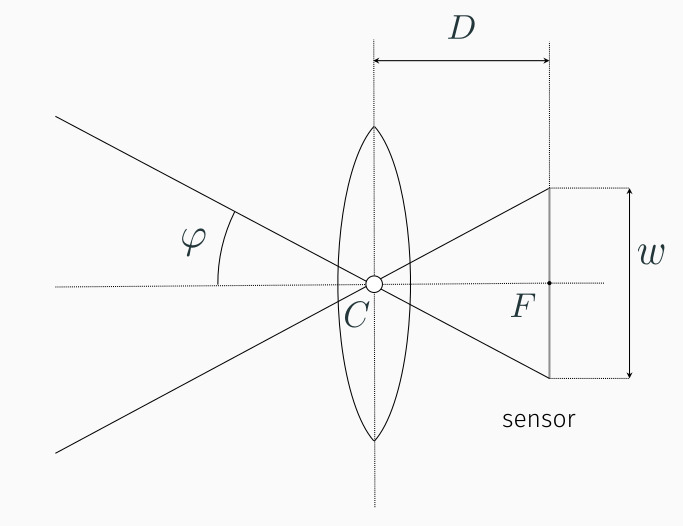
\includegraphics[width=.9\linewidth]{./pics/visio/field-of-view.jpg}
\end{center}

\subsection{The circle of confusion (blur circle)}
\label{the-circle-of-confusion-blur-circle}
Image is perfectly on focus when all rays from point \(M\) are projected
into \(M'\). Such condition holds when the image plane is congruent with
the \emph{focus plane}.

A phenomena happening when the image plane is not on the focus plane,
but at a distance \(\Delta Z'\) from it, is the so-called \emph{blurring
circle}, also called \emph{circle of confusion}. The blurring circle is
caused by the misalignment of the image plane from the focus plane: rays
projected from point \(M\) of the object will reach the image plane in
different locations instead of a single point \(M'\). This causes a
blurring of the image in the circle where the rays are incident.

\begin{center}
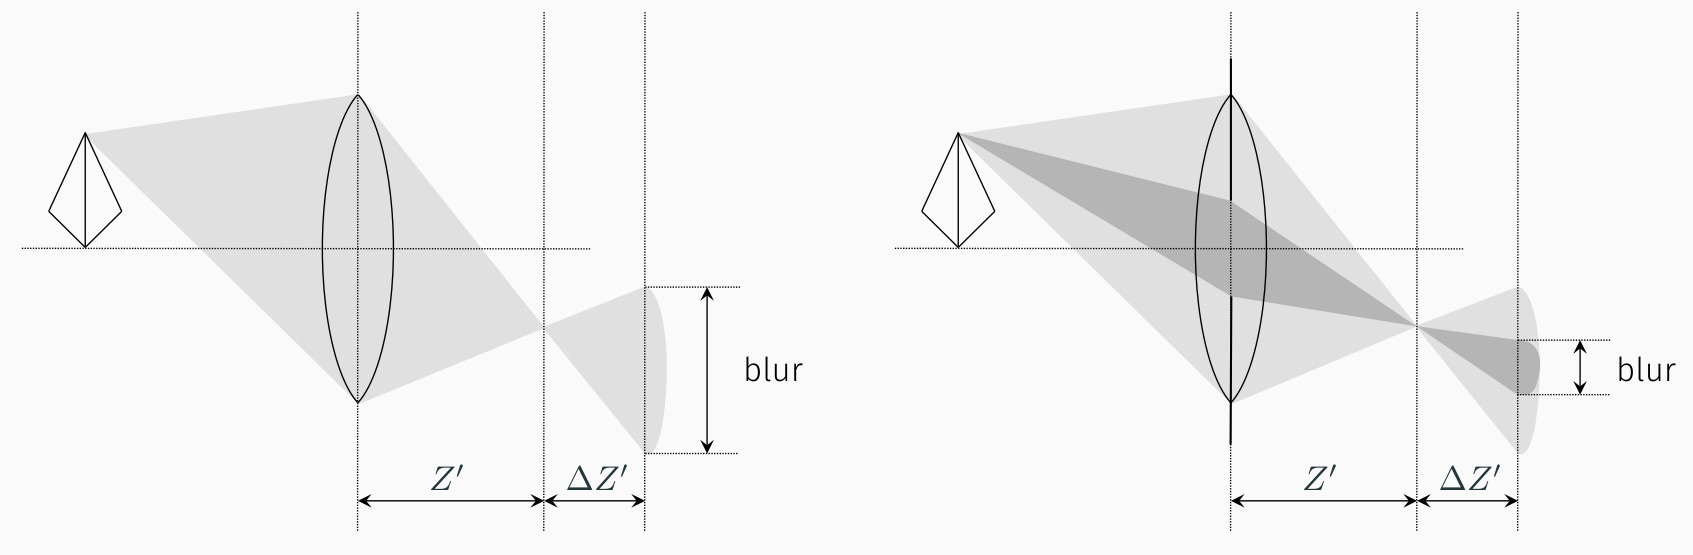
\includegraphics[width=.9\linewidth]{./pics/visio/blur-circles.jpg}
\end{center}

A blur circle diameter is given by the formula

\[d_{blur} = d\cdot\frac{|\Delta Z'|}{Z'},\]

where \(d\) is the lens diameter and the expression is obtained using
triangles similarities. In fact, we have
\[ \frac{d_{blur}}{d} = \frac{\Delta Z'}{Z'}.\]

Blurring prevents getting sharp and detailed images: therefore, we must
avoid getting blur effects on our images.

To partially solve our problem, we could reduce the aperture, since
reducing the diameter of the lens will cause less rays to enter the dark
room and eventually less of them will reach the sensor, resulting in a
minor blurring effect.

This is shown in figure above, where the right picture visually explains
such solution, and this can be assumed to be true since reducing \(d\)
in the formula directly causes a decreasing of the term \(d_{blur}\).

This phenomena is far more complex than the above explanation. For
instance, suppose we have a moving image plane which will change its
location according to the distance of the object to keep in focus. If we
keep a huge aperture, we are basically making more room for blurring
effects of objects out of focus. This will result in a proper focusing
of an object, while quickly blurring objects with a different distance
from the camera with respect to the object. Instead, if we take a
smaller aperture, our lens will allow less blurring of objects out of
focus. This means that objects out of focus will not exhibit blurring
even if they're at a different distance from the camera. Sadly, closing
the lens will complicate image acquiring, since the lens would let less
light in the dark room.

In the end, it all depends on the kind of effect we want to obtain, and
the exposure of the object, since aperture is a trade-off between
focusing capabilities and brightness of the object whose image is
captured.

\begin{center}
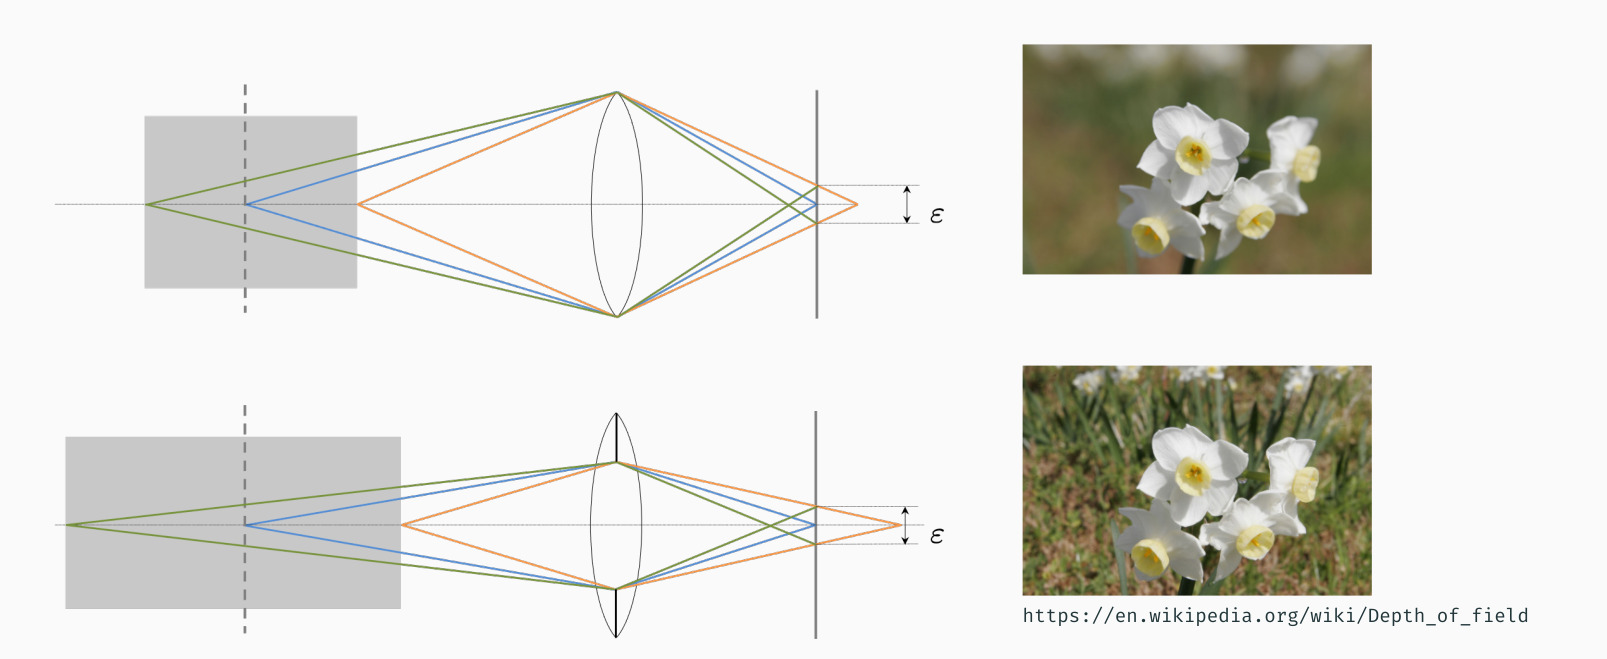
\includegraphics[width=.9\linewidth]{./pics/visio/focusing-blur.jpg}
\end{center}

\subsection{Telecentric optics}
\label{telecentric-optics}
A particular kind of optics is the \emph{telecentric optics}. Telecentric
cameras are special ones that capture an orthogonal projection of the
image.

To achieve that, we put a pinhole exactly in the focal point \(F\). By
doing so, our camera will capture only rays which are travelling
parallel to the lens axis, so that objects at different distances will
appear at the same distance in space.

\begin{center}
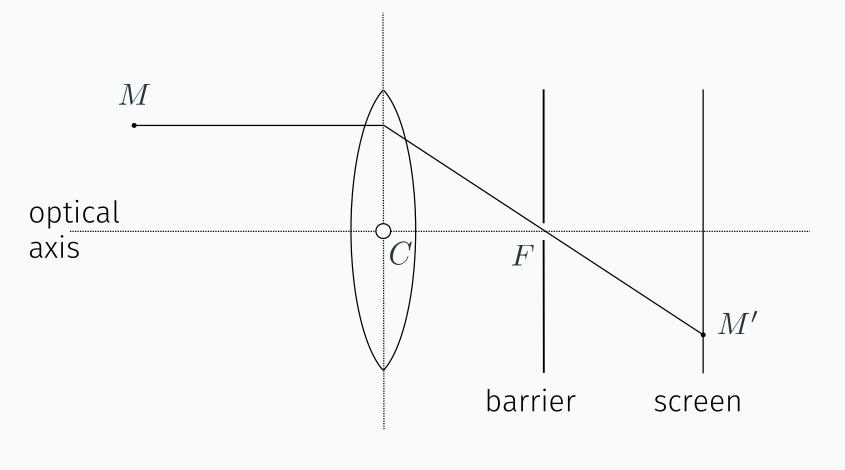
\includegraphics[width=.9\linewidth]{./pics/visio/telecentric-optics.jpg}
\end{center}

\subsection{Thick lenses}
\label{thick-lenses}
When we abandon the thin lens hypothesis, we get the so called \emph{thick
lens}. Thick lenses have different portions of the lens with different
focal points. Distortion acts \emph{radially}, so we can mathematically
compensate it. Thick lenses suffer from side effects such as \emph{radial
distorsion} (straight lines become curve), \emph{pincushion distorsion}
(increasing magnification) and \emph{barrel distorsion} (decreasing
magnification).

\begin{center}
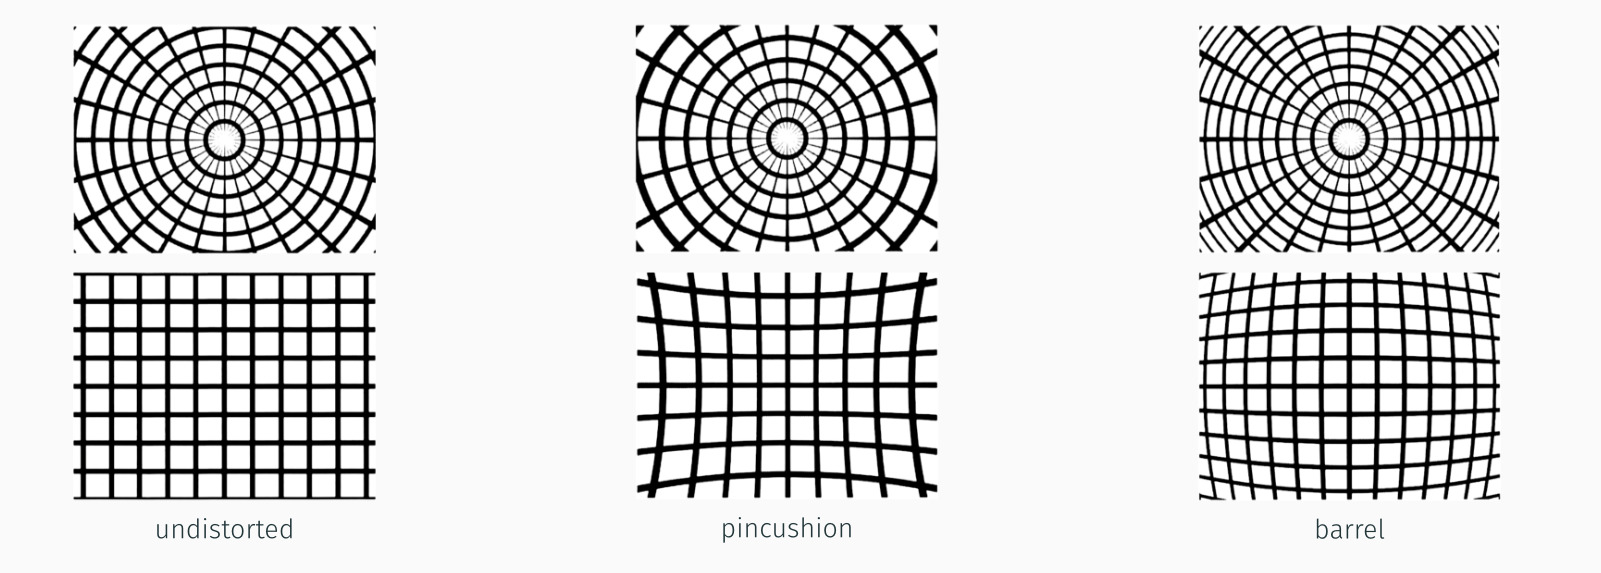
\includegraphics[width=.9\linewidth]{./pics/visio/distortion.jpg}
\end{center}

\begin{center}
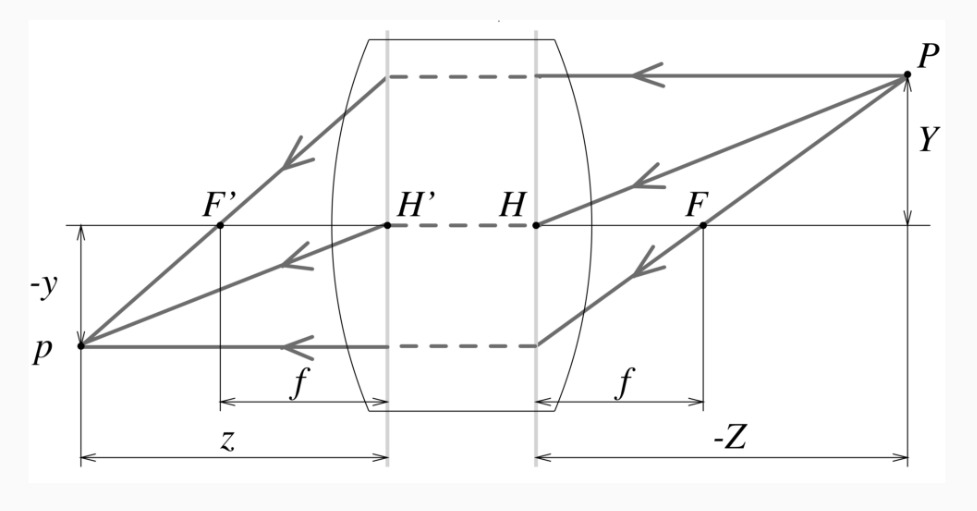
\includegraphics[width=.9\linewidth]{./pics/visio/thick-lens.jpg}
\end{center}

Real lenses also suffer from a lot of other side effects, such as
\emph{vignetting}, \emph{chromatic aberration} and so on.

Different wavelengths travel with different paths in the lens, resulting
in a wave decomposition by color - this phenomena will appear in a
similar fashion of a blur, with color artifacts.

\begin{center}
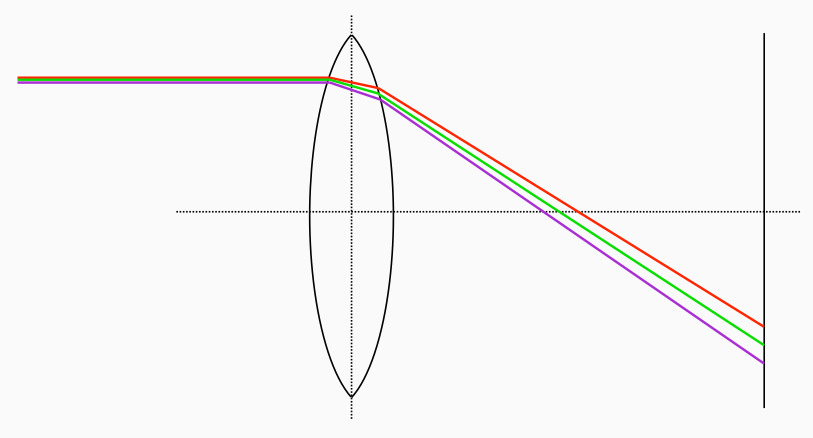
\includegraphics[width=.9\linewidth]{./pics/visio/chromatic-aberration.jpg}
\end{center}

To solve this, a second \emph{compound lens} can be added. However, adding a
second lens will result in a further side effect, such as \emph{vignetting}.
Vignetting happens when a portion of the light doesn't reach the second
lens, resulting in the outer portion of the image to be darker.

\begin{center}
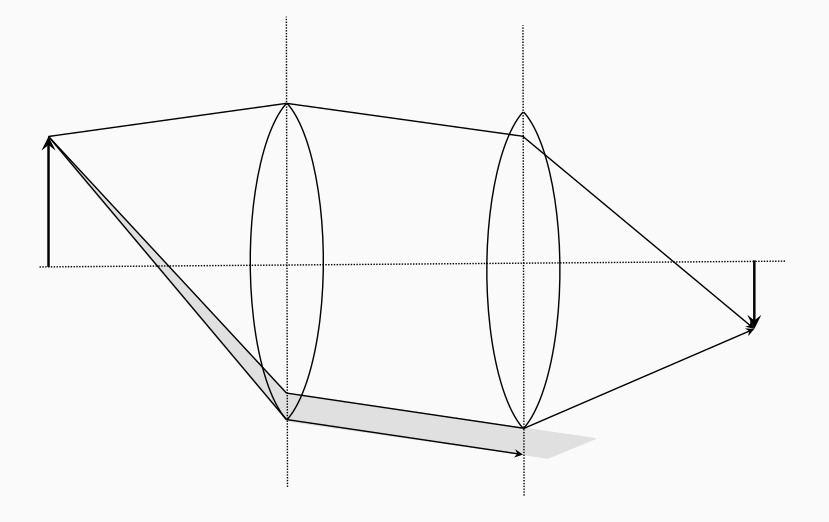
\includegraphics[width=.9\linewidth]{./pics/visio/vignetting.jpg}
\end{center}

\section{Ray capturing}
\label{ray-capturing}
\subsection{Sensing}
\label{sensing}
Sensing happens through \emph{pixels}. Ray lights reach the lens first, and
then photosensitive elements can capture them. A single sensor apparatus
is called a pixel. When light reaches a photosensitive element, an
electric current is generated proportional to the amount of light
received. More light a sensor receives, the more current will flow in
the circuit. Current charges a capacitor, which is periodically
discharged to measure the amount of charge in it. Such period of time is
called \emph{shutter time}, and corresponds to the framerate of the camera.

We capture color through the \emph{three sensors method}. There's a sensor
sensitive to each channel: red, green and blue. A set of glass prisons
will split wave to 3 different colors, sending them to the three
different sensors. Location of sensors is determined by the \emph{Bayer
Mosaic}, as in the figure.

\begin{center}
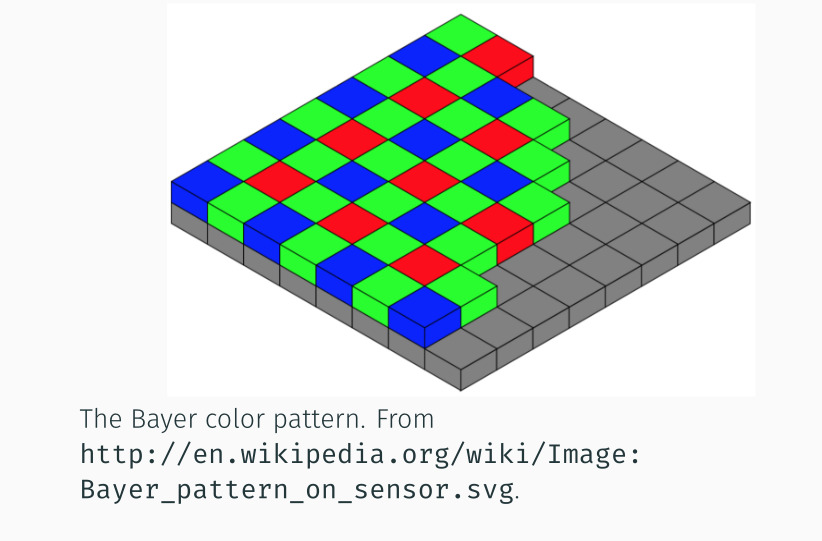
\includegraphics[width=.9\linewidth]{./pics/visio/bayer-mosaic.jpg}
\end{center}

In the square of pixels, green is \emph{overrepresented}: this is okay with
the fact that human eyes see much better the green color than red or
blue.

\subsection{The diagram of light capturing}
\label{the-diagram-of-light-capturing}
A simple sensor model is composed by

\begin{itemize}
\item an \emph{integrator}, for instance a capacitance element;
\item a \emph{sampler}, used to sample the amount of charge from the capacitor;
\item a \emph{quantizer}, necessary to convert such information to a number.
\end{itemize}

Noise will enter this process. In particular, we have noise entering the
capacitor, and entering the quantizer. Noise will largely depend on
input brightness, camera settings and camera gain.

\begin{center}
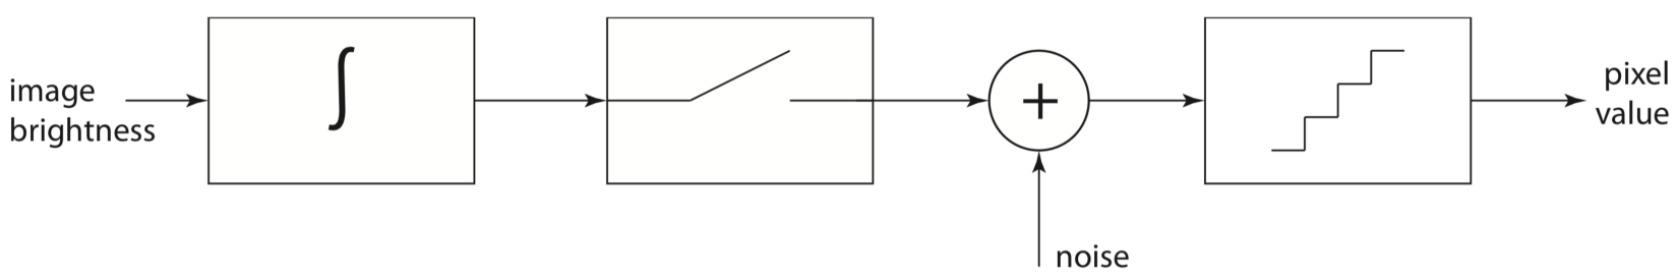
\includegraphics[width=.9\linewidth]{./pics/visio/light-capturing.jpg}
\end{center}

\part{Early Vision}
\label{sec:orgd85bc00}
\chapter{Basics of Image Processing}
\label{basics-of-image-processing}
\section{Linear filters}
\label{linear-filters}
\subsection{The description of an image}
\label{the-description-of-an-image}
An image can be described by the function
\[f: \mathbb{R}^2 \longrightarrow \mathbb{R},\] where \(f(x, y)\) yields
\emph{intensity} of a feature (brightness) at location \((x, y)\). The domain
is usually a rectangle, and intensity is bounded, so the function will
be defined as \[f:[a, b] \times [c, d] \longrightarrow [I^-, I^+].\]

We can split intensity in color intensity with a vector function. For
instance, each element of the vector will contain intensity of,
respectively, red, green and blue:

\[f(x, y) = \begin{bmatrix} r(x, y)\\ g(x, y)\\ b(x, y) \end{bmatrix}, \]

each one with its own upper and lower bound. Color intensities are named
\emph{channels}. Overall intensity is obtained with a linear combination of
red, green and blue channels with experimentally obtained coefficients.

Digital images are obtained by first \emph{sampling} the 2D space on a
regular grid, and then \emph{quantizing} the value:

\[ f(i, j) = \mbox{ Quantize }(f(\Delta i, \Delta j)).\]

An image can thus be represented as a matrix with indexes \(i\) and
\(j\): each channel is actually a matrix of values, that are the results
of previous samples and quantization. The higher the value in the matrix
field, the greater the intensity will be for that specific pixel.

Each channel is typically represented as a \(8\) bits value, ranging
from \(0\) to \(255\).

\subsection{Linear filters}
\label{linear-filters-1}
A \emph{operator} is a function \(h(\cdot)\) that takes an image as input and
outputs another image \(g\) such as

\[ g(i, j) = (h \circ f) = h(f(i, j)).\]

An operator is said to be \emph{local} if a given value of a pixel depends on
a collection of pixel values in the neighborhood. For instance, a local
operator could be one that makes the average of a pixel value with all
its surrounding neighbors. Such operator would work on a \emph{window} of
\(2W + 1\) pixels.

\subsection{The averaging filter}
\label{the-averaging-filter}
An \emph{averaging} filter can be mathematically defined as

\[ g(i, j) = \frac{1}{(2W + 1)^2} \sum_{k = -W}^{k=W} \sum_{l = -W}^{k=W} f(i + k, j + l).\]
If \(W=1\), the above formula will perform the average of all pixels
with its directly surrounding neighbors, for instance:

\[ g(i, j) = \frac{1}{9} \sum_{k = -1}^{k=1} \sum_{l = -1}^{k=1} f(i + k, j + l).\]

The average local operator in a \(3 \times 3\) square can be understood
as the sum of all 9 cells values, with each one with a weight of
\(1/9\). By putting \(W=1\) we obtained a \(3 \times 3\) square, a
\emph{mask} of pixels. Such mask determined by the operator is called
\emph{kernel} of the filter.

In above example, we had a kernel filter with size \(3 \times 3\), and
with \(\frac{1}{9}\) as value for all its cells. Much more complex
filters can be achieved, for instance we can define a generic \emph{weighted
sum} filter as

\[ g(i, j) = \sum_{k = -W}^{k = W} \sum_{l = -W}^{l = W} f(i + k, j + l) h(k, l)\]

with \(h\) kernel of the filter having possibly different values for
each location \((k, l)\) of the mask.

\subsection{Correlation filter}
\label{correlation-filter}
A special local filter is the \emph{Correlation} filter:

\[ g(i, j) = f \otimes h (i, j) = \sum_{k, l} f(i + k, j + l) h(k, l)\]

Correlation can be described as an averaging filter, but with a mask
having different coefficients instead of fixes ones. It is basically the
weighted sum filter we briefly discussed above.

\subsection{Convolution filter}
\label{convolution-filter}
A remarkable filter is the \emph{Convolution} filter,

\[ g(i, j) = f * h = \sum_{k, l} f(i - k, j - l) h(k, l) = \sum_{k, l} f(k, l) h(i - k, j - l).\]
Convolution works in a different fashion than correlation, in particular
convolution performs weighted sum of pixels which are \emph{at the opposite
location of the corresponding kernel filter location}. For instance,
suppose we have a \(3 \times 3\) mask, enumerating all pixels from top
to bottom, left to right, \(1\) to \(9\). We will perform a convolution
with pixel at location \(5\) as center. Pixels in image that are at
location \(1\) and \(2\), will be, respectively, filtered with values of
the kernel that are in the opposite location, \(9\) and \(8\).

Properties of convolution and correlation together are the following:

\begin{itemize}
\item they are \emph{shift-invariant}: the output depends on pattern of
neighborhood pixels rather than position of currnet neighborhood
\[g(i, j) = f(i + k, j + l) \Leftrightarrow (h \circ g)(i, j) = (h \circ f)(i + k, j + l);\] -
they are \emph{linear}: for them holds the superposition principle
\[h \circ (\alpha f + \beta g) = \alpha(h \circ f) + \beta(h \circ g), \mbox { with } \alpha, \beta \in \mathbb{R}.\]
Properties of convolution alone are the following:

\item is \emph{commutative};

\item is \emph{associative};

\item its fourier transform has the remarkable property
that \[ f * g \longleftrightarrow F\cdot G,\] with the
\(\longleftrightarrow\) symbol denoting a fourier transform (and
viceversa) of an entire equation. This is very important: \textbf{a
convolution can be computed as a simple product in the Fourier
transform space}, thus allowing for far quicker calculations.
\end{itemize}

\subsection{Kernel of a filter}
\label{kernel-of-a-filter}
The \emph{kernel} is the \emph{mask} of the filter, a fixed-size matrix which will
correspond to the local filter window employed when filtering.

Since convolving a function \(h\) with the \emph{Dirac's delta impulse}
\(\delta\) yields the same function again \(\delta * h = h\), we will
say that the kernel of the convolution is the \emph{impulse response
function}, or \emph{unity impulse}.

\subsection{Border effects}
\label{border-effects}
A problem with such filter happens when we are averaging the border
pixels. Such pixels will need to be treated differently, for instance we
could ignore them, remove them, or simply perform the average with a
different algorithm and ignoring some out-of-the-image locations.

A common operation is to use a \emph{padding} technique to extend the
original image. To do so, we will set aside pixels with constant value
(this is called \emph{clamping}), or repeating the same value in the border.
More complex solutions involve wrapping the image as a toroid or a
sphere, or mirroring the pattern by reflecting pixels.

These operations are shown in the Figure.

\begin{center}
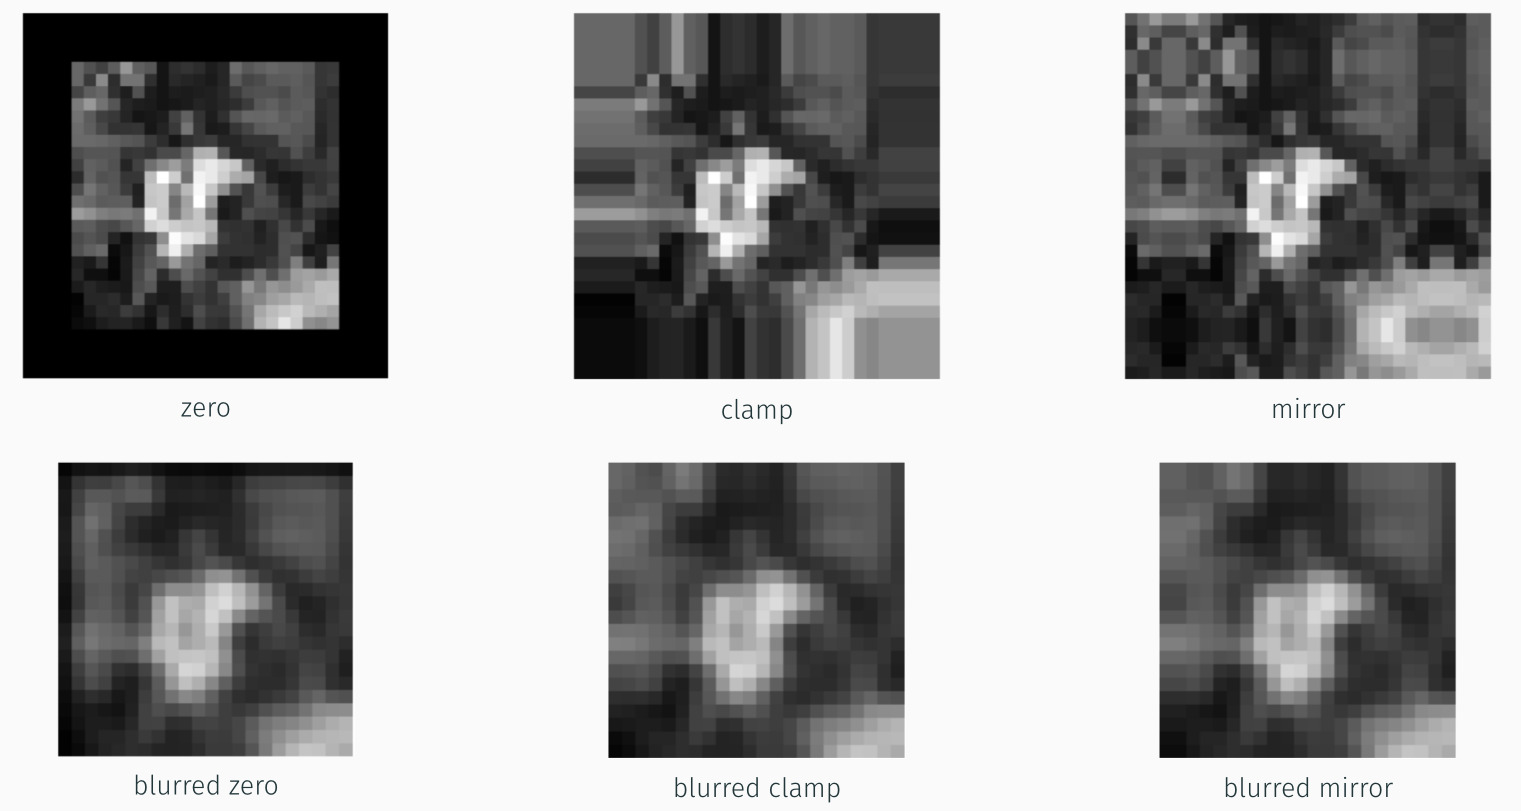
\includegraphics[width=.9\linewidth]{./pics/proc/border-effects.jpg}
\end{center}

\subsection{Remarkable linear filters}
\label{remarkable-linear-filters}
Some remarkable linear filters are the \emph{box filter}, the \emph{Gaussian
filter}, the \emph{bilinear filter}, the \emph{Sobel filter} and the \emph{corner
filter}. Box, Gaussian and bilinear filter are \emph{low-pass} filters, while
Sobel and corner filter are \emph{band-pass} filters. Low-pass filters will
remove much of the high-frequency content of the images, while band-pass
will remove both very-low and very-high frequency content. All filters
are \emph{not oriented}; the Sobel filter only is said to be \emph{oriented}.

The box filter averages the pixel values in a square window. Its shape
is of the form

\[ h = \frac{1}{9} \begin{bmatrix} 1 & 1 & 1 \\ 1 & 1 & 1 \\ 1 & 1 & 1 \end{bmatrix}. \]

Basically, each element would have a value of \(\frac{1}{9}\), and the
end result will be the average of the pixels around the filtered one.

The Gaussian filter does the same, but in a better fashion. For
instance,

\[ G(x, y; \sigma) = \frac{1}{2 \pi \sigma^2} \exp{\left(-\frac{x^2 + y^2}{2\sigma^2}\right)}.\]

Such formula is the formula of a gaussian with \emph{variance} \(\sigma^2\)
(\(\sigma\) is its standard deviation).

The quantity \(\sigma\) is associated to the \emph{width} of the filter, for
it controls the size of the neighborhood that actually affects the
center pixel when evaluating the filter and producing the filtered
image. Even though there's a fixed window, the exponential would still
be close to zero after a certain distance, that depends on the
\(\sigma\): the smaller it is, the smaller that distance will be. As a
result, smaller \(\sigma\)s will basically leave the image unaffected,
as the Gaussian filter with \(\sigma\) going to \(0\) will resemble more
and more the impulse filter (which, as we know, is the kernel of the
convolution, so that doing such filtering would leave the image
unaffected \(f * \delta = f\)). On contrary, increasing \(\sigma\) value
will yield images which will see their details lost. This particular
effect is due to the low-pass filtering nature of the Gaussian filter,
which is suited to remove details in the image.

A kernel for the Gaussian can be obtained by constructing a proper
\((2W + 1)^2\) array, such that

\[h(i,j) = \frac{1}{2\pi \sigma^2} \exp{\left(-\frac{(i - W - 1)^2 + (j - W - 1)^2}{2\sigma^2}\right)}.\]

\begin{center}
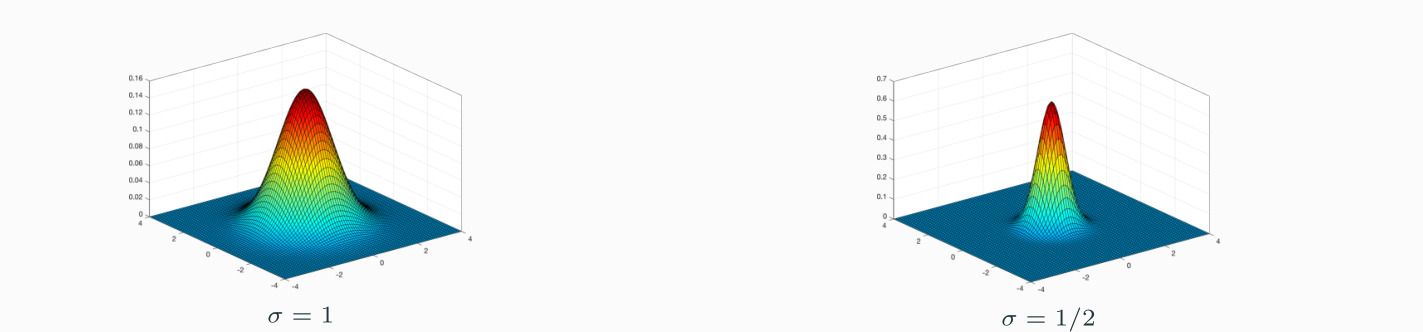
\includegraphics[width=.9\linewidth]{./pics/proc/gaussian-sigma.jpg}
\end{center}

The bilinear filter has a kernel that is the product of two, piecewise
linear, \emph{tent} functions,

\[\frac{1}{16} \begin{bmatrix} 1 & 2 & 1\\ 2 & 4 & 2\\ 1 & 2 & 1 \end{bmatrix} = \frac{1}{4}\begin{bmatrix} 1 \\ 2 \\ 1 \end{bmatrix} \frac{1}{4} \begin{bmatrix} 1 & 2 & 1 \end{bmatrix} \]

The Sobel filter, which instead is an oriented band-pass filter, has a
different shape,

\[ \frac{1}{8} \begin{bmatrix} -1 & 0 & 1 \\ -2 & 0 & 2 \\ -1 & 0 & 1 \end{bmatrix} = \frac{1}{4} \begin{bmatrix} 1 \\ 2 \\ 1 \end{bmatrix} \frac{1}{2} \begin{bmatrix} -1 & 0 & 1 \end{bmatrix} \]

The last filter, the corner filter, is a non-oriented band-pass filter,

\[ \frac{1}{4} \begin{bmatrix} 1 & -2 & 1\\ -2 & 4 & -2\\ 1 & -2 & 1\\ \end{bmatrix} = \frac{1}{2} \begin{bmatrix} 1 \\ -2 \\ 1 \end{bmatrix} \frac{1}{2} \begin{bmatrix} 1 & -2 & 1 \end{bmatrix}. \]

\section{Band-pass filters}
\label{band-pass-filters}
Band-pass filters are any filter that passes frequencies in a certain
range, and attenuates frequencies that are outside that range.

\subsection{Laplacian of Gaussian}
\label{laplacian-of-gaussian}
A more sophisticated filter can be created by means of two passages,

\begin{enumerate}
\item we first smooth the image with a Gaussian filter in order to remove
high frequency content;
\item we take the first or the second derivative of that image.
\end{enumerate}

The trick here is that we \emph{take both steps by convolving the image with
a single function}, the \textbf{Laplacian of Gaussian}. Let's start with the
\emph{Laplacian}. Laplacian of a function is the quantity

\[\nabla^2 f(x, y) = \frac{\partial^2 f}{\partial x^2} + \frac{\partial^2 f}{\partial y^2},\]
and corresponds to a ``second derivative'' of a function \(f\) of two
variables (our image).

Basically, the idea of a LoG filter is to simply convolve \(f\) with the
Laplacian of the Gaussian filter, which is the quantity

\[\nabla^2 G(x, y; \sigma) = \left(\frac{x^2 + y^2}{\sigma^4} - \frac{2}{\sigma^2}\right) G(x, y; \sigma),\]

which is the Gaussian function multiplied by a function which depends on
both \(x^2\) and \(y^2\).

\begin{center}
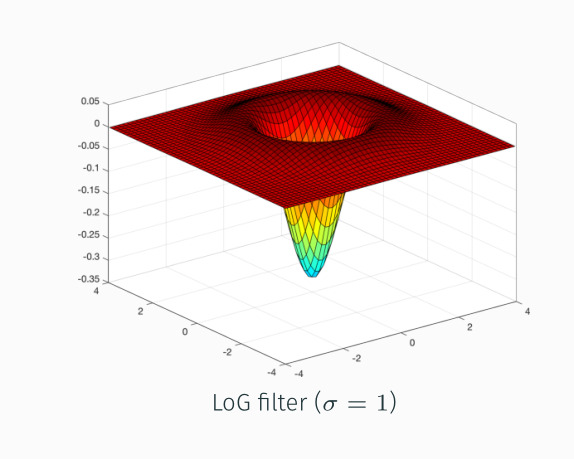
\includegraphics[width=.9\linewidth]{./pics/proc/log-filter.jpg}
\end{center}

As one can see in the figure, LoG filter is \emph{not oriented} and has a
\emph{center-surround} response.

\subsection{Derivative of Gaussian}
\label{derivative-of-gaussian}
DoG stands for \textbf{Derivative of Gaussian}, and is a different kind of
filter which is very similar to the LoG. The idea here is to just take
the \emph{gradient} (the directional derivative) of the Gaussian. In
particular, let's take
\(\nabla f = (\frac{\partial f}{\partial x}, \frac{\partial f}{\partial y})\)
the gradient of \(f\): its \emph{directional derivative} along a direction
\(d = (u, v) = (\cos\theta, \sin\theta)\) is the dot product between a
vector \(d\) and the gradient of \(f\), that is

\[\nabla_d f = d \cdot \nabla f.\] Such quantity is of a crucial
importance. Suppose that we want to compute a band-pass filter,
employing first-order directional derivatives. One has to do

\[\nabla_d (G * f) = (\nabla_d G) * f = (d \cdot \nabla G) * f,\] but
the quantity
\[d \cdot \nabla G = u\frac{\partial G}{\partial x} + v\frac{\partial G}{\partial y}.\]
Resulting filter is called \textbf{steerable filter}, due to the fact that it
can be fine-tuned by choosing the value of \(u = \cos\theta\) and
\(v=\sin\theta\), directions in the image plane, accordingly to our
needs. Basically, this kind of filter has a \emph{direction} which can be set
up by taking proper values of \(u\) and \(v\): we can assign a direction
to such filter, thus we call it \emph{steerable}.

\subsection{Steerable filters}
\label{steerable-filters}
We have the quantity
\[d \cdot \nabla G = u\frac{\partial G}{\partial x} + v\frac{\partial G}{\partial y}.\]
Such filter is called \textbf{steerable filter}, due to the fact that it can be
fine-tuned by choosing the value of \(u = \cos\theta\) and
\(v=\sin\theta\), directions in the image plane, accordingly to our
needs. Basically, this kind of filter has a \emph{direction} which can be set
up by taking proper values of \(u\) and \(v\): we can assign a direction
to such filter, thus we call it \emph{steerable}.

Steerable filters are crucial for efficiency: the core idea is that we
can compute the basis filter (the Gaussian) \emph{once}, and then simply take
the dot product with the direction \(d\) we want to set to the filter.

A basis filter is the filter having the default direction (direction is
along axis). In formula,

\[d \cdot \nabla G = u\frac{\partial G}{\partial x} + v\frac{\partial G}{\partial y} = u G_x + v G_y,\]
basis filters are \(G_x\) and \(G_y\). It is sufficient to compute each
one of them once by convoluting \(f\) with the basis filters, and then
apply the dot product to get a new filter of the same shape along the
direction \(d\) we imposed.

\subsection{The idea of basis filters}
\label{the-idea-of-basis-filters}
DoG only requires two filters, as shown above. Such filters are those
over direction \(x\) and \(y\). Computing the gradient of the Gaussian
and then convolving it with the image is, then, sufficient.

LoG requires at least three basis filters. In particular, given the
second order derivative of the Gaussian, with respect to \(x\),

\[G_{xx} = (4x^2 - 2)\exp{\left(-\frac{x^2 + y^2}{2\sigma^2}\right)},\]
having \(u_i = (\cos\theta_i, \sin\theta_i)\), it has been proposed that
\[G_{uu} = \sum_{i=1}^3 k_i(\theta)G_{u_i, u_i},\]

where \(G_{u_i, u_i}\) is the second derivative of Gaussian with respect
to a direction \(u_i\), \(k_i\) is a term such that
\[k_i(\theta) = \frac{1}{3}[1 + 2\cos(2(\theta - \theta_i))],\] and the
angle \(\theta_i\) has values \(\theta_1 = 0\),
\(\theta_2 = \frac{\pi}{3}\) and \(\theta_3 = \frac{2\pi}{3}\).

Basically, one has to just compute \(G_{u_i, u_i}\), and to compute the
generic filter in direction \(u\) one makes the sum with three terms
multiplied by \(k_i(\theta)\), where \(\theta\) is the angle upon which
the direction \(u\) depends.

\subsection{High pass filtering}
\label{sec:org8e6ba18}
A high-pass filter can be built by \emph{subtracting} a low-pass filtering
result from the image (basically, by ``removing'' low frequencies by
subtraction). Adding such high-pass filtered result to the image by a
fraction of its value, can yield a sharper image whose details are
augmented.

Basically, a sharper image can be obtained in such way,

\[f_{sharp} = f + \gamma(f - f * h_{blur}),\] where \(h_{blur}\) is, for
example, a Gaussian filter. By doing some math,
\[\begin{array}{lll}f_{sharp} & = & f + \gamma(f - f * h_{blur}) = f + \gamma f - \gamma (f * h_{blur}) = (\gamma + 1) f - \gamma (f * h_{blur}) = \\ & = & f * [(\gamma + 1) \delta - \gamma h_{blur}],\end{array}\]

where we used the property \(f * \delta = f\).

\section{Filtering Performance}
\label{filtering-performance}
\subsection{Improving performance when convolving large images}
\label{improving-performance-when-convolving-large-images}
Performing a convolution requires \(W^2\) operations, with \(W\) size of
the window. Basically, the bigger the filter, the computationally harder
the task will be. However, some improvements can be taken, up to the
point we manage to compute \(2W\) operations only, which is a lot
better. Such drastic improvement can be achieved when dealing with
\textbf{separable filters}.

Separable filters are a class of filters whose kernel can be
\emph{decomposed} to a product between two vectors and (eventually) some
coefficients. In particular, we obtain a kernel of the form

\[K = v\sigma u^\top,\] with \(\sigma\) being a coefficient and \(v\)
and \(u^\top\) are said to be the \emph{vertical} and \emph{horizontal kernels}.
In order to convolve the image with a separable kernel it is sufficient
to perform a vertical convolution with \(v\) and a horizontal
convolution with \(u^\top\), resulting in a much faster computation than
taking the whole window and perform a 2-D convolution.

An example could be the aforementioned bilinear filter, whose
decomposition is

\[ \begin{bmatrix} 1 & 2 & 1\\ 2 & 4 & 2\\ 1 & 2 & 1 \end{bmatrix} = \begin{bmatrix} 1 \\ 2 \\ 1 \end{bmatrix} \begin{bmatrix} 1 & 2 & 1 \end{bmatrix}, \]

where, in this case, we didn't consider any coefficient other than
\(1\).

\subsection{Singular Value Decomposition}
\label{singular-value-decomposition}
\emph{Singular value decomposition} is the factorization method for which we
can separate a separable kernel.

Suppose we have the general case of a matrix \(M\) whose rank is \(r\).
We would end up with the \emph{singular value decomposition}

\[M = U \Sigma V^\top,\] where \(U\) is the matrix whose columns are
said to be \emph{left-singular vectors}, while \(V^\top\) rows are
\emph{right-singular vectors}. \(\Sigma\) is a diagonal matrix, which
contains in descending order, coefficients
\(\sigma_1, \sigma_2, \dots, \sigma_r\) that are said to be \emph{singular
values}. The number of non-zero singular values is equal to the rank of
matrix \(M\) (in this case, equal to \(r\)).

In below example from Wikipedia, it is shown the effect of each matrix.
In particular, \(U\) and \(V^\top\) matrices are rotation matrices,
while \(\Sigma\) only applies a rescaling (in this case, \(M\) matrix
has rank equal to \(2\) since there are only \(2\) singular values,
\(\sigma_1\) and \(\sigma_2\)).

\begin{center}
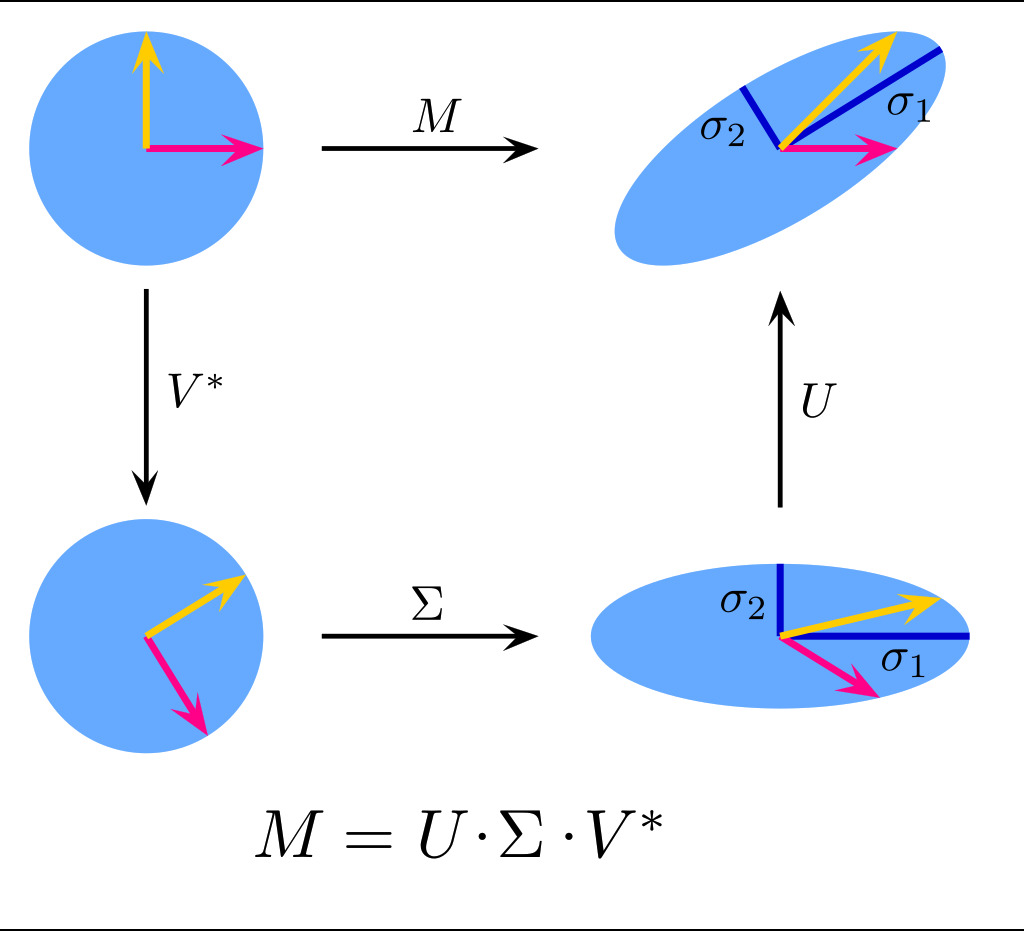
\includegraphics[width=.9\linewidth]{./pics/proc/svd-wiki.jpg}
\end{center}

Our goal is to obtain \[K = v\sigma u^\top.\] Since we only want a
single \(\sigma\) and the number of non-zero singular values is equal to
the rank of the matrix we would like to separate, \textbf{a separable kernel is
a kernel whose rank is equal to \(1\).} In particular, we would obtain

\[K = \sigma_1 u_1 v_1^\top.\]

If \(K\) is not of rank \(1\), we end up with the general case of a
matrix with rank \(r \neq 1\). For this reason, we would obtain

\[ K \approx \sum_{i=1}^r \sigma_i u_i v_i^\top = \sigma_1 u_1 v_1^\top + \sigma_2 u_2 v_2^\top + \dots + \sigma_r u_r v_r^\top,\]
having to perform \(2r\) convolutions, two for each generated pair of
\(u_i\) and \(v_i^\top\).

Why is this convenient? It makes computation cheaper, since instead of
dealing with \(W^2\) operations, now it will be sufficient to precompute
the gradient with \(u_r\) and \(v_r^\top\) only, and those vectors have
size \(W\). Thus, only \(2W\) operations will be needed. However, keep
in mind that if \(r \neq 1\), one has to perform \(2r\) convolutions
with filters having \(W\) size, and sum up everything altogether.
Despite that, the end result will be much better than performing \(W^2\)
operations.

For filters described by a function it is quite the same. Given a filter
\(f(x, y)\) it is said to be separable if

\[f(x, y) = g(x)h(y).\]

An example of a separable filter is the Gaussian filter,

\[\begin{array}{lll} G(x,y;\sigma) & = &\displaystyle  \frac{1}{2\pi \sigma^2}\exp{\left(-\frac{x^2 + y^2}{2 \sigma^2}\right)} = \frac{1}{\sqrt{2\pi} \sigma} \exp{\left(-\frac{x^2}{2\sigma^2}\right)}\frac{1}{\sqrt{2\pi} \sigma} \exp{\left(-\frac{y^2}{2\sigma^2}\right)} \\ & = & g(x)h(y).\end{array}\]

\section{Non-linear operators and other neighborhood operators}
\label{non-linear-operators-and-other-neighborhood-operators}
\subsection{The median filter}
\label{the-median-filter}
A \emph{median filter} is a filter that substitutes each pixel value with the
\textbf{median} of the distribution in the neighborhood. In particular, it
takes all pixels in neighborhood of a given pixel, takes the median of
all those values, and store it in the central pixel. Resulting image
would hopefully see much of its noise being removed by the median filter
(in particular, \emph{shot noise}). Median filter is a non-linear filter.

The median filter is able to address \emph{shot noise}, it's a kind of noise
that strongly affects random, single points in an image.

\subsection{The \(\alpha\)-trimmed mean filter}
\label{the-alpha-trimmed-mean-filter}
An example is the \emph{\(\alpha\)-trimmed mean} filter. Such filter is
designed to remove the \emph{fraction} \(\alpha\) of values in the
neighborhood that are the smallest and the largest.

\subsection{Weighted median filter}
\label{weighted-median-filter}
Too large neighborhood will likely make the filter consider points that
are far from the one in the middle. Basically, we want those points to
count \emph{less} than closer ones, and this is not guaranteed in the classic
median filter (points far from the center of the window are equally
considered). \textbf{Weighted median} filter solves this issue by applying
corresponding weights to pixels. In particular, it corresponds to
solving such optimization problem (for the weighted median \(p = 1\))

\[ \min_{g(i, j)} \sum_{k, l} w(k, l)|f(i + k, j + l) - g(i, j)|^p,\]
with \(w(k, l)\) being the weight associated to the corresponding
\((k, l)\) position in the filter window. \(k\) and \(l\) will range
from value \(-W\) to value \(W\), and \(p\) is equal to \(1\). This
problem means \emph{finding the \(g(i, j)\) that results in the minimum
distance with weights between a point in neighborhood of \(f\) and the
point \(g(i, j)\)}.

By setting \(p=2\) one obtains the \emph{weighted mean} filter (which does
the mean, but weighted by function \(w\)).

\section{Morphology (non-linear)}
\label{morphology-non-linear}
Morphology is basically the set of operations that allows to manipulate
\emph{shapes} in figures.

A shape can be described by an image containing only \(0\) and \(1\),
that's called a \textbf{binary image}. Binary images are actually images having
only two values, and are usually adopted to describe some kind of shape.
A shape could be, for instance, a feature or a set of points that are
detected in an image; those points are then ``mapped'' to another image
(the binary image) which is related to the original image by containing
collected informations on shapes. Basically, a binary image can describe
a shape by identifying it with \texttt{1} and \texttt{0} values.

A binary image is obtained by a non-binary image by applying a
\emph{thresholding operation} \(\theta\) which is non-linear,

\[\theta(f, t) = \left\{\begin{array}{ll} 1 & \mbox{ if } f \geq t\\ 0 & \mbox{ otherwise } \end{array}\right.\]

\begin{center}
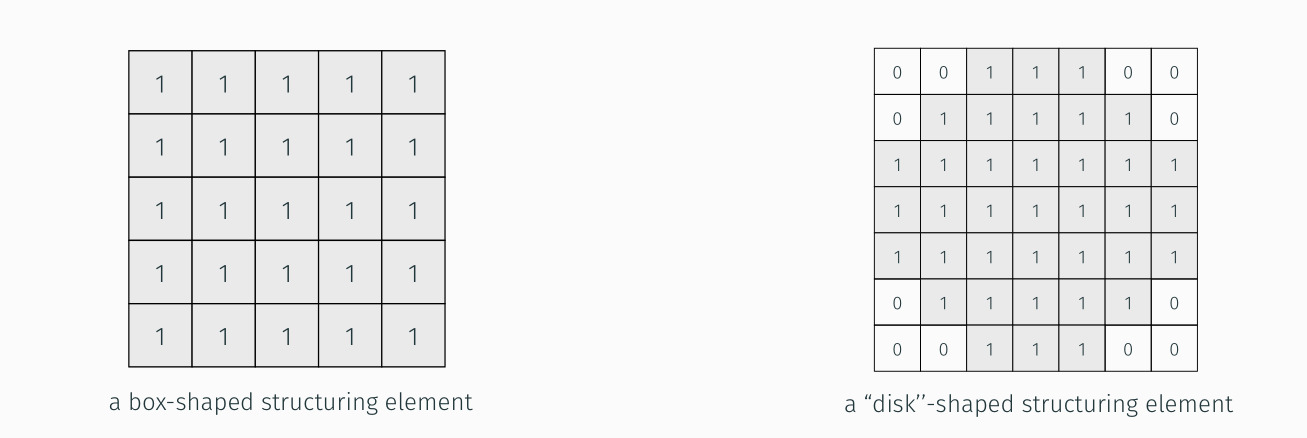
\includegraphics[width=.9\linewidth]{./pics/proc/binary-images.jpg}
\end{center}

Morphological operations consists in two steps,

\begin{enumerate}
\item convolve the image with a \emph{binary structuring element} (e.g. a box
filter);
\item select a binary output, based on the thresholded result of previous
operation.
\end{enumerate}

\subsection{Operations when convolving with shapes}
\label{operations-when-convolving-with-shapes}
There are many possible operations.

Let \(c = f \otimes s\) being the count of the number of \(1\)s falling
inside both figures, the \(f\) image and the \(s\) moving filter
(actually, \(c\) is the count of \(1\)s falling in both \(f\) and \(s\)
because, at each convolution step when calculating each point of the
convolved image \(c\), the pixel value in \(c\) will be the count of
\(1\)s belonging to both functions; this is a peculiar characteristic of
the correlation, since we are dealing with functions whose values are
either \(0\) or \(1\)). Let's also call \(S\) the total number of \(1\)s
in the \(s\) shape. Some operations are

\begin{itemize}
\item \textbf{dilation}, \(\mbox{dilate}(f, s) = \theta(c, 1)\). In this case, a
pixel becomes \(1\) if \emph{at least one \(1\) falls inside both \(f\) and
\(s\), that is when \(f\) and \(s\) intersect} at least a bit. This
happens because the threshold is only \(1\);
\item \textbf{erosion}, \(\mbox{erode}(f, s) = \theta(c, S)\). In this other case,
a pixel becomes \(1\) if \emph{\(f\) and \(s\) are fully-intersected, or
when the entire \(s\) falls inside \(f\)}. This happens because the
threshold is the same of the total numbers of point in shape \(s\),
which is \(S\);
\item \textbf{majority}, \(\mbox{maj}(f, s) = \theta(c, S/2)\).
This operation assigns \(1\) to the center of the filtering window
\(s\) if \emph{the majority of \(s\) falls inside \(f\)}. Basically,
picking a threshold of \(\frac{S}{2}\) means that the result will be
\(1\) if the intersection has \emph{at least} half of the points in shape
\(s\);
\end{itemize}

Combining those operations leads to new operations, for instance

\begin{itemize}
\item \textbf{opening}, \(\mbox{dilate}(\mbox{erode}(f, s), s)\);
\item \textbf{closing}, \(\mbox{erode}(\mbox{dilate}(f, s), s)\),
\end{itemize}

are operations that, respectively, allow opening and closing of holes in
a binary image.

\begin{center}
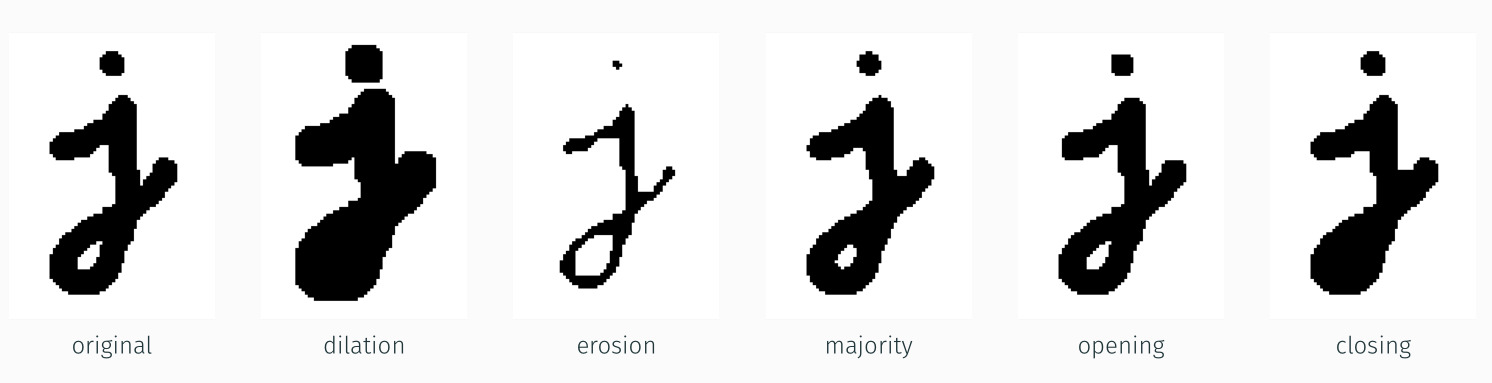
\includegraphics[width=.9\linewidth]{./pics/proc/morphological-operations.jpg}
\end{center}

\subsection{Distance transform}
\label{distance-transform}
\emph{Distance transform} \(D(i, j)\) of a given binary image \(b(i, j)\) and
given a metric \(d\), is a transform such that

\[D(i, j) = \min_{k, l: b(k, l) = 0} d(i-k, j-l).\] Basically, a pixel
value is given by its distance with metric \(d\) from the closest point
whose value is \(0\) (that point is indeed \(b(k, l)\), and it is
indicated by the constraint \(k, l: b(k, l) = 0\)).

Commonly adopted metrics are:

\begin{itemize}
\item 1-norm, which is the \emph{city-block} distance \[d(i, j) = |i| + |j|.\]
\item 2-norm, which is the \emph{Euclidean} distance
\[d(i, j) = \sqrt{i^2 + j^2}.\]
\end{itemize}

Hence, for example in above example when we are in the case of the
city-block distance, one has to minimize the quantity
\[d(i-k, j-l) = |i - k| + |j - l|.\]

\begin{center}
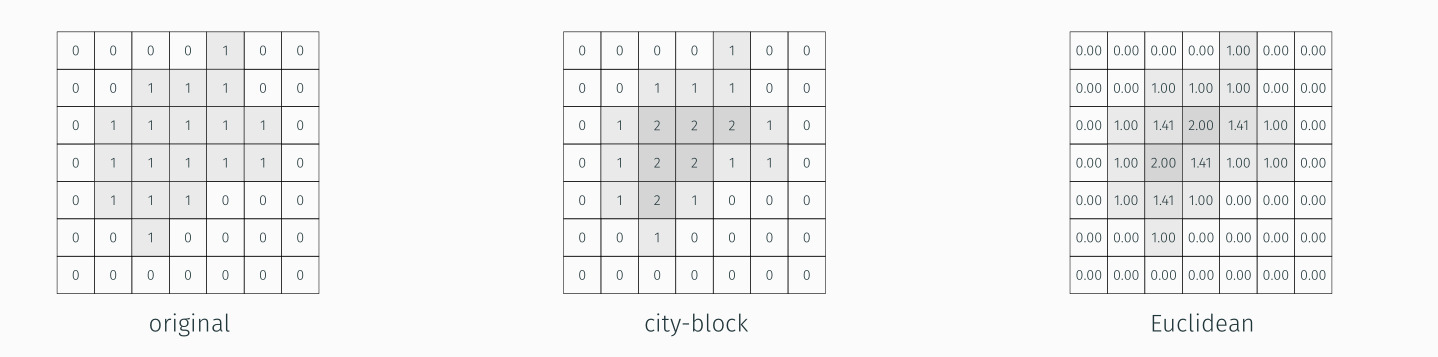
\includegraphics[width=.9\linewidth]{./pics/proc/distance-transform.jpg}
\end{center}

\section{Connected Components}
\label{connected-components}
Connected components of an image are the regions of the image with
adjacent pixels having the same value. Connected components can be
either \emph{labeled} or not, depending on the kind of task we want to
perform.

\begin{center}
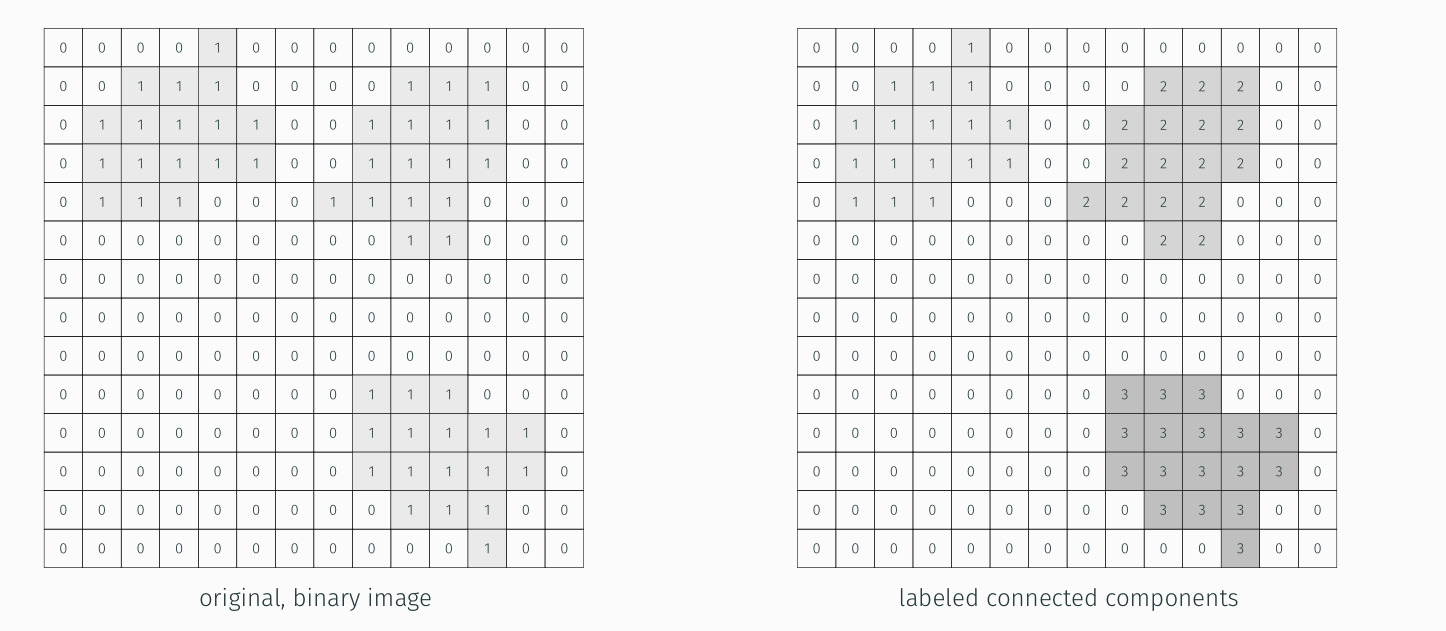
\includegraphics[width=.9\linewidth]{./pics/proc/connected-components.jpg}
\end{center}

Connected components can be described by some quantities. In particular,
we could be interested in:

\begin{enumerate}
\item \emph{area} of the connected components, which is the number of pixels
belonging to a connected component;
\item \emph{perimeter} of the connected components, which is the number of
pixels belonging to the \emph{boundary} of the connected component;
\item \emph{centroid} which has formula
\[(\overline x, \overline y) = \left(\frac{\sum x^{(i)}}{N},\frac{\sum y^{(i)}}{N}\right);\]
\item \emph{matrix of the second moments}, which is
\[I = \begin{bmatrix} I_{xx} & I_{xy} \\ I_{yx} & I_{yy} \end{bmatrix} = \sum_{i=1}^N \begin{bmatrix} x^{(i)} - \overline{x} \\ y^{(i)} - \overline{y} \end{bmatrix} \begin{bmatrix} x^{(i)} - \overline{x} & y^{(i)} - \overline{y} \end{bmatrix};\]
\item \emph{Hu moment invariants}.
\end{enumerate}

\section{Image warping}
\label{image-warping}
\emph{Image warping} is the idea to modify an image by applying some kind of
transformation.

\begin{center}
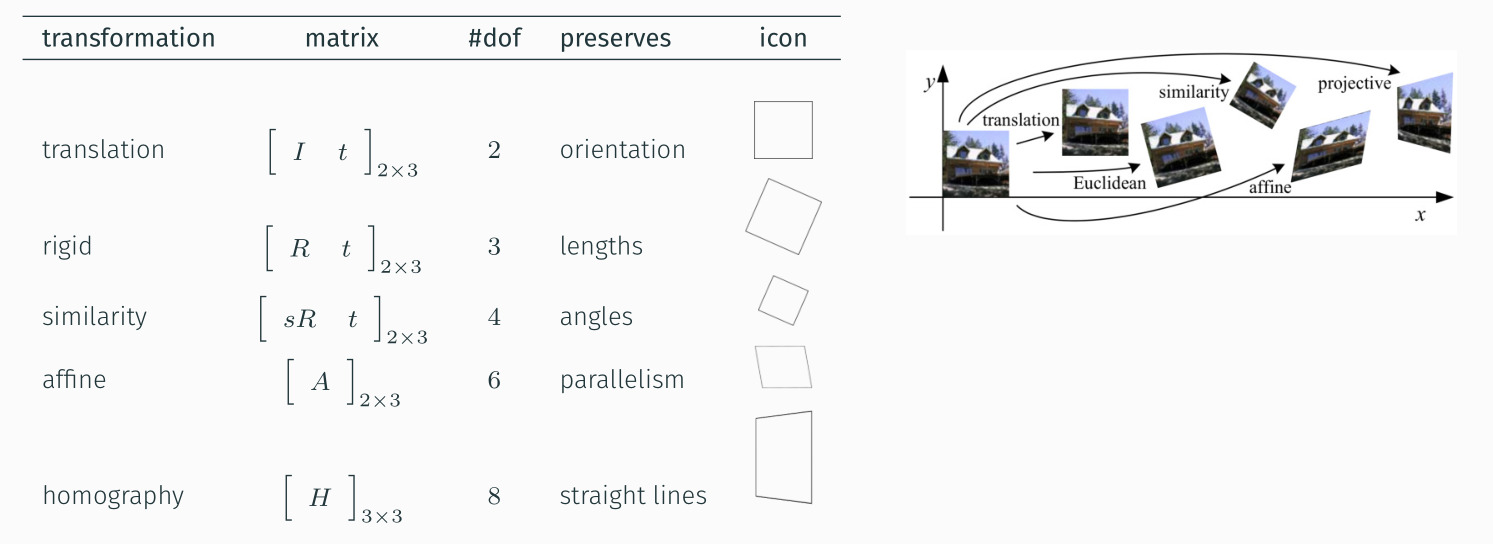
\includegraphics[scale=0.27]{./pics/proc/image-warping.jpg}
\end{center}

The above transformations will change the \emph{domain} of the image, are
\emph{global} and \emph{parametric}. Another example of a parametric
transformation is the \emph{rotation}. There are two kinds of warping: the
\emph{forward warping} and the \emph{inverse warping}.

\subsection{Forward warping}
\label{sec:org9ed9167}
\vspace*{0.6cm}\hrule
\hrule
\hrule
\vspace*{0.4cm}
\begin{quote}
\emph{Forward warping transforms an image \(f(x)\) into an image \(g(x')\) by means of the transform \(x' = h(x)\):}
\end{quote}

\begin{verbatim}
procedure ForwardWarp(f, h) out g
    for each pixel x in f(x) do
        compute the destination x'
        copy pixel f(x) to g(x')
    end for
end procedure
\end{verbatim}
\vspace*{0.6cm}\hrule
\hrule
\hrule
\vspace*{0.4cm}

This works by calculating point in the output image by applying transform of
input pixels. Looks like this works well, but in practice it will not: by
computing destination location \(x'\), one has a non-integer value as a result.
It is not clear how to deal with such values. Basically, what's wrong here is
that we apply a transformation without having guaranteed that the output
location will be an integer (and thus, we cannot locate the resulting
transformed pixel reliably).

\subsection{Inverse warping}
\label{sec:orgb2340b3}
\vspace*{0.6cm}\hrule
\hrule
\hrule
\vspace*{0.4cm}
\begin{quote}
\emph{Inverse warping transforms an image \(f(x)\) into an image \(g(x')\) by means of the transform \(x = h^{-1}(x') = \hat{h}(x)\), with \(x' = h(x)\):}
\end{quote}

\begin{verbatim}
procedure InverseWarp(f, h) out g
    for each pixel x' in g(x') do
        compute the source location x = h^{-1}(x')
        resample image f at location x in order to get f(x) value
        copy pixel f(x) to g(x')
    end for
end procedure
\end{verbatim}
\vspace*{0.6cm}\hrule
\hrule
\hrule
\vspace*{0.4cm}

This works well, because our output is \emph{guaranteed to be an integer}, at
the cost of resampling the \emph{input} in order to find the value of the
pixel before the transformation, and then applying the transform at the
correct location. Resampling requires a well-crafted interpolation
filter, because generally a sampling rate \(r\) is not defined for
\(g(x')\) output image.

\subsection{Non-parametric transforms}
\label{sec:org1af1acf}
\begin{center}
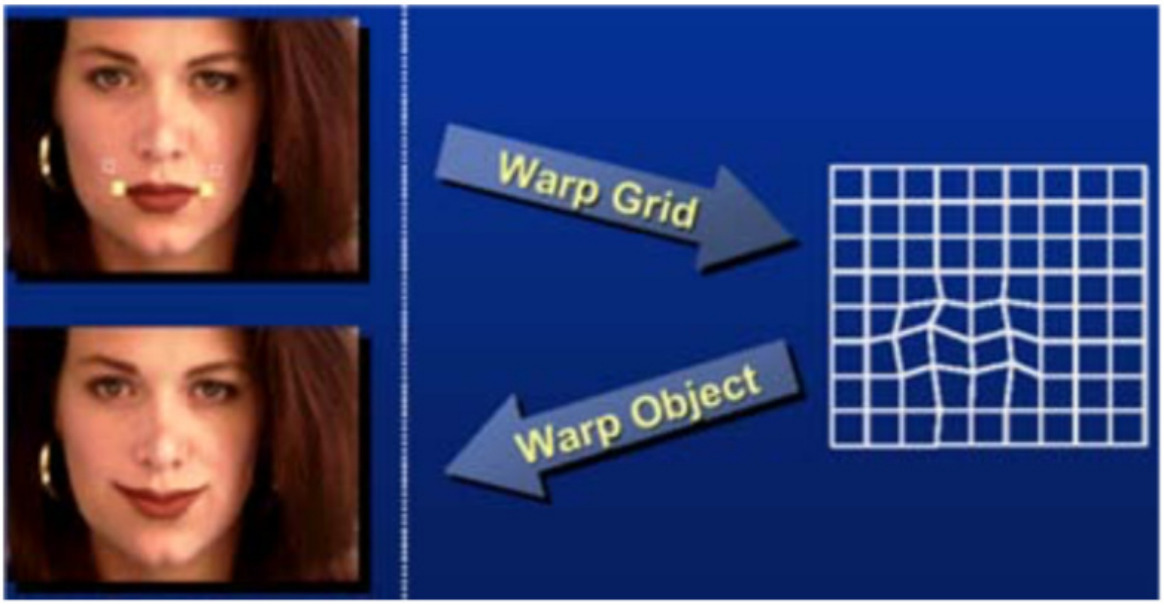
\includegraphics[width=.9\linewidth]{./pics/proc/non-parametric-transform.jpg}
\end{center}

Non-parametric transforms are all those that are non global. Basically,
non-parametric transforms allow to define local transformations whose
amount of transformation is different from place to place.

A common approach to achieve this is to first define a \emph{sparse} set of
corresponding points, then interpolate to a dense displacement field via
triangulation followed by the application of an affine motion.

\section{Multi-resolution representations}
\label{sec:org210d0d7}
\subsection{Upsampling and downsampling}
\label{sec:org5e0c493}
\emph{Upsampling} and \emph{downsampling} are, respectively, increasing and
decreasing the size of an image. Usually, upsampling is useful when the
image needs to match the size of a pre-trained algorithm or the size of
a printer, while downsampling is also required when applying
\emph{coarse-to-fine matching} (starting from a small sized picture, finding
a pattern, and then fine-tuning the match as we increase in image size)
and \emph{fine-to-coarse feature tracking} (find features at fine scales, but
rejecting them if they do not have parents in coarser scales).
Downsampling is also useful when we wish to find a pattern in an image
with a fixed-size template.

\subsection{The upsampling process}
\label{sec:org3c568d0}
Upsampling is basically a correlation between the image and an
\emph{interpolation function} \(h(i, j)\) (interpolation):

\[g(i, j)= \sum_{k, l} f(i, j) h(i - rk, j - rl).\]

\begin{center}
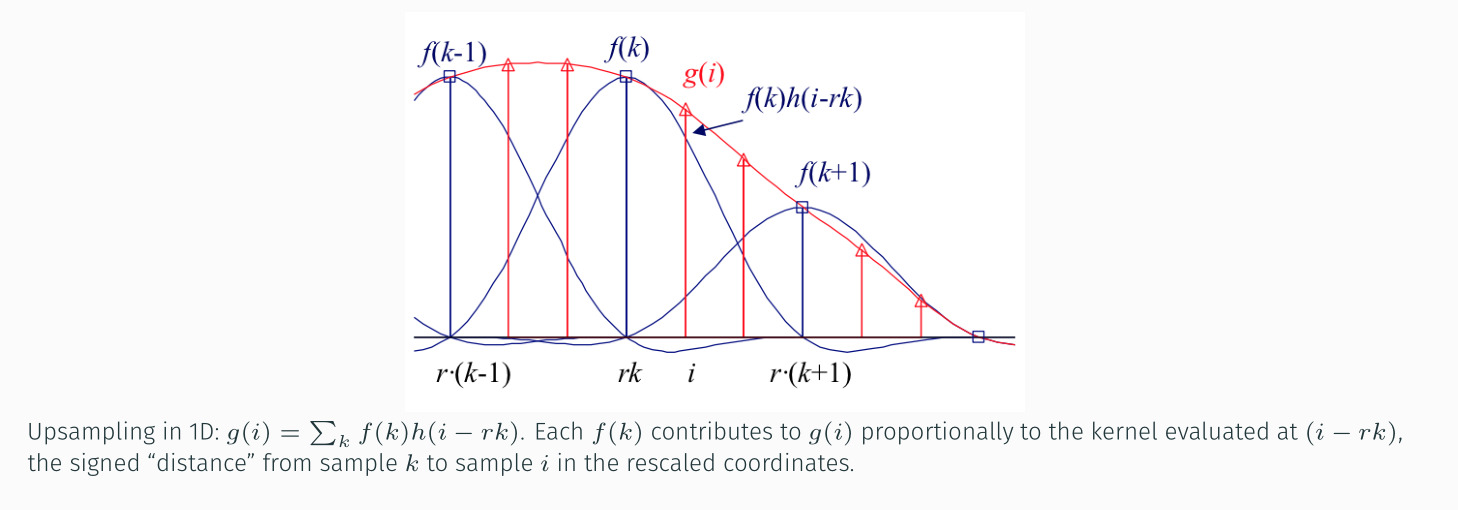
\includegraphics[width=.9\linewidth]{./pics/proc/upsampling.jpg}
\end{center}

We say that \(f\) is the original image, \(h\) is the \emph{interpolation
kernel}, and \(r\) is the \emph{upsampling rate} (the new sampling rate of
the image).

Common interpolation kernels are:

\begin{itemize}
\item \emph{bilinear};
\item \emph{bicubic};
\item the product of two bicubic \href{https://en.wikipedia.org/wiki/Spline\_(mathematics)}{splines}, that is
\end{itemize}

\[h(x) = \left\{ \begin{array}{ll} 1 - (a + 3)x^2 + (a + 2)|x|^3 & \mbox{ if } |x| < 1\\ a(|x| - 1)(|x| - 2)^2 & \mbox{ if } 1 \leq |x| < 2\\ 0 & \mbox{ otherwise } \end{array} \right. \]

with usually \(a = -1\). \(a\) is the derivative at \(x = 1\); setting
it equal to \(-1\) makes our bicubic resemble the
\href{https://en.wikipedia.org/wiki/Sinc\_function}{sinc function} much
more.

\subsection{Aliasing}
\label{aliasing}
\emph{Aliasing} is the phenomenon for which, when sampling a signal, choosing
a too-low sample rate (below the double of the max frequency of the
signal - Nyquist-Shannon theorem) results in an image that is
indistinguishable from sampling to an even lower frequency.

\begin{center}
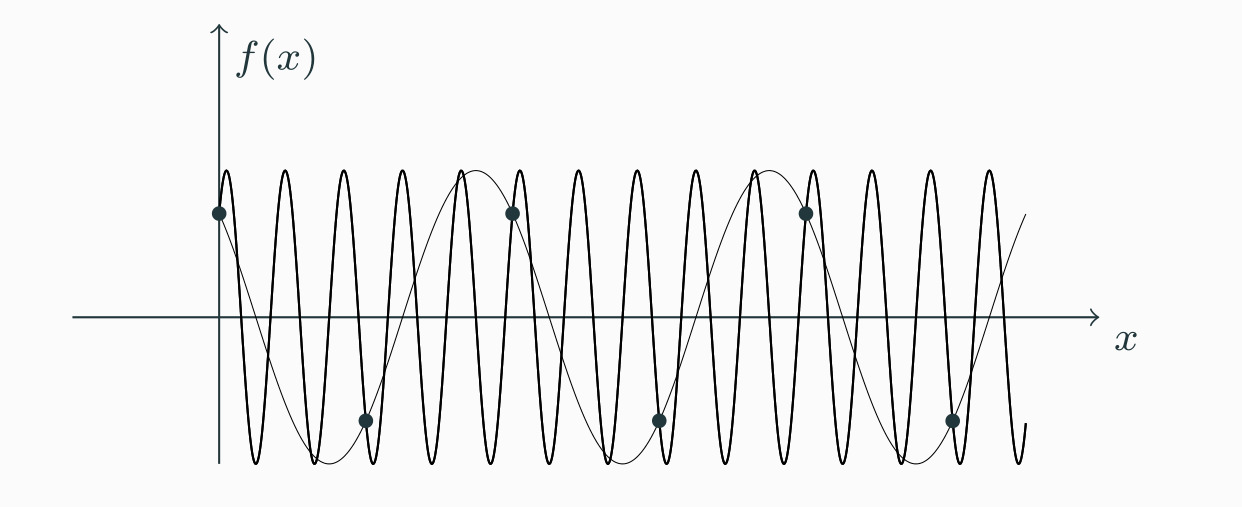
\includegraphics[width=.9\linewidth]{./pics/proc/aliasing.jpg}
\end{center}

When dealing with signals where sampling at enough frequency is
impossible, the only thing left is to low-pass filter: as a consequence,
max frequency of signal would drop and required double of max sampling
frequency will be much lower.

\subsection{The downsampling process}
\label{the-downsampling-process}
Downsampling is a two-step procedure.

First, in order to avoid aliasing a convolution with a low-pass filter
is performed. Second, we simply take one sample every \(r\)-th:

\[g(i, j) = \sum_{k, l} f(k, l)h(ri - k, rj - l).\]

\begin{center}
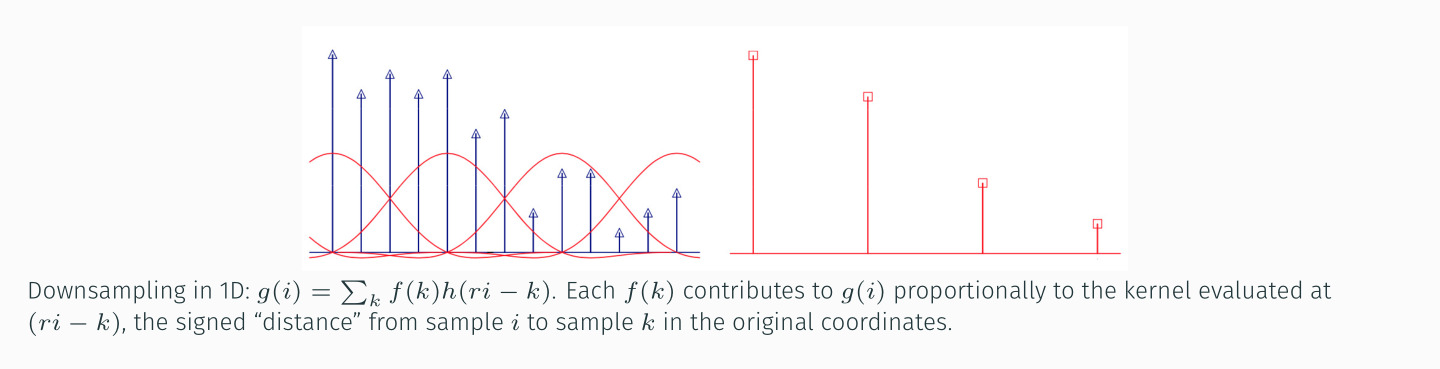
\includegraphics[width=.9\linewidth]{./pics/proc/downsampling.jpg}
\end{center}

\subsection{Multi-resolution representation}
\label{multi-resolution-representation}
The basic idea of multi-resolution representation is that by having many
various-scale representations of a same image at our disposal, each one
of them having more and more coarser details as we are downsampling the
image, we can detect features at many levels of representations with the
same templates. Each level will offer peculiar features at a certain
scale, by investigating each one of them we are able to match and
finally track all features, no matter their scale.

\subsection{Image pyramids}
\label{image-pyramids}
\emph{Image pyramids} are conceptual pyramids obtained by subsequent
downsampling of an original image.

A common pyramid structure is the \emph{octave pyramid}, for which every
image is downsampled at \(r = 2\) rate. Similarly, the \emph{half-octave
pyramid} sees every image downsampled at \(r = \sqrt{2}\).

\begin{center}
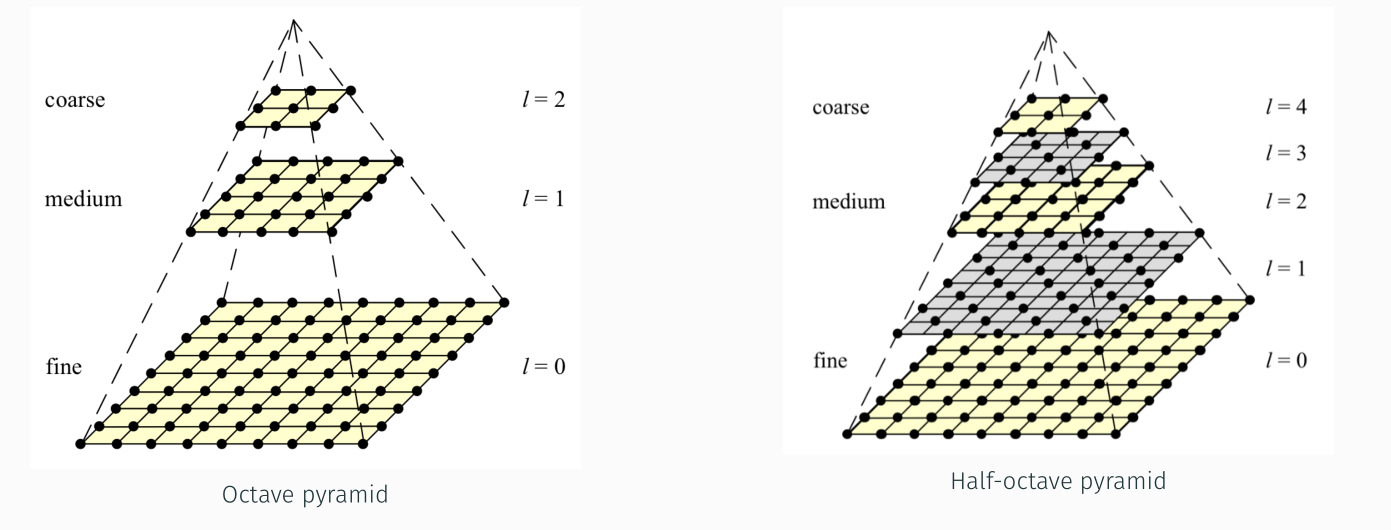
\includegraphics[width=.9\linewidth]{./pics/proc/image-pyramid.jpg}
\end{center}

When downsampling, a smoothing filter should be applied in order to
prevent aliasing. When such filter is a Gaussian, the pyramid is called
\textbf{Gaussian pyramid}.

\chapter{Feature Detection}
\label{feature-detection}
\section{Key-point detection and matching}
\label{key-point-detection-and-matching}
\subsection{Tracking and matching}
\label{tracking-and-matching}
Correspondences between two images can be obtained by \emph{feature
detection}, and then by \emph{finding two features which are very similar
across images}. Such features are, usually:

\begin{itemize}
\item \emph{keypoints}: texture patches surrounding the point location;
\item \emph{edges};
\item \emph{geometric primitives} such as lines, curves, and so on.
\end{itemize}

When it comes to finding features and matching them across images, there
are two approaches.

The first approach is the so-called \textbf{detect-and-track}. By doing
detect-and-track, we are finding features \emph{in a single image} that can
be tracked \emph{by performing a local search}. This is particularly good
when we are dealing with images been taken from nearby viewpoints, or
for video sequences where usually features will ``move'' slowly across
frames.

The second approach is named \textbf{detect-and-match}. In this approach, we
are finding features \emph{in all images}, then matching such features \emph{based
on their local appearance}. This approach is very good when there's a
lot of motion involved, and the two images are taken from a very
different point of view.

\subsection{The feature and matching pipeline}
\label{the-feature-and-matching-pipeline}
Basically, it all boils down to 3 steps:

\begin{enumerate}
\item \emph{feature detection}: some features are extracted from each image,
such features are likely to match well in other images;
\item \emph{feature description}: each extracted feature will be assigned to a
\emph{descriptor}, which is required to be \emph{invariant} to rotation and
illumination;
\item either \emph{feature matching} (searching the same feature in other
images) or \emph{feature tracking} (where the search is restricted to a
small neighborhood of the considered feature).
\end{enumerate}

\section{Harris Corner Detector}
\label{harris-corner-detector}
The core idea of the \textbf{Harris Corner Detector} is that to detect corners,
a necessary condition for a feature is to \textbf{exhibit intensity changes
(gradient)} in at least \emph{two different orientations}. This is due to the
fact that, if change occurs in a single direction, ambiguity occurs.

\begin{center}
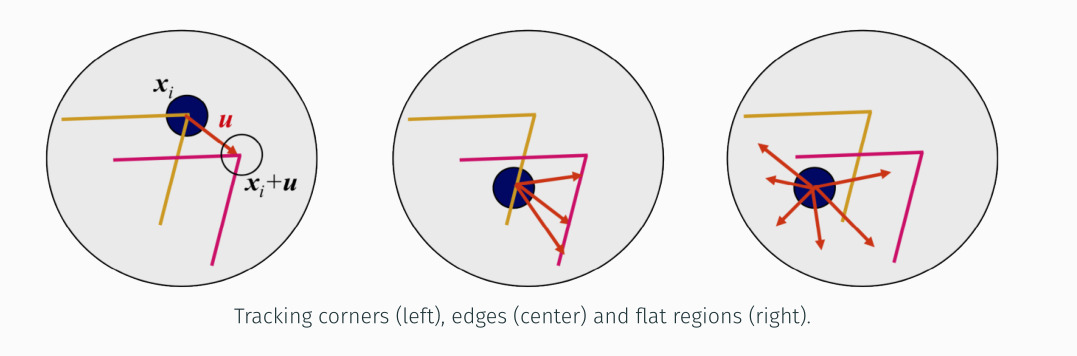
\includegraphics[width=.9\linewidth]{./pics/det/corner-detection.jpg}
\end{center}

Basically, we are going to pick a region of the figure where the
gradient varies in \emph{at least} two directions, and then go track it
across the other images.

\textbf{Harris Corner Detector} works by computing the gradient between two
different (translated) versions of the same window \(W\). Window \(W\)
is centered in pixel \((x, y)\) of image \(I\), and its translated
version is shifted by the quantity \((\Delta x, \Delta y)\). The method
computes the \emph{sum of square differences} by means of the calculus

\[E(x, y, \Delta x, \Delta y) = \sum_{d_x, d_y \in W} [I(x + d_x, y + d_y) - I(x + \Delta x + d_x, y + \Delta y + d_y)]^2,\]

where the \(d_x\) and \(d_y\) denote the indexes of the sum.

Basically, the goal here is to get the gradient. In order to do so, we
employ the Taylor series expansion, truncating it at the first order.
Hence,

\[I(x + \Delta x + d_x, y + \Delta y + d_y) \approx I(x + d_x, y + d_y) + \nabla I(x + d_x, y + d_y)^\top \begin{bmatrix} \Delta x \\ \Delta y \end{bmatrix}.\]

By substituting this term into \(E\), one gets

\[E(x, y, \Delta x, \Delta y) = \sum_{d_x, d_y \in W} \begin{bmatrix} \Delta x & \Delta y \end{bmatrix} \nabla I(x + d_x, y + d_y) \nabla I(x + d_x, y + d_y)^\top \begin{bmatrix} \Delta x \\ \Delta y \end{bmatrix},\]

where the general relationship \[(v^\top u)^2 = u^\top v v^\top u\]
holds, and

\[ \nabla I(x + d_x, y + d_y) \nabla I(x + d_x, y + d_y)^\top = \begin{bmatrix} I^2_x & I_x I_y \\ I_x I_y & I^2_y \end{bmatrix}.\]

Rearranging the equation,

\[\begin{array}{lll}E(x, y, \Delta x, \Delta y) & = & \begin{bmatrix} \Delta x & \Delta y \end{bmatrix} \underbrace{\begin{bmatrix}\displaystyle  \sum_{d_x, d_y \in W} I^2_x & \displaystyle \sum_{d_x, d_y \in W} I_x I_y \\ \displaystyle \sum_{d_x, d_y \in W} I_x I_y & \displaystyle \sum_{d_x, d_y \in W} I^2_y \end{bmatrix}}_{C} \begin{bmatrix} \Delta x \\ \Delta y \end{bmatrix} = \\ & = & \begin{bmatrix} \Delta x & \Delta y \end{bmatrix} C \begin{bmatrix} \Delta x \\ \Delta y \end{bmatrix},\end{array}\]

where \(C\) is \emph{positive semidefinite} by construction.

In order to better obtain a rotationally invariant operator, and to get
a smoother operator it is better to use a Gaussian weighting window for
each term of the \(C\) matrix. Hence, by applying weights

\[w(d_x, d_y) = \frac{1}{2 \pi \sigma^2}\exp{\left(-\frac{d_x^2 + d_y^2}{2\sigma^2}\right)},\]
one finally gets

\[\begin{array}{lll}E(x, y, \Delta x, \Delta y) & = & \begin{bmatrix} \Delta x & \Delta y \end{bmatrix} \underbrace{\begin{bmatrix}\displaystyle  \sum_{d_x, d_y \in W} w(d_x, d_y) I^2_x & \displaystyle  \sum_{d_x, d_y \in W} w(d_x, d_y) I_x I_y \\ \displaystyle  \sum_{d_x, d_y \in W} w(d_x, d_y) I_x I_y & \displaystyle \sum_{d_x, d_y \in W} w(d_x, d_y) I^2_y \end{bmatrix}}_{\hat C} \begin{bmatrix} \Delta x \\ \Delta y \end{bmatrix} = \\ & = & \begin{bmatrix} \Delta x & \Delta y \end{bmatrix} \hat{C} \begin{bmatrix} \Delta x \\ \Delta y \end{bmatrix}.\end{array}\]

The rationale is that the farther away from the centre of the window
(the center of the feature we are going to detect), the lesser the
effect it should have on the \(E\) computation. With this we specify we
want our corner in the middle of the feature, and not anywhere else.

\subsection{Second moment matrix}
\label{second-moment-matrix}
\(\hat{C}\) is called \textbf{second moment matrix}. It is a \emph{symmetric} and
\emph{positive semidefinite} matrix. Since it has such properties, it can be
decomposed into a product between three matrices, the middle one being
the diagonal eigenvalues matrix \(\Lambda\), such as

\[\hat{C} = T \Lambda T^\top = T \begin{bmatrix} \lambda_1 & 0 \\ 0 & \lambda_2\end{bmatrix} T^\top,\]
where the ordering of eigenvalues is such that
\(\lambda_2 > \lambda_1 > 0.\) An interesting property is that for
unitary displacements the sum of squared errors value is constrained by
the eigenvalues, for instance \(\lambda_1 \leq E(x, y) \leq \lambda_2\).
Basically, eigenvalues describe the direction and the intensity of the
gradient in a given window.

There are \(3\) possible cases:

\begin{enumerate}
\item \(\lambda_1, \lambda_2 >> 0\): the feature is a \emph{corner};
\item \(\lambda_2 >> 0\), but \(\lambda_1 \approx 0\): the feature is an
\emph{edge};
\item \(\lambda_1 \approx \lambda_2 \approx 0\): there is \emph{no particular
structure}.
\end{enumerate}

In order to measure how likely a feature is a corner, we may employ
different measures:

\begin{itemize}
\item the \textbf{minimum eigenvalue} \(\lambda_1\);
\item the quantity \(\mbox{det}(\hat{C}) - k \mbox{tr}^2(\hat{C})\);
\item the ratio \(\frac{\mbox{det}(\hat{C})}{\mbox{tr}(\hat{C})}\), which is called \textbf{harmonic mean}.
\end{itemize}

\subsection{General algorithm for Harris corner detector}
\label{general-algorithm-for-harris-corner-detector}
The \emph{Harris corner detector general algorithm} is an algorithm which
takes an \emph{image} as input, and outputs a \emph{position of keypoints}.

Its steps are:

\begin{enumerate}
\item compute \(I_x\) and \(I_y\) by a convolution with derivatives of
Gaussian filter;
\item compute the \(3\) images of the \(C\) matrix, that are
\(I^2_x, I^2_y\) and \(I_x I_y\);
\item convolve each image with a larger Gaussian;
\item compute a scalar index using one of the \(3\) possible measures;
\item throw away noise by finding a local maxima above a certain threshold.
\end{enumerate}

\section{Hessian detector}
\label{hessian-detector}
The \textbf{Hessian detector} has generally the same goals of the Harris corner
detector, with the difference that it employs second derivatives (the
Hessian matrix) in order to do so, and the perks that it is more
responsive on regions with strong texture variation. Basically, the
Hessian matrix is the matrix

\[H(x, y) = \begin{bmatrix} I_{xx} & I_{xy} \\ I_{yx} & I_{yy}\end{bmatrix}.\]

The idea is to detect locations that exhibit \emph{high curvature in two,
orthogonal, directions}.

Hessian detector works by detecting local maxima of \(|\mbox{det}(H)|\)
that are above a certain threshold \(\theta\), by detecting locations
that exhibit \emph{high curvature in two, orthogonal, directions}.

\subsection{Details of Second Moment Matrix}
\label{details-of-second-moment-matrix}
With computations like the Harris detector case, one gets

\[E(x, y, \Delta x, \Delta y) = \begin{bmatrix} \Delta x & \Delta y \end{bmatrix} \hat{C} \begin{bmatrix} \Delta x \\ \Delta y \end{bmatrix},\]
so that \(E\) is as large as possible in all directions of vector
\(\begin{bmatrix} \Delta x \\ \Delta y \end{bmatrix}\). \(\hat{C}\) is
now defined as the \emph{weighted sum of matrices}

\[\hat{C} = \sum w(d_x, d_y) \begin{bmatrix} I^2_x & I_x I_y \\ I_x I_y & I^2_y \end{bmatrix}.\]

Each matrix in the sum are positive semidefinite and symmetric and will
satisfy property
\[\mbox{tr}(\hat C) \geq 0 \Rightarrow \lambda_1 + \lambda_2 \geq 0,\]
and property
\[\mbox{det}(\hat C) = 0 \Rightarrow \lambda_1 \lambda_2 = 0;\] hence,
one eigenvalue is \(0\), the other one can be either \(0\) or greater
than \(0\).

\begin{center}
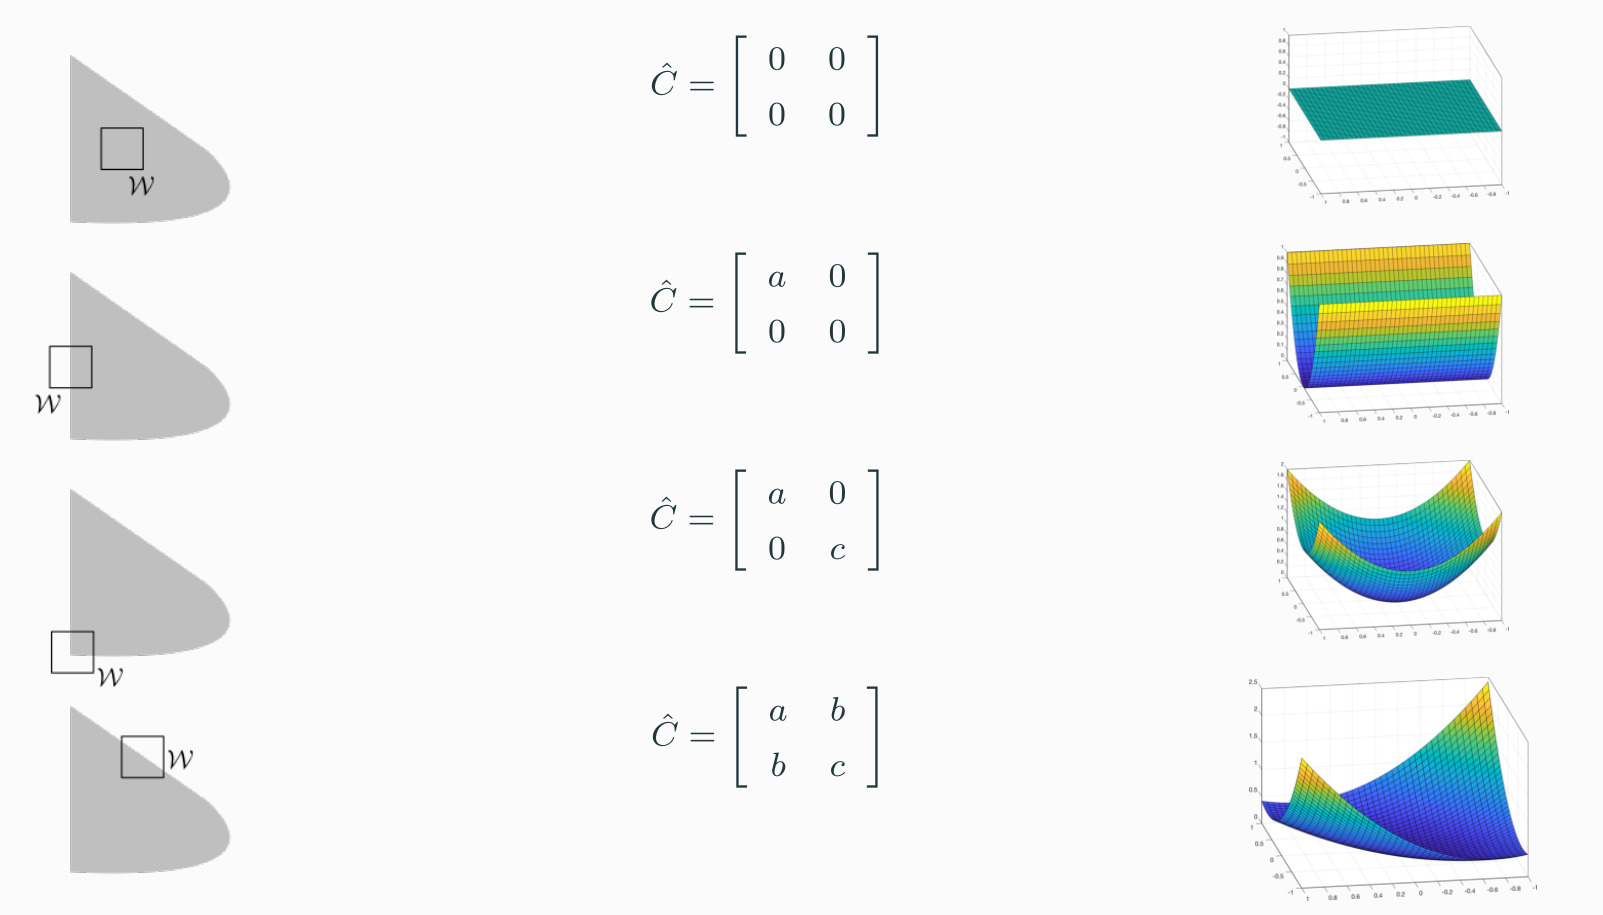
\includegraphics[width=.9\linewidth]{./pics/det/second-moment-matrix-plots.jpg}
\end{center}

\subsection{Second moment matrix to obtain eigenvalues}
\label{second-moment-matrix-to-obtain-eigenvalues}
Lete's consider the property for which the second moment matrix is
orthogonally similar to a diagonal matrix (can be diagonalized by
applying rotation \(T\)),

\[\hat{C} = T\begin{bmatrix}\lambda_{max} & 0 \\ 0 & \lambda_{min}\end{bmatrix}T^\top = \begin{bmatrix} t_{max} & t_{min}\end{bmatrix}\begin{bmatrix}\lambda_{max} & 0 \\ 0 & \lambda_{min}\end{bmatrix}\begin{bmatrix} t_{max}^\top \\ t_{min}^\top \end{bmatrix},\]

where we substituted
\(T = \begin{bmatrix} t_{max} & t_{min}\end{bmatrix}.\) For unitary
displacements, one gets
\(t = \begin{bmatrix} \Delta x & \Delta y \end{bmatrix}^\top\), with
norm \(||t||_ 2 = 1\).

The column \(t_{max}\) of matrix \(T\) represents \emph{the direction along
with \(E\) is maximal, and equal to \(\lambda_{max}\)}. So, in order to
compute the max eigenvalue one could multiply \(\hat{C}\) by the
quantity

\[\begin{array}{lll}t_{max}^\top \hat{C} t_{max} & = & \begin{bmatrix}t_{max}^\top t_{max} & t_{max}^\top t_{min}\end{bmatrix} \begin{bmatrix} \lambda_{max} & 0 \\ 0 & \lambda_{min}\end{bmatrix}\begin{bmatrix} t_{max}^\top t_{max} \\ t_{max}^\top t_{min}\end{bmatrix} = \\ & = & \begin{bmatrix}1 & 0\end{bmatrix} \begin{bmatrix} \lambda_{max} & 0 \\ 0 & \lambda_{min}\end{bmatrix}\begin{bmatrix} 1 \\ 0\end{bmatrix} = \lambda_{max}.\end{array}\]

\(\lambda_{min}\) can be obtained by multiplying by \(t_{min}\).

\subsection{Invariance and covariance to a transform}
\label{invariance-and-covariance-to-a-transform}
The concepts of \textbf{invariance} and \textbf{covariance} are quite similar, despite
being different in some core aspects.

As a general rule, keypoint locations should be both \emph{invariant} to photometric
transformations and \emph{covariant} to geometric transformations.

\begin{itemize}
\item \textbf{invariance}: the image is transformed and keypoint locations \emph{do not
change};
\item \textbf{covariance}: the image is transformed, and keypoint locations \emph{are
transformed accordingly}. Basically, \emph{the regions detected after
having applied a transformation should remain the same as the
transformed versions of the regions which are detected in the original
image}. This means that a transformation should ``transform'' region
detection as well.
\end{itemize}

Harris corner detector already provides covariance to rotation, since
both trace and determinant are invariant to rotation (more generally,
one has to design detectors which are rotationally invariant, so that
they equally respond to same features in both original image and rotated
version.

\section{Scale-space representation}
\label{scale-space-representation}
Some features that appear in a scale may not appear in other scales. For
instance, a corner could be detected in a large-enough scale, but not
being detected at a smaller scale. This happens because we are using the
same strategy of detecting feature at both scales, and features may not
be fit for detection at any scale.

When no a priori knowledge is exploitable, the best idea is to deal with
different scales at the same time. The idea is to provide our algorithms
\emph{many} rescaled versions of the same image, in order to multiply the
chance of finding a given feature at a proper scale.

In order to do so, there are 2 distinct approaches, the straightforward
one being building a pyramid of an image and then looking at a feature
at all scales. However, a better approach is to look for features that
are stable and strong in \textbf{both location and scale}. This leads to a
convenient 'three-dimensional' representation of an image, the
\textbf{scale-space representation}.

\subsection{The scale-space representation}
\label{the-scale-space-representation}
In \textbf{scale-space representation} the goal is to offer the same
'interface' to both location in an image and scale of an image. This is
built by constructing a 3D 'cube' of images, where two dimensions are
represented by the two axis that determine the location of a point in an
image, and the third dimension is \textbf{the scale of the image, with an
ordering}. Basically, we achieve this by subsequently convolving the
image with a Gaussian filter with width \(t = \sigma^2\): each time we
apply the filter, a new smoothed image is born, and we stack it on top
of our scale-space cube. In the end, we will obtain a cube with three
dimensions, \(x, y\) and \emph{scale parameter} \(t\): each point
\((x, y, t)\) represents a triplet in the scale-space.

In practice, each element of the scale-space representation (a 'level'),
has formula

\[L(x, y, t) = G(x, y; \sqrt{t}) * f(x, y).\] Adopted Gaussian filters
are built so that
\[G(x, y; \sqrt{t}) = \frac{1}{2\pi t}\exp{\left(-\frac{x^2 + y^2}{2t}\right)}.\]
If we build a scale-space this way, we will end up with a 'cube' of
images, where going 'up the cube' will correspond to getting more and
more blurred images.

The \emph{principle of scale selection} is the idea that, if we assume that
we are able to detect features at a given scale as spatial local maxima
of derivatives, such features \textbf{may be detected in the same location at
different scales too, with the same combination of derivatives}. With
this approach we basically detect features in both location in image and
scale-space.

Before applying this method, we must \textbf{normalize} derivatives, since
performing those at various scales will yield derivatives with different
strength, possibly rendering our search of a maxima without
normalization meaningless.

\subsection{Derivative normalization}
\label{derivative-normalization}
Derivative normalization should take in account that features that have
intrinsic scales should offer a local maxima of the combination of
derivatives at a given scale.

\begin{center}
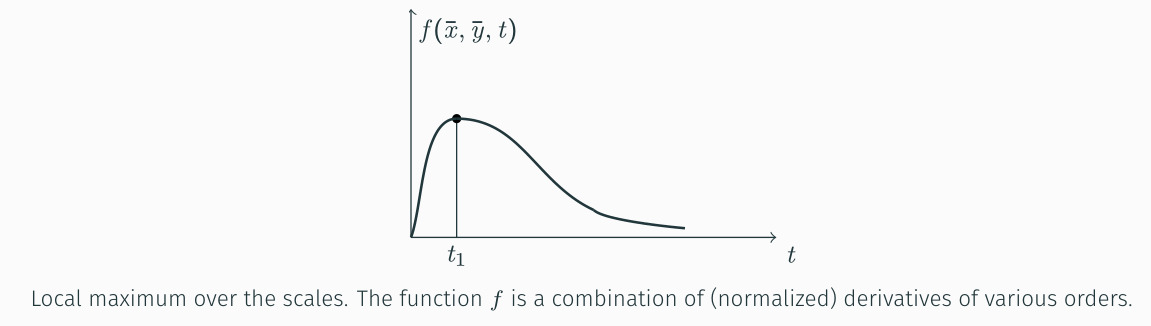
\includegraphics[width=.9\linewidth]{./pics/det/derivative-normalization.jpg}
\end{center}

Normalization generally depends on the kind of feature that has to be
detected. For instance, let's normalize plain sinusoidal functions, such
as \[ g(x) = \sin{\omega_0 x}.\] In our example, convolving a sin with a
Gaussian one obtains

\[L(x, t) = e^{-\frac{\omega_0^2 t}{2}}\sin{\omega_0 x}\] due to a
convolution property. Since there is a decreasing exponential term,
\(L\) will decrease exponentially as we get to a higher scale \(t\). If
we maximize with respect to \(x\), at each scale we get
\[L_{max}^x (t) = e^{-\frac{\omega_0^2 t}{2}},\] which depends on scale
only. The same happens when we apply a \(m\)-th order derivative, which
is

\[L^m(x, t) = e^{-\frac{\omega_0^2 t}{2}}\frac{d^m \sin{\omega_0 x}}{dx^m},\]
which yields a maximum of
\[L^{x^m}_ {max}(t) = \omega_0^m e^{-\frac{\omega_0^2 t}{2}}.\]

Take a look on the result: none of the \(m\)-th derivatives have a local
maximum, since each of them is composed by an exponential that is
constantly decreasing with no maxima.

The trick is in the normalization, that should be good enough to
transform such expressions in expressions that have a local maximum,
preferably in \(\frac{2\pi}{\omega_0}\) (the characteristic length of
the sine wave).

In order to get maxima, we employ the \textbf{\(\gamma\)-normalized derivative
operator} \(t^\gamma \partial x,\) which is perfectly suited for
normalizing derivatives in scale-space representation. Such operator
corresponds to a change of variable \(\xi = \frac{x}{t^{\gamma/2}}.\)
The result will be the non-monotonic behavior we are looking for,

\[ L^{\xi^m}_ {max} (t) = t^{m\gamma/2}\omega_0^m e^{-\frac{\omega^2_0 t}{2}}.\]
Introduction of this change of variable had the result of getting a
unique maximum at \[t_{max} = \frac{\gamma m}{\omega_0^2},\] whose
location across scales is a function of \(\omega_0\) (changing it will
modify the characteristic length of the sine wave, hence the location of
maximum).

\begin{center}
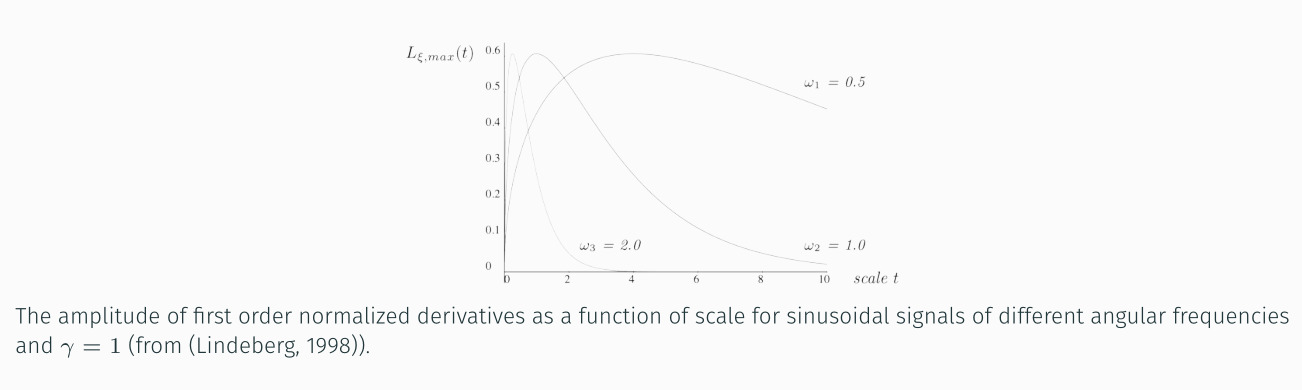
\includegraphics[width=.9\linewidth]{./pics/det/amplitude-normalization.jpg}
\end{center}

The parameter of our normalization is \(\gamma\). Its value will
basically have to be selected depending on the feature that should be
detected.

\subsection{Blob detection}
\label{blob-detection}
Blobs are particular 'circular' configurations that can be commonly
detected by a LoG (Laplacian of Gaussian) filter, which is not oriented,
band-pass, scale-specific (dark blobs of scale \(\sqrt{2}\sigma\) have
strong response) filter with center-surround response.

Recall the formula

\[\nabla^2 G(x, y; \sigma) = \left(\frac{x^2 + y^2}{\sigma^4} - \frac{2}{\sigma^2}\right) G(x, y; \sigma).\]

The LoG can also (erroneously) detect ridges that by chance have the
proper size that may result in a strong response.

The corresponding multi-scale approach to blob detection can be achieved
in \(2\) steps:

\begin{enumerate}
\item compute the scale-space normalized LoG of the image by means of

\[ \nabla^2_{\mbox{norm}} L(x, y, t) = t\nabla^2 G(x, y; \sqrt{t}) * f(x, y),\]
which corresponds to a \(\gamma\)-normalized derivative operator
having \(\gamma=1\) and \(m=2\);

\item find the local extrema in the scale-space (by searching for it in
\textbf{both space and scale}).
\end{enumerate}

Since both scale and space are discrete, one usually has to perform a
search in a local neighborhood window of a given size (for example, a
cubic window of size \(3 \times 3 \times 3\)). A local extrema will
occur in a given scale: that scale is called \emph{characteristic scale}.

This approach both guarantees \textbf{scale covariance} and \textbf{rotational
covariance} since the LoG filter has rotational covariance and in the
scale-space representation it can be shown that scale covariance holds.

\section{The SIFT detector}
\label{the-sift-detector}
\textbf{SIFT} takes its name from the acronym \emph{Scale Invariant Feature
Transform}. SIFT has some interesting characteristics, for instance

\begin{itemize}
\item it uses \textbf{Differences of Gaussians} (we will call them DioG in these
notes) to approximate LoG operator;
\item it uses a \textbf{pyramid} with sub-octave resolution as scales, with
undersampling at each octave; it detects local extrema at \textbf{sub-pixel}
and \textbf{sub-scale} level, by fitting a quadratic function of
\(\Delta x, \Delta y\) and \(\Delta \sigma\) to a raw scale-space
location, and setting its gradient to zero;
\item it \textbf{removes potential edges and ridges} by means of the Hessian matrix of DoG.
\end{itemize}

\subsection{SIFT operations}
\label{sift-operations}
SIFT works by calculating Differences of Gaussians, which approximate
Laplacian of Gaussians at different scales. This is easily done because

\[\frac{\partial G}{\partial \sigma}(x, y, \sigma) = \sigma \nabla^2 G(x, y, \sigma)\]

and therefore by substituting the derivative with the difference
quotient one gets

\[\frac{G(x, y; \sigma + \Delta \sigma) - G(x, y; \sigma)}{\Delta \sigma} \approx \sigma \nabla^2 G(x, y, \sigma)\]

which basically means that a Laplacian of a Gaussian, multiplied by a
\(\sigma\), is well-approximated by a difference of two Gaussians, one
taken at scale \(\sigma\) and the other one at scale
\(\sigma + \Delta \sigma\) (and then dividing by \(\Delta \sigma\)).

If we rename \(k\sigma := \sigma + \Delta \sigma\) we get that
\(\Delta \sigma = (k - 1)\sigma\), therefore one obtains

\[G(x, y; k\sigma) - G(x, y; \sigma) \approx (k-1)\sigma^2 \nabla^2 G(x, y;\sigma) = (k-1)\nabla^2_{\mbox{norm}}G(x, y;\sigma).\]

It practically means that by taking DoG (differences of Gaussians)
instead of Laplacian of Gaussians one has a decent approximation of LoG
while \emph{incorporating normalization} (the closer \(k\) gets to \(1\), the
better the approximation is). In a multi-scale framework, a convenient
choice is \(k=\sqrt[n]{2}\) in order to get \(n\) levels per octave.
SIFT employs \(n = 4\) to get \(4\) levels per octave.

\begin{center}
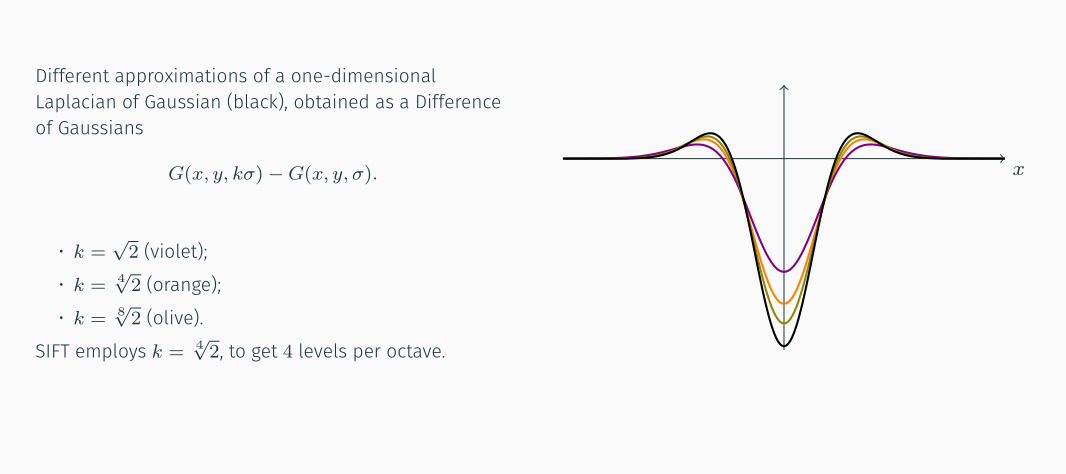
\includegraphics[width=.9\linewidth]{./pics/det/difference-of-gaussians.jpg}
\end{center}

Another important characteristic of the SIFT detector is the \textbf{pyramid}
it employs.

Scales are chosen at sub-octave resolution, with undersampling that
occurs at each octave. For each octave of the scale space, the initial
image is repeatedly convolved with Gaussians in order to produce the set
of scale space images shown on the left in Figure. Adjacent Gaussian
images are subtracted to produce the Difference of Gaussians on the
right. Basically, in order to get the images convolved with
DiffOfGaussians one has to pick two images of adjacent scales
(\(\sigma\) and \(k\sigma = \sigma + \Delta \sigma\)) and perform the
difference. This way we get DioG which is an approximation of LoG. After
each octave, a downsampling by factor of \(2\) occurs: the process is
then repeated.

In order to search the extrema in \(n\) levels per octave one needs
\(n+2\) DioG images, thereby \(n+2+1=n+3\) Gaussian filtered images are
needed.

\begin{center}
\includegraphics[width=.9\linewidth]{./pics/det/sift-scale-space.jpg}
\end{center}

\subsection{Sub-pixel precision}
\label{sub-pixel-precision}
Sub-pixel precision and sub-scale precision are one of the
characteristic features of the SIFT detector. Since at-pixel and
at-scale precision are not enough, one has to perform an \emph{interpolation}
in order to avoid discretization and detect extrema at sub-pixel and
sub-scale level.

The reason why this works is that, by chance, an extrema may not be
\emph{exactly} on a given scale or a given pixel. Reasonably, an extrema will
fall \emph{between} pixels and \emph{between} scales. In order to catch them,
sub-pixel and sub-scale precision is required.

SIFT detects local extrema at sub-pixel and sub-scale level by \emph{fitting
a quadratic function} of \(x, y,\) and \(\sigma\) to the standard 'raw'
scale-space and setting its gradient to \(0\) (this way, an extrema can
detected \emph{between} pixels and scales).

Let \(D(x, y, \sigma)\) denote the \textbf{DioG approximation} of the
normalized Laplacian at scale \(\sigma\) (a convenient notation for
DioG), in the neighborhood of a pixel-level local extremum. By means of
the Taylor expansion at such location,

\[D(x + \Delta x, y + \Delta y, \sigma + \Delta \sigma) \approx D(x, y, \sigma) + [\nabla D(x, y, \sigma)]^\top \Delta + \frac{1}{2}\Delta^\top H(x, y, \sigma) \Delta,\] where \(\Delta = \begin{bmatrix}\Delta x & \Delta y & \Delta \sigma \end{bmatrix}^\top\).

The above representation is a \textbf{quadratic function of \(\Delta\)} (our
interpolation function).

This means that the gradient of \(D\) and the Hessian matrix can be
approximated by differences of neighboring sample points. By setting the
sum at zero, one can obtain extrema at sub-scale and sub-pixel level,

\[ \nabla D (x, y, \sigma) + H(x, y, \sigma)\Delta = 0,\] and one gets
as solution

\[\Delta = -H^{-1}(x, y, \sigma) \nabla D(x, y, \sigma).\]

\subsection{SIFT to detect edges and ridges}
\label{sift-to-detect-edges-and-ridges}
Poorly defined peaks can happen when using DioG. In particular, ridges
and edges can result in unwanted strong responses. In order to avoid
this behavior, SIFT employs Hessian matrix of DioG computed in
correspondence of the location \((x, y, \sigma)\) of the keypoint.
Basically, a rejection criterion
\(r = \frac{\alpha}{\beta} > \overline{r}\) between maximum and minimum
eigenvalue (respectively, \(\alpha\) and \(\beta\)) is adopted. Since
\[\frac{\mbox{det} H}{\mbox{tr}^2 H} = \frac{\alpha \beta}{(\alpha + \beta)^2} = \frac{\beta^2 r}{\beta^2(r + 1)^2} = \frac{r}{(r + 1)^2}\]
is monotonic with respect to \(r\), the peak is rejected when
\[\frac{\mbox{det} H}{\mbox{tr}^2 H} \geq \frac{\overline{r}}{(\overline{r} + 1)^2}.\]

\subsection{SIFT descriptor}
\label{sift-descriptor}
A \textbf{SIFT descriptor} associated to a keypoint is a \textbf{histogram of the
gradient orientation} in the neighborhood of the keypoint.

Given (for instance) a total of \(8\) directions for the gradient, the
histogram will contain the gradient value computed in all those \(8\)
directions in a given pixel. The number of pixels in a given histogram
must be chosen.

Orientation of keypoints can be computed by means of the SIFT descriptor
(a histogram containing information on gradient for each pixel belonging
to the keypoint).

To achieve scale invariance, SIFT considers a fixed window of
\(16 \times 16\) in the pyramid level in which the keypoint has been
detected.

To achieve rotation invariance, a \textbf{dominant orientation} should be
computed:

\begin{enumerate}
\item the gradient is computed for each pixel of the window;
\item a histogram of \(36\) angular bins is built, where the contribution
to each bin is weighted by the gradient magnitude and a Gaussian
centered in the window (in order to make far pixels less important);
\item the dominant orientation is the mode of the histogram;
\item in order to increase the angular resolution, the mode is estimated by
quadratic interpolation with the two neighboring bins;
\item the histogram is \emph{multi-modal} only when there are local maxima of
the histogram within the \(80\%\) of the mode (local maxima should be
high enough to have a peak that is \(\frac{4}{5}\) the value of the
mode). A descriptor is then generated for each dominant orientation.
\end{enumerate}

Given the dominant orientation, a \emph{descriptor} can be constructed as
follows:

\begin{enumerate}
\item a \(16 \times 16\) window, rotated according to the dominant
orientation is considered at the same level of detection;
\item a Gaussian-weighted gradient is computed for each pixel;
\item the window is then divided into \(16\) subwindows, each having size
\(4\times 4\);
\item a \(8\) bin histogram of orientation is constructed. The weighting of
each bin is performed by gradient magnitude.
\end{enumerate}

This process finally leads to a \(128\) non-negative values that should
be collected into a vector. The vector is then normalized to unit length
(in order to achieve \emph{contrast invariance}). Finally, values below a
certain threshold (SIFT employs a threshold of \(0.2\)) are trimmed to
zero, and the vector is, again, normalized.

The result of this entire process is the \textbf{SIFT descriptor} for a given
keypoint.

\begin{center}
\includegraphics[width=.9\linewidth]{./pics/det/sift-keypoints.jpg}
\end{center}

\subsection{Steerable filters as compact descriptors}
\label{steerable-filters-as-compact-descriptors}
The \textbf{steerable filters} can be adopted as a compact descriptor in the
sense that instead of describing a keypoint with all filters, one could
use steerable filters in order to lower the number of filters.

\begin{itemize}
\item The descriptor is \emph{compact} because it is composed of the filter
responses which correspond to filters centered in the keypoint. Hence,
\(n\) filters will result in a descriptor of size \(n\);
\item in order to compute derivatives up to the \(4\)-th order, \(16\)
filters are required - however, only \(14\) are necessary, since two
couples of filters are the same with different orientation; they are
suitable for representing even (ridge-type) features; they are the
most effective among the short length descriptors.
\end{itemize}

\subsection{Feature matching}
\label{feature-matching}
In \emph{feature matching} step, features are matched across pair of images.
To prevent false positive matches, one has to implement some tricks
based on \textbf{distancing}.

\subsection{Distance in matching strategies}
\label{distance-in-matching-strategies}
To prevent too many false positives matches across images we assume that
correctly matching features should be very close each other. In
particular, we employ a \textbf{distance between descriptors}, such as

\[d(D_A, D_B) = \sqrt{(D_A, D_B)^\top W (D_A, D_B)}, \] where \(W\) is a
semidefinite positive matrix that acts as a weight (weighted distance).
In some cases, one simply removes \(W\), obtaining an Euclidean distance
between descriptors. In some other cases, especially when descriptors
are histograms, one could employ a much more complex distance known as
\textbf{Earth Mover's Distance} (EMD).

Simply calculating distance value means nothing. One has to put down a
rule in order to decide if two features are to be matched. In
particular, let \(D_A\) being the feature to match, there are three
different approaches:

\begin{enumerate}
\item \textbf{fixed threshold}: simply putting, if \(d(D_A, D_B) > \theta\) those
features are not matched (matching occurs when
\(d(D_A, D_B) \leq \theta\));
\item \textbf{nearest neighbor}: simply match the nearest neighbor in the feature
space. Some features may not have matches, so a threshold is still
adopted to reduce the number of wrong matches;
\item \textbf{Nearest Neighbor Distance Ratio (NNDR)}: let \(D_B\) and \(D_C\),
respectively, the closest and the second closest neighbors of \(D_A\).
By heuristic \[NNDR = \frac{d(D_A, D_B)}{d(D_A, D_C)}\] one obtains
an index that measures the ratio between the two closest neighbors of
a given feature, in order to correctly match. A threshold is then
applied to reject ratios above a certain threshold.
\end{enumerate}

\begin{center}
\includegraphics[width=.9\linewidth]{./pics/det/matching-strategies.jpg}
\end{center}

\subsection{Issues in matching phase}
\label{issues-in-matching-phase}
Matching can bring false positives. Moreover, matching may be not
efficient. Consider the case where we decide to compare all features
against all other features, in each pair of potentially matching images.
This is quadratic in the number of extracted features, so it is
impractical in most applications. One should adopt more efficient data
structures and algorithms.

\subsection{SIFT overall algorithm}
\label{sift-overall-algorithm}
The overall algorithm is as follows,

\vspace*{0.6cm}\hrule
\hrule
\hrule
\vspace*{0.4cm}

\textbf{Input:} image

\textbf{Output:} position, scale and orientation of keypoints

\begin{enumerate}
\item compute the Gaussian pyramid
\item compute DioG by subtracting nearby levels of the same octave
\item find scale-space extrema at pixel level
\item adopt interpolation to refine location in scale-space (sub-pixel and
sub-scale precision)
\item reject extrema with absolte valute below a certain threshold
\item reject extrema corresponding with edges, based on the ratio between
maximum and minimum eigenvalues of the Hessian matrix
\item compute dominant orientation of the keypoints, by histogram of
gradients
\end{enumerate}

\vspace*{0.6cm}\hrule
\hrule
\hrule
\vspace*{0.4cm}

\section{Edge detection}
\label{edge-detection}
Edges are spatially rapid changes in pixel intensity. Overall goal of
edge detection is to find \textbf{discontinuities} in an image. They carry a
lot of semantic informations, because they usually lie at the border of
a figure, representing the boundary of an object. Ideally, their
analysis should provide results which are similar in the way we draw -
however, humans make decisions based on object-level informations while
in the picture edges may be subtle, therefore our algorithm may not be
able to clearly define edges where they should be (and it has no clue of
the shape an object has).

Edges may be detected due to many different kinds of discontinuity:

\begin{enumerate}
\item \emph{surface normal} discontinuity: a surface clearly ends or there are
two different surfaces;
\item \emph{surface color} discontinuity: a surface has a sudden change in
color;
\item \emph{depth} discontinuity: a surface has a sudden change in depth,
therefore a color change happens;
\item \emph{illumination} discontinuity: a surface is subject of different
illuminations, and may suddenly show different degrees of brightness
that may cause a discontinuity.
\end{enumerate}

Edges may be found by employing derivatives of the first and second
order and studying their behavior.

\subsection{Detecting edges}
\label{detecting-edges}
There are 2 approaches, historically,

\begin{enumerate}
\item find zero-crossings of the 2D analogue of the second derivative (not
employed anymore);
\item find locations where magnitude of gradient is maximum (actually the
best approach).
\end{enumerate}

Edges have a sudden descending profile or a sudden ascending profile. By
computing derivatives (discrete derivatives) of such behaviors, it
follows that:

\begin{enumerate}
\item first order derivatives see \textbf{peaks} in correspondance of the edges
location;
\item second order derivatives have \textbf{multiple peaks} for which the edge is
located in correspondance of the zero-crossing of the second
derivative.
\end{enumerate}

\begin{center}
\includegraphics[width=.9\linewidth]{./pics/det/edges-derivatives.jpg}
\end{center}

However, since derivatives are high-pass filters they basically \emph{amplify
the noise}, resulting in an unreliable indication of where an edge
actually is:

\begin{enumerate}
\item regarding second order derivatives, they are too unreliable since
there are too many zero-crossings to clearly locate the edge to be
detected;
\item luckily, first order derivatives still may be able to show peaks, in
the sense that by applying a threshold one could detect real edges
and don't consider noise.
\end{enumerate}

\begin{center}
\includegraphics[width=.9\linewidth]{./pics/det/edges-derivatives-with-noise.jpg}
\end{center}

An easy solution could still be applying low-pass filtering
(e.g. Gaussian filtering) to the image. This way, noise can be reduced.

Moreover, in place of computing derivative of a Gaussian filtered image,
one could simply convolve image \(f\) with a derivative of a Gaussian
kernel. Let's show it in the case of a single-dimension signal.

Filtering a signal means computing \(f * g\) with \(f\) image and \(g\)
proper Gaussian filter. By computing derivative, one has that, by
linearity of convolution,
\[\frac{d}{dx}\left(f * g\right) = \frac{d}{dx}\left(g * f\right) = \left(\frac{d}{dx}g\right) * f = g_ x * f,\]
which basically means we are convolving the image directly with a
derivative of the kernel \(g\), which is \(g_ x\).

\subsection{Good characteristics of an edge detector}
\label{good-characteristics-of-an-edge-detector}
Good edge detectors should be able to provide \textbf{good detection}, \textbf{good
localization} and \textbf{single response}. Good detection means that the
detector should \emph{minimize the probability of false positives} (detecting
not real edges because of noise) \emph{and false negatives} (missing true
edges). With good localization we want our detector to be able to well
localize an edge in the image, as close as possible to the true edge.
Single response means our detector should return only one point for each
true edge point: not any more, not any less.

\begin{center}
\includegraphics[width=.9\linewidth]{./pics/det/the-good-edge-detector.jpg}
\end{center}

\subsection{Laplacian of Gaussians to detect edges}
\label{laplacian-of-gaussians-to-detect-edges}
The LoG approach to edge detection makes use of the Laplacian operator
(a rotationally-invariant operator analogous to the second order
derivatives - also called \emph{undirected second order derivative}).
Laplacian has formula
\[\nabla^2 f = \frac{\partial^2 f}{\partial x^2} + \frac{\partial^2 f}{\partial y^2}.\]

Laplacian of Gaussian has formula
\[\nabla^2 G (x, y;\sigma) = \left(\frac{x^2 + y^2}{\sigma^4} - \frac{2}{\sigma^2}\right)G(x, y; \sigma),\] which basically is a Gaussian filter with a coefficient depending on squares of \(x\), \(y\) and different powers of \(\sigma\).

Since it is indirected, LoG filter has a center-surround response (not
oriented).

\begin{center}
\includegraphics[width=.9\linewidth]{./pics/det/log-edge-detection.jpg}
\end{center}

\begin{center}
\includegraphics[width=.9\linewidth]{./pics/det/zebra-1.jpg}
\end{center}

\subsection{The general approach for Gradient-based edge detection.}
\label{the-general-approach-for-gradient-based-edge-detection.}
Differently from before, this approach simply uses gradient instead of
Laplacian to edge detection. Canny edge detector is probably the most
widely adopted edge detector in real applications.

The core idea is to measure gradient magnitude in order to estimate edge
locations. Maximum magnitude is typically sought along the orthogonal
direction to the edge, in order to get a single response (one of the
characteristics of a good detector).

The algorithm is as follows,

\vspace*{0.6cm}\hrule
\hrule
\hrule
\vspace*{0.4cm}

\textbf{Input:} image

\textbf{Output:} edge points location

\begin{enumerate}
\item Form an estimate of the gradient of the image
\item Obtain the magnitude of the gradient off the estimation
\item Identify image points where the value of the gradient magnitude is maximal in the direction perpendicular to the edge, and also large: these are edge points. In order to find points, employ non-maximum suppression and thresholding to remove noise
\end{enumerate}

\vspace*{0.6cm}\hrule
\hrule
\hrule
\vspace*{0.4cm}

\subsection{The Canny edge detector}
\label{the-canny-edge-detector}
The \textbf{Canny edge detector}, an edge detector widely used on the field,
adopts the idea that an \emph{edge is modeled as step-edges corrupted by
(additive) Gaussian noise}. Basically, an edge is like a ``perfect'' edge
in the sense that it is a step, but it is corrupted by additive Gaussian
noise, and that's why it does not have the perfect shape of a step. With
this core idea, Canny has shown that Derivatives of Gaussian filters
closely approximate the operator that optimizes both problems of
detection and localization.

The Canny edge detector, in fact, optimizes two quantities, the \textbf{output
signal-to-noise ratio} (SNR) and the \textbf{localization measure} (LM),
\[SNR = \frac{\mbox{response to an edge}}{\mbox{response to noise}},\]
\[LM = \frac{1}{\mbox{distance between detected edge and true one}}.\]

Derivatives of Gaussian has \(\sigma\) as parameter. The value of
\(\sigma\) acts as a bandwidth parameter: the largest it is, the largest
the band of the edge to detect. Basically, fine-tuning \(\sigma\)
corresponds to setting proper \emph{scale} of the edges we would like to
detect.

\begin{center}
\includegraphics[width=.9\linewidth]{./pics/det/canny-edge-detector.jpg}
\end{center}

\begin{center}
\includegraphics[width=.9\linewidth]{./pics/det/zebra-2.jpg}
\end{center}

\begin{center}
\includegraphics[width=.9\linewidth]{./pics/det/zebra-3.jpg}
\end{center}

\begin{center}
\includegraphics[width=.9\linewidth]{./pics/det/zebra-4.jpg}
\end{center}

\subsection{Non-maximum suppression}
\label{sec:org69798c5}
\begin{center}
\includegraphics[scale=0.3]{./pics/det/non-maximum-suppression.jpg}
\end{center}

\textbf{Non-maximum suppression} allows finding out whether a given pixel \(q\)
is actually a point in which the gradient is maximum. In order to
discover that (such point could be a \emph{fake} maximum, in the sense that
it is maximum with respect to the other pixels, but it is not a true
maximum --- the true maximum could still lie in between pixels) we interpolate
the picture with a function and then we check nearby points with sub-pixel
precision, and get the actual maximum position. Procedure works as follows:

\begin{enumerate}
\item We want to be sure that the gradient is at maximum in \(q\), and do
it in a computationally efficient way;
\item to find out, first interpolate the image \(f\) with a function, for
instance the bilinear interpolation of the four nearest pixels, so
that
\[\hat{f}(x, y) = \begin{bmatrix}1 - x & x\end{bmatrix}\begin{bmatrix}f(0,0) & f(0, 1) \\ f(1,0) & f(1,1)\end{bmatrix}\begin{bmatrix}1 - y \\ y\end{bmatrix};\]
\item let's then pick a segment of length \(l\) (a parameter) whose center
is \(q\), and parallel to the gradient (by dominant orientation).
Points at border of the segment are called \(p\) and \(r\);
\item the pixel \(q\) is a real maximum only if its gradient value is
greater than the value of the gradient in both \(p\) and \(r\).
\end{enumerate}

Basically, interpolation is needed to find out whether a pixel is
actually a maximum of the gradient or not; to do that, interpolate the
gradient and pick nearby points \(r\) and \(p\) along the gradient
direction -- check if the gradient maximum is in \(q\).

\subsection{Hysteresis thresholding}
\label{hysteresis-thresholding}
The idea that we need an \emph{hysteretic} behavior of our threshold is based
on the fact that there are many \emph{weak maxima}. To get rid of them and
only select strong maxima, we:

\begin{enumerate}
\item find \emph{connected components}, portions of gradient maxima, \textbf{starting
from a strong edge pixel} whose gradient magnitude is actually high;
\item use a \emph{high threshold} to start edge curves and a \emph{low threshold} to
continue them.
\end{enumerate}

Basically, in order to draw an edge, the high threshold \(\theta_H\)
must be surpassed; however, after surpassing it just once, for connected
components, it is sufficient to stay above the low threshold
\(\theta_L\). An edge cannot be detected if it doesn't surpass the
higher threshold, whilst after being detected its nearby pixels are
considered part of the edge if they stay above the lower threshold.

\begin{center}
\includegraphics[width=.9\linewidth]{./pics/det/canny-final-image.jpg}
\end{center}

\subsection{Color detection}
\label{color-detection}
Edge detector techniques are usually been built for greyscale images.
However, they can be extended to include support for color images.

The first approach is the \emph{output fusion}, in which we apply greyscale
edge operators \emph{on each color band} (that is, \(3\) times) and combine
results to get a final combined edge map. The second one involves a
\emph{multi-dimensional gradient} in which we compute a single estimate of
the orientation and strength of an edge, at a point. One could adopt the
concept of \emph{local energy}, or the gradient magnitude for each band,
summing up results and detecting the prominent pixels in the resulting
map.

A third and final approach is \emph{color statistics}. Colors statistics
estimates local color statistics in regions around each pixel. The
advantage of such approach is that one can use more sophisticated
techniques to compare regional statistics and information on textures
can be used as well.

\begin{center}
\includegraphics[width=.9\linewidth]{./pics/det/color-detection-textures.jpg}
\end{center}

\section{Signatures}
\label{signatures}
Signatures are an extension of histogram bins.

In order to collect and describe an image's color information one could,
for instance, collect all pixels of a specific color and put them in a
proper histogram bin. After doing all of this for every color, one
obtains a color distribution which is relying on a partitioning of the
color space by histograms. However, histograms are not the best data
structure we could employ to solve our problem, because they are either
\emph{efficient} or \emph{expressive} (an expressive set of histogram bins is not
computationally efficient, and viceversa).

Signatures come in help. A \textbf{signature} is a collection
\(\{(p_1, w_1), \dots, (p_l, w_l)\}\) of pairs of colors centers \(p_i\)
and their corresponding weight \(w_i\). Signatures can be seen as
\emph{collection of clusters} whose center is a color center and have a
weight associated.

Number of clusters \(l\) may deeply vary, dependending on distribution.
The same goes for the cluster centers, that may not be fixed.

The selling point of signatures is that they are not forced to have a
fixed binning: they are much more flexible, allowing them to adapt to
different characteristics of the distribution we want to describe.

Usually, in place of RGB, a \textbf{CIE-Lab color space} is employed. The
reason for it is that CIE-Lab is perceptually more meaningful for
humans, therefore their description of the color space is much more
understandable. Equal distances in CIE-Lab color space are perceived as
equal distances of colors to human eyes.

The representation is by means of colored spheres in a space. Their
center is the cluster center, while their size depends on how many
pixels are belonging to them and is associated to the weight.

\subsection{Earth Mover's Distance}
\label{earth-movers-distance}
\textbf{Earth Mover's Distance} is a truly effective method to compute a
distance between two signatures in the color space - not only that, it
can also be used to calculate distance between histograms.

Let \(S_1\) and \(S_2\) being two signatures, such that

\[S_1 = \left\{(p_1^1, w_1^1),\dots,(p_l^1,w_l^1)\right\};\]
\[S_2 = \left\{(p_1^2, w_1^2),\dots,(p_m^2,w_m^2)\right\}.\]

To compute EMD distance between \(S_1\) and \(S_2\):

\begin{enumerate}
\item each \((p_i^1, w_i^1)\) is thought as a \emph{pile of earth}, while each
\((p_j^2, w_j^2)\) \emph{hole};
\item formulate a \textbf{transportation problem} in which the goal is to move all
the earth piles towards the holes and fill them entirely, \emph{with
minimum effort}.
\item the effort of moving all piles of earth \(p_i\) to fill all holes
\(p_j\) is defined as the sum of each amount of earth moved (\(f\))
multiplied by the \emph{ground distance} \(d\), the distance between them.
Ground distance could be any distance we choose according to the
problem at hand. In particular, one has \[J = \sum f_{ij}d_{ij}.\]
\end{enumerate}

A more formal definition is the following one.

The \emph{transportation problem} is formulated as that of finding the flows
of earth \(f_{ij}\) for minimizing quantity \(J\), in a linear
programming problem:

\[\min_{f_{ij}} J = \sum_{i=1}^l \sum_{j=1}^m d_{ij} f_{ij},\] subjected
to four constraints,

\begin{enumerate}
\item \(f_{ij} > 0\) for each \(i=1,\dots,l\) and \(j = 1,\dots,m\): the
amount of earth moved must not be negative (otherwise, it would be
possible to create earth from holes!);
\item \(\sum_{j=1}^m f_{ij} \leq w_i^1, \forall i = 1,\dots,l\): the sum of
the earth moved for each hole, with respect to a single \(i\)-th pile
of earth, is not greater than the weight of such pile of earth;
\item \(\sum_{i=1}^l f_{ij} \leq w_j^1, \forall j = 1,\dots,m\): the sum of
earth moved for each pile of earth, with respect to a single \(j\)-th
hole, is not greater than the weight of such hole;
\item \[\sum_{i=1}^l \sum_{j=1}^m f_{ij} = \min \left(\sum_{j=1}^m w_j^2, \sum_{i=1}^l w_i^1\right)\]
which forces to move the greater amount of earth possible, since the
overall earth movement is equal to the minimum of both holes and pile
of earth.
\end{enumerate}

Once solved the linear programming problem and having found the optimal
flows, earth mover's distance is defined as the resulting effort
\emph{normalized} by the total flow of earth moved, that is

\[\mbox{EMD} = \frac{\sum_{i=1}^l \sum_{j=1}^m d_{ij}f_{ij}}{\sum_{i=1}^l \sum_{j=1}^m f_{ij}}.\]
Normalization is usually needed, otherwise smaller signatures would be
favored.

\begin{center}
\includegraphics[scale=0.3]{./pics/det/emd-explanation.jpg}
\end{center}

\subsection{Possible boundary detection with Earth Mover's Distance}
\label{sec:org710a5c6}
Consider a circular mask, divided in two regions: region \(1\) and
region \(2\). For a given location of the image, compute two signatures
for different orientations of the mask. Orientation of the mask is
denoted by an angle \(\theta\): its variation corresponds to a rotation
of our circular mask. Basically, up to there, one has obtained a list of
pairs of signatures, with each pair corresponding to a rotation of the
mask \(\theta\). Then, for each orientation, \emph{compute the distance
between the two signatures with Earth Mover's Distance}: if a prominent
local maximum of the distance is detected, the location is likely to be
a boundary.

\chapter{Fitting Geometric Primitives}
\label{fitting-geometric-primitives}
\section{Fitting}
\label{fitting}
\textbf{Fitting} is a computer vision task in which a group of pixels that
belong to a same \emph{geometric primitive} is identified. Common geometric
primitives are straight lines and other geometric curves. Fitting a
group of pixels into a single geometric primitive means both finding
such group of pixels, and after that estimate parameter values of the
geometric region in figure.

A parametric model should then be estimated. However, computational
complexity is crucial, because it is practically unfeasible to examine
every possible set of parameters and every possible combination of
pixels. Moreover, noise and clutter are damaging our estimation, since
they may not belong to a same line or geometric primitive.

When multiple model instances appear in the same image, one cannot use
all the pixels of an edge map to fit a single model (there are many
model instances to be estimated).

\subsection{Voting as a fitting technique}
\label{voting-as-a-fitting-technique}
Voting is a general technique in which each pixel contributes with a
\emph{vote} for all models that are compatible with it. Basically, we cycle
through pixels and collect votes for model parameters, and then we look
for model parameters that receive more votes. Noise and clutter pixels
will vote too - however, their vote will be inconsistent with the
majority of fit pixels.

Moreover, adopting voting method, there is no need to observe all pixels
belonging to a geometric entity, thus some degree of robustness is
achieved.

\section{Hough transform}
\label{hough-transform}
The \textbf{Hough transform} is one of the most common voting techniques,
employed to fit straight lines to pixels.

The core idea is that by transforming a line detection problem into a
\emph{simple peak} detection in another space, called \emph{space of the
parameters of the line}, one can easily find parameters for a straight
line passing through two points. The concept can be generalized for
curves of various kinds.

There are two different steps in Hough transform. The first step is the
\textbf{transformation}: transform a line detection problem into a line
intersection problem. Any line \(y = mx + n\) is identified by a unique
pair of parameters \((m,n)\) which can be thought as a \emph{point in the
parameters space}. When transforming, a line is mapped to a single point
\((m,n)\) in parameters space. The trick is that \emph{in parameters space a
line is the family of straight lines that pass through a single point}.
Let \(p_1 = \begin{bmatrix}x_1 & y_1\end{bmatrix}^\top\) be a point, the
family of straight lines passing through it has equation
\(n = x_1(-m) + y_1\), which maps to a straight line in parameters
space. With another point \(p_2\), the equation changes into
\(n = x_2(-m) + y_2\), that is each and every straight line that passes
through the point \(p_2\), which maps to a (different) straight line in
parameters space as well. If we want to determine the straight line
passing through both \(p_1\) and \(p_2\), a system such as
\[\left\{\begin{array}{l} n = x_1(-m) + y_1\\ n = x_2(-m) + y_2\end{array}\right.\]
must be determined. It represents the intersection of two lines in the
parameters space, since both families of lines are mapped into a
straight line in the parameters space. Hence, the straight line passing
through \(p_1\) and \(p_2\) is the line whose parameters are those in
the intersection between the straight lines in the parameters space.

Generally speaking, considering \(N\) points, one has to find
intersections for \(N\) lines in the parameters space.

\begin{center}
\includegraphics[width=.9\linewidth]{./pics/fit/hough-line-transform.jpg}
\end{center}

The second step is the \textbf{peak detection}: transform the line intersection
problem into a peak detection problem. The idea is to divide the \(m,n\)
plane into a finite grid of cells and adopt a huge number of counters,
called \emph{accumulators}, each of them lying into a cell in the plane. Each
time an intersection occurs among an accumulator's location, the given
accumulator will increase its counter.

Basically, this is done in order to avoid false positives. In fact, only
consistent pixels well positioned in straight lines will yield the same
intersection, since they will all map to stright lines having the same
intersection \((m,n)\) (the parameters of the straight line in figure).
Only those points will consistently bring a intersection of many lines,
increasing a lot some accumulators. The goal is to find those
interesting peaks, because their parameters will be the parameters of
the straight line we are looking for.

\begin{center}
\includegraphics[width=.9\linewidth]{./pics/fit/hough-peak-detection.jpg}
\end{center}

\subsection{Issues of above formulation}
\label{possible-issues-of-above-formulation}
If we transform the lines at first step in points in a parameter space
defined as \((m,n)\), where \(y = mx + n\), one has two problems,

\begin{itemize}
\item \(n\) and especially \(m\) can take on values in
\([-\infty, +\infty]\), hence it is impossible to sample the whole
parameter space: the grid would have an infinite size;
\item the lines such that \(x = k\) cannot be represented by an explicit
representation \(y = mx + n\);
\end{itemize}

The best approach is to adopt a \emph{polar representation of lines}. A line
in polar representation is the line whose equation is
\[\rho = x\cos \theta + y \sin \theta.\] The representation now solves both
problems:

\begin{itemize}
\item vertical lines can be represented, and are those with parameters
\((\rho, 0)\);
\item the angular coefficient, which could easily reach very high
values, is an angle such that \(-\pi \leq \theta \leq \pi\);
\item usually, \(\rho \geq 0\) if \(-\pi \leq \theta \leq \pi\). However, an
alternate formulation is \(\rho \in \mathbb{R}\), with
\(-\frac \pi 2 \leq \theta \leq \frac \pi 2\).
\end{itemize}

\begin{center}
\includegraphics[width=.9\linewidth]{./pics/fit/hough-polar.jpg}
\end{center}

In \((\rho, \theta)\) parameters plane, the family of straight lines
passing through \(p_1\) has equation
\[\rho = x_1 \cos \theta + y_1 \sin \theta.\] The family of straight
lines passing through a point is now a \emph{sinusoid}, and this is because
we adopted polar coordinates.

\begin{center}
\includegraphics[width=.9\linewidth]{./pics/fit/hough-sinusoid.jpg}
\end{center}

The Hough transform suffers from severe weaknesses. To begin with, there
are \textbf{quantization errors}, for which it is difficult to choose an
appropriate grid. In particular, a too coarse grid will yield many false
votes, since many different lines will correspond to a same cell (not
enough definition); on contrary, a too fine grid can lead to lines not
being found, since some legitimate intersections could fall into
different accumulators, therefore not incrementing the counters properly
and not resulting in any peak to be detected.

Moreover, there may be issues with noise. In particular, the Hough
transform has the advantage of connecting widely separated pixels
belonging to a same straight line; however, this may become an issue
when noise is present, since many apparently uniform noise distributions
will result in many peaks detected.

\begin{center}
\includegraphics[width=.9\linewidth]{./pics/fit/hough-counterexample.jpg}
\end{center}

For this reasons Hough transform is widely adopted \emph{especially} in those
cases where we could exploit some a-priori knowledge, or we are able to
choose the grid carefully according to the kind of task.

\subsection{Hough transform for generic curves fitting}
\label{sec:orgb309e34}
Hough transform can be generalized for other kinds of geometric
primitives. In particular, it can be used to fit a \emph{circle}.

Let a circle be described by a triple \((x_c, y_c, r)\) with
\((x_c,y_c)\) center and \(r\) radius: the parameter space is now
three-dimensional. A given point \(p(x,y)\) in this parameter space
should vote for \emph{all} the circless passing through it.

In such parameters space, the family of all circles passing through a
point \((x, y)\) is the surface of a \emph{straight circular cone} whose
vertex is \((x, y)\). This is due to the fact that all circles whose
radius is \(r_0\) passing through \((x, y)\) have center in a circle of
radius \(r_0\) centered in \((x, y)\).

\begin{center}
\includegraphics[width=.9\linewidth]{./pics/fit/hough-circles.jpg}
\end{center}

\subsection{The Generalized Hough transform algorithm}
\label{the-generalized-hough-transform-algorithm}
The general algorithm is as follows. For detecting a curve
\(y = f(x, a)\), where \(a\) denotes a vector of parameters
\(a = [a_1, \dots, a_P]^\top\),

\vspace*{0.6cm}\hrule
\hrule
\hrule
\vspace*{0.4cm}

\textbf{Input}: a pixel map \(E(i, j)\)

\textbf{Output}: a set of vectors \(a_1, ..., a_N\) describing the curve
instances detected in pixel map \(E\)

\begin{enumerate}
\item discretize intervals of variation \(a_1, ..., a_P\), a vector of
\(P\) parameters. Let \(s_1, ..., s_P\) be the number of discrete
intervals for each parameter;
\item let A be an \(s_1 \times s_2 \times ... \times s_P\) array of
accumulators, namely integers counters;
\item for each pixel \(E(i, j)\) such that \(E(i, j) = 1\) increment all
counters on the curve defined by \(y = f(x, a)\) in \(A\): they are
all the p-tuples \(a_1, ..., a_P\) satisfying equation
\(y = f(x, a)\) for the pair \((x, y)\) corresponding to \((i, j)\);
\item find all local maxima \(a_1, ..., a_N\) of \(A\) above a certain
threshold.
\end{enumerate}

\vspace*{0.6cm}\hrule
\hrule
\hrule
\vspace*{0.4cm}

\subsection{Possible exploitations of a priori knowledge in Hough transform}
\label{possible-exploitations-of-a-priori-knowledge-in-hough-transform}
If we possess a priori knowledge, it can be very useful to perform the
search task in a much more efficient fashion. For instance,

\begin{itemize}
\item for \emph{lines with bounded orientation}, for which we already know that
their possible range of angles \(\theta\) is in between
\(\theta_{min} \leq \theta \leq \theta_{max}\); in this case, we could
simply exclude the voting and search for peaks in a smaller region of
the parameter space, de facto reducing the amount of computations
needed;
\item when \emph{pixels have an associated orientation} \(\theta_i\), for example
in the case when the edge detection associated a gradient direction
\(\theta_i\) with the pixel in question; each pixel will then vote for
one cell only, precisely the one corresponding to the pair
\((\rho, \theta_i)\);
\item in the case of circles, when the \emph{radius is well-known}, and that's
the case where the parameter space can be reduced to a bidimensional
plane, and each pixel votes for the cells belonging to a circle.
\end{itemize}

\section{Total least squares}
\label{total-least-squares}
Let \(S\) being a set of N points in a plane (in this case, our image).
A \emph{least square residual} is the quantity \(r^2 = (y - (px + q))^2\),
which is the vertical distance between the line \(px + q\) and the point
\(y\).

\begin{center}
\includegraphics[scale=0.3]{./pics/fit/least-squares.jpg}
\end{center}

The problem is formalized as follows,

\[\min_{r} \sum_{i=1}^N r_i^2 = \min_{p, q} \sum_{i=1}^N [y_i - (px_i + q)]^2.\]

Formalizing our problem such as

\[z = \begin{bmatrix}p \\ q\end{bmatrix}, \hspace*{1cm} b = \begin{bmatrix}y_1\\ \vdots \\ y_N\end{bmatrix}, \hspace*{1cm} A = \begin{bmatrix} x_1 & 1 \\ \vdots & \vdots \\ x_N & 1\end{bmatrix},\]
one obtains the problem \[\min_z ||Az - b||\] that has well-known
solution \[z = (A^\top A)^{-1}A^\top b.\]

The issues with this approach are \emph{dependency on coordinate frame}
(because the residuals are calculated vertically), \emph{vertical lines
leading to huge errors} (as above), and \emph{dependency on rotation} (as
above too).

The reason for this is that by defining our problem like above, \textbf{only
the variable \(y\) is affected by noise}, while we know that in an image
both variables are equally important.

\subsection{Total least squares}
\label{sec:org04c039a}
The solution of the least squares formalization is the adoption of the
\textbf{total least squares} formalization.

This time, we implicitly define the straight line \[ax + by + c = 0;\]
this way, if \(a^2 + b^2 = 1\) the distance between a point \((u, v)\)
and the line is given by \(d = |au + bv + c|\). Under those assumptions,
one can formalize the problem in such a way that

\[\min_{a, b, c} (ax_i + by_i + c)^2,\] under constraint
\(a^2 + b^2 = 1.\)

\begin{center}
\includegraphics[scale=0.3]{./pics/fit/total-least-squares.jpg}
\end{center}

To solve this, let's apply the \textbf{Lagrangian multiplier technique}.
Basically, one starts with the Lagrangian
\[L(a, b, c, \lambda) = \sum_i (ax_i + by_i + c)^2 + \lambda(a^2 + b^2 - 1),\] and imposes the \emph{stationary conditions}

\[ \left\{ \begin{array}{lll} \frac{\partial \mathcal{L}}{\partial a} & = & 2\sum_i x_i(ax_i + by_i + c) + 2 \lambda a = 0 \\ \\ \frac{\partial \mathcal{L}}{\partial b} & = & 2\sum_i y_i(ax_i + by_i + c) + 2 \lambda b = 0 \\ \\ \frac{\partial \mathcal{L}}{\partial c} & = & 2\sum (ax_i + by_i + c) = 0 \\ \\ \frac{\partial \mathcal{L}}{\partial \lambda} & = & a^2 + b^2 - 1 = 0 \end{array} \right. . \]

The third equation leads to
\[c = -\frac{a}{N}\sum_i x_i -\frac{b}{N}\sum_i y_i,\] which is then
substituted in the first two equations of our system:

\[ \left\{ \begin{array}{lll} \frac{\partial \mathcal{L}}{\partial a} & = & \sum_i x_i(ax_i + by_i -\frac{a}{N}\sum_i x_i -\frac{b}{N}\sum_i y_i) + \lambda a = 0 \\ \\ \frac{\partial \mathcal{L}}{\partial b} & = & \sum_i y_i(ax_i + by_i -\frac{a}{N}\sum_i x_i -\frac{b}{N}\sum_i y_i) + \lambda b = 0 \end{array} \right. , \]

where the factor \(2\) is removed due to algebraic operations.

Now, the idea is to compute the sums: one should notice that the terms
\(\frac{1}{N}\sum_i x_i = \overline{x}\), where \(\overline{x}\) denotes
the \emph{average}. Basically, one gets

\[ \left\{ \begin{array}{l} \sum_i \left[ax_i^2 + by_i x_i -a\overline{x} x_i -b \overline{y}x_i\right] = -\lambda a\\ \sum_i \left[a y_i x_i + by_i^2 -a\overline{x} y_i -b\overline{y}y_i\right] = -\lambda b \end{array} \right. , \]

and dividing both members by \(N\), one can compute averages for the
remaining terms, and get the matrix form

\[ \begin{bmatrix} \overline{x}^2 - \bar{x}\bar{x} & \overline{xy} - \bar{y}\bar{x} \\ \overline{xy}- \bar{x}\bar{y} & \overline{y}^2 - \bar{y}\bar{y} \end{bmatrix} \begin{bmatrix} a\\ b \end{bmatrix} = \mu \begin{bmatrix} a\\ b \end{bmatrix}, \]

where we substituted \(\displaystyle-\frac{\lambda}{N} \doteq \mu\). By calling

\[ M = \begin{bmatrix} \overline{x}^2 - \bar{x}\bar{x} & \overline{xy} - \bar{y}\bar{x} \\ \overline{xy}- \bar{x}\bar{y} & \overline{y}^2 - \bar{y}\bar{y} \end{bmatrix}, \]

one gets an \emph{eigenvalue problem} of the general form \(M\nu = \mu \nu\),
with \(\mu\) eigenvalue and \(\nu = \begin{bmatrix}a\\ b\end{bmatrix}\)
eigenvector of matrix \(M\).

The matrix \(M\) is a \(2 \times 2\) matrix, whose two solutions are to
be obtained in closed form up to a scale factor (however, the proper
scale factor is subjected to the constraint \(a^2 + b^2 = 1\) which will
yield the scale factor).

\(M\) is symmetric, thus the eivengectors are orthogonal. For this
reason, the two solutions to the problem are the \emph{lines at right
angles}, one of which corresponds to the minimum (we should discard the
line that yields the greatest amount of total least squares error).

To summarize, we applied the Lagrangian multiplier technique in order to
get a system of equations which corresponds to an eigenvalue problem.
Such eigenvalue problem's solutions are the eigenvectors, and since the
matrix \(M\) is symmetric, the eigenvectors are orthogonal. From the two
existing solutions, each one corresponding to an eigenvector, we should
pick the one that corresponds to the minimum total least squares error.

\subsection{Implementing robustness in fitting techniques}
\label{sec:org13dd6ce}
The aforementioned techniques still suffer from the outliers issue. In
fact, squared error terms provide nice analytic treatment, at the price
of a high sensitivity to outliers, because any outlier term distant from
the straight line will yield a huge value of the residuals, ruining the
quality of the overall result.

Data points may be wrong due to \emph{measurement noise}, along with \emph{wrong
matches} that will likey yield wild outliers.

The technique adopted to assure robustness is the \textbf{M-estimators}. This
particular technique uses a \emph{sub-quadratic loss function} in order to
reduce the influence of far away outliers. Basically, instead of
formulating a problem of minimizing squares of residuals such as

\[\min \sum_i r_i^2,\] one solves \[\min \sum_i \rho(r_i)\] where
\(\rho\) is a symmetric, non-negative function with an unique global
minimum in \(\rho=0\) (in other words, a function that behaves similarly
to squares in the beighborhood of \(0\), but as we go away it stays
almost constant, and well below the square function).

A common family is

\[\rho(r) = \frac{r^2}{r^2 + k^2},\] with \(k\) parameter that controls
the point in which the function flattens out.

\begin{center}
\includegraphics[scale=0.32]{./pics/fit/m-estimators-k.jpg}
\end{center}

A second family of function is the \emph{Huber loss function}, defined in
such way,

\[ \rho_H(r) = \left\{ \begin{array}{lll} \frac{1}{2} r^2 & \mbox{ if } & |r| \leq k\\ k|r| - \frac{1}{2} r^2 & \mbox{ if } & |r| > k \end{array} \right. \]

which has the peculiarity that, after a certain point controlled by the
value of \(k\), the function changes from quadratic to linear.

\begin{center}
\includegraphics[scale=0.32]{./pics/fit/m-estimators-huber.jpg}
\end{center}

M-estimators lead to a \emph{nonlinear minimization problem} that is
iteratively solvable using the \textbf{Iteratively Reweighted Least Squares}
method (IRLS).

The method is summarized as follows:

\begin{enumerate}
\item Start by solving an ordinary quadratic residual problem;
\item depending on residual, we downweight the residual corresponding to
that point;
\item weight is determined iteratively.
\end{enumerate}

Suppose the model linear \((Ax = b)\), the least squares regression
solution is

\[\hat{x} = \mbox{arg} \min_x ||Ax - b||^2 = \mbox{arg} \min_x (Ax - b)^\top (Ax - b) = (A^\top A)^{-1}A^\top b.\]

However, this \emph{weighted} least squared regression minimizes the
quantity, \[\sum_i w_i r_i^2,\hspace*{1cm} \mbox{ with } w_i \geq 0\] and each residual
having weight \(\sqrt{w_i}\). By defining a matrix
\(W = \mbox{diag}\{w_1, \dots\}\) and the other items as in the previous
formulation (with no weights), the loss can be written as follows,

\[\begin{array}{lll}\sum_i w_i r_i^2 & = & (Ax - b)^\top W (Ax - b) = (\underbrace{\sqrt{W}A}_{\tilde A}x -\underbrace{\sqrt{W}b}_{\tilde b})^\top (\underbrace{\sqrt{W}A}_{\tilde A}x - \underbrace{\sqrt{W}b}_{\tilde b}) = \\ & = & \left(\tilde A x - \tilde b\right)^\top \left(\tilde A x - \tilde b \right),\end{array}\]
where \(\sqrt{W}A \doteq \tilde A\) and \(\sqrt{W} b \doteq \tilde b\).

For the above reasons, since the form of the problem is similar to a
linear problem, the minimizer of the weighted loss is obtained as a
close form solution, too:

\[\hat x = \left(\tilde A^\top \tilde A\right)^{-1} \tilde A \tilde b = \left(A^\top W A\right)^{-1} A^\top W b.\]

Choosing weight \(w_i\) will result in more or less importance given to
the \(i\)-th observation. In particular, by iteratively adjusting the
weights we can strongly reduce the influence of outliers.

The iterative algorithm is as follows, and is able to adapt to a desired
sub-quadratic loss function:

\vspace*{0.6cm}\hrule
\hrule
\hrule
\vspace*{0.4cm}

\textbf{Input}: a matrix \(A \in \mathbb{R}^{m \times n}\), a vector of
measurements \(b \in \mathbb{R}^m\), a function
\(f:\mathbb{R}^+ \rightarrow \mathbb{R}^+\) and a threshold
\(\varepsilon > 0\) that should be set to terminate the algorithm;

\textbf{Output}: an estimate \(\hat{x}\) based on the linear model \(Ax = b\)
which minimizes a loss function that depends on \(f(\cdot)\);

\begin{enumerate}
\item Estimate \(\hat x ^{(0)}\) by using, for instance, least squares;
\item \(t = 1\);
\item compute residuals
\[r_i^{(t - 1)} = a_i^\top\hat x ^{(t - 1)} - b_i, i = 1, \dots, m\]
with \(a_i^\top\) being the \(i\)-th row of \(A\), and weights
\(w_i^{(t-1)} = f(r_i^{(t-1)}), i=1,\dots, m\);
\item Let
\(W^{(t - 1)} = \mbox{diag}\left\{w_i^{(t - 1)}, i = 1,\dots, m\right\}\);
compute the new estimate by solving the \emph{weighted} least squares
problem
\[\hat x^{(t)} = \left(A^\top W^{(t-1)} A\right)^{-1}A^\top W^{(t-1)}b;\]
\item \textbf{if} \(||\hat x ^{(t)} - \hat x ^{(t-1)}|| < \varepsilon\), \textbf{then}
copy \(\hat x = \hat x ^{(t)}\), \textbf{return} it, and \textbf{exit};
\item \textbf{else} \texttt{t++}, and go to step \(3\);
\end{enumerate}

\vspace*{0.6cm}\hrule
\hrule
\hrule
\vspace*{0.4cm}

For example, to implement a Huber loss function, the following \(f\)
must be chosen

\[ f(r) = \left\{ \begin{array}{lll} 1 & \mbox{ if } &  |r| \leq k\\ \displaystyle\frac{k}{|r|} & \mbox{ if } & |r| > k \end{array} \right. \]

where the trivial choice of \(f(r) = 1\) leads to the ordinary least
squares (not robust).

\begin{center}
\includegraphics[width=.9\linewidth]{./pics/fit/robustness-example.jpg}
\end{center}

\section{Random Sample Consensus}
\label{random-sample-consensus}
The core idea of \textbf{RANSAC (RANdom SAmple Consensus)} is to use \emph{inliers
only}. RANSAC is a technique that relies on another fitting technique
(least squares, for instance) to provide a mechanism for selecting
inliers. Basically, the robustness to outliers is provided by selecting
inliers only.

A random, minimal (for example comprising two points only) sample of
points containing outliers is likely to provide a poor consensus
estimate, thus outliers will unlikely agree with rest of the data.

The RANSAC loop is as follows,

\begin{enumerate}
\item draw randomly a minimal sample from the data set;
\item compute geometric fit with the sample;
\item find inliers (data points well explained by computed primitive);
\item perform a final fit on the inliers only;
\end{enumerate}

\begin{center}
\includegraphics[width=.9\linewidth]{./pics/fit/ransac.jpg}
\end{center}

\subsection{The RANSAC algorithm}
\label{the-ransac-algorithm}
The RANSAC algorithm is as follows

\vspace*{0.6cm}\hrule
\hrule
\hrule
\vspace*{0.4cm}

\textbf{Input}: the smallest number of points required \(n\), the number of
iterations required \(k\), the threshold used to identify a point that
fits well \(t\), and the number of nearby points required to assert a
model that well fits \(d\);

\textbf{Output}: the parameters of the fitting primitive;

\begin{enumerate}
\item \textbf{repeat} draw a sample of \(n\) points from the data randomly and
uniformly
\item fit a primitive to that set of \(n\) points
\item \textbf{for all} data points outside the sample \textbf{do}
\item compute the distance between the point and the geometric primitive.
If it is less than \(t\), the point is close to the geometric
primitive;
\item \textbf{end for}
\item \textbf{if} there are \(d\) or more points close to the line \textbf{then}
\item refit the line using all these points
\item \textbf{end if}
\item \textbf{until} \(k\) iterations
\end{enumerate}

The output will be the best fit from the collection obtained.

\vspace*{0.6cm}\hrule
\hrule
\hrule
\vspace*{0.4cm}

\subsection{How many iterations are needed for RANSAC?}
\label{how-many-iterations-are-needed-for-ransac}
In order to get how many \(k\) iterations are required with a data
containing \(w\) fraction of inliers and \((1 - w)\) fraction of
outliers, with \(n\) points, one can easily express the probability
\(z\) of failure (where none of the \(k\) samples contains inliers only)
as a function of \(k\): a single sample being correct has probability
\(w^n\), while all \(k\) samples being wrong happen with probability
\((1 - w^n)^k\). For this reason, the probability of failure is
\[z = (1 - w^n)^k,\] meaning that if we fix a desired failure rate
\(\overline{z}\) we should choose the \(k\) that guarantees no more of
that failure rate. In particular, this means choosing
\[k > \overline{k} = \frac{\log{\overline{z}}}{\log{(1 - w^n)}}.\]

\begin{center}
\includegraphics[width=.9\linewidth]{./pics/fit/ransac-min-iterations.jpg}
\end{center}

Notably, RANSAC can be seen as a M-estimator, because the objective
function that it minimizes is the number of data points having absolute
residuals smaller than a predefined value \(t\). This is the same as
minimizing a \emph{binary loss function} that is zero for small residuals and
\(1\) for residuals larger than \(t\). When we minimize a binary loss
function, we practically are picking the smallest values.

\begin{center}
\includegraphics[width=.9\linewidth]{./pics/fit/ransac-as-m-estimator.jpg}
\end{center}

\part{Recognition}
\label{sec:org8c1c1b3}
\chapter{Support Vector Machines}
\label{sec:org6d2a698}
\section{Binary classification}
\label{binary-classification}
\textbf{Binary classification} is the task of classifing data in input in \emph{two,
distinct, labels}. Let \(X\) be the input data, for example
\(y \in \mathcal{Y} = \{-1 , +1\}\).

\subsection{Linear decision function}
\label{linear-decision-function}
Given a training set \(\mathcal{S} = \{(x_1, y_1), \dots, (x_l, y_l)\}\)
where \(x_i \in \mathcal{X} \subseteq \mathbb{R}^n\), is classified in
either one of \(y_i \in \mathcal{Y} = \{-1 , +1\}\); a \emph{linear decision
function} is a function \(h(x) : \mathcal{X} \rightarrow \mathcal{Y}\)
able to correctly classify new vectors that don't belong to the training
set. Observations are distributed in the variable space with an unknown
distribution \(F(x, y)\).

\begin{center}
\includegraphics[width=.9\linewidth]{./pics/svm/linear-decision-function.jpg}
\end{center}

In the general case, only the argument of the linear decision function
is actually \emph{linear}: we will employ a so--called \textbf{kernel trick} in order to use
non-linear functions as well.

For instance, one could adopt a function of the following type,

\[h(x) = \Theta (w \cdot x + b),\] with
\(w \in \mathbb{R}^n, b \in \mathbb{R},\) and where
\[\Theta(z) = \left\{\begin{array}{lll} -1 & \mbox{ if } & z < 0\\ +1 & \mbox{if} & z \geq 0\end{array}\right.\]
\emph{decides} the value depending on \(z\).

A decision function of this kind is called the \textbf{Margin Hyperplane}, and
splits \(\mathbb{R}^n\) into two distinct regions, by means of a
\emph{separating hyperplane} of the form \[w \cdot x + b = 0.\] Points
\(x^T\) are given a class according whether \(w\cdot x^T + b = 0\)
evaluates above \(0\) or below \(0\). Remarkably, the gradient of the hyperplane
evaluates to \[\nabla (w \cdot x + b) = w.\]

A training set is said to be \textbf{linearly separable} if a linear hyperplane that
correctly classifies all the samples exists. Otherwise, it is said to be
\textbf{non-linearly separable}; that's the case where only non--linear separating
hyperplanes are possible.

\begin{center}
\includegraphics[width=.9\linewidth]{./pics/svm/linearly-separable.jpg}
\end{center}

\section{Maximal Margin Hyperplane}
\label{maximal-margin-hyperplane}
The \textbf{Maximal Margin Hyperplane} is a special linear hyperplane that \emph{maximizes the
margin} (that is, the distance from the closest points to the hyperplane).

In order to compute it, first consider a linearly separable training set
(otherwise, no MMH could be computed) and among all possible separating
hyperplanes, pick the one that \emph{maximizes the distance} from the closest
observation.

Let \(D(x) \doteq w \cdot x + b = 0\) be the equation of a hyperplane.
The formula of the distance between a point \(x\) and a plane \(D\) is
\[d(x, D) = \frac{w \cdot x + b}{||w||},\] which is the hyperplane formula
scaled by the norm of the gradient. The signed distance between the hyperplane
and \(x\) can actually be written as \(\displaystyle \frac{D(x)}{||w||}.\)

Any separating hyperplane satisfies the property

$$\displaystyle \frac{y_i D(x_i)}{||w||} \geq M > 0, \forall i=1, \dots, l$$

that is the distance \emph{with sign} of an observation from the margin; the Maximal Margin Hyperplane will be the one such that
\[M^ * = \max_{||w|| = 1,b} \min_i y_i D(x_i),\] where the constraint
\(||w|| = 1\) has been introduced in order to solve the intrinsic \emph{redundancy} of
the representation (to pick just one, rescaled, margin), and the \(\min\)
is necessary to pose the problem as a quadratic programming optimization problem. One can see
that the margin is indeed \(M = \min_i y_i D(x_i)\), so that the problem is

$$M^* = \max_{||w|| = 1,b} M.$$

Basically, we are building a hyperplane by minimizing the product
\(y_i D(x_i)\) and by taking \(||w||\) and \(b\) that maximizes the
resulting quantity. Overall, we will get a margin which is unique,
because it has a dividing term \(||w|| = 1\), so the representation is
said to be \emph{non--redundant}.

An alternative formulation can immediately follow. Instead of imposing the
constraint \(||w|| = 1\), one could choose the margin that satisfies the
equation \[M||w|| = 1;\] that margin is said to be the \textbf{canonical margin}.
Canonical margins are special margins such that the previously-seen
optimization problem changes shape and becomes \[\min_{i=1,\dots,l} y_i D(x_i) = 1;\] indeed,
a remarkable property of canonical margins is that if the optimization is restricted to them, \emph{maximizing the margin is equivalent to minimizing \(||w||\)}, because
of the way they are formalized (in fact, \(M = \frac{1}{||w||}\)).

However, maximizing the margin still requires determining \(w\) and
\(b\), so the problem now is formulated as such

\[\min_{w, b} \frac 1 2 ||w||^2,\] under constraints \(y_i(w \cdot x_i + b) \geq 1, \forall i=1,\dots,l,\) because minimizing the squared norm is
convenient.
 With this formulation, one gets that the maximal margin is
\[M^ * = \frac{1}{||w^ * ||}.\] This is a \textbf{constrained optimization
problem} with \textbf{quadratic convex cost function} and \textbf{linear constraints}
(a quadratic programming problem). Regardless of the fact that it doesn't appear in the squared norm, variable \(b\) is a decisional variable, since it appears in the formulation of minimum.

\subsection{Is the MM approach robust?}
\label{is-the-mm-approach-robust}
There are many ways in which the maximal margin is the most robust one.
For instance, it is robust to both \emph{pattern noise} and \emph{parameter noise}.

The pattern noise is the kind of noise in which \emph{data points are moving} close to
their real value, subjected to a perturbation
\((x + \Delta x, y + \Delta y)\), where \(||\nabla x || \leq r\). If the
margin is greater than \(r\), then all the points will be perfectly
classified.

\begin{center}
\includegraphics[width=.9\linewidth]{./pics/svm/mm-pattern-noise.jpg}
\end{center}

Diversely, parameter noise is a kind of noise that affects the
\emph{parameters} of the separating hyperplane. In particular, one can expect
noise in both \(w\) and \(b\) parameters, however the maximal margin is
the one that makes it the more difficult to observe misclassifications.

\begin{center}
\includegraphics[width=.9\linewidth]{./pics/svm/mm-parameter-noise.jpg}
\end{center}

\subsection{The dual formulation of the Maximal Margin problem}
\label{the-dual-formulation-of-the-maximal-margin-problem}
The problem of finding the maximal margin hyperplane admits a very convenient
\textbf{dual formulation}. In particular, adopting the Lagrangian for the problem, one
gets

\[\min_{w,b} \frac 1 2 ||w||^2,\] under constraints
\[y_i(w \cdot x_i + b) \geq 1, \forall i=1, \dots, l,\] which basically
looks the same as before; however, picking the Lagrangian multipliers
vector \(\alpha\) one gets the Lagrangian function

\[L(w, b, \alpha) = \frac 1 2 ||w||^2 - \sum_{i=1}^l \alpha_i[y_i(w \cdot x_i + b) - 1],\]
a quantity that has to be minimized with respect to \(w\) and \(b\) and
maximized with respect to the multipliers \(\alpha_i \geq 0\).

The Lagrangian can be safely rewritten as
\[L(w, b, \alpha) = \frac 1 2 w\cdot w - \sum_{i=1}^l \alpha_i[y_i(w \cdot x_i + b) - 1],\]
while applying stationary conditions on derivatives one obtains

\[ \frac {\partial L}{\partial b} = 0 \Longrightarrow \sum_{i=1}^l \alpha_i y_i = 0, \hspace*{1cm} \frac {\partial L}{\partial w} = 0 \Longrightarrow w = \sum_{i=1}^l \alpha_i y_i x_i, \]

as the term \(\displaystyle \frac 1 2 w \cdot w\) has derivative \(w\).

Now, let's substitute those two quantities into the Lagrangian function.
To do so, let's first split the Lagrangian function into multiple terms
to take advantage of the information we obtained above,

\[L(w, b, \alpha) = \frac 1 2 w \cdot w - \sum_{i=1}^l \alpha_i y_i(w \cdot x_i) - b\sum_{i=1}^l \alpha_i y_i + \sum_{i=1}^l \alpha_i.\]
With this formulation, substituting the two stationary conditions
results in

\[L(w, b, \alpha) = \frac 1 2 \sum_{i=1}^l \sum_{j=1}^l \alpha_i \alpha_j y_i y_j (x_i \cdot x_i) - \sum_{i=1}^l \alpha_i y_i(\sum_{j=1}^l \alpha_j y_j x_j \cdot x_i) + \sum_{i=1}^l \alpha_i.\]

Solving, the equivalent dual problem is the following one,

\[\max_{\alpha} W(\alpha) = \sum_{i=1}^l \alpha_i - \frac 1 2 \sum_{i,j} \alpha_i \alpha_j y_i y_j (x_i \cdot x_j),\]
under constraints
\[\sum_{i=1}^l \alpha_i y_i = 0, \mbox{ and } \alpha_i \geq 0, \forall i=1,\dots,l.\]
Such problem is a \emph{quadratic programming problem}, having convex
quadratic cost and linear constraints.

The cost is quadratic (\(\alpha\) is squared) and it is also convex since
\[\sum_{i,j} \alpha_i \alpha_j y_i y_j (x_i \cdot x_j) = \alpha^\top X^\top X \alpha = \alpha^\top H \alpha,\]
where the matrix \(H = X^\top X\) is a \emph{positive semidefinite} matrix,
and \(X = \begin{bmatrix} y_1 x_1 & \dots & y_l x_l\end{bmatrix}.\)

\begin{center}
\includegraphics[width=.9\linewidth]{./pics/svm/svm-quadratic-programming.jpg}
\end{center}

Let then \(\hat{\alpha}\) and \(\hat{w}\) be the solutions of the above
dual problem and the primal problem, respectively. A stationary
condition impose that
\[\hat{w} = \sum_{i=1}^l \hat{\alpha}_ i y_i x_i,\] a condition that
links the two solutions of the primal and dual problems; namely,
\(\hat{w}\) is a \emph{linear combination} of the vectors of the training
set, multiplied by the solutions of the dual problem
\(\hat{\alpha}_ i\).

It is known that the solution of the primal problem must satisfy the \textbf{KKT}
(\textbf{Karush-Kuhn-Tucker}) conditions:

\[\hat{\alpha}_ i [y_i(\hat{w} \cdot x_i + \hat{b}) - 1] = 0, \forall i = 1,\dots, l.\]
However, since the quantity
\([y_i(\hat{w} \cdot x_i + \hat{b}) - 1] = 0\) is zero only for vectors
on the margin (where the quantity
\(y_i(\hat{w} \cdot x_i + \hat{b}) = 1\), called \textbf{active constraints},
it follows that the multipliers \(\hat{\alpha}_ i\) corresponding to
non-active constraints must be \(0\) in order to satisfy the KKT
conditions.

Basically, only \(\alpha\)s corresponding to vectors (constraints) lying
in the margin can have a non-zero value, since those corresponding to
constraints not on the margin must have zero value to satisfy the
equivalence imposed by the KKT conditions.

This has two major implications: the first one, is that the solution is
\textbf{sparse}, which means that most \(\hat{\alpha}_ i\) will be equal to
\(0\), with few, rare, exceptions. The second one, is that we can only
consider vectors that are \emph{active constraints}, opposed to non-active
constraints; they are called \textbf{Support Vectors}.

All the advantage of using the dual form -- in principle more complicated --
lies, in fact, in the possibility to express the solution in terms of Support
Vectors only. Instead of picking all vectors of the training set, one could
simply consider the Support Vectors, sparing a lot of otherwise--useless
calculations.


\subsection{Finding the optimal \(\hat{b}\)}
\label{sec:org3d16723}

The optimal \(\hat{b}\) can be obtained by imposing KKT
condition on support vectors, which yields

\[\hat{b} = y_i - \sum_{SV} y_j \hat{\alpha}_ j (x_j \cdot x_i);\] this
formula is derived from the KKT condition
\(y_i(x_i \cdot \hat{w} + \hat{b}) = 1\) for the \(i\)-th vector.

\textbf{Proof} In fact, from stationary condition one has
\[\hat{w} = \sum_{i=1}^l \hat{\alpha}_ i y_i x_i,\] and for KKT conditions \[\hat \alpha_i[y_i(x_i \cdot \hat{w} + \hat{b}) - 1] = 0.\] This means that for support vectors whose \(\alpha_i \neq 0\) it holds

$$\begin{array}{rcl} y_i(\hat w \cdot x_i + \hat b) - 1 & = & 0 \\ y_i\hat w \cdot x_i + y_i\hat b - 1 & = & 0 \\ y_i\hat b & = & 1 - y_i\hat w \cdot x_i \\ \hat b & = & \frac{1}{y_i} - \hat w \cdot x_i \\ \hat b & = & y_i - \hat w \cdot x_i \end{array}$$

where since \(y_i \in \{-1, +1\}\) one has \(\frac{1}{y_i} = y_i\). Substituting the stationary condition into the just obtained result, one has that

$$\begin{array}{rcl} \hat b & = & \displaystyle y_i - \left(\sum_{j=1}^{l}\hat\alpha_j y_j x_j\right) \cdot x_i \\ & = & \displaystyle y_i - \sum_{j=1}^l \hat \alpha_j y_j (x_j \cdot x_i),\end{array}$$ which is the correct result.

\begin{flushright}
$\blacksquare$
\end{flushright}

The expression
\[\hat{h}(x) = \Theta(\hat{w} \cdot x + \hat{b})\] is the formulation in
primal form.

However, a better formulation comes in the case where we express the
decision function in terms of the support vectors only.

The decision function allows the classification of new vectors. In practice,
when evaluating a new vector, the decision function will return either \(+1\) or
\(-1\), depending on the classification.

Basically, by employing dual form, one obtains a decision function of the form
\[\hat{h}(x) = \Theta[(\sum_{SV} y_i \hat{\alpha}_ i x_i) \cdot x + \hat{b}] =\Theta[(\sum_{SV} y_i \hat{\alpha}_ i( x_i \cdot x) + \hat{b}].\]
This explicitly shows that \textbf{the decision function only depends on
support vectors} as well as the previous formulations; thus, it is not required
to consider other vectors than support vectors.

\subsection{The trick behind adopting Support Vectors}
\label{the-trick-behind-adopting-support-vectors}
Basically, one can only consider them and the margin will not change.
Depending on the problem this can be a huge advantage computationally
speaking.

It is worth noticing that, in both functional and decision function, the
training vectors \(x_ i \in \mathcal{X}\) are inside a scalar product
only. This means that it can be extended as long as we are able to
substitute the scalar product with a different kind of thing. The kind of
extension will be -- remarkably -- that of the \emph{kernel trick}.

\begin{center}
\includegraphics[scale=0.23]{./pics/svm/primal-dual-graph-comparison.jpg}
\end{center}

The selling point of the dual configuration is that it allows to count
only support vectors, while on the primal form one has to take in
account each and every vector of the input space \(\mathcal{X}\).

\subsection{The soft margin classifier}
\label{the-soft-margin-classifier}
In the case where a training set is non-separable, one has to \emph{minimize}
the number of classification errors while at the same time \emph{maximize} the
margin for all the points that are correctly classified. In this case,
we could reasonably allow some misclassifications in order to still be able to
determine a separating hyperplane that still divides ``properly enough''
the two classes. This means that by committing errors voluntarily, we are
leaving room for a better classification even in the cases where the ``hard''
way of classification is not possible.

The primal form of this problem is similar to what we have previously
encountered, with the sole difference that now we \textbf{allow constraints
violation} by introducing \emph{slack variables}
\(\xi_i \geq 0, \forall i=1,\dots,l\). Those slack variables allow
constraints violations in all the cases where \(\xi \neq 0\), in fact
now the problem is formulated such that
\[y_i(x_i \cdot w + b) \geq 1 - \xi_i, \forall i=1,\dots,l.\] Now, let
\(\mathbb{Q}(\xi)\) be the indicator function such that

\[ \mathbb{Q}(\xi) = \left\{ \begin{array}{lll} 1 & \mbox{ if } & \xi > 0 \\ & & \\ 0 & \mbox { if } & \xi \leq 0 \end{array} \right. . \]

The problem can now be expressed as follows,

\[\min \frac 1 2 (w \cdot w) + C\sum_{i=1}^l \mathbb{Q}(\xi_i),\]

where \(C\) is a constant for \textbf{balancing the two objectives}. Basically,
with \(C\) we are able to balance the objective of maximizing both
margin (recall that the hyperplane is in its canonical form
\(M||w|| = 1\)) and minimizing the sum of slack variables. We are looking for a
hyperplane that minimizes the \emph{sum of the deviations from the constraints}.

\subsection{The dual formulation for the soft margin classifier}
\label{the-dual-formulation-for-the-soft-margin-classifier}
The soft margin classifier possesses its own dual formulation as well.

For a \textbf{soft margin classifier}, the dual form of the problem is the following one,

$$\max_\alpha W(\alpha) = \sum_{i=1}^l \alpha_i - \frac 1 2 \sum_{i,j} \alpha_i \alpha_j y_i y_j (x_i \cdot x_j),$$ under constraints $$\sum_{i=1}^l \alpha_i y_i = 0$$ and $$0 \leq \alpha_i \leq C, \forall i=1, \dots, l.$$

Basically, the only thing that changes is that now the \(\alpha_i\) are bounded by
\(C\), that's why the constraints are now called \textbf{box constraints} -- the region
in which the optimization holds resembles that of a box.

\begin{center}
\includegraphics[width=.9\linewidth]{./pics/svm/svm-quadratic-programming-C.jpg}
\end{center}

Again, the problem is a \textbf{quadratic programming problem} having convex quadratic
cost and linear constraints.

The corresponding decision function will be the same as that of the linearly
separable case (not soft margin).

\(\hat b\) is computed again from the KKT conditions, but \textbf{only employing
unbounded support vectors}. The specific reason for this is that \emph{unbounded}
support vectors are the only ones for which the relationship \(y_i(w\cdot x + b)
= 1\), from which one can obtain \(b\).

\subsection{The difference between bounded and unbounded Support Vectors}
\label{sec:org10c0789}

Support Vectors could either be \emph{bounded} or \emph{unbounded}. The difference between
the two categories lies in the fact that \emph{bounded} support vectors are those
whose \(\alpha_i = C\), while \emph{unbounded} ones only need to satisfy \(0 < \alpha_i
< C\). In principle, bounded support vectors are those who \textbf{violate} the margin
constraint since they are lying in the margin -- on contrary, the unbounded ones
lie strictly in the box constraints, therefore they do not lie in the margin,
not violating the margin.
\subsection{Feature Mapping and Implicit Transformation}
\label{sec:org9276826}
In all the cases where the dependence is inherently nonlinear, that is when the
linearity of the soft margin cannot ``capture'' the the regularity of the data,
a \textbf{feature mapping} along with an \textbf{implicit transform} could be required and
adopted.

\begin{center}
\includegraphics[width=.9\linewidth]{./pics/svm/svm-non-linear.jpg}
\end{center}

In particular, a \emph{feature mapping} is a nonlinear transformation $$\Phi(x) :
\mathcal X \longrightarrow \mathcal F$$ that renders the transformed data
linearly separable. \(\mathcal X\) is the \emph{input space}, while \(\mathcal F\) is
said to be the \emph{feature space}.

A two--step algorithm can thus be conceived:

\begin{enumerate}
\item first, compute the feature mapping transformation;
\item second, linearly classify with previously seen methods;
\end{enumerate}

Hence, one first obtains a \emph{transformed training set} $$\mathcal S =
\{(\Phi(x_1), y_1, \Phi(x_2), y_2, \dots, \Phi(x_n), y_n)\},$$ with the pair
\((\Phi(x_i), y_i) \in \mathcal F \times \mathcal Y\), and then classification is
performed \emph{on the transformed training set}.

\begin{center}
\includegraphics[width=.9\linewidth]{./pics/svm/example-ellipses-kt.jpg}
\end{center}

As an example, let's consider a quadratic level surface (an ellipse) having formula
$$ax_1^2 + bx_2^2 + cx_1x_2 = k;$$ now, let's take the \textbf{map} $$\Phi(x) =
\Phi(x_1, x_2) = (z_1, z_2, z_3) = (x_1^2, x_2^2, x_1x_2).$$ The ellipse is now
mapped into a hyperplane having formula

$$az_1 + bz_2 + cz_3 = k,$$ which is of course \emph{linear}. This all came at the
price of \emph{adding a new dimension} so that now we are in a three--dimensional
feature space \(\mathcal F\) instead of the two--dimensional input space \(\mathcal
X\).

In the case depicted in figure, the coefficient \(c = 0\), since the hyperplane is
orthogonal to plane \(z_1, z_2\) -- there is a further semplification due to the
peculiar geometry of the example.

Since what we are doing is mapping a polynomial into a hyperplane, this is
called the \emph{polynomial classifier machine}.

Polynomial machines involve transforming monomials such as \(x_1^2\) into a new
variable \(z_1\). The transformation is indeed convenient: a product between two
or more components of the input vector can be seen as a logical \texttt{AND}. The below
picture shows this: the monomial \(x_{20} x_{28} x_{36}\) will possess high value only
if each of those three pixels will have high intensity -- that could be a
\emph{feature}.

\begin{center}
\includegraphics[width=.9\linewidth]{./pics/svm/polynomial-monomials.jpg}
\end{center}

If \(x \in \mathbb{R}^n\), the number of monomials of degree \(d\) obtained by multiplying the components of \(x\) is the following one,

$$ \binom{n + d - 1}{d}, $$

while the number of monomials whose degree is \(\leq d\) will be  $$ \binom{n+d}{d}. $$

Let's now pick a realistic example -- a \(16 \times 16\) image, with a monomial of
fifth degree:
$$\binom{256 + 5 - 1}{5} \approx 10^{10},$$ which is a \textbf{huge} number. Serious
computational difficulties arise from this methodology of computation on such a
huge space, because we are actually considering \emph{all} combinations of monomials.

Hence, a feature map method can be effective, provided two capabilities are guaranteed:

\begin{itemize}
\item the problem is \emph{computationally tractable};
\item the problem can be well \emph{generalized}.
\end{itemize}

The former is provided by means of the \textbf{implicit transformation}, the latter by
\textbf{maximizing the margin} (the bound for the risk doesn't change according on
dimensions).

\subsection{The Kernel Trick. Performing the Implicit Transformation}
\label{sec:org978d2dc}

Now, we are going to further increase the scope of this result, by performing a
widely generic \emph{kernel trick}, so that a huge class of level surfaces can be
transformed into a linear hyperplane. Let's see \emph{how}.

Applying the feature mapping on the \textbf{primal form}, one obtains a decision function
of the form

$$h(x) = \Theta(w \cdot \Phi(x) + b) = \Theta\left(\sum_{i=1}^N w_i\Phi(x_i) +
b\right),$$ with the mapped \(x\) that appears as a scalar product only, and \(N\) is the
dimensionality of the feature space, so that \(w \in \mathbb{R}^N\).

The related problem is \[\min_{w, b} \frac 1 2 ||w||^2 + C\sum_{i=1}^l \xi_i\]
under constraints \(y_i(w \cdot \Phi(x_i) + b) \geq 1 - \xi_i, \forall
i=1,\dots,l,\) with \(\xi_i \geq 0, \forall i=1,\dots,l\).

The primal form suffers a sever issue: it is computationally untractable. In fact,
for high \(N\) values (think of \(N=10^{10}\) in the case of the 256--pixel image) the
needed computations become largely unfeasible.

To solve it, let's consider the \textbf{dual form},
\[\max_{\alpha} W(\alpha) = \sum_{i=1}^l \alpha_i - \frac 1 2 \sum_{i,j} \alpha_i \alpha_j y_i y_j (\Phi(x_i) \cdot \Phi(x_j)),\]
under constraints
\[\sum_{i=1}^l \alpha_i y_i = 0, \mbox{ and } 0 \leq \alpha_i \leq C, \forall i=1,\dots,l,\] with the corresponding decision function

$$h(x) = \Theta\left[\sum_{SV} y_i\alpha_i(\Phi(x_i) \cdot \Phi(x_j)) + b\right].$$

This form has a paramount advantage: the computation is performed \emph{on support
vectors only}, thus resulting in an unvaluable gain in performance. Still,
despite the transformed features appear in the sum only as dot products, they
should be first transformed in a process that could potentially take a lot of
time in the case of nearly--infinite dimensions. To solve this, let's finally
employ the \textbf{kernel trick}.

A \textbf{kernel} \(k\) is a function \(k : \mathcal X \times \mathcal X \rightarrow \mathbb R\) such that $$k(x, x^\prime) = \Phi(x) \cdot \Phi(x^\prime), \forall x, x^\prime \in \mathcal X.$$ This special function allows \emph{implicitly} transforming an observation into its transformed feature, by performing
implicitly the dot product between two transformed observations. There is no
need to first transform the observation and then compute the product, because
the end result will be the evaluated by the kernel. Thus, computing the kernel
function for \(x\) and \(x^\prime\) is \emph{all we need} to find the hyperplane on
\(\mathcal F\).

\vspace*{0.6cm}\hrule
\hrule
\hrule
\vspace*{0.4cm}

A classic example is the following one. Let \(\mathcal X = \mathbb R^2\), and let
\(x = (x_1, x_2)\), \(y=(y_1,y_2)\). Suppose we want to find out what the following
kernel does:

$$k(x,y) = (x\cdot)^2 = [(x_1, x_2)\cdot(y_1, y_2)]^2.$$ Computing and collecting,

$$k(x,y) = \Phi(x)\cdot \Phi(y) = (x_1^2, \sqrt{2}x_1x_2, x_2^2)\cdot (y_1^2, \sqrt{2}y_1y_2, y_2^2),$$ therefore this kernel computes the mapping \(\Phi:\mathbb R^2 \rightarrow \mathbb R^3\) with monomial features of degree two such that

$$\Phi(x) = (x_1^2, \sqrt{2}x_1x_2, x_2^2),$$ with \(\mathcal F = \mathbb R^3\).

\vspace*{0.6cm}\hrule
\hrule
\hrule
\vspace*{0.4cm}

We now are ready to formalize the optimization problem, whose solution is the optimal hyperplane in the feature space, in terms of a \emph{kernel}

\[\max_{\alpha} W(\alpha) = \sum_{i=1}^l \alpha_i - \frac 1 2 \sum_{i,j} \alpha_i \alpha_j y_i y_j k(x_i,x_j),\]
under constraints
\[\sum_{i=1}^l \alpha_i y_i = 0, \mbox{ and } 0 \leq \alpha_i \leq C, \forall i=1,\dots,l,\] with the corresponding decision function

$$h(x) = \Theta\left[\sum_{SV} y_i\alpha_i k(x_i, x_j) + b\right].$$ An
important remark is that the matrix \([K_{ij}] = [k(x_i, x_j)], i,j=1,\dots,l\) is
the so--called \textbf{Gram matrix} associated to the quadratic form appearing in the
cost functional.

A necessary and sufficient condition for \(k\) to be a kernel is the \emph{Mercer's
theorem} -- intuitively, a kernel should be a dot product in the feature space,
and thus it should be at least \emph{symmetric}; \(k(x,y) = k(y,x)\).

\subsection{Support Vector Machines}
\label{sec:org32bcdc3}

A \textbf{support vector machine} is a classifier that brings the kernel trick technique into action, by the following steps:
\begin{enumerate}
\item input vectors \(x\) are mapped into \(\mathcal F\) \dots{}
\item \emph{implicitly} by the kernel \(k\);
\item then, an optimal separating hyperplane is found by means of the above optimization problem.
\end{enumerate}

The \emph{generalization capability} is guaranteed by maximizing the margin, while
the \emph{computational tractability} is provided by using the dual form in place of
the primal one.

The architecture of a SVM is as follows,

\begin{center}
\includegraphics[width=.9\linewidth]{./pics/svm/svm-architecture.jpg}
\end{center}

with an ``hidden layer'' implicitly computed by the kernel.
Result is that we only get the dot products, and multiply them by corresponding
\(\alpha\)s (that act as weights); therefore, all can be reconducted to previously seen
optimization problem in dual form.

\subsection{Estimating generalization capability}
\label{sec:org35a66e1}

\textbf{Generalization capability} can be estimated with some useful techniques.

First, SVM performance can be evaluated with \emph{cross--validation}. Cross--validation is
a technique in which randomly extracted portion of the samples are removed from
the training set, training is performed on the remaining training set, and the
results are evaluated using the removed pattern, repeated for all the extracted
patterns. The test error will be the average of the single validation errors.

An ``extreme'' version of the cross--validation is the \emph{Leave--One--Out
Cross--Validation} procedure, in which \emph{a single} \(x_i\) is removed from the
training set and used to evaluate the performance of the system, repeating for
each \(i\) on the input set.

A remarkable property of SVMs is that \emph{the classification will depend only on
support vectors}: basically, after a SVM has been trained with all observations,
only those elected as support vectors will be considered in the prediction phase -- a fact that was already visible, as the decision function has the form

$$h(x) = \Theta\left[\sum_{SV} y_i\alpha_i k(x_i, x_j) + b\right],$$ with the
sum mentioning only support vectors.

In a SVM, when a training pattern is removed, the following can happen:

\begin{itemize}
\item the removed pattern \emph{is not a SV} of the ``complete'' classifier -- the separating hyperplane does not change, thus the point is \emph{properly classified};
\item the removed pattern \emph{is a SV} -- the separating hyperplane changes and the point is \emph{misclassified};
\item the removed pattern \emph{is a SV} -- the separating hyperplane changes, but the point is \emph{correctly classified} by luck;
\end{itemize}

In the worst case, everytime a SV goes to the test set an error is produced --
hence, the maximum number of errors will be \(\displaystyle \frac{n_{SV}}{l}\)
where \(n_{SV}\) is the number of support vectors, and that is an estimate of the
\emph{generalization capability}. The less the support vectors are, the less is the
expected error on a LOOCV evaluation procedure.

\subsection{Different kernel families}
\label{sec:org92348ce}

Multiple kinds of kernels do exist. The first family of kernels is the
\textbf{polynomial kernels} family. The entire family can be subdivided into two
groups:
\begin{itemize}
\item the \emph{homogeneous polynomial} group, consisting in all kernels of form
$$k(x, x^\prime) = \left(x\cdot x^\prime\right)^d,$$ thus representing
features which are monomials of degree \(d\) obtained by multiplying the
weighted components of the input vector;
\item the \emph{non\--homogeneous polynomial} group, that consists in all kernels of form
$$k(x, x^\prime) = \left(x\cdot x^\prime + c\right)^d,$$ a more expressive
kernel that allows representation of monomial features \emph{up to} degree \(d\),
obtained by multiplying the weighted components of the input vector.
\end{itemize}

Another family is the \textbf{Gaussian kernels} family. Gaussian kernels have the form
$$k(x, x^\prime) = \exp{\left(-\frac{||x - x^\prime||^2}{c}\right)}$$ and are
indeed very important to represent circular patterns.

A more generalized form of a Gaussian kernel is the \textbf{Radial basis kernel}.
Radial basis kernels are a generalized `gaussian-like' kernel. We could, for
instance, employ the Earth Mover's Distance instead of the Euclidean distance
for these kernels. They have form $$k(x, x^\prime) = f(d(x,x^\prime)),$$ with
\(d\) a \emph{metric} and \(f:\mathcal X \times \mathcal X \rightarrow \mathbb{R}^+\). A
property of RBKs is that they are \emph{translation\---invariant}, hence $$k(x-x_0,
x^\prime-x_0^\prime) = k(x,x^\prime);$$ in addition, they enjoy the following
properties:
\begin{itemize}
\item image vectors in feature space have \emph{unitary length}, that is
\(||\Phi(x)||^2 = k(x,x) = 1 \forall x\);
\item they are \emph{located in the same orthant} (hyperdimensional quadrant), because \(k(x,x^\prime) > 0 \forall x,x^\prime\);
\item feature space \(\mathcal F\) has \emph{infinite dimensions}.
\end{itemize}

Lastly, there are \textbf{Sigmoidal kernels}, having form
$$k(x, x^\prime) = \tanh{(\gamma(x\cdot x^\prime) + \theta)}.$$

\begin{center}
\includegraphics[width=.9\linewidth]{./pics/svm/kernel-examples.jpg}
\end{center}

Many SVM extensions exist:
\begin{itemize}
\item different norms for penalizing the constraint violation;
\item weighted versions for dealing with unbalanced data;
\item different and more significant parameterizations for the regularization (\(\nu\)-SVM);
\item formulations that lead to linear programming problems;
\item various extensions to the multi-class problem.
\end{itemize}
A well\--established software for computing SVMs is the \emph{LIBSVM} C library,
freely available online.

\subsection{Example: handwritten digit recognition (Vapnik, 2000)}
\label{sec:orga777bd2}
In the paper, 7300 training examples and 2000 test examples of handwritten
digits had been obtained from the postal service, each one as a \(16 \times 16\)
image. The problem had been formulated as a \emph{10\--class problem} solvable with
SVMs, with a \emph{one\--vs--all} approach (each classifier separated a class from
the others). A \emph{polynomial kernel} of degree \(d=1,\dots,7\) has been employed,
$$k(x, x_i) = \frac{(x\cdot x_i)^d}{256},$$ with \(256\) being a normalization
factor due to the fact that pixel values range from \(0\) to \(255\).

\begin{center}
\includegraphics[width=.9\linewidth]{./pics/svm/vapnik1.jpg}
\end{center}

The results were the following,

\begin{center}
\includegraphics[width=.9\linewidth]{./pics/svm/vapnik2.jpg}
\end{center}

with the remarkable property that even by permuting, constantly, the pixels
across every image, the machine would yield the same results: no human could do
this.
\subsection{Transfer Learning}
\label{sec:orgc3d648b}
\begin{center}
\includegraphics[width=.9\linewidth]{./pics/svm/transfer-learning.jpg}
\end{center}

Support vector machines are indeed suitable for \textbf{transfer learning}. Transfer
learning is a particular technique in which a support vector machine exploits
specialized \emph{feature extractors}, such as \textbf{Convolutional Neural Networks}. The
latter extracts features from an image, to be used by a SVM. Basically, the idea
is to take a pre\--trained network, and substitute the last layer with a SVM
layer (usually, by employing a \emph{linear} SVM), and train the SVM only.
\section{Multi-class classification}
\label{sec:org8654b84}
By default, support vector machines are a \emph{binary} classification technique --
they can only discern between two classes. Battle\--tested techniques to perform
\textbf{multi\--class classification} exist, and will now be exposed.

The techniques to be exposed are the \textbf{one\--against\--rest} SVM and the
\textbf{pairwise} SVM, also called \textbf{one\--against\--one} SVM.

\subsection{One--against--rest SVM}
\label{sec:org0ae9112}
The \textbf{one\--against\--rest} technique follows a simple approach. For \(n\) classes,
train \(n\) support vector machines, \emph{each separating the class from the
remaining}. The \(n\) decision functions will have the (primal) form $$h_i(x) =
\Theta(w_i \cdot \Phi(x) + b_i).$$ The other class is formed by picking all
other classes at once. Dual form should be picked for computational issues, but
it's harder to study from.

\begin{center}
\includegraphics[scale=0.25]{./pics/svm/svm-ovr-1.jpg}
\end{center}

This approach does not lead to a perfect classification of all regions of the
space. Indeed, there might exist some \emph{unclassifiable regions}, as shown in the
figure, where the point \((1)\) cannot be classified either orange or black, and
the point \((2)\) does not belong to any class. To overcome this flaw, a nice
solution is to simply classify the point with the class whose margin is the
closest,
$$\mbox{ winning class } = \mbox{arg}\max_{i=1,\dots,n} w_i \cdot \Phi(x) +
b_i.$$ The winning class is the one that maximises distance from the border (in
feature space). It is a \textbf{signed} distance: if it's outside boundaries, distance
would be negative, otherwise it would be positive. The distance should also be
expressed in dual form, to avoid any computational issue.

\begin{center}
\includegraphics[scale=0.25]{./pics/svm/svm-ovr-2.jpg}
\end{center}

\subsection{One--against--rest classifier when adopting decision trees}
\label{sec:orge01c636}
The same can be done with decision trees.

We need to train \(n-1\) classifiers at most, with the \(i\mbox{-th}\) classifier that will
separate class \(i\) from classes \(i + 1, \dots, n\).

Classification is performed by evaluating, in sequence, the binary classifiers
in the constructed decision tree. As soon as the \(i\mbox{-th}\) classifier produces a
positive output, the pattern is classified into class \(i\).

\begin{center}
\includegraphics[scale=0.25]{./pics/svm/svm-ovr-3.jpg}
\end{center}

Some problems arise from the adoption of decision trees. First, \emph{lower index
classes}, that are the classes whose nodes have less depth (closer to the root
of the tree) are \emph{overly represented}, since they possess larger decision
regions. Upper index classes will be \emph{underrepresented} -- the classifier will
\textbf{depend on the order} in which the single classes are taken into account. Since
the order matters so much, it is very important to choose it wisely. The guiding
principle is that \emph{classes that are easily separable from the rest should be
upper in the tree}. This makes sense, since those upper classes should be more
`general' somehow, representing a general division of the space. Indeed, the
more data are misclassified at the upper node of the decision tree, the worse
the classification performance becomes.
\subsection{Pairwise SVM}
\label{sec:orgabf7bc6}
The \textbf{pairwise} SVM technique sees \(\frac{n(n-1)}{2}\)
classifiers for \(n\) classes, each separating \emph{a single class from another single
class}. Basically, the first step is to create a classifier for any single
combination of possible pairs of classes. The primal form of each classifier is
$$h_{ij}(x) = \Theta(w_{ij}\cdot \Phi(x) + b_{ij}),$$ with \(h_{ij}\) the decision
function separating class \(i\) from class \(j\), with positive outputs
corresponding to class \(i\).

In order to classify a point \(x\), it is necessary to consider where it falls:
\begin{itemize}
\item if \(x\) lies in the so\--called \textbf{disjoint regions} $$R_i = \{x|h_{ij} > 0 \forall j \neq i\}$$ that are the regions where all classifiers involving \(i\) agree and classify \(x\) as \(i\mbox{-th}\) class, then there is no ambiguity and the predicted class should be \(i\);
\item if \(x\) lies elsewhere, the class is \textbf{decided by voting},
$$\mbox{ predicted class } = \mbox{arg}\max_{i=1,\dots,n} \sum_{j \neq i, j =
  1}^n h_{ij}(x),$$ with a sum across decision functions of all classifiers
involving a certain class. The class that gets the more votes, wins.
\item if two or more classes are evenly matched, the solution is to adopt a criterion based on \textbf{signed distance from decision boundaries}, that is
$$\mbox{ predicted class } = \mbox{arg}\max_{i=1,\dots,n}
  \left(\min_{j=1,\dots,n; j\neq i} w_{ij}\cdot \Phi(x) + b_{ij}\right).$$
Usually, the region of uncertainty where this last resort technique should be
adopted is much smaller than the one that might be obtained with a
one\--against\--rest approach.
\end{itemize}

\begin{center}
\includegraphics[width=.9\linewidth]{./pics/svm/svm-pair-1.jpg}
\end{center}

\subsection{Pairwise SVM classifier with decision trees}
\label{sec:orgd6c6750}

When using decision trees, it is sufficient to evaluate \(n -1\) pairwise classifiers and collect them in a \emph{Directed Acyclic Graph}; the drawback of this method is that the end result will depend on the order of evaluation.

It is reasonable to demand that regions of indecision should be assigned to
classes that are difficult to separate from the others: basically, the same
criteria as for the one\--against\--rest technique. Again, this result is
obtained by placing in the highest nodes of the tree the pairs of classes that
are more easily separable (those pairs for which the generalization capability,
estimated through counting support vectors, is high).

\begin{center}
\includegraphics[width=.9\linewidth]{./pics/svm/svm-pair-2.jpg}
\end{center}

The algorithm for the \emph{DAG structure for an \(n\) class problem} is as follows:

\vspace*{0.6cm}\hrule
\hrule
\hrule
\vspace*{0.4cm}
\begin{enumerate}
\item Generate the initial list of classifiers \(\{1,\dots,n\}\);
\item \texttt{while} there is at least one list remaining of more than two elements, \texttt{do}
\begin{enumerate}
\item choose a list and select the class pair \((i, j)\) from it, based on the \emph{highest generalization capability};
\item \texttt{if} the chosen list of the previous step has more than two elements, \texttt{then}
\begin{enumerate}
\item generate two lists deleting \(i\) and \(j\), respectively, from the list.
\end{enumerate}
\begin{enumerate}
\item \texttt{end if}
\end{enumerate}
\end{enumerate}
\item \texttt{end while}
\end{enumerate}
\vspace*{0.6cm}\hrule
\hrule
\hrule
\vspace*{0.4cm}

Basically, at each step we discriminate each pair of classes, picking the one
pair which has the lowest number of Support Vectors. Easiest classes will have
less support vectors, hence higher generalization capability and should be
chosen before other classes.

\begin{center}
\includegraphics[width=.9\linewidth]{./pics/svm/svm-pair-3.jpg}
\end{center}

\section{Incorporating a priori knowledge}
\label{sec:org2898bb2}
Some methods might exploit \emph{a priori knowledge} -- for instance, the
\textbf{invariance} with respect to certain transformations of input vectors could be
used to drastically improve the quality of the result and the easiness of the
training phase. Some methods include
\begin{itemize}
\item \emph{virtual support vectors};
\item \emph{kernel jittering};
\item \emph{ad hoc} kernel design;
\end{itemize}
\subsection{Virtual support vectors}
\label{sec:org096922e}
\textbf{Virtual Support Vectors} are a method to enrich the training set by
\textbf{transforming only the support vectors} with \emph{data augmentation} techniques.
Support vectors are those that determine the end result, so it suffices to
transform only them. The addition of new example is performed \emph{after} computing
 the support vectors; that is, after having trained the machine.

Data augmentation is a set of basic methods to force the invariance to a
trasformation for a generic learning machine, in which an \emph{enriched training
set} is composed of the original set of examples \emph{plus} transformed versions of
the same data. To determine \emph{rotation invariance}: for each image of a training
set, we artificially generate rotated images, associating them with the same
label of the original image. Basically, we \emph{enlarge} the data set, thus making
our methods \emph{invariant} to a specific transformation by adding transformed
copies of the very same data. Usually, data augmentation brings many new
examples, ultimately leading to a huge computational cost. SVM can exploit the
fact that only support vectors are important, thus making the computation a lot
easier with augmented data.

\begin{center}
\includegraphics[width=.9\linewidth]{./pics/svm/vsv-1.jpg}
\end{center}

Training set gets enriched with those new training vectors, and we pick only new
Support Vectors, so that the solution would still depend on them. The new
examples are, for our case, \textbf{new images} that are for instance rotated,
translated, and so on, like in the following scenario,

\begin{center}
\includegraphics[width=.9\linewidth]{./pics/svm/vsv-2.jpg}
\end{center}

where digits should be recognized and the recognition should be also rotation\-
and translation\--aware.

\subsection{Kernel jittering}
\label{sec:orgc158caa}

\textbf{Kernel jittering} is a technique in which the transformations of the training
 set vectors do not take place before the training, but \emph{at the time of the
 kernel computation}, thus during training. A ``modified version'' of the
 \emph{Hessian matrix} $$K^J_{ij} = k^J(x_i, x_j)$$ is adopted in place of the
 ``standard'' version $$K_{ij} = k(x_i, x_j).$$

The new Hessian matrix is defined as follows: among all the transformed
versions of \(x_i\), including \(x_i\) itself, the closest \(\hat{x}_i = x_q\) to
\(x_j\) is chosen, and the new kernel becomes
$$K^J_{ij} = k^J(x_i, x_j) = k(x_q, x_j).$$ Basically, a \emph{choice} is performed
so that now the kernel is evaluated only against the version of \(x_i\) that is
\emph{the closest} to \(x_j\).

Since the kernel represents a \textbf{similarity measure} between two patterns, the
goal is to discriminate between different patterns -- in order to do that, we
take the most difficult pair of examples, namely \(x_q\) against \(x_i\); since
they are similar to each other, the classification will be undoubtedly harder.

\begin{center}
\includegraphics[width=.9\linewidth]{./pics/svm/kernel-jittering.jpg}
\end{center}

As a consequence, when enriching the training set, it is sufficient to \emph{take
into account the most similar, but different, patterns}.

The similarity distance between the two examples must be computed in the feature
space. Recalling the definition of Euclidean distance in terms of dot product,
$$||x - y||^2 = x \cdot x - 2x \cdot y + y \cdot y,$$ the distance in the feature space may be written as

\begin{eqnarray}\nonumber
||\Phi(x_i) - \Phi(x_j)||^2 & = & \Phi(x_i)\cdot\Phi(x_i) - 2 \Phi(x_i)\cdot \Phi(x_j) + \Phi(x_j)\cdot \Phi(x_j) \\\nonumber
                            & = & k(x_i, x_i) - 2k(x_i, x_j) + k(x_j, x_j).
\end{eqnarray}
a quantity that can \textbf{implicitly be computed by means of the kernel}. The closest
pattern is the pattern that minimizes \(k(x_i, x_i) - 2k(x_i, x_j) + k(x_j,
x_j)\).

\subsubsection{Comparing the two methods}
\label{sec:org4f23a4b}
Advantages of the Kernel jittering method (JSV) when compared to the Virtual
Support Vector method (VSV):

\begin{itemize}
\item the VSV method scales quadratically (because of the Hessian matrix) with respect to the number \(N_J\) of transformations generated because the SVM algorithm scales quadratically with respect to the size of the training set and the VSV method expands the training set by a factor \(N_J\);
\item the JSV method instead keeps the size of the training set constant, although there is an additional computational load (it requires for each element a minimization among \(N_J\) generalized scalar products);
\item Thus, the JSV method scales linearly with respect to \(N_J\), and is therefore more efficient.
\end{itemize}

\chapter{Recognition}
\label{sec:orgff195ef}
\section{Recognition}
\label{sec:orga7498b5}
\subsection{Recognition in a broad sense}
\label{sec:org0b6a4b6}
\textbf{Recognition} can be thought as three main things:
\begin{enumerate}
\item \emph{object detection} -- find all the regions of an image where an object is likely to occur (for instance, a face);
\item \emph{instance recognition} -- given a known specific object, recognize it after perturbations, occlusions or under a novel viewpoint;
\item \emph{category\--level recognition} -- categorize images as belonging to certain general classes, for instance ``cars'', ``vans'', ``bycicles'', ``cats'' and so on.
\end{enumerate}

There are several challenges that can make these above tasks harder -- for example, there might be \emph{occlusion}, \emph{deformation} or \emph{fusion with background} by an object so that now it is more difficult to classify it; again, there could be other issues such as \emph{illumination} problems or the so\--called \emph{interclass variation}.

Basically, all these challenges make \textbf{impossible} to classify object out of simple rules; therefore, the machine learning approach should be used. Let \(f\) be a \emph{prediction function} by a trained classifier; one has that the \emph{predicted class} $$y = f(x)$$ is obtained by the prediction function starting from an \emph{observation}, in this case a \textbf{vector of features} that are extracted from the image. Features are first extracted by means of particular techniques, and then they are object of a prediction by a classifier that has been trained on such features, with resulting prediction function \(f\). This technique is called the \textbf{Supervised Learning} technique, in which two distinct phases can be discerned:
\begin{enumerate}
\item the \textbf{training phase}, in which a training set \(\mathcal S = \{(x_i, y_i), i = 1,\dots,l\}\) is composed of \(l\) \emph{pairs} feature vectors\---labels from which a classifier should estimate the prediction function \(f\) based on the prediction error on part of the training set;
\item the \textbf{prediction phase} in which the prediction function is actually used to predict the label \(y = f(x)\) out of a never\--seen\--before \(x\).
\end{enumerate}
\section{Object detection}
\label{sec:org0e25742}
\subsection{Window\--based detection}
\label{sec:org4340f6e}
A first approach is by means of the \textbf{window\--based detection}. An image is ``scanned\--through'' by a \emph{window}, a rectangle of a fixed size and different location. The window moves, and at each place the windows is, features inside the rectangle are collected in the feature vector and evaluated by a distinct classifier.

The strength of this method is that it is indeed simple, straightforward and proven to be effective in some remarkable situations (for instance, it is very good for \emph{face detection} and \emph{pedestrian detection}). The technique has its own drawbacks, though: it is \emph{computationally expensive} since all those windows should be evaluated per image, there must be a \emph{low false positive rate} (many windows means higher chance of a false positive), non suitable for \emph{non\--rigid objects} and the \emph{context is usually lost}, since the window can only include a small portion of the overall image, thus the extracted features can only describe a likewise small portion.
\subsection{The Viola\---Jones face detector}
\label{sec:org51a620d}
The \textbf{Viola\---Jones face detector} is a remarkably good face detector, and represents a landmark (2001) in Computer Vision by providing a time\--efficient and accurate window\--based detector.

The key ideas behind the Viola\---Jones face detector are the following ones:
\begin{itemize}
\item uses \textbf{Haar\--like features};
\item uses \textbf{integral images} for faster computation;
\item uses \textbf{boosting} machine learning techniques (in particular, \emph{AdaBoost});
\item uses \textbf{elementary weak classifiers}, in which the idea of classifier is bounded to the idea of feature;
\item uses a \textbf{cascode of boosted classifiers} to \textbf{reject negative instances as soon as possible}, thus optimizing \emph{a lot} the performance.
\end{itemize}
\subsection{The Haar-like features}
\label{sec:orgd2a004b}
The features the VJ face detector adopts are the \textbf{Haar\--like features}. Haar\--like features are inspired to Haar wavelets, introduced in 1997: they are like in figure,

\begin{center}
\includegraphics[width=.9\linewidth]{./pics/recog/haar-like.jpg}
\end{center}

where the white portion means positive (+) values, while the dark portion means negative (-) values. VJ detector employs more than \(160000\) \emph{different} Haar\--like features, each one being a variation over position, scale and type (two\--rectangle feature, three\--rectangle feature and four\--rectangle feature) in a \(24 \times 24\) window.
\subsection{The integral image technique}
\label{sec:org20928b9}
Viola\---Jones detector adopts \textbf{Integral image} technique to speed\--up processing.

Integral image exploits the fact that \emph{rectangle features can be computed very rapidly} using an intermediate representation called \emph{integral image}: for a given image \(I\), the integral image at location \(x, y\) contains the sum of the pixels above and to the left of \(x, y\), that is $$I_{int}(x, y) = \sum_{i \leq x, j \leq y} I(i,j),$$ as in Figure.

\begin{center}
\includegraphics[width=.9\linewidth]{./pics/recog/integral-image-1.jpg}
\end{center}

The sum of all pixel values in a rectangular window is a linear combination of four values of the integral image (the corners). In fact, consider a window \(W\) defined by \(p, q, r, s\) as in Figure. The sum \(S_W\) of all pixels in \(W\) will be $$S_W = I_{int}(p) - I_{int}(r) - I_{int}(s) - I_{int}(q).$$

Thus, only \emph{three additions are required, independent of the rectangle size}. There is \emph{no need to scale the image}.

As a bonus, the integral image can be computed in a single pass over the original image, using the \emph{recurrences}:
\begin{eqnarray}\nonumber
s(x,y) & = & s(x-1,y) + I(x,y) \\\nonumber
I_{int}(x,y) & = & I_{int}(x, y-1) + s(x,y)
\end{eqnarray}
where \(s(\cdot,y)\) is the \emph{cumulative sum of row} \(y\), as in Figure.

\begin{center}
\includegraphics[width=.9\linewidth]{./pics/recog/integral-image-2.jpg}
\end{center}

\subsection{Adaptive Boosting}
\label{sec:org6ccc5df}
\textbf{Boosting} is a general technique in which a series of \emph{increasingly discriminating simple classifiers} is trained, and then their outputs are blended together.

In boosting, the classifier \(h(x)\) is a weighted sum of simple, \textbf{weak leaerners}, so that $$h(x) = \sum_1^m \alpha_j h_j(x).$$

Each weak learner is a very simple function of the input, and is not expected to contribute much to the classification performance \emph{alone}. Their ensable, though, as in the weighted sum of them, produces a powerful classifier.

Viola and Jones restrict the weak learner to the set of \emph{classification functions, each of which depends on a single feature}. Each classifier is called \textbf{elementary classifier}, and takes the form

$$h_j(x, f_j, p_j, \theta_j) = \left\{\begin{array}{ll} 1 & \mbox{ if } p_j f_j(x) < p_j\theta_j \\ 0 & \mbox{ otherwise } \end{array}\right. ,$$
where \(f_j(x)\) is the value of feature \(j\) in image \(x\), \(p_j\) is a polarity, and \(\theta_j\) a threshold. Recall that over \(160000\) features are adopted in the Viola\---Jones detector.

Intuitively, boosting works by iteratively building a classifier after the others, by increasing weights on misclassified points and the outcome function being a linear combination of the just built weak classifiers, as in Figure.

\begin{center}
\includegraphics[width=.9\linewidth]{./pics/recog/boosting.jpg}
\end{center}

Initially, weight each training example equally. In each \emph{boosting round}, first find the weak learner that achieves the lowest weighted training error, then raise weights of training examples that were misclassified by this current weak leaerner.

Then, compute the final classifier as a \emph{linear combination} of all the just built weak learners, with the weight of each learner directly correlated to its accuracy).

Exact formulas for re\--weighting depend on algorithm adopted (for instance, \emph{Ada\-Boost}).

\subsection{The AdaBoost algorithm and its properties.}
\label{sec:orgda740e3}
\textbf{AdaBoost} algorithm (1997, employed in Viola\---Jones in 2001) can be expressed as follows.

\vspace*{0.6cm}\hrule
\hrule
\hrule
\vspace*{0.4cm}
As \textbf{input}, get \(n\) \emph{example images} \((x_1, y_1), \dots, (x_n, y_n)\), where \(y_i = \{0, 1\}\), respectively, for negative and positive example.

As \textbf{output}, produce a strong classifier composed of \(T\) weak classifiers.

The steps are the following ones:
\begin{enumerate}
\item initialize weights so that \(w_{1,i} = \{\frac{1}{2m},\frac{1}{2l}\}\) for \(y_i = \{0, 1\}\) respectively. Numbers \(m\) and \(l\) are the number of negatives and positives, respectively as well.
\item \textbf{for \(t = 1,\dots,T\) do}
\item normalize the weights \(w_{t,i} \leftarrow \frac{w_{t,i}}{\sum_{j=1}^n w_{t,j}}\);
\item for each feature \(j\), train a classifier \(h_j\) which is restricted to \emph{using a single feature} (of the \(160000\) available). Using a single feature is one of the most important aspects to remember. The error is evaluated with respect to the current weights, that is $$\varepsilon_j = \sum_{i} w_i|h_j(x_i) - y_i|;$$
\item choose the classifier \(h_t\) (that corresponds to the feature) with the \emph{lowest error} \(\varepsilon_t\);
\item update the weights with a formula of choice: $$w_{t+1,i} = w_{t,i}\beta_{t}^{1-e_i},$$ where \(e_i = \{0, 1\}\) corresponding, repsectively, to a correct and an uncorrect classification of \(x_i\) and \(\beta_t = \frac{\varepsilon_t}{1 - \varepsilon_t};\)
\item \textbf{end for}.
\item The final, strong classifier can be built as $$C(x) = \left\{\begin{array}{ll} 1 & \mbox{ if } \displaystyle \sum_{t=1}^T\alpha_t h_t(x) \geq \frac 1 2 \sum_{t=1}^T \alpha_t \\ 0 & \mbox{ otherwise } \end{array}\right. ,$$ where \(\alpha_t = \log{\frac 1 {\beta_t}}\).
\end{enumerate}
\vspace*{0.6cm}\hrule
\hrule
\hrule
\vspace*{0.4cm}

Boosting can be seen as a \textbf{greedy feature selection}. In fact, each weak learner is equipped with a single feature from the \(160000\) set of features in the detector. For each \(t\), the goal is to select the single rectangle feature and threshold that best separates positive (faces) and negative (non\--faces) training examples, in terms of weighted error. Hence, the first feature that will be picked up is the one among the \(160000\) features that performs best in the un\--weighted training set -- subsequent features are those that perform best in the weighted training set.

\begin{center}
\includegraphics[width=.9\linewidth]{./pics/recog/boosting-greedy-1.jpg}
\end{center}


\subsection{The cascade of classifiers: reducing the false positive rate}
\label{sec:orgf1821eb}
The goal of the \textbf{cascade of classifiers} is to \emph{speed up} the evaluation of the many subwindows of an entire image. Basically, what happens is that \emph{many stages of classifiers} are put in sequence, and evaluate each subwindow in a \textbf{multi\--stage classifier} which is capable of \textbf{rejecting the negative instances as soon as possible}.

The crucial point is that a subwindow can be immediately be rejected by the first stage. This is of a paramount importance, since \emph{most of the windows in an image are not faces} (but something else).

Each weak classifier in the stage is composed of multiple features, basically classifiers built with the Boosting method. That classifier will analyze the subwindow, and respond with a \emph{face} or \emph{not face}. In the first case, the subwindow is passed to the next classifier, in the second case the wubwindow is immediately rejected in order to spare computations.

The \textbf{false positive rate} of a trained cascade is the product of the false positive rates of each step, $$F = \prod_{i=1}^K F_i,$$ with \(K\) number of stages and \(F_i\) false positive rate of \(i\mbox{-th}\) classifier, on the examples that pass through it.

Similarly, the \textbf{detection rate} of the cascade is $$D = \prod_{i=1}^K D_i,$$ with \(D_i\) detection rate of each \(i\mbox{-th}\) classifier, on examples that pass through it.

For instance, a detection rate of \(0.9\) can be achieved by \(10\) stage classifiers with detection rate \(0.99\), as \(0.9 \approx 0.99^{10}\). This only requires that each stage has a false positive rate of \(0.30\), indeed \(0.30^{10} \approx 6 \times 10^{-6}\).

Classification problems become increasingly difficult as long as we're going through the cascade without rejecting a window, increasing number of features considered.

\subsection{Training the cascade}
\label{sec:org8e195c9}

Training the cascade involves the following steps:
\begin{itemize}
\item set target detection and false positive rates \emph{for each stage};
\item keep adding features to the current stage until its target rates have been met;
\begin{itemize}
\item lower AdaBoost threshold to maximize detection, instead of minimizing the classification error;
\item evaluate actual rates on a validation set;
\end{itemize}
\item if the overall false positive rate is not low enough, then add another stage;
\item use false positive from current stage as the \emph{negative training set for the next stage}.
\end{itemize}

Rejected windows do not appear anymore in further training sets. However, false positives (which are more difficult, because considered real faces) appear as negative training set examples for the next stage.

An example of training could be the following one:
\begin{itemize}
\item adopting 4916 positives of \(24 \times 24\) pixels, with a maximum of \(6000\) negatives per stage;
\item a 38 layer cascade as a final classifier;
\item total number of features \(6060\) (instead of \(160000\));
\item the first classifier adopts two features to reject \(50\%\) of the subwindows not corresponding to faces (FPR of \(50\%\));
\item the second classifiers adopts \(10\) features and rejects \(80\%\) of not faces (FPR of \(20\%\)), while correctly detecting \(\sim100\%\) of faces.
\end{itemize}

\section{Instance recognition}
\label{sec:org790deb1}
\subsection{Instance recognition from local features}
\label{sec:orgf3266e1}
\textbf{Local features} can be exploited in order to perform \emph{instance recognition}. In particular, at training time a possible approach could be to \emph{build a model as a collection of local features and their relative location}. The features will be invariant to translation, rotation and scale. At testing time, instead, the goal will be to \emph{detect local features} in the image, \emph{find candidate matches} based on Euclidean distance between feature descriptors (of course, any metric can be used) and finally \emph{check geometric consistency}.

\subsection{Geometric consistency}
\label{sec:orgd6eb622}

Geometric consistency can be checked using RANSAC or Generalized Hough Transform. The basic assumptions for this is that objects should be planar, or the observed deformation should be explained by an \emph{affine transformation}, otherwise they will be not labeled as the same object. Affine transformation is one of the linear transformations, linear plus constant of the form \(y = MX + N\).

Generalized Hough Transform is suited for this task, as the percentage of outliers could be as high as \(99\%\) and rather broad bin sizes of the parameter space:
\begin{itemize}
\item \(30\degree\) for orientation;
\item a factor of \(2\) for scale;
\item a quarter of the maximum object size for location.
\end{itemize}

The first step is for every feature, store possible occurrences (possibly many in the same model) -- for the new image, let the matched features \emph{vote} for possible object location, orientation and scale.

As in Figure, biggest votes are for the point in the middle: we have located the car with the two features.

\begin{center}
\includegraphics[width=.9\linewidth]{./pics/recog/ght-1.jpg}
\end{center}

\begin{center}
\includegraphics[width=.9\linewidth]{./pics/recog/ght-2.jpg}
\end{center}

\subsection{The `visual vocabulary'}
\label{sec:orgbf7d648}
Instance recognition can also happen through the use of very large image databases. Suppose a database contains millions of objects (for example, photos of places and monuments from the internet, along with their geolocalization data). The time required to match a new image against each database image can become prohibitive, thus efficient searching techniques are mandatory.

Sivic and Zisserman (2003) borrow ideas from \emph{text retrieval}, where
\begin{enumerate}
\item a set of words, called \textbf{vocabulary}, appears in the database as document is collected;
\item an \textbf{inverted index} is pre\--computed between individual words and the documents where they occur (basically, from a word find its document);
\item the \textbf{frequency} of occurrence of particular words in a document is used to quickly find documents that match a given query.
\end{enumerate}
Basically a \textbf{visual vocabulary} should be built.

The idea is to use the \emph{local feature descriptors} as the analogous of words. In order to solve the problem that image descriptors are high\--dimensional real\--valued feature points (while words are simply discrete), the solution is to \textbf{quantize the feature space of local image descriptors}, thus obtaining a set of regions in the feature space, each corresponding to a \textbf{visual word}. We have to quantize feature space of local image descriptors, because otherwise we would not get `visual words'.

First, detection of \emph{Harris keypoints} and \emph{maximally stable extremal regions} is performed. After that, computation of \(128\) dimensional \emph{SIFT descriptors} from each normalized region are computed (elliptical regions are affinely transformed into circular regions). Corresponding feature vectors are collected from each database image: each feature vector is a point in the \(128\) dimensional feature space.

Subsequently, \textbf{k\--means clustering} is applied, with \emph{the visual words as cluster centers}. K\--means clustering allows quantizing the feature space, while all clusters are described by their center of mass. A partition of the feature space is therefore obtained, according to the distance from the cluster centers.

\begin{center}
\includegraphics[width=.9\linewidth]{./pics/recog/visual-vocabulary-construction.jpg}
\end{center}

Alternatives to the above method exist. For instance, patches are collected on a regular grid and employed as visual words (after k\--means clustering). In principle, the database employed for reconstructing the visual vocabulary could be different from the set of images one wants to retrieve -- if the corpus of images is sufficiently representative, the obtained vocabulary will be ``universal''. In this method, we ignore the decection phase, simply collecting randomly or regularly spaced \emph{sample points} from which we extract descriptors.

Very common visual words are not informative (as the word \emph{and} in English language), thus they are put in a \textbf{stop list} and dropped from further consideration.

To speed up the searching of potentially matching instances and discarding non\--relevant ones, an \textbf{inverted file index} should be built. An inverted file index stores -- for each visual word in the vocabulary -- the list of the images that contains that visual word. The retrieval of that word happens through the inverted file index, with a speed that is \emph{greater than searching every image}, assuming that not all images contain every word (otherwise the contrary would be true, but the task would be trivial).

\subsection{Term frequency\---inverse document frequency}
\label{sec:orga3c8334}
Information retrieval systems are based on the \textbf{relative frequence of words in documents}.

Let \(n_{id}\) be the number of occurrences of a word \(i\) in the document \(d\). The \textbf{term frequency} is the quantity $$f_t = \frac{n_{id}}{n_d}.$$ In order to downweight words that occur frequently and focus on rarer ones (corresponding to more informative tokens) an \textbf{inverse document frequency} weighting \(\log{\frac{N}{N_i}}\) is applied. Hence, the \textbf{term frequency\---inverse document frequency} \emph{tf--idf} will be the quantity $$t_i = \frac{n_{id}}{n_d}\log{\frac{N}{N_i}}.$$

Regarding \(N\) and \(N_i\), the first is the total number of documents available,
while the second one is the number of documents containing the \(i\mbox{-th}\)
word.

\subsection{The retrieval of words}
\label{sec:org1937e2a}
How to retrieve words? A straightforward way is to represent each document \(d\) by a vector \(t\) of the form $$t = [t_1, \dots, t_i, \dots, t_m]^\top.$$ We can now determine the \textbf{similarity} \(s(a,b)\) between two documents, a quantity that measures the similarity between documents \(a\) and \(b\); to do so, we compute the dot product between their corresponding \emph{normalized vectors}, that is $$s(a,b) = \frac{t_a}{||t_a||}\cdot\frac{t_b}{||t_b||}.$$ Basically, what happens is that two documents are similar if \emph{the angle of the cosine between them has a low value}.

After that, the search is restricted to potentially relevant images by means of the \emph{inverted index} we previously constructed. Sivic and Zisserman (2009) re\--rank these results using spatial consistency after retrieving the top \(500\) documents based on word frequencies. They do so by taking every matching feature and counting the number of the \(15\) nearest adjacent features that also match between the two documents.

\subsection{Summary of off\--line vocabulary construction and database construction, plus on\--line image retrieval}
\label{sec:orgc8e22d3}
\subsubsection{To construct vocabulary (off\--line)}
\label{sec:orgd897878}
\begin{enumerate}
\item extract affine covariant regions from each database image;
\item compute descriptors;
\item cluster the descriptors into visual words; either by using k\--means or other similar clustering techniques (hierarchical clustering, randomized k\--d trees);
\item decide which words are too common and put them in the stop list.
\end{enumerate}

\subsubsection{To construct database (off\--line)}
\label{sec:orgf876a20}
\begin{enumerate}
\item (if vocabulary is extracted from a different set of images) extract affine covariant regions from each database image;
\item (if vocabulary is extracted from a different set of images) compute descriptors;
\item for each descriptor, find the closest visual word in the constructed vocabulary;
\item compute term frequencies for visual words in each image, document frequencies for each word, and finally normalized \emph{tf\--idf} vectors for each document;
\item compute inverted indices from visual words to images;
\item (optionally) keep track of the location \(x, y\) of each occurrence of each visual word in each image (to check spatial consistency).
\end{enumerate}

\subsubsection{To retrieve images (on\--line)}
\label{sec:org38fdd57}
\begin{enumerate}
\item extract regions, descriptors, visual words; compute a \emph{tf\--idf} vector for the query image or region;
\item retrieve the top image candidates; either by exhaustively comparing sparse tf\--idf vectors or by using inverted indeces to examine only a subset of the images (faster);
\item (optionally) re\--rank or verify all the candidate matches, using spatial consistency techniques.
\end{enumerate}

\section{Category Recognition with Bag-of-Words}
\label{sec:org745563c}
Category-level recognition is extremely challenging due to high variability along several dimensions. However, dramatic progresses have been made, especially in the last decade. The goal here is to \textbf{classify an image}.

There are two distinct approaches to category\--level recognition:
\begin{itemize}
\item \textbf{Bag of Words} (BOW), the most ancient one;
\item \textbf{Convolutional Neural Networks} (ConvNets or CNNs), the modern one.
\end{itemize}
\subsection{Category\--level recognition with Bag\--of\--Words}
\label{sec:org4d65f9b}
The \textbf{Bag\--of\--Words} approach, first proposed in Csurka et al. 2004 with the name of \emph{bag of keypoints}, simply computes the histogram of visual words found in the query images, and compares this distribution to those found in the training images.

The histogram is known as \textbf{bag of (visual) words} and it constitutes a compact description of the whole image in terms of its elementary tokens -- the visual words. Support Vector Machines classification of bag\--of\--words descriptors is then adopted to classify the image. The main different with respect to the instance recognition is the complete \textbf{absence of any geometric consistency check}. Basically, there's no need for geometric consistency since we are \emph{not comparing images}. Features are so specific of a subject that we can classify an image pretty easily even without geometric consistency. In a sense, no \textbf{spatial consistency} should be checked.

\begin{center}
\includegraphics[width=.9\linewidth]{./pics/recog/bag-of-words-pipeline.jpg}
\end{center}

\vspace*{0.6cm}\hrule
\hrule
\hrule
\vspace*{0.4cm}
From Grauman and Leibe (2011), the steps of the \emph{training} process for a bag\--of\--words classification are the following ones:

\begin{enumerate}
\item collect training image examples from each category of interest;
\item detect or sample local features in all training images. For \emph{sparser} local features, use one or more interest operators (DoG, Harris, and so on). For \emph{denser} local features, just sample uniformly across the image at multiple scales;
\item extract a descriptor -- for instance, SIFT -- at each interest point or sampled point;
\item form a \emph{visual vocabulary}. Sample a corpus of descriptors from the training images, quantize the descriptor space -- for example, with k\--means -- and store the resulting visual words. The stored words should have the same dimensionality as the descriptors.
\item map each training image's local descriptors to their respective visual words, yielding a single k\--dimensional histogram for each training image.
\item select a \textbf{kernel function} and use it to compute the pairwise similarities between all training images. For \(N\) total training images, one has \(N \times N\) \textbf{kernel matrix};
\item use the just obtained kernel matrix and labels to \textbf{train a SVM}.
\end{enumerate}

The steps of the \emph{recognition} process for bag\--of\--words classifications are the next two:
\begin{enumerate}
\item given a novel test image, repeat the feature detection, description and histogram steps as during training, adopting the very same visual vocabulary;
\item classify the test example using the trained SVM. For non\--linear kernels, this entails computing kernel values between the novel bag\--of\--words histogram, and the training instances involved in the decision function -- the support vectors.
\end{enumerate}

\vspace*{0.6cm}\hrule
\hrule
\hrule
\vspace*{0.4cm}

Even though the Bag\--of\--Words technique is typically adopted for image\--level classification, it is straightforward to instead train with bounding box annotations and test with a sliding window scan.

\subsection{The specialized kernels}
\label{sec:org78c39e9}
Recall that formulation for a non\--linear binary SVM is

\[\max_{\alpha} W(\alpha) = \sum_{i=1}^l \alpha_i - \frac 1 2 \sum_{i,j} \alpha_i \alpha_j y_i y_j k(x_i,x_j),\]
under constraints
\[\sum_{i=1}^l \alpha_i y_i = 0, \mbox{ and } 0 \leq \alpha_i \leq C, \forall i=1,\dots,l,\] with the corresponding decision function

$$h(x) = \Theta\left[\sum_{SV} y_i\alpha_i k(x_i, x_j) + b\right].$$ An
important remark is that the matrix \([K_{ij}] = [k(x_i, x_j)], i,j=1,\dots,l\) is
the so--called \textbf{Gram matrix} associated to the quadratic form appearing in the cost functional. For training, we need to evaluate the kernel for all pairs of training examples, while for testing we need to compute the kernels for all the pairs \((x_i, x)\), where \(x_i\) is a support vector and \(x\) is the instance to be classified.

From the standard Gaussian kernel $$k(x,x^\prime)= \exp{\left(-\frac{||x-x^\prime||^2}{\sigma^2}\right)},$$ one can define a \textbf{generalized Gaussian kernel} in the following way, $$k(x,x^\prime)= \exp{\left(-\frac{D(x, x^\prime)}{A}\right)},$$ where \(A > 0\) is  a \emph{scaling parameter} and \(D(x, x^\prime)\) is some distance between input vectors \(x\) and \(x^\prime\). Euclidean distance, as well as other metrics, can be successfully employed.

A first metric we will see is the \textbf{Earth Mover's Distance}. Suppose two descriptors are given, of the form
$$x = \{(t_1, w_1),\dots,(t_m,w_m)\},$$ and
$$x^\prime = \{(t^\prime_1, w^\prime_1),\dots,(t^\prime_m,w^\prime_m)\},$$ where \(t_i\) is the \emph{relative frequency} of the word \(w_i\); the EMD can be employed,

\[\mbox{EMD} = \frac{\sum_{i=1}^l \sum_{j=1}^m d_{ij}f_{ij}}{\sum_{i=1}^l \sum_{j=1}^m f_{ij}},\] where \(d(w_i, w_j^\prime)\) is the \emph{ground distance} (possibly Euclidean) between the example \(x_i\) and \(x_j^\prime\), and \(f_{ij}\) is a \emph{flow} that can be computed by solving a linear programming problem.

The second metric is the \textbf{Chi squared distance} \(\chi^2\), defined as $$\chi^2(x,x^\prime) = \frac 1 2 \sum_i \frac{(t_i - t_i^\prime)^2}{t_i + t_i^\prime};$$ a distance that can only be employed in the case where \(m = m^\prime\) and \(w_i = w_i^\prime, \forall i\).

Experiments shown that EMD works best for visual category recognition, while \(\chi^2\) distance works best for texture recognition.

A wirely adopted alternative to the \(\chi^2\) distance is the \textbf{histogram intersection kernel} IK, defined as $$IK(x,x^\prime) = \sum_i \min(t_i,t_i^\prime).$$

The histogram intersection kernel can be determined very quickly and it is thus computationally efficient.

\subsection{Spatial Pyramid Kernel}
\label{sec:org0b4e973}

\begin{center}
\includegraphics[width=.9\linewidth]{./pics/recog/spatial-pyramid-kernel.jpg}
\end{center}

The \textbf{spatial pyramid kernel} (Lazebnik et al., 2006) is based on the
intersection of multi-level histograms. The goal is to augment
bag-of-words with loose notions of 2D spatial location. This is achieved
by repeatedly subdividing an image and computing histograms of image
features over the resulting subregions. The similarity measure between
two images is the weighted sum of histogram intersections of
corresponding subregions. The goal of the spatial pyramid kernel is to
measure \emph{similarity} between images with a higher accuracy. Basically,
we subdivide regions of a figure, and compare subregions too along with
the main image. Merging results is achieved by weighting the sum of
histogram intersections of the corresponding subregions.

Steps are the following ones,

\begin{enumerate}
\item extract affine regions descriptors (on a regular grid);
\item quantize the descriptors into visual words;
\item form a spatial pyramid of bins containing word counts (histograms) as
in figure;
\item combine weighted histograms intersections in a hierarchical fashion.
\end{enumerate}

\begin{center}
\includegraphics[scale=0.5]{./pics/recog/spatial-pyramid-procedure.jpg}
\end{center}

For example, at level
\(1\) we divide our image into \(4\) subregions, for each of them we
build a \emph{histogram}. Those histograms are collected. Further levels can
be then obtained recursively with this method.

Now, suppose we want to compare two images \(I_a\) and \(I_b\), measured
at grid level \(l\). Denoting \(H^a_{t,l}(i)\) the \emph{number of features}
of type \(t\) in the \(i\mbox{-th}\) box of grid \(l\) of image \(I_a\).
The number of elements of type t that can be matched within the
corresponding \(i\mbox{-th}\) boxes in grid \(l\) of the two images is
\[\min{(H^a_{t,l}(i), H^b_{t,l}(i))}.\] This is true because, basically,
we can't match more features than the minimum number of features found
in a subregion, otherwise we would ``invent'' features in some way.

At a single level \(l\), we can measure similarity between the two
images in the following way. Denoting \(\mathcal{I}\) as the \emph{grid boxes
set}, \[ \sum_{i \in \mathcal{I}} \min{(H^a_{t,l}(i), H^b_{t,l}(i))},\]

where \(i\) denotes the index that will range inside a squared box, from
\(0\) to \(l^2 - 1\). The overall similarity is a weighted sum of the
similarities at all feature types and all levels, where more weight is
placed on matches in fine grids. Defining \(\mathcal{T}\) as the
\emph{feature types set} and \(\mathcal{L}\) as the \emph{grid levels set},

\[ \sum_{t \in \mathcal{T}} \sum_{l \in \mathcal{L}} \sum_{i \in \mathcal{I}} w_l \min{(H^a_{t,l}(i), H^b_{t,l}(i))}.\]

\chapter{Convolutional Neural Networks}
\label{sec:orgb522c61}
\section{Category recognition using Convolutional Neural Networks}
\label{sec:org70c0f42}
\subsection{Recognition}
\label{sec:org078dfa8}
Recognition (in broad sense) is a term that means,

\begin{enumerate}
\item \emph{object detection} (find all the regions in an image where a specific
kind of object is likely to occur, for instance face detection and
pedestrian detection);
\item \emph{instance recognition} (recognize a known specific object potentially
being viewed from a novel viewpoint);
\item \emph{category-level recognition} (categorize images as belonging to a
general class such as ``cat'' or ``bicycle'', among many possible
classes.)
\end{enumerate}

In the following we will face problem 1 and problem 3 by means of
Convolutional Neural Networks (LeCun et al., 2010). We will first deal
with category-level recognition and then with object detection, since
historically they have been developed in that order.

\subsection{A brief history of CNNs and ANNs}
\label{sec:orgf36b690}
\emph{AlexNet} won a image categorization challenge (the ImageNet Large Scale
Visual Recognition Challenge \emph{ILSVRC}) by a wide margin in 2012. It was
clear that kind of network had a lot of undiscovered potential. A lot of
reasearch has been done in improving CNNs since. Basically, they changed
the classification and categorization size of the Computer Vision.

First trainable ANN is \emph{Rosenblatt's Perceptron} in 1958.

\subsection{The design difference between CNNs and classic machine learning techniques}
\label{sec:orgd20d4d5}

CNNs are \emph{Artificial Neural Networks} which have a particular
architecture \emph{suited for dealing with images}. Other kinds of CNN could
also be employed for non-images. The term \emph{Deep Learning} has become
popular to identify the approach to ANN-based machine learning.

The most common design for a classic machine learning problem is the
\emph{rules-based system}. In such system, we don't explicitly used
\emph{examples} to get information or labels, we only exploit \emph{a priori
knowledge} and build the program. The features are \emph{hand-designed}. For
instance, we design the SIFT with a priori knowledge to build a
descriptor, thus designing descriptor ``by hand''.

In designing CNNs, instead, \emph{features are learnt by the machine}. With
this crucial difference, Deep Learning techniques are able to learn
features by themselves instead of employing a human to produce them.
This technique is called \textbf{Representation Learning}.

Hence, deep learning means that a hierarchy of features is learned from
the raw input.

In Figure, the gray shading represents the blocks where some learning
occurs. For instance, this could happen with an SVM.

\begin{center}
\includegraphics[scale=0.35]{./pics/cnn/representation-learning.jpg}
\end{center}

\subsection{Artificial Neural Networks}
\label{sec:org6f787af}
\begin{center}
\includegraphics[width=.9\linewidth]{./pics/cnn/neurons.jpg}
\end{center}

\textbf{Artificial Neural Networks} are a network of artificial \emph{neurons}.
Neurons take inspiration from real neurons in human brain, for which the
output of a neuron is obtained by applying an \emph{activation function} to
the weighted sum of its inputs. Basically, we only pick inputs, perform
a linear combination of them adopting \emph{weights} \(w\), apply a bias
\(b\), and evaluate an activation function \(f\) such as in Figure. The
power of ANN is given by the \emph{sheer number} of those basic computational
entities. First basic architecture of \emph{Rosenblatt's Perceptron} was:

\begin{enumerate}
\item architecture design (number of layers, topology, and so on);
\item choice of \emph{activation functions};
\item learning \textbf{weights} based on provided examples. This is the most
important step that actually makes ANN very powerful and creates
dynamicity in the ANN structure.
\end{enumerate}

In 1958, the only thing that was possible was, in fact, changing weights
according to a learning procedure. It wasn't possible, for instance, to
change wiring or interconnection between artificial neurons.

\subsection{Architecture of a Multilayer Perceptron}
\label{sec:org9042fa9}
A \emph{Multilayer Perceptron} has a similar architecture to the Perceptron.
The difference is that there are \emph{hidden layers}. For instance, in
Figure we can actually see that there's an \emph{input layer}, an \emph{output
layer} and a \emph{hidden layer}. The latter \emph{fully-connects} input layer
from output layer. This is a feed-forward architecture in which we go
from the layers on the left to the layers on the right. Fully-connection
happens when all neurons of a layer are connected with all layers of the
layer that follows.

\begin{center}
\includegraphics[width=.9\linewidth]{./pics/cnn/multilayer-perceptron.jpg}
\end{center}

The system on the left has some characteristics:

\begin{itemize}
\item it has \(4 + 2 = 6\) neurons, input layer is discarded for counting
neurons;
\item it has \(3 \cdot 4 + 4 \cdot 2\) weights \(w\), and \(4 + 2\) biases
\(b\), for a total of \(26\) parameters.
\end{itemize}

The system on the right has these characteristics:

\begin{itemize}
\item it has \(4 + 4 + 1 = 9\) neurons, input layer is discarded for
counting neurons;
\item it has \(3 \cdot 4 + 4 \cdot 4 + 4 \cdot 1\) weights \(w\), and
\(4 + 4 + 1\) biases \(b\), for a total of \(41\) parameters.
\end{itemize}

The output can be associated to a \emph{label} according to its sign. In
addition, output will always depend on weights, which are the ultimate
result of a precedent learning phase.

A typical CNN has \textbf{million} of parameters, such as the VGG (Simonyan and Zisserman, 2014) that has 138M parameters.

\subsection{Typical activation functions}
\label{sec:org77367cc}
An \emph{activation function} \(f\) is the output of a neuron. The generic
activation function has the form \[f\left(\sum_i w_i x_i + b\right).\]
In plain words, an activation function is like a gate that checks that
an incoming value is greater than a critical number.

Typically adopted solution are the \emph{sigmoid function}

\[f(x) = \frac{1}{1 + e^{-x}},\]

the \emph{hyperbolic tangent}

\[f(x) = \tanh{(x)},\]

the \emph{rectified linear unit} ReLU

\[f(x) = \max{\{0, x\}},\]

and the \emph{softplus}

\[f(x) = \frac{\ln{(1 + e^{kx})}}{k}.\]

\begin{center}
\includegraphics[width=.9\linewidth]{./pics/cnn/activation-functions.jpg}
\end{center}

\subsection{Specific characteristics of a Convolutional Neural Network}
\label{sec:orge97d342}
A convolutional neural newtwork is similar to the multilayer perceptron,
in that it is organized in layers that process the input in a
feed-forward manner. However, it has some distinctive features in order to deal effectively with images, among
which:

\begin{itemize}
\item \emph{local connectivity}: local connectivity implies that each neuron of
layer \(i\) is connected to (or, collects the output of) a \textbf{subset} of
neurons of the preceding layer \(i - 1\); it also means that \emph{spatial
arrangement is preserved} (that's why it is called \emph{local}). This is
different from a full-connected neural network in which all neurons
are connected with all other neurons of following layer (and not to a
subset of them) and each neuron will collect all output of the
previous layer in the feed-forward chain. This property will produce a
\emph{meaning} to connections, since each layer preserves local
connectivity. This is a desired behavior in image processing, because
the neurons in a specific place will preserve information for that
specific location in the original image;

\begin{center}
\includegraphics[width=.9\linewidth]{./pics/cnn/local-connectivity.jpg}
\end{center}

\item \emph{parameter sharing}: local connections share parameters. In
particular, they share their weights. This is due to the fact that the
same set of weights (which can be interpreted as coefficients of a
\emph{spatial filter} - actually this is a crucial aspect when dealing with
images) is applied to different sets of neurons (regions of the
input). Basically, the same weight is applied to all local connections
based on ordering and spatial location of neurons with respect to a
connection. This is in contrast to the fully-connected network in
which all weights are different according to the connection;

\item \emph{multiple feature maps}: each layer is a collection of feature maps.
Each layer can contain several sets of neurons, called \textbf{channels},
each one having a specific feature map. In particular, we obtain them
by applying different sets of weights to the same input. In Figure,
both orange and pink neurons belong to the same \(i\mbox{-th}\) layer,
each color representing the channel. Different weights \(w'_ i\) are
associated with the pink neurons, and according to parameter sharing
we just use them again for each pink neuron. This is particularly
sound when used together with local connectivity for image processing:
same weights will be adopted for all local connections, regardless of
the location in the image;

\begin{center}
\includegraphics[width=.9\linewidth]{./pics/cnn/multiple-feature-maps.jpg}
\end{center}

\item \emph{pooling}: pooling layers are any layer that performs a dimensionality
reduction by replacing the output net at a certain location with the
summary statistics of the outputs in the neighborhood. They serve to
reduce layers' size. The pooling layer will check subset of the
previous layer, and pick a single neuron according to a criterion. In
particular, to summarize neurons we usually employ \emph{max} (max pooling)
or the \emph{average} (average pooling). Some parameters are to be set:

\begin{itemize}
\item \emph{pooling area}: in units, size of subsets (neighborhood) of a neuron
that must be summarized into a single neuron in pooling layer;
\item \emph{pooling stride}: in units, the amount of position shifting in the
previous layer, that determines first neuron to pick when choosing
subset of size equal to pooling area. The result will be a
subsampling of the feature map, performed according to pooling
criterion we have chosen.
\end{itemize}

\begin{center}
\includegraphics[width=.9\linewidth]{./pics/cnn/pooling.jpg}
\end{center}

\item typically but not mandatory, the final layer will be a \emph{fully
connected layer}.
\end{itemize}

Summarizing, a CNN will be comprised of \emph{convolutional layers}, \emph{pooling
layers}, and (optionally) a \emph{fully-connected layer}, each one following
rules of local connectivity, parameters sharing, and multiple feature
maps with the sole exception of the pooling layers and the
fully-connected layers.

\subsection{Convolutional layers}
\label{convolutional-layers}
Convolutional layers are so called because they perform linear filtering
of an image, by means of a convolution. The result of this linear
filtering is processed by the non-linear activation function.

\begin{center}
\includegraphics[width=.9\linewidth]{./pics/cnn/conv-layers-1.jpg}
\end{center}

Suppose we have a filter which is a mask of \(5\times 5\times 3\) (\(3\)
channels filter) that filters the image. We are performing the
correlation by moving filter in all possible location of the image,
performing the weighted sum of all cells according to indexes of
correlation. For each location, we get a number; in the end we will
obtain an \emph{activation map} or \emph{feature map}. This map will have a single
channel. By picking a \(32 \times 32 \times 3\) image, we get a
\(28 \times 28 \times 1\) activation map. Each element of the map is
obtained by computing the linear combination \(w^T x + b\), with \(w\)
weights and \(b\) bias. Matrices \(x\) are filter-sized chunks of the
image.

Typically, several different filters are employed. Each filter will
yield a different channel for the activation map. This is described in
Figure.

\begin{center}
\includegraphics[width=.9\linewidth]{./pics/cnn/conv-layers-2.jpg}
\end{center}

The end result is that we obtain a so-called \textbf{bank of filters}. For
instance, in the below example, adopting \(6\) filters will result in a
\(28 \times 28 \times 6\) activation map.

A convolution net is actually a sequence of activation maps,
interspersed with activation functions. This is depicted in Figure.

\begin{center}
\includegraphics[width=.9\linewidth]{./pics/cnn/conv-layers-3.jpg}
\end{center}

\subsection{Equivariance to translation}
\label{sec:org80790ee}
\textbf{Equivariance to translation} \(T\) is the property for which, given a translation \(T\) of an image,

\[f(T(x)) = T(f(x));\] in simple words, one can say that activation maps of translated images are translated activation maps of the original image.

\subsection{Pooling layers}
\label{pooling-layers}
A \textbf{pooling layer} downsamples the volume spatially. Independently, in
each depth slice of the input volume, downsampling will be performed.

\begin{center}
\includegraphics[width=.9\linewidth]{./pics/cnn/pooling-layers.jpg}
\end{center}

The most common operator is the \emph{max pooling} operator, although it is also common the \emph{average pooling} operator. The first operator will simply take the maximum value across a slice, the second one the average of the slice.

Pooling will basically reduce spatially the volume, but will not affect
the number of channels for each layer.

\subsection{Support Vector Machines versus Convolutional Neural Networks}
\label{support-vector-machines-versus-convolutional-neural-networks}
Mostly because of technical limitations. Until the last decade, we
weren't able to adopt CNNs in a proper way. SVMs also had more
theoretical foundation, competitive advantages in digit classification,
all without domain-specific adjustements or a priori knowledge. The
issue with SVMs is that they need very good features and very good
kernels, which might be provided by transfer learning. The last ones were handcrafted in first years of 00s, in order to increase performance of SVMs. Very good features were also handcrafted.

Then, what made possible to adopt CNNs?

CNN rebirth was possible due to:

\begin{itemize}
\item more layers could be added to the network;
\item ReLU non-linearity that avoid \emph{vanishing gradient problem}. Vanishing
gradient problem happens when activation functions are flat in some
regions. In those points, gradient is so small that the computations
needed to obtain the optimum are too huge;
\item We now can exploit capabilities of GPU in order to perform
convolutions, speeding up training process with their multi-core
computing;
\item more data available.
\end{itemize}

\subsection{Weights training during an optimization problem}
\label{weights-training-during-an-optimization-problem}
Consider a classification problem with \(K\) number of classes.

We are given \(N\) labeled instances, each with dimension \(D\). The
following set will be available,

\[\mathcal{T} = \{(x_i, y_i), x_i \in \mathbb{R}^D, y_i \in \{1, \dots, K\}, i = 1, \dots, N \}.\]

Let the architecture of a network be defined, such as the output of the
network is the overall function

\[f(x, \theta) : \mathbb{R}^D \rightarrow \mathbb{R}^K,\]

where \(\theta\) is the \emph{weight vector}, a vector whose components are
all the weights from which the output depends. The output
\(f(x, \theta)\) is a \(K\mbox{-dimensional}\) vector whose
\(i\mbox{-th}\) component represents the \emph{predicted score} of that
class. In other words, the predicted class of instance \(x\) will be
\[ \mbox{ predicted class of instance } x = \mbox{arg } \max_{j} f_j(x, \theta). \]
Training the network amounts to find an appropriate \(\theta\), by
finding \emph{values of the weights} that provide the \emph{required performance},
in terms of \emph{prediction capability}. The higher the prediction
capability will be, the better it is.

This way we face the problem as an optimization problem. In order to do
so, we first identify the \textbf{cost function} or \textbf{objective function}

\[J(\theta) = \frac{1}{N} \sum_{i=1}^{N} L(f(x_i, \theta), y_i) + \lambda R(\theta),\]

which is a weighted sum (the average) of the empirical loss \(L\), and
\(R(\theta)\) is a regularization term, with \(\lambda\) being a value
that allows trade-off regularization and loss. ``Loss'' function \(L\)
can be chosen among many possibilities. For instance, in \textbf{multiclass SVM
loss}, we choose
\[L(f(x_i, \theta), y_i) = \sum_{j \neq y_i} \max{(0, f_j(x_i, \theta) - f_{y_i}(x_i, \theta) + \Delta)},\]
with the term \(f_j(x_i, \theta) - f_{y_i}(x_i, \theta) + \Delta\)
being the difference between the \(j\mbox{-th}\) neuron and the real
class neuron, summed up with a \(\Delta\) quantity, which is a margin.
If that overall term is negative, there's no contribution to the cost
for that term since the max will be \(0\). It will be nonzero if and
only if the score of the right class \(y_i\) of \(x_i\) is not above the
other score of at least \(\Delta\). Thus, winning class must be correct
\emph{and} the difference between winning score and the others must be
greater than \(\Delta\).

Another possibility is the \textbf{cross-entropy loss}, for which

\[L(f(x_i, \theta), y_i) = -\log{\frac{e^{f_{y_i}(x_i, \theta)}}{\sum_k e^{f_k(x_i, \theta)}}}.\]

\(R\) can be chosen in many ways. For example, in \(L_2\)
regularization,

\[R(\theta) = \sum_{k} \theta^2_k = ||\theta||_ 2^2,\]

and in \(L_1\) regularization,

\[R(\theta) = \sum_{k} |\theta_k| = ||\theta||_ 1.\]

In summary, classification problem can be stated as follows,

Given

\begin{itemize}
\item a set of labeled examples
\(\mathcal{T} = \{(x_i, y_i), x_i \in \mathbb{R}^D, y_i \in 1, \dots, K, i = 1, \dots, N \};\)
\item a decision function \(f(x, \theta)\); a cost function
\end{itemize}

\[J(\theta) = \frac{1}{N} \sum_ {i=1}^{N} L(f(x_i, \theta), y_i) + \lambda R(\theta)\]
for some fixed \(J(.,.)\) and \(R(.)\);

solve the following optimization problem, find the

\[\theta' = \mbox{arg } \min_\theta J(\theta),\] with the trained
classifier being the one corresponding to the optimal parameter
\(\theta'\), unless an early stop is adopted. In every case, output will
be the overall function \[f(x, \theta'),\] with \(f\) in this case not
denoting the cost function.

\subsection{The multiclass SVM loss}
\label{the-multiclass-svm-loss}
Using multiclass SVM loss, we are trying to predict \emph{conditional
probabilities}. For a given instance, assigned class is that having the
maximum score, namely

\[\mbox{assigned class to } x = \mbox{arg } \max_j f_j(x, \theta).\]

Suppose that we want to employ the network to predict the \emph{conditional
probability distribution}. We want to estimate the \emph{probability} of a
label \(y\), given the instance \(x\) we are examining. We want to
estimate \(P(y|x)\), with \(y = j\), \(j\) being a class of the possible
ones, having \(j = 1, \dots, K\). Basically, for each possible class, we
compute probability of that label given an \(x\). It turns out we can
obtain such a result by adding a so-called \emph{softmax layer} between
calculations.

\begin{center}
\includegraphics[width=.9\linewidth]{./pics/cnn/softmax-layer.jpg}
\end{center}

Softmax layer is a part of the network (is a layer), whose purpose is to
get \emph{outputs that sum up to 1}. Let \(\hat{s}_j \doteq P(y = j|x)\),
this corresponds to a normalization such as
\[\sum_{j=1}^K \hat{s}_ j = 1,\] and the output of the softmax layer is
defined in terms of scores. In particular,

\[\hat{s}_l = \frac{\exp{(s_l)}}{\sum_{j=1}^K \exp{(s_j)}}, \mbox{ with } l = 1, \dots, K.\]

As a consequence, the softmax layer outputs sum up to \(1\).

A softmax layer is reasonably composed of a cross-entropy loss function.
In particular,

\[L(f(x_i, \theta), y_i) = -\log{\hat{s}_ {y_i}} = -\log{\frac{\exp{s_{y_i}}}{\sum_j \exp{s_{y_j}}}}.\]

An alternative way to express such loss is with the \(\delta\) Kronecker
function,

\[L(f(x_i, \theta), y_i) = - \sum_{i=1}^K \delta_{y_i, j}\log{\hat{s}_ j},\]

with the Kronecker's delta function defined as follows,

\[\delta_{pq} = \left\{\begin{array}{ll} 1 & \mbox{ if } p = q\\ 0 & \mbox{ otherwise } \end{array}\right.\]

Such a loss allows a maximum likelihood interpretation. Indeed, the
minimizer of the overall cost function is

\[\theta_{ML} = \mbox{arg } \min_\theta -\sum_{i=1}^N \log P(y = y_i|x = x_i; \theta)\]

a \emph{maximum likelihood estimator}. This basically means interpreting term
\[\frac{\exp{s_{y_i}}}{\sum_j \exp{s_{y_j}}}\] as a conditional
probability.

Softmax layer is only ``conceptual''. In particular, we could still work
with scores \(s_j\) and simply set the losses, without adding any
softmax layer outputs. Despite that, this conceptual addition can be
useful in order to understand network.

\subsection{Iterative minimization}
\label{iterative-minimization}
Basically, we need a rule to learn the weights. The problem is heavily
\textbf{non-linear}, a difficult optimization problem in general. Moreover,
problem is typically \textbf{non-convex} in contrast with SVMs, where there was
a function (cost function) that was quadratic (for intance, having level
curves like ellipses). The shape had a \emph{unique} minimum which could
easily be evaluated provided constraints are applied (box constraints,
for instance, but also equality constraints). Search for such minimum
was far easier due to those constraints and the convexity of the cost
function, a very numerically easy task (convex quadratic programming
problem). In the case of CNNs, this is not true: we have millions of
parameters, and function we wish to minimize is not generally convex in
the sense that it has several local minima. Thus, this problem is far
harder to solve, since we should get to all the minimum (we don't know
how to move, we couldn't simply apply \emph{gradient descent}) and infer
which is the absolute minimum.

The idea is to employ \emph{iterative minimization}.

\begin{enumerate}
\item the instances are iteratively presented to the network;
\item each cycle of presentation is called an \emph{epoch};
\item weights and biases are adapted in such a way to modify the actual
output toward the desired output.
\end{enumerate}

The most important adaptation rule employs the \emph{error back-propagation}
which is a \emph{gradient descent} variant, which reduces the risk to getting
to local minima.

Simply put, one updates the weights iteractively, according to the gradient descent criterion; then, follows the steepest path across that landscape.

At each step of iteration,

\begin{enumerate}
\item compute an estimate \(\hat{g}\) of the gradient \(\nabla J(\theta)\);
\item update the weight vector using a parameter \(\varepsilon\), called
\textbf{learning rate}, \[\theta \leftarrow \theta - \varepsilon \hat{g}.\]
\end{enumerate}

Learning rate is associated with the \emph{speed} of which learning happens.
Finding proper value for learning rate could be tricky, because it is
related to how large our steps in finding the local minima will be. Too
large \(\varepsilon\) will yield too large steps for some minima, while
a too low value will make learning very slow.

\begin{center}
\includegraphics[scale=0.3]{./pics/cnn/learning-rate.jpg}
\end{center}

\subsection{Stochastic Gradient Descent}
\label{sec:org967f8f1}
We compute the gradient of the cost function by taking in account all
gradients in the training dataset; this is called \emph{deterministic
approach},

\[\nabla J(\theta) = \frac{1}{N} \nabla \sum_i L(f(x_i, \theta), y_i).\]

The issue is that we could fall into a local minimum due to
non-randomness of the process. The local minimum, in fact, could be
wrong. How to escape from that local minimum?

\vspace*{0.6cm}\hrule
\hrule
\hrule
\vspace*{0.4cm}
\textbf{Stochastic Gradient Descent} approach is the one in which we add a salt
of randomness. For each iteration,

\begin{enumerate}
\item pick just a \emph{minibatch} of \(m\) examples from the training data set,
along with their corresponding \(y_i\);
\item \textbf{estimate} gradient as
\[\hat{g} = \frac{1}{m} \nabla \sum_{i=1}^m L(f(x_i, \theta), y_i).\]
This is an estimate of the gradient which only employs a small set
(minbatch) of the original training set, in order to avoid
calculation of the entire gradient such as the deterministic
approach;
\item apply the update (the variation)
\[\theta \leftarrow \theta - \varepsilon \hat{g}.\]
\end{enumerate}
\vspace*{0.6cm}\hrule
\hrule
\hrule
\vspace*{0.4cm}

An important parameter in SGD is the size of minibatch \(m\). Computing
gradient with a high number of examples can lead to more accurate
results, at the expense of more computation power required to perform
the same operations in the same amount of time. By tuning that value we
are able to express what we prefer between speed and precision. In
particular,

\begin{itemize}
\item with \(m = 1\) we are picking a single example, thus expressing a
preference towards speed. However, in this case gradient will be
unreliable, since we are computing it from a single example;
\item with \(m = N\) gradient will be accurate, since computation takes in
account each example in training set. This approach, however, slows
computation significantly.
\end{itemize}

Typical values for \(m\) are specifically chosen in order to exploit GPU
architecture, in particular \(m\) values are \(32\), \(64\) or \(128\).

\subsection{Issues of the SGD approach and weight updating improval}
\label{issues-of-the-sgd-approach-and-weight-updating-improval}
Weight updating is necessary. Since we are estimating the gradiant
instead of fully calculating it, a decreasing behavior of the gradient
is not guaranteed, therefore weights must be applied. Simplest update
rule is \[\theta \leftarrow \theta - \varepsilon \hat{g}.\] This update
rule will simply move in the gradient direction by subtracting the
inverse of the gradient, weighted by a constant coefficient
\(\varepsilon\). This is the simplest technique, the \textbf{gradient descent}.
However, lots of improvements are available. For instance, let's adopt

\begin{itemize}
\item \textbf{Gradient Descent with momentum},

\[\left\{\begin{array}{lll} v & \leftarrow & \alpha v - \varepsilon \hat{g}\\ \theta & \leftarrow & \theta + v \end{array}\right.\]

This is a first-order dynamic system, in which we change the \emph{velocity} \(v\) of the movement, and actual change in parameters is associated to the velocity. We can think of it as a particle moving in the parameter space. If nothing happens or the gradient is decreasing, the \(\alpha\) value will decade (like a velocity). Change ultimately depends on both gradient computed and the past velocity weighted by \(\alpha\);

\begin{center}
\includegraphics[scale=0.4]{./pics/cnn/momentum-gd-comparison.jpg}
\end{center}

\item \textbf{global adaption} of learning rate, so called \emph{annealing}, either with a \emph{step decay} that reduces the learning factor every few epochs, or an \emph{exponential decay} such as \[\varepsilon = \varepsilon_0 e^{-kt}.\] The novelty here is that \(\varepsilon\) will change (will be annealed) during the learning process;
\item \textbf{per-parameter adaption} of learning rate, in which each component of
\(\theta\) has a different, adaptive, learning rate. For instance,
possible approaches are \emph{AdaGrad}, \emph{RMSProp}, or \emph{Adam} (a bit old,
but is much adopted).
\end{itemize}

\subsection{Gradient \(\nabla J(\theta)\) computation}
\label{sec:orgc62c83e}
In order to compute the gradient, we use the \textbf{error backpropagation
algorithm}. The trick is that a neural network can be seen as the
\emph{composition of many functions}. The output will be such as

\[\mbox{ output } = H(\mbox{input}) = [h_n \circ h_{n-1} \circ \dots \circ h_0](\mbox{input}),\]

for which we can employ the \textbf{chain rule}
\[(f \circ g)'(x) = f'(g(x))g'(x).\]

\begin{center}
\includegraphics[scale=0.35]{./pics/cnn/backpropagation.jpg}
\end{center}

The network is composed by single neurons which will have an activation
function. The activation function can be understood as a sequence of
operations in a \emph{computational graph}. In order to calculate
backpropagation, we do:

\begin{enumerate}
\item \emph{forward step}: from input to output, depicted in green, set the
``state'' and output of the network corresponding to a particular,
chosen input. In Figure, we have \(x_0 = -1, x_1 = -2\);
\item \emph{backward step}: from output to input, depicted in red. By applying
chain rule, compute the gradient of the result with respect to the
weights, for the given state determined in step \(1\). The starting
point in the end will always start to \(1.00\). We compute the
derivative of \(\frac{1}{x}\), which is \(-\frac{1}{x^2}\), and
compute \(-\frac{1}{1.37^2} = -0.53\) by picking the green value that
was the result of the previous step. Basically, derivative is
calculated for each previous point. Since the next step is \(+1\),
derivative doesn't change. In next step, we evaluate derivative of
the esponential function in the point \(-1.00\), which is the output
of the previous step, and multiply it by what we had (\(-0.53\)), and
so on;
\item the end result is that the gradient, with respect to each
weight, will depend on the number that is obtained. Numbers obtained
for inputs will be disregarded. For instance, in example Figure we
know that the gradient depends on \(w_0\) by a factor of \(-0.2\).
Such value will be adopted to change the previous weights into new
ones; the new \(w_0\) could be, for instance \(2 - 0.2\) where
\(\varepsilon = 1\). The gradient will be
\[ s = (2-0.2) \times (-1) + (-3-0.39) \times (-2) + (-3+0.2) = 2.18.\] Evaluating output for a sigmoid function with
this updated weighting yields \((1 + e^{-s})^{-1} = 0.898\), and it's
clear that the output has been increased by the new set of updated
weights.
\end{enumerate}

\subsection{Reducing test error}
\label{reducing-test-error}
We usually employ \textbf{regularization}. This way, we are able to reduce the
test error, at the expenses of the train error.

\(J(\theta)\) depends on both \(L\) and \(R\). The last one is called
\textbf{regularization term}. Regularization works by choosing properly
\(R(\theta)\) with the goal of preventing overfitting by limiting the
capacity of the model (namely, its expressive power). This is a
trade-off between \textbf{bias} of our model (underfitting) and \textbf{variance} that
it presents when learning dataset has been changed (overfitting). This
is called the \textbf{Bias-Variance dilemma}, in which we have to choose the
fittest complexity for our model in order to reduce the test error (we
should sacrifice some training error). The goal is to \textbf{learn a general
rule}, not to learn the training set.

Regularization term can be chosen in many ways. For example, in \(L_2\)
regularization,

\[R(\theta) = \sum_{k} \theta^2_k = ||\theta||_ 2^2,\]

and in \(L_1\) regularization,

\[R(\theta) = \sum_{k} |\theta_k| = ||\theta||_ 1.\]

Those norms of the weight vector will be a measure of complexity of our
system. How so? Because if the weight vector increases, regularization
term will increase as well, \emph{penalizing our optimization problem}. With
this trick we could apply a weight. The greater the effect of \(R\), the
less the complexity we want in our system. The effect of the
regularization term is determined by a parameter \(\lambda\), with which
the regularization term is multiplied. Fine-tuning \(\lambda\) means
expressing our preference in the Bias-Variance dilemma.

However, in the case of Neural Networks this is not enough. Deep Neural
Networks are heavily overparametrized, so the regularization terms are
insufficient to avoid overfitting. Additional techniques must be
adopted, for instance \emph{early stopping} or \emph{dropout}.

\subsection{Early stopping}
\label{early-stopping}
\begin{center}
\includegraphics[width=.9\linewidth]{./pics/cnn/early-stopping.jpg}
\end{center}

\textbf{Early stopping} means stopping the training before reaching the minimum
of the cost evaluated in the training set. This way we can prevent
overfitting by simply stopping everything before stepping onto it.

Instead, we employ a \emph{validation set} to estimate the generalization
capabilities of the network. Everytime the validation error decreases,
we store the network parameters. As soon as we experience an increase of
the validation error, we stop the training and we return the last stored
parameters. A parameter such as \textbf{patience} is the number of times we
observe worsening validation set error before definitely giving up. A
little bit of patience is necessary, since this is a stochastic process
in which some occasional worsening could occur.

In the case of quadratic objective function, early stopping can be shown
to be equivalent to a \(L_2\) regularization as seen in the previous
case. In that case, early stopping means (like in Figure) putting a
limit on the norm of the weights vector, in particular by constraining
it to a limited radius.

\subsection{Dropout}
\label{dropout}
\begin{center}
\includegraphics[width=.9\linewidth]{./pics/cnn/dropout1.jpg}
\end{center}

The idea of \textbf{Dropout} is to randomly drop units, along with this
connections, from the neural network during training. With dropouts we
are basically `mimicking' what happens in a Random Forest, in which we
employ many different trees, \textbf{each one with a different view}. Randomly
removing a fraction of neurons means we have many different `brains',
which basically means each one of them will yield a \emph{different view of
our system}. For each training instance of minibatch, a \emph{binary mask} is
sampled from a random distribution. Each element of the mask is a
neuron. Corresponding hyperparameter is the \(p\) probability of
sampling a mask value of one (or causing the corresponding unit to be
present), while \(1-p\) is the probability of a neuron to be removed.
Previously seen techniques such as forward and backward propagation are
applied in the reduced network, and update is performed based on the
average gradient over the minibatch: the same as before, except for the removed nodes.

\begin{center}
\includegraphics[width=.9\linewidth]{./pics/cnn/dropout2.jpg}
\end{center}

A special technique goes even further: \textbf{during training}, for each element of the training set a
different subnetwork with random sampled nodes is employed to compute
the gradient. Dropout is a way of approximating an ensamble of several
different subnetworks, efficiently, and has been proven to be effective in
reducing overfitting.

At \textbf{test time}, the effect of averaging the prediction of all those
subnetworks is approximated by simply using the \textbf{complete network with
smaller weights}, scaled by \(p\). Hence, in test time we will not
remove neurons: we will only change weights according to \(p\). This key
idea allows efficiency, since we can ``simulate'' the learning of an
ensamble of subnetworks. In plain words, this idea of weighting weights
with \(p\) is equivalent of adopting all the subnetwork. Of course, this
is done in test time only: in training time, neurons were removed, to ``simulate'' the learning process of multiple (simpler) networks.

\begin{center}
\includegraphics[width=.9\linewidth]{./pics/cnn/dropout3.jpg}
\end{center}

Doing it many times and collecting results from all network will yield
significantly better results. \begin{center}
\includegraphics[width=.9\linewidth]{./pics/cnn/dropout4.jpg}
\end{center}

\subsection{Batch normalization}
\label{batch-normalization}
In order to speed up the training, we adopt \textbf{batch normalization}. Batch
normalization is a layer typically placed before the non-linear layers.

In feed-forward neural networks, inputs of each layer are affected by
the parameters of all preceding layers. Each change in a layer will
determine significant changes in following layers. Basically, neurons
could change their values for activation too much frequently. Each
hidden layer has to adapt to the changing distribution: this phenomenon
of change of distributions of parameters in internal nodes is called
\textbf{internal covariate shift}.

For instance we can consider a two layer network as the composition of
two functions \(F_1(., \theta_1)\) and \(F_2(., \theta_2)\), so that
\(y = F_2(F_1(u,\theta_1), \theta_2)\). To avoid divergence of the
optimizer due to large changes of the input distributions to each
layer, a \textbf{small learning rate} is necessary so that the training
process is slow.

\begin{center}
\includegraphics[scale=0.4]{./pics/cnn/batch-normalization.jpg}
\end{center}

The deeper the network, the worse is the phenomenon, hence a smaller
learning rate is required in order to avoid internal covariate shift.

In order to solve this issue, we could employ \textbf{whitening layers}. Those
layers operate a whitening transform having \(0\) mean and unitary
standard deviation with respect to the whole training set.

Let a certain layer in a certain training iteration and let
\(\mathcal{X}\) be the set of all inputs to that layer corresponding to
the whole training set. \(\mathcal{X}\) will depend on all weights of
the preceding layers. A whitening layer will apply to each activation
\(x\) the following transform,

\[ \hat{x} = \sqrt{\mbox{cov}[x]}(x - \mathbb{E}[x]),\]

where \(\mathbb{E}[x]\) is the expected value and \(\mbox{cov}[x]\) is
the \emph{covariance matrix}, which sadly has a quadratic size over the whole
set \(\mathcal{X}\). To reduce its size and at the same time to reduce
covariate shift, two techniques are adopted:

\begin{enumerate}
\item the first, is to normalize each feature \(x_k\) independently on others, to zero mean
and unit variance, such as
\[\hat{x}_ k = \frac{x_k - \mathbb{E}[x]}{\sqrt{\mbox{var} [x_k]}}.\]
\item the second, is to estimate the mean and the variance by only using minibatch instead of
the entire training set.
\end{enumerate}

The normalization \emph{can change what the layer can represent}. For instance,
normalizing the input of a \(\tanh{}\) layer would force the linear
regime on the nonlinearity. The approach above descripted will reduce
covariance shift, improve convergence, but can potentially worsen the
performance of the trained neural network.

\begin{center}
\includegraphics[scale=0.4]{./pics/cnn/tanh.jpg}
\end{center}

However, the best idea is to add \emph{mean and variance as parameters},
respectively \(\gamma_k\) and \(\beta_k\), to each feature \(x_k\), and
\textbf{simply learn them} by adding scaling and shifting so that
\[ y_k = \gamma_k x_k + \beta_k, \]

with \(\gamma_k = \sqrt{\mbox{var}[x]}\) and
\(\beta_k = \mathbb{E}[x]\).

\begin{center}
\includegraphics[scale=0.35]{./pics/cnn/mean-variance-parameters.jpg}
\end{center}

A batch normalization layer is hence added to the pipeline. Typically,
this method is only used in learning phase. During prediction phase, we
usually speed up computation using only fixed values of \(\gamma\) and
\(\beta\). Basically, we learn them during training phase, and use the
result of this learning for testing out performance of the network: this
way, our whitening layer \emph{becomes just a linear layer}.

Batch normalization provides several advantages. First, allows higher
learning rates when compared with the previous methods. Second, it
reduces the strong dependence on initialization, since parameters can be
learned on the fly. It also acts as a regularizer.

\begin{center}
\includegraphics[width=.9\linewidth]{./pics/cnn/batch-normalization-graph.jpg}
\end{center}

\subsection{Feature visualization}
\label{feature-visualization}
Feature visualization has the aim to let understand how a convolutional
neural network (Convnet) works. Basically, we want to understand the
inner workings and the features that a Convnet had extracted during its
learning phase.

\begin{center}
\includegraphics[width=.9\linewidth]{./pics/cnn/deconvnet.jpg}
\end{center}

Deconvnet method maps features to pixels, which is quite the contrary of
what the CNN does.

Each layer has several maps, each one of them can be activated depending
on the input image. In that paper, authors proposed such method that is
able to visualize which features are activated for a given layer.

As a result, describing images are produced and we will notice that as
we move through layers, features will become increasingly complex.

\begin{center}
\includegraphics[width=.9\linewidth]{./pics/cnn/deconvnet-output.jpg}
\end{center}

This is very important, since we are interested in employing different
features in order to adopt \emph{transfer learning} (which is, using a CNN
and then classifying with a classifier such as SVM).

\begin{center}
\includegraphics[width=.9\linewidth]{./pics/cnn/feature-visualization.jpg}
\end{center}

\subsection{Famous CNNs}
\label{todo-famous-cnns}
The first famous CNN is \emph{AlexNet}, which was 2012 winner of ILSVRC
competition with a top-five error of \(15.3\%\).

\begin{center}
\includegraphics[width=.9\linewidth]{./pics/cnn/alexnet.jpg}
\end{center}

\begin{center}
\includegraphics[width=.9\linewidth]{./pics/cnn/vggnet.jpg}
\end{center}

Another important kind of network is the \emph{Residual Network (ResNet)},
winner of the 2015 competition ILSVRC (the top five error was
\(3.6\%\)). The original idea of ResNet are \textbf{skipping connections}
(depicted in left figure).

\begin{center}
\includegraphics[width=.9\linewidth]{./pics/cnn/resnet.jpg}
\end{center}

The idea of ResNet is that it adopts \emph{residuals} as we will see them later on.

\subsection{Issues when training Deep Networks}
\label{sec:org70c5e9b}
Training deep network is very difficult. Difficulty comes from the fact
that the network is \textbf{deep} and has a lot of layers. One of the most
important parameters are the \emph{depth} of the network; result on ImageNet
competition seemed to suggest that the deeper the network, the better
the performance is. However, this approach is feasible up to a certain
point, after which the network is so deep that a \emph{degradation
phenomenon} occurs. In particular, both training and test error \emph{are
higher for deeper networks}.

\begin{center}
\includegraphics[width=.9\linewidth]{./pics/cnn/deep-vs-deeper.jpg}
\end{center}

The point is that the degradation is not caused by overfitting. The
reason for this is because \textbf{both} training and test error are higher,
otherwise we would expect a lower error on the training set, but a poor
performance in the test set.

The real cause is that \emph{deeper structures are harder to train}. In order
to check this behavior, perform the following steps as a ``proof'':

\begin{enumerate}
\item take a shallow network;
\item add some layers, having an equal amount of inputs and outputs (so,
those layers are able to implement an identity function, so they can
be tuned to do nothing);
\item train both shallow and deep network with the same data;
\item the deep network should show less training error than its shallower
counterpart; however, experiments showed that this is not true with
current solvers;
\end{enumerate}

\subsection{Solving the issues in training Deep Networks}
\label{sec:org48a7042}
To solve above issues, let's implement a new strategy. Basically, if our
neuron output is a function \(\mathcal{H}(x)\), instead of learning it
we use

\[ \mathcal{H}(x) = x + \mathcal{F}(x),\]

with \(\mathcal{F}(x)\) being the \textbf{residuals}. In the case of
\(\mathcal{F}(x) \equiv 0\) we get \(\mathcal{H}(x) = x\), which is the
identity function. An intuitive explanation of this approach is that
\emph{neurons learn the difference from the identity function}, which is the
term \(\mathcal{F}(x)\).

This is practically done by adding a ``skipping connection'' depicted in
Figure, which brings \(x\) directly to output.

This will reduce significantly test error, while improving performance
too.

\begin{center}
\includegraphics[scale=0.3]{./pics/cnn/residuals.jpg}
\end{center}

\subsection{Transfer learning}
\label{sec:org6a4e1fd}
Transfer learning is the idea of taking a pre-trained network and
retrain the classifier only with the features extracted by certain
layers of the Convnet, independently on the task for which the network
has been trained.

Usually, non-neurals classifiers (Random Forests, SVMs) are put in place
of the latest fully-connected layers.

\begin{center}
\includegraphics[width=.9\linewidth]{./pics/cnn/transfer-learning.jpg}
\end{center}

For example, a workflow for small datasets could be

\begin{enumerate}
\item train your network on ImageNet;
\item treat the CNN as a fixed \emph{feature extractor};
\item train the dataset
\end{enumerate}

while for medium-sized datasets, the best idea is to remove larger parts
of the network, while retraining some part of the CNN,

\begin{enumerate}
\item train your network on ImageNet;
\item treat the CNN as a fixed \emph{feature extractor};
\item use the old weights as initialization, and retraing a bigger portion
of the network.
\end{enumerate}

\part{Advanced Vision}
\label{sec:org47d0e24}
\chapter{Camera Calibration}
\label{sec:org46414c7}
\section{The Camera Model}
\label{sec:orgc7089ee}
Consider a simplified model of a camera; \((X, Y, Z)\) is the \textbf{world
reference frame} centered in \(C \in \mathcal{F}\), with \(\mathcal{F}\)
being the \emph{focal plane}. \(Z\) axis corresponds to the \emph{optical axis},
and \((u, v)\) is the \emph{image frame}, with \(u\) and \(v\) axis oriented
as \(X\) and \(Y\) and centered in a point \(C'\) which is the
intersection between the optical axis and the image plane. The quantity
\(f\) is the \emph{focal distance}.

\begin{center}
\includegraphics[width=.9\linewidth]{./pics/cal/camera-model.jpg}
\end{center}

The perspective projection is a map
\(\mathbb{R}^3 \rightarrow \mathbb{R}^2\), so that

\[(x, y, z) \rightarrow (-\frac{fx}{z}, -\frac{fy}{z}).\]

This map is strongly non-linear, because each term is divided by \(z\);
a linear map can be recovered by using \emph{homogeneous coordinates}.

\subsection{Homogeneous coordinates}
\label{homogeneous-coordinates}
\emph{Homogeneous coordinates} allow to add improper points (those at
infinite) to the usual Euclidean plane and space. In particular, the
idea is to represent a point in the plane \((x, y)\) as a \emph{triplet}
\((u, v, w)\) in a way that \[x = \frac{u}{w}\] and \[y = \frac{v}{w}.\]
This representation allow to map any point except the triple \((0,0,0)\)
which is the only case where a triplet doesn't represent any point at all. Triplets where \(w=0\) \emph{will point at the infinity}.

Let \(\lambda \neq 0\) be a real number, the triplets \((u, v, w)\) and
\(\lambda(u, v, w)\) represent \emph{the same point}, hence the
representation is \emph{redundant}. This is because \(\lambda\) multiplies all three elements of the triplet, therefore the point will be the same one when substituting.

Homogeneous coordinates are a trick for recovering linear maps.

\subsubsection{Projective plane}
\label{definition-projective-plane}
The \textbf{projective plane} \(\mathbb{P}^2\) is the set of equivalence
classes of triplets of real numbers \((u, v, w) \neq (0, 0, 0)\) where
the following equivalence holds
\[(u, v, w) \sim \lambda(u, v, w), \forall \lambda \neq 0.\]

A similar definition holds for \textbf{projective space} \(\mathbb{P}^3\), with
the difference that it is represented by four real numbers
\((i, j, k, l)\).

Points whose last coordinate is zero are said to be \textbf{improper points}.
Those who are not, are proper points. An Improper point represents a point at infinite
\emph{along a direction which is specified by the first two, non-zero,
coordinates}. Basically, with this trick we are able to get points at infinite in
Euclidean space.

\subsubsection{Homogeneous coordinates representation}
\label{sec:org643336e}
Homogeneous points are represented by adding another coordinate, and set
it to \(w\). This corresponds, for \(2-D\) and \(3-D\) vectors, to
following representations

\[(x, y) \rightarrow \begin{bmatrix} x \\ y \\ 1\end{bmatrix}, (x, y, z) \rightarrow \begin{bmatrix} x \\ y \\ z \\ 1\end{bmatrix},\] so this way we can represent ``normal'' coordinates.
This representation is named \textbf{augmented vector} representation. The last coordinate is denoted with \(w\), therefore augmented vectors are, in general, of the form
\[(x, y) \rightarrow \begin{bmatrix} x \\ y \\ w\end{bmatrix}, (x, y, z) \rightarrow \begin{bmatrix} x \\ y \\ z \\ w\end{bmatrix}.\]

To obtain proper points from a point expressed in homogeneous coordinates, it is enough to perform the following transformations, \emph{dividing by the last \(w\) coordinate}:
\[\begin{bmatrix} x \\ y \\ w\end{bmatrix} \rightarrow \left(\frac x w, \frac y w\right), \begin{bmatrix} x \\ y \\ z \\ w\end{bmatrix} \rightarrow \left(\frac x w, \frac y w, \frac z w\right)\]

\emph{Proper} points are represented by adding a single \(1\) coordinate to the
vector, that is the case of \(w = 1\),

\[(x, y) \rightarrow \begin{bmatrix} x \\ y \\ 1\end{bmatrix}, (x, y, z) \rightarrow \begin{bmatrix} x \\ y \\ z \\ 1\end{bmatrix}.\] Points whose \(w = 0\) are said to be \emph{improper}, and are points that lie at the infinite.

In homogeneous coordinates, all points
\(\begin{bmatrix}x \\ y \\ w\end{bmatrix} \sim \lambda \begin{bmatrix} x \\ y \\ w\end{bmatrix}\) with
\(\lambda \neq 0\) real number represent the same point as
\(\begin{bmatrix} x \\ y \\ w\end{bmatrix}\).

\subsubsection{Transformations applied to homogeneous coordinates}
\label{sec:orgacd29de}
Suppose we want to apply a transformation to a vector described in
homogeneous coordinates. Let \(x\) be a vector and
\[\overline{x} = \begin{bmatrix} x\\ y\\ z\\ 1\end{bmatrix}\] be its
augmented vector in homogeneous coordinates, \(w=1\). In the case of translation
\(t\),

\[x' = x + t,\] or \[x' =\begin{bmatrix} I & \vline & t\end{bmatrix} \overline{x},\] where
\[t = \begin{bmatrix} t_x\\ t_y \\ t_z\end{bmatrix},\] or
\[x' = \begin{bmatrix} I & t \\ 0^\top & 1\end{bmatrix}\overline{x}.\]

This is actually a compact way to represent a translation in augmented
vectors, with
\[\begin{bmatrix} I & \vline & t\end{bmatrix} = \begin{bmatrix} 1 & 0 & 0 & t_x\\ 0 & 1 & 0 & t_y\\ 0 & 0 & 1 & t_z\\ 0 & 0 & 0 & 1\end{bmatrix}.\]
That matrix allows transforming an augmented vector \(\overline{x}\)
into the transformed vector \(x'\).

We can also represent rotations and translations (so called \emph{rigid body
motions}); the transformed augmented vector will be \[x' = Rx + t,\] where we
applied both \emph{translation} \(t\) and \emph{rotation} \(R\). In particular,

\[x' = \begin{bmatrix} R & \vline & t\end{bmatrix}\overline{x};\] \[x' = \begin{bmatrix} R & t\\ 0^\top & 1 \end{bmatrix}\overline{x}, \]

where rotation matrix \(R\) is an orthonormal matrix so that
\[RR^\top = R^\top R = I\] and \(\mbox{det}(R) = 1\), which satisfies the
requirement of the transformations being rigid body motions.

In the two-dimensional case \(R\) takes the form

\[R = \begin{bmatrix} \cos\theta & -\sin\theta\\ \sin\theta & \cos\theta \end{bmatrix}.\]

Similarity transformations can be described as well,

\[x' = sRx + t,\] and
\[x' = \begin{bmatrix} sR & \vline & t\end{bmatrix}\overline{x};\] \[x' = \begin{bmatrix} sR & t\\ 0^\top & 1 \end{bmatrix}\overline{x}. \]

\subsubsection{Perspective projection matrix}
\label{perspective-projection-matrix}
\textbf{Perspective projection matrix} \(P\) is the map that goes from a 3-D
point into a 2-D point, by employing homogeneous coordinates.

Let \(m\) and \(m'\) be the vector of homogeneous coordinates of \(M\)
with respect to the camera frame, and \(M'\) with respect to the image
frame. Hence,

\[m = \begin{bmatrix} x \\ y \\ z \\ 1\end{bmatrix},\] and
\[m' = \begin{bmatrix} u \\ v \\ 1\end{bmatrix}.\]

Then, let's multiply \(m'\) by \(z\),

\[zm' = z\begin{bmatrix} u \\ v \\ 1\end{bmatrix} = z\begin{bmatrix} -\frac{fx}{z} \\ -\frac{fy}{z} \\ 1\end{bmatrix} = \begin{bmatrix} -fx \\ -fy \\ z\end{bmatrix} = \begin{bmatrix} -f & 0 & 0 & 0 \\ 0 & -f & 0 & 0 \\ 0 & 0 & 1 & 0 \end{bmatrix}\cdot \begin{bmatrix} x \\ y \\ z \\ 1 \end{bmatrix} = P \cdot m,\]
hence

\[m' = \frac{1}{z}Pm, \] or equivalently \[m' \simeq Pm\] if we
approximate it by ignoring distance \(z\). By ignoring \(z\), we say
that they are \textbf{equal up to a scale factor}.

\subsection{General model of the camera}
\label{sec:org04a0307}
\begin{center}
\includegraphics[scale=0.45]{./pics/cal/general-model.jpg}
\end{center}

General model of a camera is slightly
different from the simplified basic one. Main differences from the basic
models are:

\begin{enumerate}
\item the world reference frame is not the same as the camera reference
frame - rigid transformations between the two exist and must be taken
in account;
\item the world reference frame is not located in the focal reference
plane;
\item the \emph{pixelization} of the image reference frame is required, with
conversion from meters to pixel;
\end{enumerate}

Pixelization amounts to a rescaling, followed by a translation. That is,

\[V = \begin{bmatrix} -k_u & 0 & u_0 \\ 0 & -k_v & v_0 \\ 0 & 0 & 1 \end{bmatrix},\]

with \((u_0, v_0)\) the coordinates of \(C'\), in pixels, and
\(k_u, k_v\) the reciprocal of the pixel size along \(u\) and \(v\),
which is \[k_u = \frac{1}{s_u},\hspace*{1cm} k_v = \frac{1}{s_v} \hspace*{1.5cm}[\mbox{ pixel } \times m^{-1}]\] measured in
pixels over meters.

\subsubsection{Pixelization effect}
\label{sec:org8d7642a}
Taking the new pixelization effect into account,

\[ \begin{bmatrix} -k_u & 0 & u_0 \\ 0 & -k_v & v_0 \\ 0 & 0 & 1 \end{bmatrix}\begin{bmatrix} -f & 0 & 0 & 0 \\ 0 & -f & 0 & 0 \\ 0 & 0 & 1 & 0 \end{bmatrix} = \begin{bmatrix} -fk_u & 0 & u_0 & 0 \\ 0 & -fk_v & v_0 & 0 \\ 0 & 0 & 1 & 0 \end{bmatrix} = K\begin{bmatrix} I & \vline & 0\end{bmatrix},\]
where, by posing \(fk_u = \alpha_u\) and \(fk_v = \alpha_v\), one
obtains the \textbf{calibration matrix}

\[K = \begin{bmatrix} \alpha_u & 0 & u_0 \\ 0 & \alpha_v & v_0 \\ 0 & 0 & 1\end{bmatrix},\]

an \emph{upper triangular} matrix that contains the \emph{intrinsic} parameters, which are associated to how
the camera is built; by contrast, \emph{extrinsic} parameters are parameters
which depend on the position of the camera in the space. Intrinsic
parameters are very important, since they only depend on the nature of
the camera, for example on the lens, on the sensor, and so on; on contrast, extrinsic parameters only depend on the position of the camera, thus not providing informations related to the specific nature of the camera.

\subsubsection{The general model of the Perspective Projection Matrix}
\label{sec:org20ec679}
We only have to build the corresponding rigid transformations matrix
that takes in account rotation and translation with homogeneous
coordinates. Basically, we take the vector \(m_c\) of homogeneous
coordinates with respect to the camera reference frame, and we take a
matrix \(G\) describing a rotation followed by a translation, such as

\[G = \begin{bmatrix} R & t \\ 0^\top & 1 \end{bmatrix},\] that is the
\emph{rigid body motion} from the world frame to the camera frame. It follows
that \[m_c = Gm,\] where matrix \(G\) represent the camera \emph{extrinsics},
all those qualities that depend on the camera's location in space only.

The perspective projection will be \[ m' \simeq K[I|0]Gm;\] hence, we
have that \[P = K[I|0]G.\]

By means of the product
\[[I|0]\begin{bmatrix} R & t \\ 0^\top & 1 \end{bmatrix}= I R + \overline{0}.\]
one obtains \[P = K[R|t].\] By partitioning \(R\) and \(t\) row-wise, so
that
\[R = \begin{bmatrix} r_1^\top \\ r_2^\top \\ r_3^\top \end{bmatrix}\]
and \[t = \begin{bmatrix} t_1\\ t_2 \\ t_3\end{bmatrix},\] the following
projection matrix immediately follows,

\[P = \begin{bmatrix} \alpha_u r_1^\top + u_0 r_3^\top & \alpha_u t_1 + u_0 t_3 \\ \alpha_v r_2^\top + v_0 r_3^\top & \alpha_v t_2 + v_0 t_3 \\ r_3^\top & t_3 \end{bmatrix}.\]

\subsubsection{The skew angle}
\label{the-skew-angle}
\textbf{Skew angle} \(\vartheta\) is the amount of angle of which \(u\) and
\(v\) are not orthogonal. In modern cameras, this angle is almost always
close to \(0\) (or, the angle between \(u\) and \(v\) is very close to \(\frac \pi 2\)). However, dealing with such effect can be still done, obtaining a more general form for \(K\):

\[K = \begin{bmatrix} \alpha_u & \alpha_u \cot{\vartheta} & u_0 \\ 0 & \frac{\alpha_v}{\sin\vartheta} & v_0 \\ 0 & 0 & 1\end{bmatrix};\]
in that case, perspective projection matrix becomes the following one,

\[P = \begin{bmatrix} \alpha_u r_1^\top - \frac{\alpha_u}{\tan\vartheta}r_2^\top + u_0 r_3^\top & \alpha_u t_1 - \frac{\alpha_u}{\tan\vartheta}t_2 + u_0 t_3 \\ \frac{\alpha_v}{\sin\vartheta} r_2^\top + v_0 r_3^\top & \frac{\alpha_v}{\sin\vartheta} t_2 + v_0 t_3 \\ r_3^\top & t_3 \end{bmatrix}.\]

\subsubsection{Normalizing \(P\)}
\label{normalizing-p}
\(P\) is defined up to a scale factor; for instance, having
\(\lambda \in \mathbb{R}, \lambda \neq 0\), \(\lambda P\) will result in
the same projection as simple matrix \(P\) with \(\lambda = 1\).

A given perspective projection matrix \(P\) is said to be \emph{normalized}
if it has the form
\[ P = \begin{bmatrix} * & * & * &  \vline &  * \\ \hline &  a^\top & & \vline & * \end{bmatrix}_{3 \times 4},\] and
\(||a||^2 = a^\top a = 1\), with \(a^\top = \begin{bmatrix} a_1 & a_2 & a_3\end{bmatrix}\). \(P\) has 12 entries, but since there is a
scale factor, there are 11 degrees of freedom only. Indeed, \(P\)
depends on 6 extrinsic parameters (defining the pose of the rigid object
in the space, 3 for location and 3 for orientation) and 5 intrinsic
parameters (\(\alpha_u, \alpha_v, u_0, v_0, \vartheta\)).

\subsubsection{Partitioning \(P\)}
\label{sec:org729a46b}
We can partition it row-wise, with each row having \(4\) elements.
Indeed,

\[P = \begin{bmatrix} p_1^\top \\ p_2^\top \\ p_3^\top \end{bmatrix}.\]

To get back to non-homogeneous coordinates, we take each row and
multiply it by \(m\), then dividing it by the last element; that is,

\[m' = Pm = \begin{bmatrix} p_1^\top \\ p_2^\top \\ p_3^\top \end{bmatrix} = \begin{bmatrix} p_1^\top m \\ p_2^\top m \\ p_3^\top m\end{bmatrix},\]
and corresponding non-homogeneous coordinates are

\[\left\{\begin{array}{l} \displaystyle u = \frac{p_1^\top m}{p_3^\top m} \\ \\ \displaystyle v = \frac{p_2^\top m}{p_3^\top m} \end{array}\right.,\]
expressed in pixels. This is the generalization of the focal distance
formula on perspective.

\subsection{The Theorem of Faugeras on perspective projection matrix}
\label{sec:orgeef6153}

An important milestone is the \textbf{Theorem of Faugeras} (1993). The theorem provides two necessary and sufficient conditions related to the perspective projection matrix; one to be a perspective projection matrix, the other to be a \emph{zero--skew} perspective projection matrix.

Let \(P = [Q | q]\) be a \(3 \times 4\) matrix and let
\(q_i^\top, i= 1, 2, 3\) denote the rows of \(Q\).

\begin{itemize}
\item a necessary and sufficient condition for \(P\) to be a perspective
projection matrix is that \[det(Q) \neq 0;\]
\item a necessary and sufficient condition for \(P\) to be a zero-skew
perspective projection matrix is that \[det(Q) \neq 0\] and
\[(q_1 \times q_3)^\top (q_2 \times q_3) = 0.\]
\end{itemize}

\subsection{Localizing the center of projection}
\label{sec:org980076d}

\begin{center}
\includegraphics[scale=0.35]{./pics/cal/center-of-projection.jpg}
\end{center}

Suppose we have a \(P\) perspective projection matrix, the trick is to
observe that the center of projection is the intersection of three
planes.

Focal plane \(\mathcal{F}\) will contain all the points that are
projected at infinite (because the straight line through \(C\) does not
intersects the image plane). Therefore, \(p_3^\top = 0\) must be
satisfied. The center of projection \(C\) should also belong to all
three planes, hence

\[\left\{\begin{array}{l} p_1^\top x = 0\\ p_2^\top x = 0 \\ p_3^\top x = 0 \end{array}\right.\]
Hence, \(C\) is represented (in homogeneous coordinates) by the null
space (null kernel) of \(P\).

In order to find it, we do the following passages. \(P\) has rank \(3\)
by construction, hence both \(K\) and \(R\) are invertible. By the
\emph{Rank-Nullity Theorem}, \[\mbox{dim }( \mbox{ker } P ) = 4 - 3 = 1\]
dimension of the kernel. Let now \(\tilde{c}\) be
\(\tilde c = [x_C, y_C, z_C]^\top\) be the vector of Cartesian coordinates of \(C\), with respect to the the world frame. Just by adding \(1\), we transform
such coordinates into homogeneous ones. Then,

\[Pc = \begin{bmatrix}Q & \vline & q\end{bmatrix}\begin{bmatrix} \tilde c \\ 1 \end{bmatrix} = 0,\] hence,
solving for \(\tilde c\) means that \[Q\tilde c + q = 0,\] and finally,
\[\tilde c = -Q^{-1} q.\]

\subsection{Optical rays}
\label{sec:org54302f0}

\begin{center}
\includegraphics[scale=0.3]{./pics/cal/optical-ray.jpg}
\end{center}

An optical ray of an image point \(M'\) is the locus of points in space
that projects onto \(M'\). Basically, all those points will map to the
same point of the image, by means of the geometry of the perspective
projection. The goal is given a point to the image, how can we find the
straight line in the real world?

To solve this, let's pick a point \(\alpha\) located ad infinity, but
that projects onto \(M'\), that is

\[ \alpha = \begin{bmatrix} Q^{-1}m' \\ 0 \end{bmatrix}.\] A parametric
representation in homogeneous coordinates of the optical ray will be
\[m = c + \lambda\begin{bmatrix} Q^{-1}m' \\ 0 \end{bmatrix},\] with
\(\lambda \in \mathbb{R}\). Notice that \(P = [Q|q]\), hence performing
such product \(PQ^{-1} m' = m'\) would yield an identity (thus, we
exactly selected \(m'\)). Each value of \(\lambda\) will span the entire
line through all the space. Basically, homogeneous coordinates are a
very powerful tool when calibrating cameras.

\section{Camera calibration}
\label{sec:org59b7890}
The goal of calibration is to experimentally obtain parameters of
perspective projection matrix (intrinsic parameters) together with
location and orientation of camera in space (extrinsic parameters), all
based on some measurements.

A calibration pattern is any 3D object of \emph{known geometry}, and
generating image features which can be located accurately.

\begin{center}
\includegraphics[width=.9\linewidth]{./pics/cal/calibration-pattern.jpg}
\end{center}

Parameters may be estimated based on a set of known 3D-2D
correspondences. Since we know how those 3D points are mapped into the
image plane, we must look for the adequate \(P\) matrix.

There are two kinds of methods,

\begin{itemize}
\item \emph{direct methods}: directly search parameters, that are unknown;
\item \emph{indirect methods}: estimate the matrix \(P\), and then compute the
camera parameters.
\end{itemize}

\subsection{The cross product}
\label{whats-the-cross-product}
The \emph{cross product} \(a \times b\) is a vector defined as

\[ a \times b = \begin{bmatrix} \mbox{det} \begin{bmatrix} a_2 & a_3 \\ b_2 & b_3 \end{bmatrix} \\ -\mbox{det} \begin{bmatrix} a_1 & a_3 \\ b_1 & b_3 \end{bmatrix} \\ \mbox{det} \begin{bmatrix} a_1 & a_2 \\ b_1 & b_2 \end{bmatrix} \end{bmatrix}.\]

A cross product is null if and only if \(b = \lambda a\), for any scalar \(\lambda\). The cross product \(a \times b\) has as module the \emph{area of the rectangle} between \(a\) and \(b\), and as direction the orthogonal direction, following the right\--hand rule.

Let's now build a skew-symmetric matrix. This will be

\[[a]_ \times = \begin{bmatrix} 0 & -a_3 & a_2 \\ a_3 & 0 & -a_1 \\ -a_2 & a_1 & 0 \end{bmatrix}, \]

so that basically \(a \times b = [a]_ \times b\). Matrix \([a]_ \times\)
must be rank two, since it has to satisfy property

\[[a]_ \times b = 0 \Rightarrow b = \lambda a.\]

\subsection{The Kronecker product, the \(\mbox{vec}(\cdot)\) operator and their properties}
\label{sec:org272c6a0}
Given two matrices \(A^{m \times n}\) and \(B^{p \times q}\), the \textbf{Kronecker product} between \(A\) and \(B\) is defined such that $$A \otimes B = \begin{bmatrix} A_{11}B & \dots & A_{1n}B \\ \vdots & \ddots & \vdots \\ A_{m1}B & \dots & A_{mn}B\end{bmatrix}_{mp \times nq}.$$

The Kronecker product is defined for any pair of matrices, is non\--commutative and has the following properties:
\begin{itemize}
\item \((A \otimes B) \otimes C = A \otimes (B \otimes C)\);
\item \((A \otimes B)^\top = A^\top \otimes B^\top\);
\item \((A \otimes B)^{-1} = A^{-1} \otimes B^{-1}\);
\item for square matrices \(A\) and \(B\); if \(\lambda_A\) and \(\lambda_B\) are, respectively, eigenvalues of \(A\) and \(B\), then \(\lambda_A \lambda_B\) is an eigenvalue of the matrix \(A \otimes B\);
\item the rank of \(A \otimes B\) is equal to the product of the ranks of \(A\) and \(B\), that is \(\mbox{ rank} (A \otimes B) = \mbox{ rank}(A)\mbox{ rank}(B)\).
\end{itemize}

The \textbf{vector operator} \(\mbox{vec}(\cdot)\) is such that given a matrix \(X = \begin{bmatrix}x_1 & x_2 & \dots & x_n\end{bmatrix}\) it is the operator that \emph{stacks the columns one underneath the other}, to build a single\--column vector $$\mbox{vec}(X) = \begin{bmatrix}x_1 \\ x_2 \\ \vdots \\ x_n\end{bmatrix}.$$ Given the vector operator, another property can be said: $$\mbox{vec}(AXB) = (B^\top \otimes A)\mbox{vec}(X).$$ The goal of the vector operator is to build a single column vector starting from the columns of a matrix. In practice, the last property is useful in order to extract the unknown from a matrix equation, like in the following scenario,
$$\begin{bmatrix} A_{11} & A_{12} \\ A_{21} & A_{22}\end{bmatrix}\begin{bmatrix}X_{11} & X_{12} \\ X_{21} & X_{22}\end{bmatrix}\begin{bmatrix}B_{1} \\ B_{2}\end{bmatrix} = \begin{bmatrix} 0 \\ 0\end{bmatrix};$$ by exploiting the property, one gets
$$\begin{bmatrix}B_1 & B_2\end{bmatrix} \otimes \begin{bmatrix} A_{11} & A_{12} \\ A_{21} & A_{22}\end{bmatrix}\begin{bmatrix}X_{11} \\ X_{12} \\ X_{21} \\ X_{22}\end{bmatrix} = \begin{bmatrix} 0 \\ 0\end{bmatrix},$$ that corresponds to the system of equations
$$\begin{bmatrix} A_{11}B_1 & A_{12}B_1 & A_{11}B_{2} & A_{12}B_2 \\ A_{21}B_1 & A_{22}B_1 & A_{21}B_2 & A_{22}B_2\end{bmatrix}\begin{bmatrix}X_{11} \\ X_{12} \\ X_{21} \\ X_{22}\end{bmatrix} = \begin{bmatrix} 0 \\ 0\end{bmatrix}.$$

A last remarkable operator is the \textbf{vector\--half operator} \(\mbox{vech}(\cdot)\). This one works for \emph{square matrices} and it simply stacks a column of half of the original matrix, with the values belonging to the lower\--diagonal part of the matrix. For instance, let \(A\) be a square matrix of the form $$X = \begin{bmatrix} a & b & c \\ d & e & f \\ g & h & i\end{bmatrix};$$ then, $$\mbox{vech}(A) = \begin{bmatrix}a \\ d \\ g \\ e \\ h \\ i\end{bmatrix},$$ with the stacking operation going down for each column, picking only elements in the lower\--diagonal part of the matrix. The resulting vector will be composed of \(\frac{n(n+1)}{2}\) elements, provided the matrix \(X\) has a \(n\times n\) shape.

A \(n^2 \times \frac{n(n+1)}{2}\) matrix \(D_n\) called \emph{duplication matrix} exists such that \(D_n\mbox{vech}(X) = \mbox{vec}(X)\); hence, it always exists a way to transform from the vector operator to the vector\--half operator.
\subsection{Direct Linear Transform}
\label{sec:orgb5db523}
The \emph{indirect method for camera calibration} works by using the \textbf{Direct linear transform} (DLT). Suppose we have \(n\) correspondences

\[\begin{array}{ccccc}m_{i} = \begin{bmatrix} x_i \\ y_i \\ z_i \\ 1 \end{bmatrix} & \longleftrightarrow m_i' & = \begin{bmatrix} u_i\\ v_i \\ 1 \end{bmatrix},& & i = 1,\dots, n\end{array}.\]

For each correspondence, we can apply the perspective projection; in
this way one obtains two scalar equations,

\[\left\{\begin{array}{l} u_i = \displaystyle \frac{p_1^\top m_i}{p_3^\top m_i}\\ \\ v_i =\displaystyle  \frac{p_2^\top m_i}{p_3^\top m_i} \end{array}\right.\]
The unknowns are the rows of \(P\), so \(p_j^\top\). Hence,

\[\left\{\begin{array}{l} m_i^\top p_1 - u_i m_i^\top p_3 = 0\\ m_i^\top p_2 - v_i m_i^\top p_3 = 0 \end{array}\right.\]

In a more compact form, we describe the calibration problem as finding
\(p_j\) with equations
\[\begin{bmatrix} m_i^\top & 0^\top & -u_im_i^\top\\ 0^\top & m_i^\top & -v_i m_i^\top \end{bmatrix} \begin{bmatrix} p_1 \\ p_2 \\ p_3 \end{bmatrix} = 0,\]
which is a compact formula to represent the general problem of
calibration.

By stacking the \(n\) pairs of equations one gets

\[ \begin{bmatrix} m_1^\top & 0^\top & -u_1 m_1^\top   \\ 0^\top   & m_1^\top & -v_1 m_1^\top \\ \vdots   & \vdots & \vdots          \\ m_n^\top & 0^\top & -u_n m_n^\top   \\ 0^\top   & m_n^\top & -v_n m_n^\top \end{bmatrix} \begin{bmatrix} p_1 \\ p_2 \\ p_3 \end{bmatrix} = 0, \]

which is a linear homogeneous system \(Ap = 0\), consisting of \(2n\)
equations in \(12\) unknowns. Such unknowns can be written as the
entries of matrix \(P\), for instance

\(p = (P_{11}, P_{12}, P_{13}, P_{14}, P_{21}, P_{22}, P_{23}, P_{24}, P_{31}, P_{32}, P_{33}, P_{34})\).

Finally, the system of equations can be written as

\[ \begin{bmatrix} x_1    & y_1    & z_1    & 1      & 0      & 0      & 0      & 0      & -u_1 x_1 & -u_1 y_1 & -u_1 z_1 & -u_1 \\ 0      & 0      & 0      & 0      & x_1    & y_1    & z_1    & 1      & -v_1 x_1 & -v_1 y_1 & -v_1 z_1 & -v_1 \\ x_2    & y_2    & z_2    & 1      & 0      & 0      & 0      & 0      & -u_2 x_2 & -u_2 y_2 & -u_2 z_2 & -u_2 \\ 0      & 0      & 0      & 0      & x_2    & y_2    & z_2    & 1      & -v_2 x_2 & -v_2 y_2 & -v_2 z_2 & -v_2 \\ \vdots & \vdots & \vdots & \vdots & \vdots & \vdots & \vdots & \vdots & \vdots   & \vdots   & \vdots   & \vdots \\ x_n    & y_n    & z_n    & 1      & 0      & 0      & 0      & 0      & -u_n x_n & -u_n y_n & -u_n z_n & -u_n \\ 0      & 0      & 0      & 0      & x_n    & y_n    & z_n    & 1      & -v_n x_n & -v_n y_n & -v_n z_n & -v_n \end{bmatrix} \begin{bmatrix} P_{11}\\ P_{12}\\ P_{13}\\ P_{14}\\ P_{21}\\ P_{22}\\ P_{23}\\ P_{24}\\ P_{31}\\ P_{32}\\ P_{33}\\ P_{34} \end{bmatrix} = 0. \]

Basically, from a set of \(n\) points one obtains a \(2n \times 12\)
coefficient matrix \(A\), where at least \(n = 6\) points are needed in
order to compute \(P\).

In general and when there are no measuring errors, matrix \(A\) has rank
\(11\) and thus the solution is the null-space of \(A\).

In practice, however, \(A\) will be full-rank and the corresponding
system can be solved with linear least squares, so that

\[\mbox{arg} \min_{||p|| = 1} ||Ap||^2,\] where the constraint forces to
discard trivial solution where \(p\) is simply equal to \(p = 0\). Since
\(P\) is defined up to a scale factor, any constraint
\(||p|| = \lambda \neq 0\) will ultimately result in the same estimated
projection, hence posing a different constraint than \(||p|| = 1\) will
result in more complexity and will ultimately be a waste of time.

What's the solution then? The solution is well-known to be \textbf{the right singular vector of \(A\)},
corresponding to the smallest singular value, that is

\[ A = U\Sigma V^\top.\] This way, \(p=v_{12}\) is the rightmost column
of \(V\). In fact, the smallest singular value will be the one staying
in the last element of the diagonal of \(\Sigma\): for this reason,
\(v_{12}\) will be associated with singular value \(\sigma_{12}\),
therefore it will be the solution.

\subsection{Degenerate point configurations}
\label{degenerate-point-configurations}
\textbf{Degenerate point configurations} are those for which

\[ \mbox{dim}( \mbox{ker } A) \geq 2 \Rightarrow \mbox{rank}(A) \leq 10,\]
and this means that the space of solutions has greater dimension than
\(1\). This will result in \textbf{coplanar points}, so there exist \(a, b, c\)
and \(d\) such that

\[a x_ i + by_ i + cz_ i + d = 0, \mbox{ with } i=1,\dots,n,\] for which
\(\mbox{rank}(A) \leq 8\). Coplanar points are to avoid at any
cost. To be clear, we want to avoid \emph{the points that all lie on the union of a
plane and a single, straight line containing the camera center.}

The rule is to \emph{take many more than six non-coplanar points} (just be
sure to collect more data).

The other possible degenerate point configuration is the \emph{twisted
cubic}, but since it's very complex to build it's unlikely that we are
going to employ it to calibrate our camera.

\begin{center}
\includegraphics[width=.9\linewidth]{./pics/cal/twisted-cubic.jpg}
\end{center}
\subsection{Non-linear refinement}
\label{non-linear-refinement}
It's the technique for which we give a meaning to the residual of DLT
algorithm.

After we solved \(Ap = 0\) with constraint \(||p|| = 1\), our DLT
algorithm has minimized the \emph{algebraic residual} \(||Ap||^2\), which has
no geometrical meaning.

However, there's the \emph{geometric residual} left, which instead has
geometrical meaining, and is

\[\varepsilon (P) = \sum_{i=1}^n \left(\frac{p_1^\top m_i}{p_3^\top m_i} -u_i \right)^2 +\left(\frac{p_2^\top m_i}{p_3^\top m_i} -v_i\right)^2,\]

that is the \textbf{reprojection error}, the distance between the estimated and
the measured projections. This is the sum of the squares of the
distances of the projeted points and the real points, and measures the
reprojection error.

This new definition of geometric residual will result in a non-linear
optimization problem that can be iteratively solved, starting from an
initial guess obtained via the DLT.

\subsection{After estimation of \(P\)}
\label{after-we-have-estimated-p-what-should-we-do}
Then there's the computing of the camera parameters left. Let's find out how
it works.

Given estimated \(P\) of the form \(P = [Q|q]\), we would like to
partition \(P\) in such a manner that we can express \(K\) as upper
triangular and \(R\) as a rotation orthogonal matrix. This is the case
of

\[P = K[R|t] = [KR|Kt].\]

Hence, basically \(Q = KR\) and \(q = Kt\).

Recall the \emph{QR factorization}, that any linear real square matrix can be
written as the product of an orthogonal matrix, and an upper triangular
matrix (this proves really useful in this case!), hence let
\(Q^{-1} = US\) be QR-factorized with \(U\) orthogonal and \(S\) upper triangular, so we can write \[Q = S^{-1}U^{-1},\]
where \(S^{-1}\) is upper triangular (inverse of an upper triangular will
be upper triangular too) and \(U^{-1}\) being orthogonal (inverse of an
orthogonal matrix with respect to another matrix will be still
orthogonal). A solution is soon found,

\[ R = U^{-1}, \hspace*{1cm} K = S^{-1}, \hspace*{1cm} t = K^{-1}q. \]

Notice that the arbitrary scale factor in \(P\) will affect \(K\). The
proper scale for \(K\) can be obtained by imposing \(K_{33} = 1\), that
is dividing \(K\) by its last element \(K_{33}\). This is because we
defined \(K\) as

\[K = \begin{bmatrix} \alpha_u & 0 & u_0 \\ 0 & \alpha_v & v_0 \\ 0 & 0 & 1\end{bmatrix},\]

having a \(1\) at position \(K_{33}\), hence to obtain the proper scale
factor we should impose that last element being equal to \(1\) again.

Using this procedure, we could just estimate \(\alpha\) values, and
\textbf{cannot} recover both \emph{focal length} \(f\) and \emph{reciprocal of pixel
size} \(k\). This is because \(\alpha_u = fk_u\), and for example
doubling both focal length and pixel size we would end up with the exact
same calibration matrix. Despite this fact, we usually only need
\(\alpha\) values, and not to know exactly pixel size and focal length.

\subsection{Zhang's calibration technique}
\label{zhangs-calibration-technique}
DLT calibrations requires an image of many, at least six, non co-planar
points. Hence, building an accurate 3D calibration object may be hard.

On contrary, Zhang's calibration method requires \emph{only 3} images of a
plane, much easier to get. To achieve this result, Zhang's method makes
use of \emph{homography}.

Basically, this way we don't need a 3D calibration object, and we can
use instead a 2D one, employing homography.

\subsubsection{Homography}
\label{whats-homography}
\textbf{Homography} is an isomorphism of \(\mathbb{P}^n\), a map

\[ x \rightarrow Hx, \]

where \(H^{(n+1) \times (n+1)}\) is a non-singular matrix. Both \(H\)
and \(\lambda H\) with \(\lambda \neq 0\) represent the same homography.

\begin{center}
\includegraphics[width=.9\linewidth]{./pics/cal/zhang-homography.jpg}
\end{center}

Basically, the map from a 3D plane \(\Pi\) to its perspective image is
easily seen to be a homography. Let the plane having \(z=0\) equation,
then

\[ m' = w\begin{bmatrix} u \\ v \\ 1\end{bmatrix} = P\begin{bmatrix} x \\ y \\ 0 \\ 1 \end{bmatrix} = \begin{bmatrix}p_1 & p_2 & p_3 & p_4 \end{bmatrix} \begin{bmatrix} x \\ y \\ 0 \\ 1\end{bmatrix} = \underbrace{\begin{bmatrix}p_1 & p_2 & p_4\end{bmatrix}}_{H} \begin{bmatrix} x \\ y \\ 1\end{bmatrix},\]

with matrix \(H=\begin{bmatrix} p_1 & p_2 & p_4 \end{bmatrix}\) be
non-singular unless for degenerate cases.

\vspace*{0.6cm}\hrule
\hrule
\hrule
\vspace*{0.4cm}

\begin{quote}
\emph{\textbf{Predicate} Given at least \(4\) pairs of original and projected points, a matrix \(H\) corresponding to a homography can be computed via DLT.}
\end{quote}

To prove it, Consider a plane having \(z = 0\) equation. Perspective
projection is

\[ m' = w\begin{bmatrix} u \\ v \\ 1\end{bmatrix} = P\begin{bmatrix} x \\ y \\ 0 \\ 1 \end{bmatrix} = \begin{bmatrix}p_1 & p_2 & p_3 & p_4 \end{bmatrix} \begin{bmatrix} x \\ y \\ 0 \\ 1\end{bmatrix} = \begin{bmatrix}p_1 & p_2 & p_4\end{bmatrix} \begin{bmatrix} x \\ y \\ 1\end{bmatrix}.\]

Let \(H\) be partitioned row-wise as

\[H = \begin{bmatrix} h_1^\top\\ h_2^\top\\ h_3^\top\end{bmatrix}.\]

By such partitioning one gets

\[ \begin{array}{lllll} \left\{ \begin{array}{l} wu = h_1^\top m\\ wv = h_2^\top m\\ w = h_3^\top m \end{array} \right. & \Rightarrow \left\{ \begin{array}{l} u = \frac{h_1^\top m}{h_3^\top m}\\ v = \frac{h_2^\top m}{h_3^\top m} \end{array} \right. & \Rightarrow \left\{ \begin{array}{l} h_1^\top m - uh_3^\top m = 0\\ h_2^\top m - vh_3^\top m = 0 \end{array} \right. \end{array} \]

Now, by transposing everything in the two equations, one gets

\[ \left\{\begin{array}{l} h_1 m^\top - uh_3 m^\top = 0^\top\\ h_2 m^\top - vh_3 m^\top = 0^\top \end{array}\right. \]

which corresponds to the matrix form

\[ \begin{bmatrix} m^\top & 0^\top & -um^\top \\ 0^\top & m^\top & -vm^\top \end{bmatrix} \begin{bmatrix} h_1\\ h_2\\ h_3 \end{bmatrix} = 0. \]

\begin{flushright}
$\blacksquare$
\end{flushright}

\vspace*{0.6cm}\hrule
\hrule
\hrule
\vspace*{0.4cm}

There are then two equations. Since \(H\) has nine entries but is defined up to a scale factor, the actual degree of freedom are \(8\). Therefore, at least four correspondences are necessary. In order to do that, it is advisable to employ many more correspondences, obtaining a \emph{tall matrix} of size \(2N \times 9\). Due to measurement errors and modeling side\--effects, the matrix will possess a rank of \(9\), therefore a least square solution can be found employing the method of Singular Value Decomposition.

\subsubsection{Zhang's method workings}
\label{zhangs-method-workings}
Suppose a homography \(H\) of a 3D plane \(\Pi\) to the image plane is
known (estimated from measurements), that is

\[ H = \lambda \begin{bmatrix} p_1 & p_2 & p_4\end{bmatrix}.\]

Since
\(P = K[R|t] = K\begin{bmatrix} r_1 & r_2 & r_3 & t \end{bmatrix},\)

one gets \(p_1 = Kr_1, p_2 = Kr_2, p_4 = Kt\). Hence,

\[H = \lambda K \begin{bmatrix} r_1 & r_2 & t \end{bmatrix}.\]

Each row of \(H\) yields an equation

\[ \left\{\begin{array}{ll} h_1 = \lambda K r_1\\ h_2 = \lambda K r_2 \end{array}\right. \]

which is

\[ \left\{\begin{array}{ll} r_1 = \frac{1}{\lambda} K^{-1} h_1\\ r_2 = \frac{1}{\lambda} K^{-1} h_2 \end{array}\right. \]

Since \(R\) is a \emph{rotation matrix}, one gets

\[ \left\{\begin{array}{ll} r_1^\top r_2 = 0\\ r_1^\top r_1 = r_2^\top r_2 \end{array} \right. \]

and, substituting with the previous relationships, one gets

$$ \left\{\begin{array}{lll}h_1^\top(KK^\top)^{-1}h_2 & = & 0 \\ h_1^\top(KK^\top)^{-1}h_1 & = & h_2^\top(KK^\top)^{-1}h_2\end{array}\right. $$

Thus, from a plane \(\Pi\) and correspondent estimated homography \(H\),
one gets two scalar constraints as the following system, where \(B = (KK^\top)^{-1}\):

\[ \left\{\begin{array}{ll} h_1^\top B h_2 = 0\\ h_1^\top B h_1 = h_2^\top B h_2 \end{array}\right. \]

An useful formula to get expression for \(B^\top\) is the following one

\[B^\top = [(K K^\top)^{-1}]^\top = [(KK^\top)^\top]^{-1} = [KK^\top]^{-1}\]

By taking \(n\) planes and the corresponding estimated homographies \(\Pi^{(k)}, H^{(k)}, k=1,\dots,n\), one gets \(2n\) constraints on the same \(B\).

How can we solve for \(B\)? First, notice that \(B = B^\top\) (\(B\) is symmetric) by construction, therefore \emph{there are only \(6\) unknowns} due to symmetry. The vector of unknowns can be expressed such as $$b = \begin{bmatrix} B_{11} & B_{12} & B_{22} & B_{13} & B_{23} & B_{33}\end{bmatrix}^\top.$$

For values of \(i,j \in \{1,2\}\), it's straightforward to verify that the following relationship holds, $$h_i^\top B h_j = v_{ij}^\top b,$$ where the vector $$v_{ij} = \begin{bmatrix} H_{1i}H_{1j} \\ H_{1i}H_{2j} + H_{2i}H_{1j} \\ H_{2i}H_{2j} \\ H_{3i}H_{1j} + H_{1i}H_{3j} \\ H_{3i}H_{2j} + H_{2i}H_{3j} \\ H_{3i}H_{3j} \end{bmatrix}.$$ Hence, the two equations become $$\begin{bmatrix} v_{12}^\top \\ (v_{11} - v_{22})^\top \end{bmatrix} b = 0;$$ for \(n\) planes, by stacking equations of the above form, one obtains a compact form $$Vb = 0,$$ where \(V\) is a \(2n \times 6\) matrix.

In order to uniquely determine \(b\) \emph{up to a scale factor}, the matrix \(V\) must possess rank \(5\), so that the solution is the null\--space of \(V\). Practically, this means that \textbf{at least \(\bf{n = 3}\) planes} are required -- the more planes, the better the accuracy will be. Unfortunately, in all practical examples \(V\) due to noise will be a \emph{full\--rank} matrix, and the system will be solved by the linear least squares problem $$\mbox{arg}\min_{||b||=1} ||Vb||^2,$$ where the constraints forces to discard the trivial solution \(b=0\) (\(b\) must possess norm \(1\)). The solution is known to be the right singular vector of \(V\); that is, the smallest singular value \(b = s_6\), since the singular value decomposition of \(V\) is $$V = U\Sigma S^\top.$$ Then, \(s_6\) is the \emph{rightmost column} of \(S\).

Now, it still remains to obtain the matrix \(K\). To do so, let's start from \(B = (KK^\top)^{-1}\): the matrix \(K\) can be found by the \emph{Cholesky factorization} technique. Since any real, symmetric and positive definite matrix can be decomposed \emph{uniquely} as the product of lower triangular matrix having strictly positive eigenvalues and its transpose -- the Cholesky factorization -- then by factorizing \(B\), $$B = LL^\top,$$ with \(L\) \emph{lower triangular} matrix, one can compare it with the former formulation for \(B\). In fact, $$B = (KK^\top)^{-1} = (K^\top)^{-1}K^{-1} = (K^{-1})^\top K^{-1},$$ with the matrix \((K^{-1})^\top\) being lower triangular as well, since it is the result of a transposition of an upper triangular matrix; but this can be compared with the Cholesky factorization, so that $$K^{-1} = L^\top \Longrightarrow K = (L^\top)^{-1}.$$ Basically, one can determine the \(K\) matrix by comparison with the Cholesky factorization. The proper scale for \(K\) is determined by imposing \(K_{33} = 1\), so that the matrix is normalized to the proper scale.

Ultimately, one can find the \emph{extrinsic parameters} for each image, readily computed from $$H = \lambda\begin{bmatrix}p_1 & p_2 & p_4\end{bmatrix} = \lambda K \begin{bmatrix} r_1 & r_2 & t\end{bmatrix};$$ hence,
$$r_1 = \lambda K^{-1}h_1,$$
$$r_2 = \lambda K^{-1}h_2,$$
$$t = \lambda K^{-1}h_3,$$ and $$r_3 = r_1 \times r_2.$$

The factor \(\lambda\) will be such that \(r_1\) and \(r_2\) have norm \(1\). Therefore, $$\lambda = \frac{1}{||K^{-1}h_1||} = \frac{1}{||K^{-1}h_2||}.$$
However, it's not guaranteed that those two vectors, forming a matrix \(R\), are orthogonal (\(R\) might not be orthogonal). We should then find the \emph{closest} orthogonal matrix (\emph{in Frobenius norm}, which is the Euclidean norm of two matrices by picking all elements and summing them up), which is \[R' = UV^\top,\] having \[R = U\Sigma V^\top \] as the singular value decomposition of \(R\), and replacing \(\Sigma\) with the identity matrix \(I_3\). Typical approach is to force orthogonality by singular value decomposition and just pick the \(R'\) matrix with the just mentioned process.

\subsection{How the number of calibration images affects the accuracy of the calibration?}
\label{sec:orgd37415f}

\begin{center}
\includegraphics[width=.9\linewidth]{./pics/cal/influence-accuracy.jpg}
\end{center}

The accuracy is affected so that the standard deviation of the focal length is decreased to a negligible value just after \(4 \div 6\) images.
\chapter{Stereopsis}
\label{sec:orgedf1120}
\section{Stereopsis}
\label{sec:org69f9dde}
\begin{quote}
\emph{[\dots{}] the two eyes form slightly different images of the world. The relative difference in the positions of
objects in the two images is called disparity, which is caused by the differences in their distance from
the viewer. Our brains are capable of measuring this disparity and of using it to estimate the relative
distance of the objects from the viewer.}

(David Marr)
\end{quote}
\subsection{Computational stereopsis and triangulation}
\label{sec:org3f4ae64}
The goal of \textbf{computational stereopsis} is to \emph{get information about the
tree-dimensional structure of a scene, from a pair of images, which are
captured by at least two cameras in different positions}.

There are two steps, or subproblems:

\begin{enumerate}
\item computing correspondences;
\item performing triangulation by matching.
\end{enumerate}

The first is based on feature detection and matching. Two points in the
two images that correspond to a same point are called \textbf{conjugate
points}.

Given the location of the conjugate points and building a correspondency
to a 3D point \(M\) of the three-dimensional scene, and given two
perspective projection matrices (for instance, intrinsic and extrinsic
parameters of two cameras), \emph{the location in 3D space of \(M\) can be
found by} \textbf{triangulation}.

\subsection{Triangulation in practice -- the simple case}
\label{sec:orgbe76566}
Consider two cameras, whose axis \(Z\) and \(Z'\) are parallel, and
\(b\) being the \textbf{baseline} which is the distance between centers of
projection \(C\) and \(C'\). Both cameras have same focal length \(f\);
suppose we want to perform triangulation on a point \(M\) in scene.
Point \(M\) is projected in the image plane on coordinates \(u\) and
\(u'\), which are, respectively, of right and left cameras. Triangles
built from \(M\) to \(C\) and \(C\) and \(u\) are \emph{similar}.

\[ \left\{\begin{array}{ll} \frac{f}{z} = \frac{-u}{x}\\ \frac{f}{z} = \frac{-u'}{x - b} \end{array} \right. \]

Solving for \(z\) one gets

\[z = \frac{bf}{u' - u},\] with the denominator \(d = u' - u\) being the
\textbf{disparity}. From the disparity and the baseline \(b\) and \(f\) it is
possible to compute \emph{depth} of point \(M\). Factor \(b\) acts as a scale
factor, and depth \(z\) is inversely proportional to disparity.

\begin{center}
\includegraphics[width=.9\linewidth]{./pics/stereo/triangulation.jpg}
\end{center}

\subsection{Sensitivity to \emph{disparity error}}
\label{sec:org3b9d529}
Disparity errors can lead to wrong depth estimations. Any error
\(\Delta d\) will result in a difference

\[\frac{\partial z}{\partial d} = -\frac{bf}{d^2}.\]

For small errors \(\Delta d\) one obtains
\[ \Delta z \approx -\frac{bf}{d^2} \Delta d,\] and by substituting
expression for \(z\), one obtains

\[ \Delta z \approx -\frac{z^2}{bf} \Delta d.\] The error on disparity
is proportional to the square of the working distance \(z\), and
inversely proportional to both baseline \(b\) and focal length \(f\).
Hence, the bigger the baseline, the smaller the error (cameras must be
placed at a minimum distance).

\subsection{The general case of triangulation}
\label{sec:org46f43ea}
More generally, triangulation is much more complex. In fact, we must employ homogeneous coordinates. Let \(P^\prime\) and \(P^{\prime\prime}\) the two perspective projection matrices corresponding to the two cameras, let \(m = \begin{bmatrix} x & y & z & 1\end{bmatrix}\) and let \(m^\prime = \begin{bmatrix}u\prime & v^\prime & 1\end{bmatrix}^\top\) be the homogeneous coordinates for \(M^\prime\) and similarly \(m^{\prime\prime} = \begin{bmatrix}u^{\prime\prime} & v^{\prime\prime} & 1\end{bmatrix}^\top\) be the homogeneous coordinates for \(M^{\prime\prime}\), as in Figure.

\begin{center}
\includegraphics[width=.9\linewidth]{./pics/stereo/triangulation2.jpg}
\end{center}

For matrix \(M^\prime\) one gets the system of equations $$\left\{\begin{array}{ccc} (p^{\prime\top}_1 - u^\prime p^{\prime\top}_3)m & = & 0 \\ (p^{\prime\top}_2 - v^\prime p^{\prime\top}_3)m & = & 0\end{array}\right.$$
Similarly, for \(M^{\prime\prime}\) one gets another system of equations $$\left\{\begin{array}{ccc} (p^{\prime\prime\top}_1 - u^{\prime\prime} p^{\prime\prime\top}_3)m & = & 0 \\ (p^{\prime\prime\top}_2 - v^{\prime\prime} p^{\prime\prime\top}_3)m & = & 0\end{array}\right.$$ Thus, a homogeneous linear system of \(4\) equations and \(4\) (parameter) unknowns can be built with both matrices,
$$\begin{bmatrix} p^{\prime\top}_1 - u^{\prime} p^{\prime\top}_3 \\ p^{\prime\top}_2 - v^{\prime} p^{\prime\top}_3 \\ p^{\prime\prime\top}_1 - u^{\prime\prime} p^{\prime\prime\top}_3 \\ p^{\prime\prime\top}_2 - v^{\prime\prime} p^{\prime\prime\top}_3\end{bmatrix}m = 0,$$
with the only solution of the full\--rank matrix the \emph{null\--space} of the matrix of the coefficients. What should happen in order to avoid the null solution \(m=0\) is that the matrix of coefficient must have rank \(3\). Unfortunately, due to noise the matrix \emph{will} have full\--rank, therefore a least squares solution must be found using singular value decomposition as in the previous cases. The method can be generalized to \(N > 2\) cameras, obtaining a homogeneous linear system of \(2N\) equations, that should be solved in a similar manner as just described.

The corresponding geometric residual will be

$$ \varepsilon (P) = \sum_{i=1}^N \left(\frac{p_1^{i\top} m}{p_3^{i\top} m} -u^i \right)^2 +\left(\frac{p_2^{i\top} m}{p_3^{i\top} m} - v^i\right)^2.$$ Geometric residuals lead to much better results, but require to solve a non\--linear minimization problem.


\section{Epipolar geometry}
\label{sec:org2f55ebf}
\textbf{Epipolar geometry} is the geometry of stereo vision. When two cameras view a 3D scene from two distinct positions, there are a number of geometric relations between the 3D points and their projections onto the 2D images that lead to constraints between the image points. These relations are derived based on the assumption that the cameras can be approximated by the pinhole camera model.

Epipolar geometry describes the \emph{relationship between conjugate points}, in Figure \(M^\prime\) and \(M^{\prime\prime}\).

\begin{center}
\includegraphics[scale=0.3]{./pics/stereo/epipolar-scheme.jpg}
\end{center}

Points \(E^\prime\) and \(E^{\prime\prime}\) are the intersection between the line that connects the centres of symmetry of both lenses and the image planes of the lenses, and are therefore called    \textbf{epipoles}. Fixed \(M^{\prime\prime}\) point, any possible conjugate point \(M^\prime\) must lie in the plane containing \(M, C^\prime, C^{\prime\prime}\), called the \textbf{epipolar plane} of \(M\). The last two points are produced by intersecting the line connecting the epipoles with the straight lines from \(M\) to the cojugate points \(M^\prime\) and \(M^{\prime\prime}\). By picking any possible conjugate point \(M^\prime\), a line can be drawn: the \textbf{epipolar line}. All the epipolar lines \(\mathcal R^\prime\) will pass through the epipole \(E^\prime\) -- the same, of course, goes for \(\mathcal R^{\prime\prime}\) epipolar lines through the epipole \(E^{\prime\prime}\). \(E^\prime\) is the projection of \(C^{\prime\prime}\) in \(\mathcal R^\prime\), and similarly \(E^{\prime\prime}\) is the projection of \(C^\prime\) in \(\mathcal R^{\prime\prime}\).

For instance, in Figure \(M\) moves in \(M^{\prime\prime}\) \emph{epipolar axis}; it doesn't change matrix \(M^{\prime\prime}\) but it indeed moves the \(M^\prime\) point.

\subsection{Equation of the epipolar line}
\label{sec:org76a79a7}
Let's derive the \emph{equation of the epipolar line}.

Suppose we employ two perspective projection matrices \(P^\prime = \begin{bmatrix} Q^\prime & \vline & q^\prime\end{bmatrix}\) and \(P^{\prime\prime} = \begin{bmatrix} Q^{\prime\prime} & \vline & q^{\prime\prime}\end{bmatrix}\); then $$\left\{\begin{array}{lll} m^\prime & \simeq & P^\prime m \\ m^{\prime\prime} & \simeq & P^{\prime\prime}m\end{array}\right.,$$ with \(\simeq\) that means \emph{equal up to a scale factor}.

\begin{center}
\includegraphics[width=.9\linewidth]{./pics/stereo/epipolar-equation.jpg}
\end{center}

The epipolar line corresponding to \(M^\prime\) -- in violet -- is the \emph{projection} through \(P^{\prime\prime}\) of the optical ray through \(M^\prime\) -- in orange. The equation of the orange line is indeed $$m = c^\prime + \lambda\begin{bmatrix}(Q^\prime)^{-1} m^\prime \\ 0 \end{bmatrix},$$ where \(c^\prime\) is the \emph{vector of homogeneous coordinates of \(C^\prime\), with respect to the world reference frame}. By substitution, one can soon obtain the following chain of equations,


$$\begin{array}{lll}m^{\prime\prime} & \simeq & P^{\prime\prime}m = P^{\prime\prime} \left(c^\prime + \lambda\begin{bmatrix}(Q^\prime)^{-1} m^\prime \\ 0 \end{bmatrix}\right) = \underbrace{P^{\prime\prime}c^\prime}_{e^{\prime\prime}} + \lambda\begin{bmatrix}Q^{\prime\prime} & \vline & q^{\prime\prime}\end{bmatrix}\begin{bmatrix}(Q^\prime)^{-1} m^\prime \\ 0 \end{bmatrix} \\ & = & e^{\prime\prime} + \lambda Q^{\prime\prime} (Q^\prime)^{-1} m^\prime,\end{array}$$

leading to the \textbf{equation of the epipolar line}

$$m^{\prime\prime} \simeq e^{\prime\prime} + \lambda Q^{\prime\prime} (Q^\prime)^{-1} m^\prime.$$

Now, let's multiply both terms by the quantity \([e^{\prime\prime}]_\times\),
$$[e^{\prime\prime}]_\times m^{\prime\prime} \simeq [e^{\prime\prime}]_\times (e^{\prime\prime} + \lambda Q^{\prime\prime} (Q^\prime)^{-1} m^\prime) = \lambda [e^{\prime\prime}]_\times Q^{\prime\prime}(Q^\prime)^{-1}m^\prime.$$ The term on the left is orthogonal to \(m^{\prime\prime}\) due to the involved cross product -- if one multiplies both terms by \(m^{\prime\prime\top}\), gets the \textbf{Longuet\--Higgins equation} $$0 = m^{\prime\prime\top} [e^{\prime\prime}]_\times Q^{\prime\prime}(Q^\prime)^{-1}m^\prime,$$ as the left term goes to zero. The Longuet\--Higgins equation is a bilinear form.

\subsection{The fundamental matrix}
\label{sec:org0d3d87e}
Given the Longuet\--Higgins equation $$m^{\prime\prime\top} [e^{\prime\prime}]_\times Q^{\prime\prime}(Q^\prime)^{-1}m^\prime = 0,$$ the \textbf{fundamental matrix} is the matrix $$F = [e^{\prime\prime}]_\times Q^{\prime\prime}(Q^\prime)^{-1},$$ that is the kernel of the bilinear form of the equation. Hence, $$m^{\prime\prime\top} F m^\prime = 0.$$

Given \(m^\prime\), the triplet \(\lambda, F, m^\prime\) such that \(\lambda = Fm^\prime\) \emph{defines the epipolar line} by the equation $$\lambda^\top m^{\prime\prime} = 0.$$

The fundamental matrix defines a \emph{relationship between homogeneous pixels coordinates of conjugate points} in a pair of images. Furthermore, \(F\) has \textbf{rank \(2\)}, because $$F = [e^{\prime\prime}]_\times Q^{\prime\prime}(Q^{\prime})^{-1}$$ is the product of a skew\--symmetric matrix \([e^{\prime\prime}]_\times\) whose rank is \(2\), and two full\--rank matrices \(Q^{\prime\prime}\) and \((Q^{\prime})^{-1}\).

Since the fundamental matrix depends on both \(Q^{\prime}\) and \(Q^{\prime\prime}\), it encodes information on \emph{both intrinsic and extrinsic parameters}, and thus is of a crucial importance when it comes of camera calibration. Moreover, \(F\) can be computed from \(P^{\prime}\) and \(P^{\prime\prime}\) and it can be estimated from point matches in pixel coordinates only.

\subsection{The eight\--point algorithm}
\label{sec:orgae10532}
Fundamental matrix can be estimated with the \textbf{eight-point algorithm}.
The minimum number of correspondences needed in order to apply this
method is \(8\). Given \(N\) pairs of pixels
\[\{(m'^{(i)}_ a, m'^{(i)}_ b), i = 1, \dots, N \geq 8\},\] one can
estimate \(F\) by imposing

\[m'^{(i)\top}_ b F m'^{(i)}_ a = 0\] for each \(i\) that goes from
\(1\) to \(N\), with \(F\) being a \(3 \times 3\) matrix having rank
\(2\).

Using the \textbf{Kronecker product} \(\otimes\) together with the \texttt{vec}
\emph{vector operator}, one gets

\[m'^{(i)\top}_ b F m'^{(i)}_ a = 0,\]
\[\mbox{vec }(m'^{(i)\top}_ b F m'^{(i)}_ a) = 0,\]
\[(m'^{(i)\top}_ b \otimes m'^{(i)\top}_ a)\mbox{vec}(F) = 0.\] Remind that, as a \(3\times 3\) matrix, \(F\) has \(9\) entries -- for each correspondence of pixel coordinates, one can build an equation of \(9\) unknowns.

Basically, for \(N\) correspondences, one gets

$$\underbrace{\begin{bmatrix} m^{\prime(1)\top}_a \otimes m^{\prime(1)\top}_b \\
m^{\prime(2)\top}_a \otimes m^{\prime(2)\top}_b \\
\vdots \\
m^{\prime(N)\top}_a \otimes m^{\prime(N)\top}_b \\ \end{bmatrix}}_{A^{N \times 9}}\mbox{ vec}(F) = 0,$$ whose solution is the null\--space of matrix \(A\). For \(N = 8\), the null\--space has dimension \(1\), therefore the result is determined up to a \emph{multiplicative constant}. In all relevant practices, more than \(8\) correspondences are available, and due to noise the matrix \(A\) will possess full\--rank, that is rank \(9\). Therefore, a least square solution should be determined by solving $$\mbox{arg}\min_{||f||=1} ||Af||^2,$$ where the constraint \(||f||=1\) forces to discard the trivial solution \(f=0\), which is not acceptable since \(F\neq 0\). The solution is well\--known to be, again, the right singular vector of \(A\), corresponding to the smallest singular value. Provided $$A = U\Sigma V^\top,$$ one has \(f = v_9\); that is, the rightmost column of \(V\).

In order to force the rank of \(F\) equal to \(2\), a nice approach is
to simply pick the singular value decomposition of \(F\), and set the
lowest \emph{singular value} (\(f_3\)) to \(0\). This way, we can enforce
rank-deficiency to \(F\) without changing it too much. Hence, from \(F=U\begin{bmatrix}f_1 & 0 & 0 \\ 0 & f_2 & 0 \\ 0 & 0 & f_3\end{bmatrix}V^\top\), one obtains \(\hat F=U\begin{bmatrix}f_1 & 0 & 0 \\ 0 & f_2 & 0 \\ 0 & 0 & 0\end{bmatrix}V^\top\).

Seven-points algorithms do exists (because \(F\) has \(7\) degrees of
freedom; one degree is lost due to scale factor, and rank is \(2\)
(algebraic constraint).

\subsection{Robust estimation using RANSAC}
\label{sec:orga9832ab}

RANSAC can be improved with \(F\) to perform \emph{robust estimation}. In particular, one can compute \(F\) and find inliers with respect to it, instead of computing SIFT plus nearest neighbor distance (for example).

\subsection{Normalized eight\--point algorithm}
\label{sec:orgbdc6e5b}

Since the equation corresponding to the pair \(m^\prime_a = \begin{bmatrix}u_a & v_a & 1\end{bmatrix}^\top\) and \(m^\prime_b = \begin{bmatrix}u_b & v_b & 1\end{bmatrix}^\top\) takes the form $$\begin{bmatrix}u_a u_b & u_a v_b & u_a & v_a u_b & v_a v_b & v_a & u_b & v_b & 1 \end{bmatrix}\mbox{vec}(F) = 0,$$ and in a typical image \(u, v\approx 10^2\), the entries of \(A\) usually take values in the interval \([1, \approx 10^4]\) and \(A^\top A\) in the interval \([1, \approx 10^8]\), there might be \emph{numerical problems}. Indeed, the algorithm should also perform some kind of \emph{normalization}. To do so, Hartley (1995) proposed the \textbf{normalized eight\--point algorithm}.

\vspace*{0.6cm}\hrule
\hrule
\hrule
\vspace*{0.4cm}

\textbf{Input:} a set of at least eight corresponding points \(\{(m^\prime_a, m^\prime_b)\}\) in two images

\textbf{Output:} the fundamental matrix \(F\)

\begin{enumerate}
\item Center the image data at the origin, and rescale it to get a mean distance from the origin of \(\sqrt 2\);
\item employ the eight\--point algorithm in its standard form to obtain \(F\) from the normalized points;
\item enforce rank\--two constraint via singular value decomposition; force smallest value to \(0\);
\item transform the fundamental matrix back to its original units. If \(T_a\) and \(T_b\) are normalizing transformations for the two images, then $$F_{orig} = T^\top_b F T_a.$$
\end{enumerate}

\vspace*{0.6cm}\hrule
\hrule
\hrule
\vspace*{0.4cm}
\end{document}
